% Options for packages loaded elsewhere
\PassOptionsToPackage{unicode}{hyperref}
\PassOptionsToPackage{hyphens}{url}
%
\documentclass[
]{article}
\usepackage{amsmath,amssymb}
\usepackage{iftex}
\ifPDFTeX
  \usepackage[T1]{fontenc}
  \usepackage[utf8]{inputenc}
  \usepackage{textcomp} % provide euro and other symbols
\else % if luatex or xetex
  \usepackage{unicode-math} % this also loads fontspec
  \defaultfontfeatures{Scale=MatchLowercase}
  \defaultfontfeatures[\rmfamily]{Ligatures=TeX,Scale=1}
\fi
\usepackage{lmodern}
\ifPDFTeX\else
  % xetex/luatex font selection
\fi
% Use upquote if available, for straight quotes in verbatim environments
\IfFileExists{upquote.sty}{\usepackage{upquote}}{}
\IfFileExists{microtype.sty}{% use microtype if available
  \usepackage[]{microtype}
  \UseMicrotypeSet[protrusion]{basicmath} % disable protrusion for tt fonts
}{}
\makeatletter
\@ifundefined{KOMAClassName}{% if non-KOMA class
  \IfFileExists{parskip.sty}{%
    \usepackage{parskip}
  }{% else
    \setlength{\parindent}{0pt}
    \setlength{\parskip}{6pt plus 2pt minus 1pt}}
}{% if KOMA class
  \KOMAoptions{parskip=half}}
\makeatother
\usepackage{xcolor}
\usepackage[margin=1in]{geometry}
\usepackage{color}
\usepackage{fancyvrb}
\newcommand{\VerbBar}{|}
\newcommand{\VERB}{\Verb[commandchars=\\\{\}]}
\DefineVerbatimEnvironment{Highlighting}{Verbatim}{commandchars=\\\{\}}
% Add ',fontsize=\small' for more characters per line
\usepackage{framed}
\definecolor{shadecolor}{RGB}{248,248,248}
\newenvironment{Shaded}{\begin{snugshade}}{\end{snugshade}}
\newcommand{\AlertTok}[1]{\textcolor[rgb]{0.94,0.16,0.16}{#1}}
\newcommand{\AnnotationTok}[1]{\textcolor[rgb]{0.56,0.35,0.01}{\textbf{\textit{#1}}}}
\newcommand{\AttributeTok}[1]{\textcolor[rgb]{0.13,0.29,0.53}{#1}}
\newcommand{\BaseNTok}[1]{\textcolor[rgb]{0.00,0.00,0.81}{#1}}
\newcommand{\BuiltInTok}[1]{#1}
\newcommand{\CharTok}[1]{\textcolor[rgb]{0.31,0.60,0.02}{#1}}
\newcommand{\CommentTok}[1]{\textcolor[rgb]{0.56,0.35,0.01}{\textit{#1}}}
\newcommand{\CommentVarTok}[1]{\textcolor[rgb]{0.56,0.35,0.01}{\textbf{\textit{#1}}}}
\newcommand{\ConstantTok}[1]{\textcolor[rgb]{0.56,0.35,0.01}{#1}}
\newcommand{\ControlFlowTok}[1]{\textcolor[rgb]{0.13,0.29,0.53}{\textbf{#1}}}
\newcommand{\DataTypeTok}[1]{\textcolor[rgb]{0.13,0.29,0.53}{#1}}
\newcommand{\DecValTok}[1]{\textcolor[rgb]{0.00,0.00,0.81}{#1}}
\newcommand{\DocumentationTok}[1]{\textcolor[rgb]{0.56,0.35,0.01}{\textbf{\textit{#1}}}}
\newcommand{\ErrorTok}[1]{\textcolor[rgb]{0.64,0.00,0.00}{\textbf{#1}}}
\newcommand{\ExtensionTok}[1]{#1}
\newcommand{\FloatTok}[1]{\textcolor[rgb]{0.00,0.00,0.81}{#1}}
\newcommand{\FunctionTok}[1]{\textcolor[rgb]{0.13,0.29,0.53}{\textbf{#1}}}
\newcommand{\ImportTok}[1]{#1}
\newcommand{\InformationTok}[1]{\textcolor[rgb]{0.56,0.35,0.01}{\textbf{\textit{#1}}}}
\newcommand{\KeywordTok}[1]{\textcolor[rgb]{0.13,0.29,0.53}{\textbf{#1}}}
\newcommand{\NormalTok}[1]{#1}
\newcommand{\OperatorTok}[1]{\textcolor[rgb]{0.81,0.36,0.00}{\textbf{#1}}}
\newcommand{\OtherTok}[1]{\textcolor[rgb]{0.56,0.35,0.01}{#1}}
\newcommand{\PreprocessorTok}[1]{\textcolor[rgb]{0.56,0.35,0.01}{\textit{#1}}}
\newcommand{\RegionMarkerTok}[1]{#1}
\newcommand{\SpecialCharTok}[1]{\textcolor[rgb]{0.81,0.36,0.00}{\textbf{#1}}}
\newcommand{\SpecialStringTok}[1]{\textcolor[rgb]{0.31,0.60,0.02}{#1}}
\newcommand{\StringTok}[1]{\textcolor[rgb]{0.31,0.60,0.02}{#1}}
\newcommand{\VariableTok}[1]{\textcolor[rgb]{0.00,0.00,0.00}{#1}}
\newcommand{\VerbatimStringTok}[1]{\textcolor[rgb]{0.31,0.60,0.02}{#1}}
\newcommand{\WarningTok}[1]{\textcolor[rgb]{0.56,0.35,0.01}{\textbf{\textit{#1}}}}
\usepackage{graphicx}
\makeatletter
\def\maxwidth{\ifdim\Gin@nat@width>\linewidth\linewidth\else\Gin@nat@width\fi}
\def\maxheight{\ifdim\Gin@nat@height>\textheight\textheight\else\Gin@nat@height\fi}
\makeatother
% Scale images if necessary, so that they will not overflow the page
% margins by default, and it is still possible to overwrite the defaults
% using explicit options in \includegraphics[width, height, ...]{}
\setkeys{Gin}{width=\maxwidth,height=\maxheight,keepaspectratio}
% Set default figure placement to htbp
\makeatletter
\def\fps@figure{htbp}
\makeatother
\usepackage{svg}
\setlength{\emergencystretch}{3em} % prevent overfull lines
\providecommand{\tightlist}{%
  \setlength{\itemsep}{0pt}\setlength{\parskip}{0pt}}
\setcounter{secnumdepth}{-\maxdimen} % remove section numbering
\ifLuaTeX
  \usepackage{selnolig}  % disable illegal ligatures
\fi
\IfFileExists{bookmark.sty}{\usepackage{bookmark}}{\usepackage{hyperref}}
\IfFileExists{xurl.sty}{\usepackage{xurl}}{} % add URL line breaks if available
\urlstyle{same}
\hypersetup{
  pdftitle={Quantifying Invasion Fitness: A trait-based, site-specific workflow},
  pdfauthor={Sandra MacFadyen},
  hidelinks,
  pdfcreator={LaTeX via pandoc}}

\title{Quantifying Invasion Fitness: A trait-based, site-specific
workflow}
\author{Sandra MacFadyen}
\date{2025-08-08}

\begin{document}
\maketitle

{
\setcounter{tocdepth}{2}
\tableofcontents
}
\href{https://mybinder.org/v2/gh/nithecs-biomath/RBasicPack/master?urlpath=rstudio}{\includesvg{https://mybinder.org/badge_logo.svg}}
\href{https://lifecycle.r-lib.org/articles/stages.html\#stable}{\includesvg{https://img.shields.io/badge/lifecycle-stable-brightgreen.svg}}
\href{https://github.com/macSands/invasimapr/actions/workflows/test-coverage.yaml}{\includesvg{https://github.com/macSands/invasimapr/actions/workflows/test-coverage.yaml/badge.svg}}
\href{https://app.codecov.io/gh/macSands/invasimapr}{\includesvg{https://codecov.io/gh/macSands/invasimapr/graph/badge.svg}}
\href{https://github.com/macSands/invasimapr/actions/workflows/R-CMD-check.yaml}{\includesvg{https://github.com/macSands/invasimapr/actions/workflows/R-CMD-check.yaml/badge.svg}}

\begin{center}\rule{0.5\linewidth}{0.5pt}\end{center}

\hypertarget{invasimapr}{%
\section{\texorpdfstring{\texttt{invasimapr}}{invasimapr}}\label{invasimapr}}

\hypertarget{a-novel-framework-to-visualise-trait-dispersion-and-assess-invasiness-and-invasibility}{%
\subsection{A Novel Framework to visualise trait dispersion and assess
invasiness and
invasibility}\label{a-novel-framework-to-visualise-trait-dispersion-and-assess-invasiness-and-invasibility}}

\begin{center}\rule{0.5\linewidth}{0.5pt}\end{center}

\hypertarget{introduction}{%
\subsection{1. Introduction}\label{introduction}}

Biological invasions pose a major threat to global biodiversity, with
invasive alien species (IAS) often capable of rapidly expanding and
transforming the ecosystems they enter. Given the complex drivers
underlying invasion dynamics, ranging from species interactions and
traits to environmental gradients, rigorous and reproducible workflows
are essential to diagnose how certain species establish and spread in
new habitats. Recent advances in ecological theory, such as
trait-mediated ecological networks and the concept of invasion fitness,
have provided new frameworks for understanding invasions in both
ecological and evolutionary contexts (Hui et al., 2021; Hui et al.,
2016). These approaches highlight the interplay between species traits,
propagule pressure, and ecological networks in shaping invasion
outcomes.

The primary goal of this research milestone is to develop a workflow
that quantifies and visualises invasion fitness, leveraging species
occurrence data and functional trait information. By calculating trait
centrality, visualizing trait dispersion, estimating interaction
strength, and assessing site-level invasibility, we can derive outputs
such as interaction strength matrices, trait-specific invasion risk
factors, and community openness to new invasions. These elements align
with the three-pronged framework proposed by Hui et al.~(2023), which
integrates traits, propagule pressure, and environmental context into a
comprehensive invasion model.

\begin{center}\rule{0.5\linewidth}{0.5pt}\end{center}

\hypertarget{workflow-and-step-by-step-tutorial}{%
\section{2. Workflow and Step-by-Step
Tutorial}\label{workflow-and-step-by-step-tutorial}}

This workflow demonstrates a comprehensive workflow for quantifying and
visualizing invasion fitness, operationalizing the concepts of
\textbf{trait centrality}, \textbf{trait dispersion},
\textbf{interaction strength}, \textbf{invasibility}, and
\textbf{invasion fitness} using simulated site-level species occurrence,
abundance, and trait data. Analyses include calculation of trait-based
distances, clustering, trait-space mapping, generalized linear mixed
modeling of abundance, and explicit estimation of invasion fitness for
hypothetical invaders across a landscape.

\begin{center}\rule{0.5\linewidth}{0.5pt}\end{center}

\hypertarget{setup-invasimapr}{%
\subsection{\texorpdfstring{3. Setup
\texttt{invasimapr}}{3. Setup invasimapr}}\label{setup-invasimapr}}

\hypertarget{overview-of-the-invasimapr-r-package-incl.-functions}{%
\subsubsection{\texorpdfstring{3.1. Overview of the \texttt{invasimapr}
R package
(incl.~Functions)}{3.1. Overview of the invasimapr R package (incl.~Functions)}}\label{overview-of-the-invasimapr-r-package-incl.-functions}}

\hypertarget{install-and-load-invasimapr}{%
\subsubsection{\texorpdfstring{3.2. Install and load
\texttt{invasimapr}}{3.2. Install and load invasimapr}}\label{install-and-load-invasimapr}}

Install and load the \texttt{invasimapr} package from GitHub, ensuring
all functions are available for use in the workflow.

\begin{Shaded}
\begin{Highlighting}[]
\CommentTok{\# \# install remotes if needed}
\CommentTok{\# install.packages("remotes")}
\CommentTok{\# remotes::install\_github("macSands/invasimapr")}

\CommentTok{\# Ensure the package is loaded when knitting}
\FunctionTok{library}\NormalTok{(invasimapr)}
\FunctionTok{sessionInfo}\NormalTok{()}\SpecialCharTok{$}\NormalTok{otherPkgs}\SpecialCharTok{$}\NormalTok{invasimapr}\SpecialCharTok{$}\NormalTok{Version}

\CommentTok{\# Make sure all the functions are loaded}
\CommentTok{\# devtools::load\_all() \# alternative during local development}
\end{Highlighting}
\end{Shaded}

\hypertarget{load-other-r-libraries}{%
\subsubsection{3.3. Load other R
libraries}\label{load-other-r-libraries}}

Load core libraries for spatial processing, biodiversity modelling, and
visualization required across the \texttt{invasimapr} analysis pipeline.

\begin{Shaded}
\begin{Highlighting}[]
\CommentTok{\# Load essential packages}
\CommentTok{\# library(tidyverse)}
\CommentTok{\# {-}{-}{-} Data Wrangling and Manipulation {-}{-}{-}}
\FunctionTok{library}\NormalTok{(dplyr)       }\CommentTok{\# Tidy data manipulation verbs (mutate, select, filter, etc.)}
\FunctionTok{library}\NormalTok{(tidyr)       }\CommentTok{\# Reshape data (wide ↔ long, pivot functions)}
\FunctionTok{library}\NormalTok{(tibble)      }\CommentTok{\# Modern lightweight data frames (tibble objects)}
\FunctionTok{library}\NormalTok{(purrr)       }\CommentTok{\# Functional iteration (map(), etc.)}

\CommentTok{\# {-}{-}{-} String and Factor Utilities {-}{-}{-}}
\FunctionTok{library}\NormalTok{(stringr)     }\CommentTok{\# String pattern matching and manipulation (str\_detect, etc.)}
\FunctionTok{library}\NormalTok{(fastDummies) }\CommentTok{\# Quickly create dummy/one{-}hot variables for factors}

\CommentTok{\# {-}{-}{-} Data Visualization {-}{-}{-}}
\FunctionTok{library}\NormalTok{(ggplot2)     }\CommentTok{\# Grammar{-}of{-}graphics plotting}
\FunctionTok{library}\NormalTok{(viridis)     }\CommentTok{\# Colorblind{-}friendly palettes for ggplot2}
\FunctionTok{library}\NormalTok{(lattice)     }\CommentTok{\# Trellis (multi{-}panel) graphics}
\FunctionTok{library}\NormalTok{(factoextra)  }\CommentTok{\# Visualize clustering and multivariate analyses}

\CommentTok{\# {-}{-}{-} Spatial Data {-}{-}{-}}
\FunctionTok{library}\NormalTok{(sf)          }\CommentTok{\# Handling and plotting spatial vector data (simple features)}
\FunctionTok{library}\NormalTok{(terra)       }\CommentTok{\# Raster and spatial data operations}

\CommentTok{\# {-}{-}{-} Statistical and Ecological Modelling {-}{-}{-}}
\FunctionTok{library}\NormalTok{(glmmTMB)     }\CommentTok{\# Fit GLMMs (Generalized Linear Mixed Models), e.g., Tweedie, NB, Poisson}
\FunctionTok{library}\NormalTok{(MASS)        }\CommentTok{\# Statistical functions and kernel density estimation (kde2d, etc.)}
\FunctionTok{library}\NormalTok{(cluster)     }\CommentTok{\# Clustering algorithms, Gower distance, diagnostics}
\FunctionTok{library}\NormalTok{(vegan)       }\CommentTok{\# Community ecology, ordination (PCoA, diversity metrics)}
\FunctionTok{library}\NormalTok{(geometry)    }\CommentTok{\# Convex hulls, volumes, and related geometry calculations}

\CommentTok{\# {-}{-}{-} Model Performance and Diagnostics {-}{-}{-}}
\FunctionTok{library}\NormalTok{(performance) }\CommentTok{\# Model checking, diagnostics, and performance metrics}
\CommentTok{\# options(warn = {-}1)}
\end{Highlighting}
\end{Shaded}

\begin{center}\rule{0.5\linewidth}{0.5pt}\end{center}

\hypertarget{data-access-and-preparation-using-dissmapr}{%
\subsection{\texorpdfstring{4. Data access and preparation using
\texttt{dissmapr}}{4. Data access and preparation using dissmapr}}\label{data-access-and-preparation-using-dissmapr}}

\hypertarget{install-dissmapr}{%
\subsubsection{\texorpdfstring{4.1. Install
\texttt{dissmapr}}{4.1. Install dissmapr}}\label{install-dissmapr}}

To acquire and prepare species occurrence data for biodiversity
modelling using the \texttt{dissmapr} package, a series of modular
functions streamline the workflow from raw observations to spatially
aligned environmental predictors.

\begin{Shaded}
\begin{Highlighting}[]
\CommentTok{\# \# install remotes if needed}
\CommentTok{\# install.packages("remotes")}
\CommentTok{\# remotes::install\_github("macSands/dissmapr")}

\CommentTok{\# Ensure the package is loaded}
\FunctionTok{library}\NormalTok{(dissmapr)}
\end{Highlighting}
\end{Shaded}

\hypertarget{import-and-harmonise-biodiversity-occurrence-data}{%
\subsubsection{4.2. Import and harmonise biodiversity-occurrence
data}\label{import-and-harmonise-biodiversity-occurrence-data}}

The process begins with
\href{https://macsands.github.io/dissmapr/reference/get_occurrence_data.html}{\texttt{get\_occurrence\_data()}},
which imports biodiversity records, such as a GBIF butterfly dataset for
South Africa, and harmonizes them into standardised formats. Input
sources can include local CSV files, URLs, or zipped GBIF downloads. The
function filters data by taxon and region, returning both raw records
and site-by-species matrices in presence--absence or abundance form.

\begin{Shaded}
\begin{Highlighting}[]
\CommentTok{\# Use local GBIF data}
\NormalTok{bfly\_data }\OtherTok{=} \FunctionTok{get\_occurrence\_data}\NormalTok{(}
  \AttributeTok{data =} \FunctionTok{system.file}\NormalTok{(}\StringTok{"extdata"}\NormalTok{, }\StringTok{"gbif\_butterflies.csv"}\NormalTok{, }\AttributeTok{package =} \StringTok{"dissmapr"}\NormalTok{),}
  \AttributeTok{source\_type =} \StringTok{\textquotesingle{}local\_csv\textquotesingle{}}\NormalTok{,}
  \AttributeTok{sep =} \StringTok{\textquotesingle{}}\SpecialCharTok{\textbackslash{}t}\StringTok{\textquotesingle{}}
\NormalTok{)}

\CommentTok{\# Check results but only a subset of columns to fit in console}
\FunctionTok{dim}\NormalTok{(bfly\_data)}
\CommentTok{\#\textgreater{} [1] 81825    52}
\CommentTok{\# str(bfly\_data[,c(51,52,22,23,1,14,16,17,30)]) }
\FunctionTok{head}\NormalTok{(bfly\_data[,}\FunctionTok{c}\NormalTok{(}\DecValTok{51}\NormalTok{,}\DecValTok{52}\NormalTok{,}\DecValTok{22}\NormalTok{,}\DecValTok{23}\NormalTok{,}\DecValTok{1}\NormalTok{,}\DecValTok{14}\NormalTok{,}\DecValTok{16}\NormalTok{,}\DecValTok{17}\NormalTok{,}\DecValTok{30}\NormalTok{)])}
\CommentTok{\#\textgreater{}   site\_id pa         y        x    gbifID             verbatimScientificName}
\CommentTok{\#\textgreater{} 1       1  1 {-}34.42086 19.24410 923051749                   Pieris brassicae}
\CommentTok{\#\textgreater{} 2       2  1 {-}33.96044 18.75564 922985630                   Pieris brassicae}
\CommentTok{\#\textgreater{} 3       3  1 {-}33.91651 18.40321 922619348 Papilio demodocus subsp. demodocus}
\CommentTok{\#\textgreater{} 4       1  1 {-}34.42086 19.24410 922426210 Mylothris agathina subsp. agathina}
\CommentTok{\#\textgreater{} 5       4  1 {-}34.35024 18.47488 921650584                  Eutricha capensis}
\CommentTok{\#\textgreater{} 6       5  1 {-}33.58570 25.65097 921485695            Drepanogynis bifasciata}
\CommentTok{\#\textgreater{}   countryCode                                          locality}
\CommentTok{\#\textgreater{} 1          ZA                                          Hermanus}
\CommentTok{\#\textgreater{} 2          ZA                                   Polkadraai Road}
\CommentTok{\#\textgreater{} 3          ZA                                       Signal Hill}
\CommentTok{\#\textgreater{} 4          ZA                                          Hermanus}
\CommentTok{\#\textgreater{} 5          ZA Cape of Good Hope / Cape Point Area, South Africa}
\CommentTok{\#\textgreater{} 6          ZA                             Kudu Ridge Game Lodge}
\CommentTok{\#\textgreater{}          eventDate}
\CommentTok{\#\textgreater{} 1 2012{-}10{-}13T00:00}
\CommentTok{\#\textgreater{} 2 2012{-}11{-}01T00:00}
\CommentTok{\#\textgreater{} 3 2012{-}10{-}31T00:00}
\CommentTok{\#\textgreater{} 4 2012{-}10{-}13T00:00}
\CommentTok{\#\textgreater{} 5 2012{-}10{-}30T00:00}
\CommentTok{\#\textgreater{} 6 2012{-}10{-}23T00:00}

\CommentTok{\# Use local data adpated from GBIF}
\NormalTok{local\_df }\OtherTok{=} \FunctionTok{read.csv}\NormalTok{(}\StringTok{\textquotesingle{}D:/Methods/R/myR\_Packages/myCompletePks/invasimapr/inst/extdata/site\_species.csv\textquotesingle{}}\NormalTok{)}
\FunctionTok{head}\NormalTok{(local\_df)}
\CommentTok{\#\textgreater{}   site\_id     x         y                    species count}
\CommentTok{\#\textgreater{} 1    1026 28.75 {-}22.25004               Acraea horta    10}
\CommentTok{\#\textgreater{} 2    1026 28.75 {-}22.25004              Amata cerbera     0}
\CommentTok{\#\textgreater{} 3    1026 28.75 {-}22.25004   Bicyclus safitza safitza     0}
\CommentTok{\#\textgreater{} 4    1026 28.75 {-}22.25004           Cacyreus lingeus     0}
\CommentTok{\#\textgreater{} 5    1026 28.75 {-}22.25004        Charaxes wakefieldi     9}
\CommentTok{\#\textgreater{} 6    1026 28.75 {-}22.25004 Danaus chrysippus orientis     8}

\NormalTok{bfly\_data }\OtherTok{=} \FunctionTok{get\_occurrence\_data}\NormalTok{(}
  \CommentTok{\# data = system.file("extdata", "site\_species.csv", package = "invasimapr"),}
  \AttributeTok{data =}\NormalTok{ local\_df,}
  \AttributeTok{source\_type =} \StringTok{\textquotesingle{}data\_frame\textquotesingle{}}
\NormalTok{)}

\CommentTok{\# Check results but only a subset of columns to fit in console}
\FunctionTok{dim}\NormalTok{(bfly\_data)}
\CommentTok{\#\textgreater{} [1] 11205     6}
\FunctionTok{str}\NormalTok{(bfly\_data) }
\CommentTok{\#\textgreater{} \textquotesingle{}data.frame\textquotesingle{}:    11205 obs. of  6 variables:}
\CommentTok{\#\textgreater{}  $ site\_id: int  1026 1026 1026 1026 1026 1026 1026 1026 1026 1026 ...}
\CommentTok{\#\textgreater{}  $ x      : num  28.8 28.8 28.8 28.8 28.8 ...}
\CommentTok{\#\textgreater{}  $ y      : num  {-}22.3 {-}22.3 {-}22.3 {-}22.3 {-}22.3 ...}
\CommentTok{\#\textgreater{}  $ sp\_name: chr  "Acraea horta" "Amata cerbera" "Bicyclus safitza safitza" "Cacyreus lingeus" ...}
\CommentTok{\#\textgreater{}  $ count  : int  10 0 0 0 9 8 8 3 19 0 ...}
\CommentTok{\#\textgreater{}  $ abund  : num  10 0 0 0 9 8 8 3 19 0 ...}
\FunctionTok{head}\NormalTok{(bfly\_data)}
\CommentTok{\#\textgreater{}   site\_id     x         y                    sp\_name count abund}
\CommentTok{\#\textgreater{} 1    1026 28.75 {-}22.25004               Acraea horta    10    10}
\CommentTok{\#\textgreater{} 2    1026 28.75 {-}22.25004              Amata cerbera     0     0}
\CommentTok{\#\textgreater{} 3    1026 28.75 {-}22.25004   Bicyclus safitza safitza     0     0}
\CommentTok{\#\textgreater{} 4    1026 28.75 {-}22.25004           Cacyreus lingeus     0     0}
\CommentTok{\#\textgreater{} 5    1026 28.75 {-}22.25004        Charaxes wakefieldi     9     9}
\CommentTok{\#\textgreater{} 6    1026 28.75 {-}22.25004 Danaus chrysippus orientis     8     8}
\end{Highlighting}
\end{Shaded}

\hypertarget{format-biodiversity-records-to-long-wide}{%
\subsubsection{4.3. Format Biodiversity Records to Long /
Wide}\label{format-biodiversity-records-to-long-wide}}

Next,
\href{https://macsands.github.io/dissmapr/reference/format_df.html}{\texttt{format\_df()}}
restructures the raw records into tidy long and wide formats. This
assigns unique site IDs, extracts key fields (coordinates, species
names, observation values), and prepares two main outputs:
\texttt{site\_obs} (long format for mapping) and \texttt{site\_spp}
(wide format for species-level analysis).

\begin{Shaded}
\begin{Highlighting}[]
\CommentTok{\# bfly\_result = format\_df(}
\CommentTok{\#   data        = bfly\_data, \# A \textasciigrave{}data.frame\textasciigrave{} of biodiversity records}
\CommentTok{\#   species\_col = \textquotesingle{}verbatimScientificName\textquotesingle{}, \# Name of species column (required for \textasciigrave{}"long"\textasciigrave{})}
\CommentTok{\#   value\_col   = \textquotesingle{}pa\textquotesingle{}, \# Name of value column (e.g. presence/abundance; for \textasciigrave{}"long"\textasciigrave{})}
\CommentTok{\#   extra\_cols  = NULL, \# Character vector of other columns to keep}
\CommentTok{\#   format      = \textquotesingle{}long\textquotesingle{} \# Either\textasciigrave{}"long"\textasciigrave{} or \textasciigrave{}"wide"\textasciigrave{}. If \textasciigrave{}NULL\textasciigrave{}, inferred from \textasciigrave{}species\_col\textasciigrave{} \& \textasciigrave{}value\_col\textasciigrave{}}
\CommentTok{\# )}

\NormalTok{bfly\_result }\OtherTok{=} \FunctionTok{format\_df}\NormalTok{(}
  \AttributeTok{data        =}\NormalTok{ bfly\_data, }\CommentTok{\# A \textasciigrave{}data.frame\textasciigrave{} of biodiversity records}
  \AttributeTok{species\_col =} \StringTok{\textquotesingle{}sp\_name\textquotesingle{}}\NormalTok{, }\CommentTok{\# Name of species column (required for \textasciigrave{}"long"\textasciigrave{})}
  \AttributeTok{value\_col   =} \StringTok{\textquotesingle{}count\textquotesingle{}} \CommentTok{\# Name of value column (e.g. presence/abundance; for \textasciigrave{}"long"\textasciigrave{})}
\NormalTok{  )}

\CommentTok{\# Check \textasciigrave{}bfly\_result\textasciigrave{} structure}
\FunctionTok{str}\NormalTok{(bfly\_result, }\AttributeTok{max.level =} \DecValTok{1}\NormalTok{)}
\CommentTok{\#\textgreater{} List of 2}
\CommentTok{\#\textgreater{}  $ site\_obs:\textquotesingle{}data.frame\textquotesingle{}:    11205 obs. of  5 variables:}
\CommentTok{\#\textgreater{}  $ site\_spp: tibble [415 x 30] (S3: tbl\_df/tbl/data.frame)}

\CommentTok{\# Optional: Create new objects from list items}
\NormalTok{site\_obs }\OtherTok{=}\NormalTok{ bfly\_result}\SpecialCharTok{$}\NormalTok{site\_obs}
\NormalTok{site\_spp }\OtherTok{=}\NormalTok{ bfly\_result}\SpecialCharTok{$}\NormalTok{site\_spp}

\CommentTok{\# Check results}
\FunctionTok{dim}\NormalTok{(site\_obs)}
\CommentTok{\#\textgreater{} [1] 11205     5}
\FunctionTok{head}\NormalTok{(site\_obs)}
\CommentTok{\#\textgreater{}   site\_id     x         y                    species value}
\CommentTok{\#\textgreater{} 1    1026 28.75 {-}22.25004               Acraea horta    10}
\CommentTok{\#\textgreater{} 2    1026 28.75 {-}22.25004              Amata cerbera     0}
\CommentTok{\#\textgreater{} 3    1026 28.75 {-}22.25004   Bicyclus safitza safitza     0}
\CommentTok{\#\textgreater{} 4    1026 28.75 {-}22.25004           Cacyreus lingeus     0}
\CommentTok{\#\textgreater{} 5    1026 28.75 {-}22.25004        Charaxes wakefieldi     9}
\CommentTok{\#\textgreater{} 6    1026 28.75 {-}22.25004 Danaus chrysippus orientis     8}

\FunctionTok{dim}\NormalTok{(site\_spp)}
\CommentTok{\#\textgreater{} [1] 415  30}
\FunctionTok{head}\NormalTok{(site\_spp[,}\DecValTok{1}\SpecialCharTok{:}\DecValTok{6}\NormalTok{])}
\CommentTok{\#\textgreater{} \# A tibble: 6 x 6}
\CommentTok{\#\textgreater{}   site\_id     x     y \textasciigrave{}Acraea horta\textasciigrave{} \textasciigrave{}Amata cerbera\textasciigrave{} \textasciigrave{}Bicyclus safitza safitza\textasciigrave{}}
\CommentTok{\#\textgreater{}     \textless{}int\textgreater{} \textless{}dbl\textgreater{} \textless{}dbl\textgreater{}          \textless{}dbl\textgreater{}           \textless{}dbl\textgreater{}                      \textless{}dbl\textgreater{}}
\CommentTok{\#\textgreater{} 1      82  19.2 {-}34.8              0               0                         25}
\CommentTok{\#\textgreater{} 2      83  19.8 {-}34.8              0               7                          0}
\CommentTok{\#\textgreater{} 3      84  20.2 {-}34.8              0               0                          0}
\CommentTok{\#\textgreater{} 4     117  18.2 {-}34.3             13               0                         20}
\CommentTok{\#\textgreater{} 5     118  18.8 {-}34.3              0               0                         24}
\CommentTok{\#\textgreater{} 6     119  19.2 {-}34.3              0               0                         15}

\DocumentationTok{\#\#\#\# Get parameters from processed data to use later}
\CommentTok{\# Number of species}
\NormalTok{(}\AttributeTok{n\_sp =} \FunctionTok{dim}\NormalTok{(site\_spp)[}\DecValTok{2}\NormalTok{] }\SpecialCharTok{{-}} \DecValTok{3}\NormalTok{)}
\CommentTok{\#\textgreater{} [1] 27}

\CommentTok{\# Species names}
\NormalTok{sp\_cols }\OtherTok{=} \FunctionTok{names}\NormalTok{(site\_spp)[}\SpecialCharTok{{-}}\FunctionTok{c}\NormalTok{(}\DecValTok{1}\SpecialCharTok{:}\DecValTok{3}\NormalTok{)]}
\NormalTok{sp\_cols[}\DecValTok{1}\SpecialCharTok{:}\DecValTok{10}\NormalTok{]}
\CommentTok{\#\textgreater{}  [1] "Acraea horta"               "Amata cerbera"             }
\CommentTok{\#\textgreater{}  [3] "Bicyclus safitza safitza"   "Cacyreus lingeus"          }
\CommentTok{\#\textgreater{}  [5] "Charaxes wakefieldi"        "Danaus chrysippus orientis"}
\CommentTok{\#\textgreater{}  [7] "Dira clytus clytus"         "Eutricha capensis"         }
\CommentTok{\#\textgreater{}  [9] "Hypolimnas misippus"        "Junonia elgiva"}
\end{Highlighting}
\end{Shaded}

\hypertarget{generate-spatial-grid-and-gridded-summaries}{%
\subsubsection{4.4. Generate Spatial Grid and Gridded
Summaries}\label{generate-spatial-grid-and-gridded-summaries}}

To integrate the data spatially,
\href{https://macsands.github.io/dissmapr/reference/generate_grid.html}{\texttt{generate\_grid()}}
overlays a user-defined spatial lattice (e.g.~0.5° grid), aggregates
biodiversity observations per grid cell, and computes standardised
metrics such as species richness and observation effort. Outputs include
gridded species matrices (\texttt{grid\_spp}, \texttt{grid\_spp\_pa}), a
spatial polygon (\texttt{grid\_sf}), and raster layers
(\texttt{grid\_r}), enabling downstream spatial modelling.

\begin{Shaded}
\begin{Highlighting}[]
\CommentTok{\# 1. Load the national boundary }
\NormalTok{rsa }\OtherTok{=}\NormalTok{ sf}\SpecialCharTok{::}\FunctionTok{st\_read}\NormalTok{(}\FunctionTok{system.file}\NormalTok{(}\StringTok{"extdata"}\NormalTok{, }\StringTok{"rsa.shp"}\NormalTok{, }\AttributeTok{package =} \StringTok{"dissmapr"}\NormalTok{))}
\CommentTok{\#\textgreater{} Reading layer \textasciigrave{}rsa\textquotesingle{} from data source }
\CommentTok{\#\textgreater{}   \textasciigrave{}C:\textbackslash{}Users\textbackslash{}macfadyen\textbackslash{}AppData\textbackslash{}Local\textbackslash{}R\textbackslash{}win{-}library\textbackslash{}4.5\textbackslash{}dissmapr\textbackslash{}extdata\textbackslash{}rsa.shp\textquotesingle{} }
\CommentTok{\#\textgreater{}   using driver \textasciigrave{}ESRI Shapefile\textquotesingle{}}
\CommentTok{\#\textgreater{} Simple feature collection with 1 feature and 1 field}
\CommentTok{\#\textgreater{} Geometry type: POLYGON}
\CommentTok{\#\textgreater{} Dimension:     XY}
\CommentTok{\#\textgreater{} Bounding box:  xmin: 16.45802 ymin: {-}34.83514 xmax: 32.89125 ymax: {-}22.12661}
\CommentTok{\#\textgreater{} Geodetic CRS:  WGS 84}

\CommentTok{\# 2. Choose a working resolution }
\NormalTok{res }\OtherTok{=} \FloatTok{0.5}   \CommentTok{\# decimal degrees° (≈ 55 km at the equator)}

\CommentTok{\# 3. Convert the AoI to a \textquotesingle{}terra\textquotesingle{} vector }
\NormalTok{rsa\_vect }\OtherTok{=}\NormalTok{ terra}\SpecialCharTok{::}\FunctionTok{vect}\NormalTok{(rsa)}

\CommentTok{\# 4. Initialise a blank raster template }
\NormalTok{grid }\OtherTok{=}\NormalTok{ terra}\SpecialCharTok{::}\FunctionTok{rast}\NormalTok{(rsa\_vect, }\AttributeTok{resolution =}\NormalTok{ res, }\AttributeTok{crs =}\NormalTok{ terra}\SpecialCharTok{::}\FunctionTok{crs}\NormalTok{(rsa\_vect))}

\CommentTok{\# 5. Populate the raster with placeholder values }
\NormalTok{terra}\SpecialCharTok{::}\FunctionTok{values}\NormalTok{(grid) }\OtherTok{=} \DecValTok{1}

\CommentTok{\# 6. Clip the raster to the AoI }
\NormalTok{grid\_masked }\OtherTok{=}\NormalTok{ terra}\SpecialCharTok{::}\FunctionTok{mask}\NormalTok{(grid, rsa\_vect)}

\CommentTok{\# 7. Generate a 0.5° grid summary for the point dataset \textasciigrave{}site\_spp\textasciigrave{}}
\NormalTok{grid\_list }\OtherTok{=} \FunctionTok{generate\_grid}\NormalTok{(}
  \AttributeTok{data          =}\NormalTok{ site\_spp,           }\CommentTok{\# point data with x/y + species columns}
  \AttributeTok{x\_col         =} \StringTok{"x"}\NormalTok{,                }\CommentTok{\# longitude column}
  \AttributeTok{y\_col         =} \StringTok{"y"}\NormalTok{,                }\CommentTok{\# latitude  column}
  \AttributeTok{grid\_size     =} \FloatTok{0.5}\NormalTok{,                }\CommentTok{\# cell size in degrees}
  \AttributeTok{sum\_cols      =} \DecValTok{4}\SpecialCharTok{:}\FunctionTok{ncol}\NormalTok{(site\_spp),   }\CommentTok{\# columns to aggregate * could also use \textasciigrave{}names(site\_spp)[4:ncol(site\_spp)]\textasciigrave{}}
  \AttributeTok{crs\_epsg      =} \DecValTok{4326}                \CommentTok{\# WGS84}
\NormalTok{)}

\CommentTok{\# Inspect the returned list }
\FunctionTok{str}\NormalTok{(grid\_list, }\AttributeTok{max.level =} \DecValTok{1}\NormalTok{)}
\CommentTok{\#\textgreater{} List of 4}
\CommentTok{\#\textgreater{}  $ grid\_r     :S4 class \textquotesingle{}SpatRaster\textquotesingle{} [package "terra"]}
\CommentTok{\#\textgreater{}  $ grid\_sf    :Classes \textquotesingle{}sf\textquotesingle{} and \textquotesingle{}data.frame\textquotesingle{}:    1110 obs. of  8 variables:}
\CommentTok{\#\textgreater{}   ..{-} attr(*, "sf\_column")= chr "geometry"}
\CommentTok{\#\textgreater{}   ..{-} attr(*, "agr")= Factor w/ 3 levels "constant","aggregate",..: NA NA NA NA NA NA NA}
\CommentTok{\#\textgreater{}   .. ..{-} attr(*, "names")= chr [1:7] "centroid\_lon" "centroid\_lat" "grid\_id" "mapsheet" ...}
\CommentTok{\#\textgreater{}  $ grid\_spp   : tibble [415 x 33] (S3: tbl\_df/tbl/data.frame)}
\CommentTok{\#\textgreater{}  $ grid\_spp\_pa: tibble [415 x 33] (S3: tbl\_df/tbl/data.frame)}

\CommentTok{\# (Optional) Promote list items to named objects }
\NormalTok{grid\_r }\OtherTok{=}\NormalTok{ grid\_list}\SpecialCharTok{$}\NormalTok{grid\_r}\SpecialCharTok{$}\NormalTok{grid\_id    }\CommentTok{\# raster}
\NormalTok{grid\_sf }\OtherTok{=}\NormalTok{ grid\_list}\SpecialCharTok{$}\NormalTok{grid\_sf   }\CommentTok{\# polygons for mapping or joins}
\NormalTok{grid\_spp }\OtherTok{=}\NormalTok{ grid\_list}\SpecialCharTok{$}\NormalTok{grid\_spp }\CommentTok{\# tabular summary per cell}
\NormalTok{grid\_spp\_pa }\OtherTok{=}\NormalTok{ grid\_list}\SpecialCharTok{$}\NormalTok{grid\_spp\_pa }\CommentTok{\# presence/absence summary}

\CommentTok{\# Quick checks }
\FunctionTok{dim}\NormalTok{(grid\_sf) }\CommentTok{\#; head(grid\_sf)}
\CommentTok{\#\textgreater{} [1] 1110    8}
\FunctionTok{dim}\NormalTok{(grid\_spp) }\CommentTok{\#; head(grid\_spp[, 1:8])}
\CommentTok{\#\textgreater{} [1] 415  33}
\FunctionTok{dim}\NormalTok{(grid\_spp\_pa) }\CommentTok{\#; head(grid\_spp\_pa[, 1:8])}
\CommentTok{\#\textgreater{} [1] 415  33}

\CommentTok{\# 1. Extract \& stretch the layers }
\NormalTok{effRich\_r }\OtherTok{=} \FunctionTok{sqrt}\NormalTok{(grid\_list}\SpecialCharTok{$}\NormalTok{grid\_r[[}\FunctionTok{c}\NormalTok{(}\StringTok{"obs\_sum"}\NormalTok{, }\StringTok{"spp\_rich"}\NormalTok{)]])}

\CommentTok{\# 2. Open a 1×2 layout and plot each layer + outline }
\NormalTok{old\_par }\OtherTok{=} \FunctionTok{par}\NormalTok{(}\AttributeTok{mfrow =} \FunctionTok{c}\NormalTok{(}\DecValTok{1}\NormalTok{, }\DecValTok{2}\NormalTok{), }\CommentTok{\# multi‐figure by row: 1 row and 2 columns }
              \AttributeTok{mar =} \FunctionTok{c}\NormalTok{(}\DecValTok{1}\NormalTok{, }\DecValTok{1}\NormalTok{, }\DecValTok{1}\NormalTok{, }\DecValTok{2}\NormalTok{))  }\CommentTok{\# margins sizes: bottom (1 lines)|left (1)|top (1)|right (2)}

\ControlFlowTok{for}\NormalTok{ (i }\ControlFlowTok{in} \DecValTok{1}\SpecialCharTok{:}\DecValTok{2}\NormalTok{) \{}
  \FunctionTok{plot}\NormalTok{(effRich\_r[[i]],}
       \AttributeTok{col   =}\NormalTok{ viridisLite}\SpecialCharTok{::}\FunctionTok{turbo}\NormalTok{(}\DecValTok{100}\NormalTok{),}
       \AttributeTok{colNA =} \ConstantTok{NA}\NormalTok{,}
       \AttributeTok{axes  =} \ConstantTok{FALSE}\NormalTok{,}
       \AttributeTok{main  =} \FunctionTok{c}\NormalTok{(}\StringTok{"Sampling effort (√obs count)"}\NormalTok{,}
                 \StringTok{"Species richness (√unique count)"}\NormalTok{)[i],}
       \AttributeTok{cex.main =} \FloatTok{0.8}\NormalTok{)          }\CommentTok{\# ← smaller title)}
  \FunctionTok{plot}\NormalTok{(terra}\SpecialCharTok{::}\FunctionTok{vect}\NormalTok{(rsa), }\AttributeTok{add =} \ConstantTok{TRUE}\NormalTok{, }\AttributeTok{border =} \StringTok{"black"}\NormalTok{, }\AttributeTok{lwd =} \FloatTok{0.4}\NormalTok{)}
\NormalTok{\}}
\end{Highlighting}
\end{Shaded}

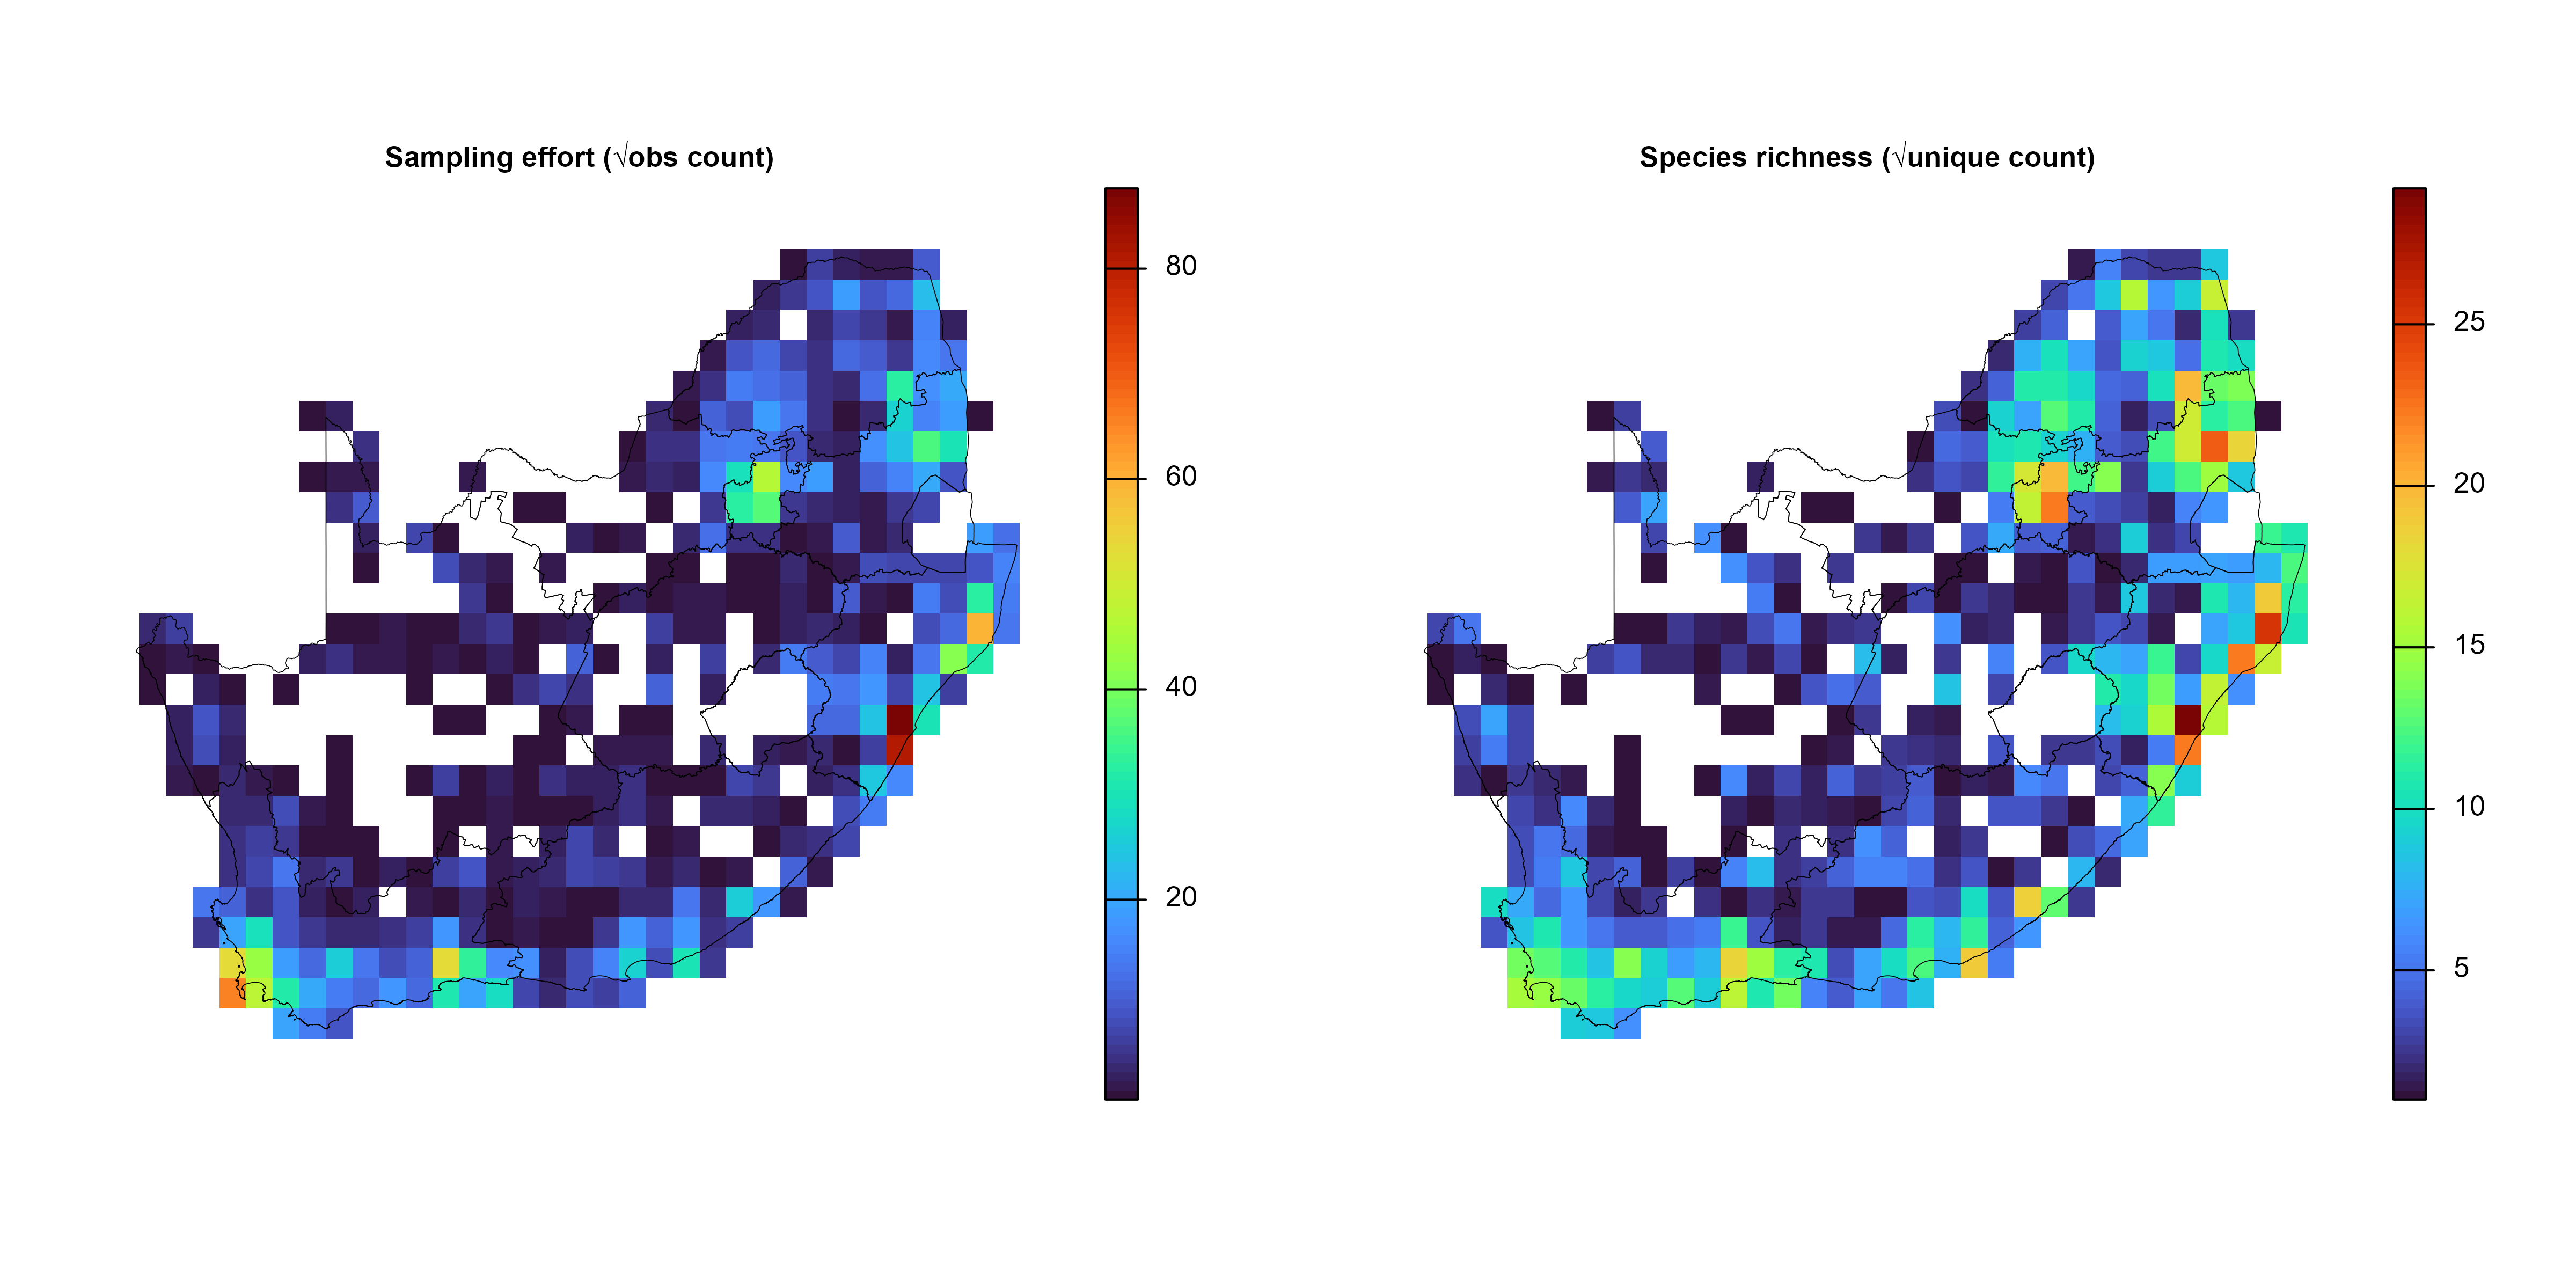
\includegraphics[width=1\linewidth]{man/figures/README-grid-1}

\begin{Shaded}
\begin{Highlighting}[]

\FunctionTok{par}\NormalTok{(old\_par)  }\CommentTok{\# reset plotting parameters}
\end{Highlighting}
\end{Shaded}

\hypertarget{retrieve-crop-resample-and-link-environmental-rasters-to-sampling-sites}{%
\subsubsection{4.5. Retrieve, crop, resample, and link environmental
rasters to sampling
sites}\label{retrieve-crop-resample-and-link-environmental-rasters-to-sampling-sites}}

Environmental predictors are appended using
\href{https://macsands.github.io/dissmapr/reference/get_enviro_data.html}{\texttt{get\_enviro\_data()}},
which buffers the grid, downloads raster data (e.g.~WorldClim
bioclimatic variables), resamples it, and links values to grid-cell
centroids. This produces both a site-by-environment data frame
(\texttt{env\_df}) and a SpatRaster object (\texttt{env\_r}), aligning
biological and environmental data.

\begin{Shaded}
\begin{Highlighting}[]
\CommentTok{\# Retrieve 19 bioclim layers (≈10{-}km, WorldClim v2.1) for all grid centroids}
\NormalTok{data\_path }\OtherTok{=} \StringTok{"inst/extdata"}               \CommentTok{\# cache folder for rasters}
\NormalTok{enviro\_list }\OtherTok{=} \FunctionTok{get\_enviro\_data}\NormalTok{(}
  \AttributeTok{data       =}\NormalTok{ grid\_spp,                  }\CommentTok{\# centroids + obs\_sum + spp\_rich}
  \AttributeTok{buffer\_km  =} \DecValTok{10}\NormalTok{,                        }\CommentTok{\# pad the AOI slightly}
  \AttributeTok{source     =} \StringTok{"geodata"}\NormalTok{,                 }\CommentTok{\# WorldClim/SoilGrids interface}
  \AttributeTok{var        =} \StringTok{"bio"}\NormalTok{,                     }\CommentTok{\# bioclim variable set}
  \AttributeTok{res        =} \DecValTok{5}\NormalTok{,                         }\CommentTok{\# 5{-}arc{-}min ≈ 10 km}
  \AttributeTok{grid\_r     =}\NormalTok{ grid\_r,                      }\CommentTok{\# To set resampling resolution, if necessary}
  \AttributeTok{path       =}\NormalTok{ data\_path,}
  \AttributeTok{sp\_cols    =} \DecValTok{7}\SpecialCharTok{:}\FunctionTok{ncol}\NormalTok{(grid\_spp),          }\CommentTok{\# ignore species columns}
  \AttributeTok{ext\_cols   =} \FunctionTok{c}\NormalTok{(}\StringTok{"obs\_sum"}\NormalTok{, }\StringTok{"spp\_rich"}\NormalTok{)   }\CommentTok{\# carry effort \& richness through}
\NormalTok{)}

\CommentTok{\# Quick checks }
\FunctionTok{str}\NormalTok{(enviro\_list, }\AttributeTok{max.level =} \DecValTok{1}\NormalTok{)}
\CommentTok{\#\textgreater{} List of 3}
\CommentTok{\#\textgreater{}  $ env\_rast:S4 class \textquotesingle{}SpatRaster\textquotesingle{} [package "terra"]}
\CommentTok{\#\textgreater{}  $ sites\_sf: sf [415 x 2] (S3: sf/tbl\_df/tbl/data.frame)}
\CommentTok{\#\textgreater{}   ..{-} attr(*, "sf\_column")= chr "geometry"}
\CommentTok{\#\textgreater{}   ..{-} attr(*, "agr")= Factor w/ 3 levels "constant","aggregate",..: NA}
\CommentTok{\#\textgreater{}   .. ..{-} attr(*, "names")= chr "grid\_id"}
\CommentTok{\#\textgreater{}  $ env\_df  : tibble [415 x 24] (S3: tbl\_df/tbl/data.frame)}

\CommentTok{\# (Optional) Assign concise layer names for readability}
\CommentTok{\# Find names here https://www.worldclim.org/data/bioclim.html}
\NormalTok{names\_env }\OtherTok{=} \FunctionTok{c}\NormalTok{(}\StringTok{"temp\_mean"}\NormalTok{,}\StringTok{"mdr"}\NormalTok{,}\StringTok{"iso"}\NormalTok{,}\StringTok{"temp\_sea"}\NormalTok{,}\StringTok{"temp\_max"}\NormalTok{,}\StringTok{"temp\_min"}\NormalTok{,}
              \StringTok{"temp\_range"}\NormalTok{,}\StringTok{"temp\_wetQ"}\NormalTok{,}\StringTok{"temp\_dryQ"}\NormalTok{,}\StringTok{"temp\_warmQ"}\NormalTok{,}
              \StringTok{"temp\_coldQ"}\NormalTok{,}\StringTok{"rain\_mean"}\NormalTok{,}\StringTok{"rain\_wet"}\NormalTok{,}\StringTok{"rain\_dry"}\NormalTok{,}
              \StringTok{"rain\_sea"}\NormalTok{,}\StringTok{"rain\_wetQ"}\NormalTok{,}\StringTok{"rain\_dryQ"}\NormalTok{,}\StringTok{"rain\_warmQ"}\NormalTok{,}\StringTok{"rain\_coldQ"}\NormalTok{)}
\FunctionTok{names}\NormalTok{(enviro\_list}\SpecialCharTok{$}\NormalTok{env\_rast) }\OtherTok{=}\NormalTok{ names\_env}

\CommentTok{\# (Optional) Promote frequently{-}used objects}
\NormalTok{env\_r }\OtherTok{=}\NormalTok{ enviro\_list}\SpecialCharTok{$}\NormalTok{env\_rast    }\CommentTok{\# cropped climate stack}
\NormalTok{env\_df }\OtherTok{=}\NormalTok{ enviro\_list}\SpecialCharTok{$}\NormalTok{env\_df      }\CommentTok{\# site × environment data{-}frame}

\CommentTok{\# Quick checks }
\NormalTok{env\_r; }\FunctionTok{dim}\NormalTok{(env\_df); }\FunctionTok{head}\NormalTok{(env\_df)}
\CommentTok{\#\textgreater{} class       : SpatRaster }
\CommentTok{\#\textgreater{} size        : 30, 37, 19  (nrow, ncol, nlyr)}
\CommentTok{\#\textgreater{} resolution  : 0.5, 0.5  (x, y)}
\CommentTok{\#\textgreater{} extent      : 15.5, 34, {-}36, {-}21  (xmin, xmax, ymin, ymax)}
\CommentTok{\#\textgreater{} coord. ref. : lon/lat WGS 84 (EPSG:4326) }
\CommentTok{\#\textgreater{} source(s)   : memory}
\CommentTok{\#\textgreater{} names       : temp\_mean,       mdr,      iso, temp\_sea, temp\_max,  temp\_min, ... }
\CommentTok{\#\textgreater{} min values  :  9.779773,  8.977007, 47.10606, 228.9986, 19.92147, {-}4.110302, ... }
\CommentTok{\#\textgreater{} max values  : 24.406433, 18.352308, 64.92966, 653.4167, 36.19497, 12.005042, ...}
\CommentTok{\#\textgreater{} [1] 415  24}
\CommentTok{\#\textgreater{} \# A tibble: 6 x 24}
\CommentTok{\#\textgreater{}   grid\_id centroid\_lon centroid\_lat bio01 bio02 bio03 bio04 bio05 bio06 bio07}
\CommentTok{\#\textgreater{}   \textless{}chr\textgreater{}          \textless{}dbl\textgreater{}        \textless{}dbl\textgreater{} \textless{}dbl\textgreater{} \textless{}dbl\textgreater{} \textless{}dbl\textgreater{} \textless{}dbl\textgreater{} \textless{}dbl\textgreater{} \textless{}dbl\textgreater{} \textless{}dbl\textgreater{}}
\CommentTok{\#\textgreater{} 1 1026            28.8        {-}22.3  21.9  14.5  55.8  425.  32.5  6.44  26.1}
\CommentTok{\#\textgreater{} 2 1027            29.2        {-}22.3  21.8  14.5  55.1  430.  32.6  6.30  26.3}
\CommentTok{\#\textgreater{} 3 1028            29.7        {-}22.3  22.0  14.2  56.3  396.  32.3  7.15  25.2}
\CommentTok{\#\textgreater{} 4 1029            30.3        {-}22.3  22.8  13.9  58.0  359.  32.7  8.79  23.9}
\CommentTok{\#\textgreater{} 5 1030            30.8        {-}22.3  23.3  13.9  60.0  332.  33.2  9.97  23.2}
\CommentTok{\#\textgreater{} 6 1031            31.3        {-}22.3  24.2  14.2  61.3  326.  34.2 10.9   23.2}
\CommentTok{\#\textgreater{} \# i 14 more variables: bio08 \textless{}dbl\textgreater{}, bio09 \textless{}dbl\textgreater{}, bio10 \textless{}dbl\textgreater{}, bio11 \textless{}dbl\textgreater{},}
\CommentTok{\#\textgreater{} \#   bio12 \textless{}dbl\textgreater{}, bio13 \textless{}dbl\textgreater{}, bio14 \textless{}dbl\textgreater{}, bio15 \textless{}dbl\textgreater{}, bio16 \textless{}dbl\textgreater{},}
\CommentTok{\#\textgreater{} \#   bio17 \textless{}dbl\textgreater{}, bio18 \textless{}dbl\textgreater{}, bio19 \textless{}dbl\textgreater{}, obs\_sum \textless{}dbl\textgreater{}, spp\_rich \textless{}dbl\textgreater{}}

\CommentTok{\# Build the final site × environment table}
\NormalTok{grid\_env }\OtherTok{=}\NormalTok{ env\_df }\SpecialCharTok{\%\textgreater{}\%}
\NormalTok{  dplyr}\SpecialCharTok{::}\FunctionTok{select}\NormalTok{(grid\_id, centroid\_lon, centroid\_lat,}
\NormalTok{                obs\_sum, spp\_rich, dplyr}\SpecialCharTok{::}\FunctionTok{everything}\NormalTok{())}

\FunctionTok{str}\NormalTok{(grid\_env, }\AttributeTok{max.level =} \DecValTok{1}\NormalTok{)}
\CommentTok{\#\textgreater{} tibble [415 x 24] (S3: tbl\_df/tbl/data.frame)}
\FunctionTok{head}\NormalTok{(grid\_env)}
\CommentTok{\#\textgreater{} \# A tibble: 6 x 24}
\CommentTok{\#\textgreater{}   grid\_id centroid\_lon centroid\_lat obs\_sum spp\_rich bio01 bio02 bio03 bio04}
\CommentTok{\#\textgreater{}   \textless{}chr\textgreater{}          \textless{}dbl\textgreater{}        \textless{}dbl\textgreater{}   \textless{}dbl\textgreater{}    \textless{}dbl\textgreater{} \textless{}dbl\textgreater{} \textless{}dbl\textgreater{} \textless{}dbl\textgreater{} \textless{}dbl\textgreater{}}
\CommentTok{\#\textgreater{} 1 1026            28.8        {-}22.3     172       17  21.9  14.5  55.8  425.}
\CommentTok{\#\textgreater{} 2 1027            29.2        {-}22.3      92        9  21.8  14.5  55.1  430.}
\CommentTok{\#\textgreater{} 3 1028            29.7        {-}22.3     131       11  22.0  14.2  56.3  396.}
\CommentTok{\#\textgreater{} 4 1029            30.3        {-}22.3     129       12  22.8  13.9  58.0  359.}
\CommentTok{\#\textgreater{} 5 1030            30.8        {-}22.3     136       13  23.3  13.9  60.0  332.}
\CommentTok{\#\textgreater{} 6 1031            31.3        {-}22.3      99       13  24.2  14.2  61.3  326.}
\CommentTok{\#\textgreater{} \# i 15 more variables: bio05 \textless{}dbl\textgreater{}, bio06 \textless{}dbl\textgreater{}, bio07 \textless{}dbl\textgreater{}, bio08 \textless{}dbl\textgreater{},}
\CommentTok{\#\textgreater{} \#   bio09 \textless{}dbl\textgreater{}, bio10 \textless{}dbl\textgreater{}, bio11 \textless{}dbl\textgreater{}, bio12 \textless{}dbl\textgreater{}, bio13 \textless{}dbl\textgreater{},}
\CommentTok{\#\textgreater{} \#   bio14 \textless{}dbl\textgreater{}, bio15 \textless{}dbl\textgreater{}, bio16 \textless{}dbl\textgreater{}, bio17 \textless{}dbl\textgreater{}, bio18 \textless{}dbl\textgreater{},}
\CommentTok{\#\textgreater{} \#   bio19 \textless{}dbl\textgreater{}}
\end{Highlighting}
\end{Shaded}

\hypertarget{remove-highly-correlated-predictors-optional}{%
\subsubsection{4.6. Remove Highly Correlated Predictors
(optional)}\label{remove-highly-correlated-predictors-optional}}

Finally,
\href{https://macsands.github.io/dissmapr/reference/rm_correlated.html}{\texttt{rm\_correlated()}}
optionally reduces multicollinearity by filtering out highly correlated
predictors based on a threshold (e.g.~r \textgreater{} 0.70), improving
model stability and interpretability. Together, these functions provide
a reproducible and scalable pipeline for preparing ecological datasets
for spatial analysis.

\begin{Shaded}
\begin{Highlighting}[]
\CommentTok{\# \# (Optional) Rename BIO}
\CommentTok{\# names(env\_df) = c("grid\_id", "centroid\_lon", "centroid\_lat", names\_env, "obs\_sum", "spp\_rich")}
\CommentTok{\#   }
\CommentTok{\# \# Run the filter and compare dimensions}
\CommentTok{\# \# Filter environmental predictors for |r| \textgreater{} 0.70}
\CommentTok{\# env\_vars\_reduced = rm\_correlated(}
\CommentTok{\#   data       = env\_df[, 4:23],  \# drop ID + coord columns}
\CommentTok{\#   cols       = NULL,                  \# infer all numeric cols}
\CommentTok{\#   threshold  = 0.70,}
\CommentTok{\#   plot       = TRUE                   \# show heat{-}map of retained vars}
\CommentTok{\# )}
\CommentTok{\# }
\CommentTok{\# \# Before vs after}
\CommentTok{\# c(original = ncol(env\_df[, c(4, 6:24)]),}
\CommentTok{\#   reduced  = ncol(env\_vars\_reduced))}
\end{Highlighting}
\end{Shaded}

\begin{center}\rule{0.5\linewidth}{0.5pt}\end{center}

\hypertarget{data-access-and-preparation-using-invasimapr}{%
\subsection{\texorpdfstring{5. Data access and preparation using
\texttt{invasimapr}}{5. Data access and preparation using invasimapr}}\label{data-access-and-preparation-using-invasimapr}}

\hypertarget{reshape-and-clean-site-by-species-observation-matrix}{%
\subsubsection{5.1. Reshape and Clean Site-by-Species Observation
Matrix}\label{reshape-and-clean-site-by-species-observation-matrix}}

This step converts the wide site-by-species abundance matrix into a
long-format data frame, suitable for downstream ecological modeling and
trait linkage. The process includes:

\begin{itemize}
\tightlist
\item
  \textbf{Dropping unnecessary metadata} (e.g., mapsheet columns)
\item
  \textbf{Pivoting to long format} so each row represents a unique
  site-species observation
\item
  \textbf{Filtering out missing species} and absent (zero count) records
\item
  \textbf{Optionally filtering} for sufficiently abundant species or
  high-confidence observations
\end{itemize}

These actions ensure your analysis is based on well-sampled taxa and
avoids downstream issues related to sparse or missing data.

\begin{Shaded}
\begin{Highlighting}[]
\CommentTok{\# Reshape site{-}by{-}species matrix to long format and clean}
\NormalTok{grid\_obs }\OtherTok{=}\NormalTok{ grid\_spp }\SpecialCharTok{\%\textgreater{}\%} 
\NormalTok{  dplyr}\SpecialCharTok{::}\FunctionTok{select}\NormalTok{(}\SpecialCharTok{{-}}\NormalTok{mapsheet) }\SpecialCharTok{\%\textgreater{}\%}                         \CommentTok{\# Drop mapsheet metadata}
  \FunctionTok{pivot\_longer}\NormalTok{(}
    \AttributeTok{cols =} \SpecialCharTok{{-}}\FunctionTok{c}\NormalTok{(grid\_id, centroid\_lon, centroid\_lat,     }\CommentTok{\# Keep core metadata columns only}
\NormalTok{              obs\_sum, spp\_rich),}
    \AttributeTok{names\_to  =} \StringTok{"species"}\NormalTok{,}
    \AttributeTok{values\_to =} \StringTok{"count"}\NormalTok{,}
    \AttributeTok{values\_drop\_na =} \ConstantTok{TRUE}\NormalTok{ ) }\SpecialCharTok{\%\textgreater{}\%}                        \CommentTok{\# Drop missing values}
  \FunctionTok{filter}\NormalTok{(count }\SpecialCharTok{\textgreater{}} \DecValTok{0}\NormalTok{) }\SpecialCharTok{\%\textgreater{}\%}                                \CommentTok{\# Remove zero{-}count (absent) records}
  \FunctionTok{relocate}\NormalTok{(grid\_id, centroid\_lon, centroid\_lat,}
\NormalTok{           obs\_sum, spp\_rich, species, count)}

\CommentTok{\# \# Only keep observations where species have \textgreater{}500 observations}
\CommentTok{\# site\_spp\_obs = site\_spp\_obs \%\textgreater{}\%}
\CommentTok{\#   \# select only the columns you care about}
\CommentTok{\#   dplyr::select(10, 13, 14, 16:17, 19, 22:23, 30:33) \%\textgreater{}\%}
\CommentTok{\#   \# drop rows where species is NA}
\CommentTok{\#   filter(!is.na(species)) \%\textgreater{}\%}
\CommentTok{\#   \# add a count column called "n\_obs"}
\CommentTok{\#   add\_count(species, name = "n\_obs") \%\textgreater{}\%}
\CommentTok{\#   \# keep only species with \textgreater{}100 observations}
\CommentTok{\#   filter(n\_obs \textgreater{} 500) \%\textgreater{}\%}
\CommentTok{\#   \# (optional) sort by descending count}
\CommentTok{\#   arrange(desc(n\_obs))}

\CommentTok{\# \# Further filter: retain only observations with count \textgreater{} 10 and non{-}missing species}
\CommentTok{\# grid\_obs = grid\_obs \%\textgreater{}\%}
\CommentTok{\#   filter(!is.na(species)) \%\textgreater{}\%}
\CommentTok{\#   filter(count \textgreater{} 10) \%\textgreater{}\%}
\CommentTok{\#   arrange(desc(count))                                 \# Optionally, sort by descending count}

\CommentTok{\# Final data check}
\CommentTok{\# Examine structure and summary statistics before further filtering}
\FunctionTok{str}\NormalTok{(grid\_obs)}
\CommentTok{\#\textgreater{} tibble [3,839 x 7] (S3: tbl\_df/tbl/data.frame)}
\CommentTok{\#\textgreater{}  $ grid\_id     : chr [1:3839] "1026" "1026" "1026" "1026" ...}
\CommentTok{\#\textgreater{}  $ centroid\_lon: num [1:3839] 28.8 28.8 28.8 28.8 28.8 ...}
\CommentTok{\#\textgreater{}  $ centroid\_lat: num [1:3839] {-}22.3 {-}22.3 {-}22.3 {-}22.3 {-}22.3 ...}
\CommentTok{\#\textgreater{}  $ obs\_sum     : num [1:3839] 172 172 172 172 172 172 172 172 172 172 ...}
\CommentTok{\#\textgreater{}  $ spp\_rich    : num [1:3839] 17 17 17 17 17 17 17 17 17 17 ...}
\CommentTok{\#\textgreater{}  $ species     : chr [1:3839] "Acraea horta" "Charaxes wakefieldi" "Danaus chrysippus orientis" "Dira clytus clytus" ...}
\CommentTok{\#\textgreater{}  $ count       : num [1:3839] 10 9 8 8 3 19 9 9 6 13 ...}
\FunctionTok{dim}\NormalTok{(grid\_obs)}
\CommentTok{\#\textgreater{} [1] 3839    7}
\FunctionTok{length}\NormalTok{(}\FunctionTok{unique}\NormalTok{(grid\_obs}\SpecialCharTok{$}\NormalTok{species))}
\CommentTok{\#\textgreater{} [1] 27}
\FunctionTok{summary}\NormalTok{(grid\_obs}\SpecialCharTok{$}\NormalTok{count)}
\CommentTok{\#\textgreater{}    Min. 1st Qu.  Median    Mean 3rd Qu.    Max. }
\CommentTok{\#\textgreater{}    1.00    6.00    9.00   10.88   14.00   87.00}
\end{Highlighting}
\end{Shaded}

\hypertarget{retrieve-and-link-trait-and-metadata-for-each-species}{%
\subsubsection{5.2. Retrieve and Link Trait and Metadata for Each
Species}\label{retrieve-and-link-trait-and-metadata-for-each-species}}

This utility provides an automated pipeline for extracting and joining
both biological trait data and rich metadata for any focal species. The
function integrates several steps:

\begin{enumerate}
\def\labelenumi{\arabic{enumi}.}
\tightlist
\item
  \textbf{Trait Table Lookup}: Retrieves species' trait data from a
  local trait table (CSV) or a
  \href{https://www.try-db.org/TryWeb/Home.php}{TRY}-style database,
  using fuzzy matching to ensure robust linkage even when there are
  minor naming inconsistencies.
\item
  \textbf{Wikipedia Metadata Scraping}: Optionally augments each species
  entry with a taxonomic summary, higher taxonomy, and representative
  images scraped directly from
  \href{https://www.wikipedia.org/}{Wikipedia}.
\item
  \textbf{Image-based Color Palette Extraction}: If enabled, downloads
  and processes public domain images to extract the most frequent
  colors, optionally removing green/white backgrounds to focus on
  diagnostic features.
\item
  \textbf{Flexible Output}: Returns a single-row tibble with the species
  name, trait data, taxonomic metadata, image URL, and color palette -
  all harmonized for downstream analyses or visualization.
\end{enumerate}

This function greatly simplifies the assembly of a unified
species-trait-metadata table, which is essential for trait-based
community ecology, macroecology, and biodiversity informatics projects.

\begin{Shaded}
\begin{Highlighting}[]
\CommentTok{\# \# Local trait data.frame version 1}
\CommentTok{\# btfly\_traits1 = read.csv("D:/Data/Traits/Butterflies/Middleton\_etal\_2020/Middleton\_etal\_2020\_traits.csv") \# adjust path}
\CommentTok{\# str(btfly\_traits1)}
\CommentTok{\# length(unique(btfly\_traits1$Species))}
\CommentTok{\# }
\CommentTok{\# \# Github trait data.frame}
\CommentTok{\# git\_url = "https://raw.githubusercontent.com/RiesLabGU/LepTraits/main/consensus/consensus.csv"}
\CommentTok{\# \# Make sure inst/extdata exists then define destination}
\CommentTok{\# dir.create("inst/extdata", recursive = TRUE, showWarnings = FALSE)}
\CommentTok{\# destfile = file.path("inst", "extdata", "consensus.csv")}
\CommentTok{\# }
\CommentTok{\# \# Download the raw CSV}
\CommentTok{\# download.file(}
\CommentTok{\#   url = git\_url,}
\CommentTok{\#   destfile = destfile,}
\CommentTok{\#   mode = "wb"    \# important on Windows}
\CommentTok{\# )}
\CommentTok{\# }
\CommentTok{\# \# 4. Read it from disk}
\CommentTok{\# btfly\_traits2 = read.csv(destfile, stringsAsFactors = FALSE)}
\CommentTok{\# str(btfly\_traits2)}
\CommentTok{\# length(unique(btfly\_traits2$Species))}
\CommentTok{\# }
\CommentTok{\# \# Retrieve and join trait/metadata for all species in the observation set}
\CommentTok{\# spp\_traits = purrr::map\_dfr(}
\CommentTok{\#   unique(grid\_obs$species),}
\CommentTok{\#   \textasciitilde{}get\_trait\_data(}
\CommentTok{\#     species = .x,}
\CommentTok{\#     remove\_bg = FALSE,}
\CommentTok{\#     n\_palette = 5,}
\CommentTok{\#     preview = FALSE,}
\CommentTok{\#     save\_folder = NULL,}
\CommentTok{\#     do\_summary = TRUE,}
\CommentTok{\#     do\_taxonomy = TRUE,}
\CommentTok{\#     do\_image = TRUE,}
\CommentTok{\#     do\_palette = TRUE,}
\CommentTok{\#     use\_try = FALSE,}
\CommentTok{\#     try\_data = NULL,}
\CommentTok{\#     \# local\_trait\_df = btfly\_traits1,}
\CommentTok{\#     local\_trait\_df = btfly\_traits2,}
\CommentTok{\#     local\_species\_col = \textquotesingle{}Species\textquotesingle{},}
\CommentTok{\#     \# github\_url = git\_url,}
\CommentTok{\#     max\_dist = 1}
\CommentTok{\#   )}
\CommentTok{\# )}

\CommentTok{\# Local trait data.frame version 2}
\NormalTok{btfly\_traits3 }\OtherTok{=} \FunctionTok{read.csv}\NormalTok{(}\StringTok{"D:/Methods/R/myR\_Packages/myCompletePks/invasimapr/inst/extdata/species\_traits.csv"}\NormalTok{) }\CommentTok{\# adjust path}
\FunctionTok{str}\NormalTok{(btfly\_traits3)}
\CommentTok{\#\textgreater{} \textquotesingle{}data.frame\textquotesingle{}:    27 obs. of  21 variables:}
\CommentTok{\#\textgreater{}  $ species     : chr  "Acraea horta" "Amata cerbera" "Bicyclus safitza safitza" "Cacyreus lingeus" ...}
\CommentTok{\#\textgreater{}  $ trait\_cont1 : num  0.83 0.874 {-}0.428 0.661 0.283 ...}
\CommentTok{\#\textgreater{}  $ trait\_cont2 : num  0.811 {-}0.106 0.672 0.475 0.622 ...}
\CommentTok{\#\textgreater{}  $ trait\_cont3 : num  {-}0.922 0.498 0.355 {-}0.657 {-}0.478 ...}
\CommentTok{\#\textgreater{}  $ trait\_cont4 : num  {-}0.684 {-}0.282 0.291 0.552 0.127 ...}
\CommentTok{\#\textgreater{}  $ trait\_cont5 : num  0.0715 {-}0.9955 0.2179 0.6736 0.503 ...}
\CommentTok{\#\textgreater{}  $ trait\_cont6 : num  0.16 0.643 {-}0.773 0.529 0.247 ...}
\CommentTok{\#\textgreater{}  $ trait\_cont7 : num  0.2035 {-}0.606 0.0705 {-}0.6409 {-}0.0962 ...}
\CommentTok{\#\textgreater{}  $ trait\_cont8 : num  {-}0.425 {-}0.611 0.568 {-}0.742 {-}0.742 ...}
\CommentTok{\#\textgreater{}  $ trait\_cont9 : num  0.1493 {-}0.2933 0.0949 0.7854 {-}0.02 ...}
\CommentTok{\#\textgreater{}  $ trait\_cont10: num  {-}0.5772 0.0992 {-}0.036 {-}0.6811 {-}0.7008 ...}
\CommentTok{\#\textgreater{}  $ trait\_cat11 : chr  "wetland" "forest" "wetland" "wetland" ...}
\CommentTok{\#\textgreater{}  $ trait\_cat12 : chr  "diurnal" "nocturnal" "diurnal" "nocturnal" ...}
\CommentTok{\#\textgreater{}  $ trait\_cat13 : chr  "bivoltine" "multivoltine" "univoltine" "multivoltine" ...}
\CommentTok{\#\textgreater{}  $ trait\_cat14 : chr  "detritivore" "detritivore" "generalist" "nectarivore" ...}
\CommentTok{\#\textgreater{}  $ trait\_cat15 : chr  "migratory" "resident" "resident" "migratory" ...}
\CommentTok{\#\textgreater{}  $ trait\_ord16 : int  4 1 4 3 4 1 1 4 1 1 ...}
\CommentTok{\#\textgreater{}  $ trait\_ord17 : int  1 4 4 3 2 4 3 5 4 3 ...}
\CommentTok{\#\textgreater{}  $ trait\_bin18 : int  1 1 1 0 1 1 1 1 0 0 ...}
\CommentTok{\#\textgreater{}  $ trait\_bin19 : int  1 0 1 0 0 1 1 1 0 1 ...}
\CommentTok{\#\textgreater{}  $ trait\_ord20 : chr  "medium" "large" "medium" "medium" ...}
\CommentTok{\# length(unique(btfly\_traits3$species))}

\CommentTok{\# Retrieve and join trait/metadata for all species in the observation set}
\NormalTok{spp\_traits }\OtherTok{=}\NormalTok{ purrr}\SpecialCharTok{::}\FunctionTok{map\_dfr}\NormalTok{(}
  \FunctionTok{unique}\NormalTok{(grid\_obs}\SpecialCharTok{$}\NormalTok{species),}
  \SpecialCharTok{\textasciitilde{}}\FunctionTok{get\_trait\_data}\NormalTok{(}
    \AttributeTok{species =}\NormalTok{ .x,}
    \AttributeTok{n\_palette =} \DecValTok{5}\NormalTok{,}
    \AttributeTok{preview =} \ConstantTok{FALSE}\NormalTok{,}
    \AttributeTok{do\_summary =} \ConstantTok{TRUE}\NormalTok{,}
    \AttributeTok{do\_taxonomy =} \ConstantTok{TRUE}\NormalTok{,}
    \AttributeTok{do\_image =} \ConstantTok{TRUE}\NormalTok{,}
    \AttributeTok{do\_palette =} \ConstantTok{TRUE}\NormalTok{,}
    \AttributeTok{local\_trait\_df =}\NormalTok{ btfly\_traits3,}
    \AttributeTok{local\_species\_col =} \StringTok{\textquotesingle{}species\textquotesingle{}}\NormalTok{,}
    \AttributeTok{max\_dist =} \DecValTok{1}
\NormalTok{  )}
\NormalTok{)}
\CommentTok{\# The final output combines trait data, taxonomic info, Wikipedia summary, images, and color palette for each species.}
\CommentTok{\# This integrated dataset supports multi{-}faceted biodiversity, trait, and visualization analyses.}

\FunctionTok{str}\NormalTok{(spp\_traits)}
\CommentTok{\#\textgreater{} tibble [27 x 29] (S3: tbl\_df/tbl/data.frame)}
\CommentTok{\#\textgreater{}  $ species     : chr [1:27] "Acraea horta" "Charaxes wakefieldi" "Danaus chrysippus orientis" "Dira clytus clytus" ...}
\CommentTok{\#\textgreater{}  $ summary     : chr [1:27] "Acraea horta or the garden acraea is a butterfly of the family Nymphalidae. It is found in South Africa and Zimbabwe." "Euxanthe wakefieldi, the forest queen, is a butterfly of the family Nymphalidae. It is found in South Africa, f"| \_\_truncated\_\_ NA "Dira clytus, the Cape autumn widow, is a butterfly of the family Nymphalidae. It is found in South Africa." ...}
\CommentTok{\#\textgreater{}  $ Kingdom     : Named chr [1:27] "Animalia" "Animalia" NA "Animalia" ...}
\CommentTok{\#\textgreater{}   ..{-} attr(*, "names")= chr [1:27] "Kingdom" "Kingdom" "Kingdom" "Kingdom" ...}
\CommentTok{\#\textgreater{}  $ Phylum      : Named chr [1:27] "Arthropoda" "Arthropoda" NA "Arthropoda" ...}
\CommentTok{\#\textgreater{}   ..{-} attr(*, "names")= chr [1:27] "Phylum" "Phylum" "Phylum" "Phylum" ...}
\CommentTok{\#\textgreater{}  $ Class       : Named chr [1:27] "Insecta" "Insecta" NA "Insecta" ...}
\CommentTok{\#\textgreater{}   ..{-} attr(*, "names")= chr [1:27] "Class" "Class" "Class" "Class" ...}
\CommentTok{\#\textgreater{}  $ Order       : Named chr [1:27] "Lepidoptera" "Lepidoptera" NA "Lepidoptera" ...}
\CommentTok{\#\textgreater{}   ..{-} attr(*, "names")= chr [1:27] "Order" "Order" "Order" "Order" ...}
\CommentTok{\#\textgreater{}  $ Family      : Named chr [1:27] "Nymphalidae" "Nymphalidae" NA "Nymphalidae" ...}
\CommentTok{\#\textgreater{}   ..{-} attr(*, "names")= chr [1:27] "Family" "Family" "Family" "Family" ...}
\CommentTok{\#\textgreater{}  $ img\_url     : chr [1:27] "https://upload.wikimedia.org/wikipedia/commons/thumb/f/fc/Garden\_acraea\_\%28Acraea\_horta\%29.jpg/250px{-}Garden\_acr"| \_\_truncated\_\_ "https://upload.wikimedia.org/wikipedia/commons/thumb/0/0f/GroseSmithKirby1892RhopExotNEPlate1\%2C\_1\%2C\_\%E2\%99\%80"| \_\_truncated\_\_ NA "https://upload.wikimedia.org/wikipedia/commons/thumb/c/ce/SeitzFaunaAfricanaXIIITaf28\%2C\_Dira\_clytus.jpg/250px{-}"| \_\_truncated\_\_ ...}
\CommentTok{\#\textgreater{}  $ palette     : chr [1:27] "\#6F782D, \#BDC57C, \#404A14, \#DE8345, \#9AA552" "\#FDFBF9, \#D1CBBE, \#644D35, \#37200C, \#988976" NA "\#4F1D09, \#885B39, \#6B3110, \#C5B091, \#FEFDFC" ...}
\CommentTok{\#\textgreater{}  $ trait\_cont1 : num [1:27] 0.8296 0.2835 0.0382 0.4732 {-}0.7307 ...}
\CommentTok{\#\textgreater{}  $ trait\_cont2 : num [1:27] 0.811 0.622 {-}0.224 0.37 {-}0.992 ...}
\CommentTok{\#\textgreater{}  $ trait\_cont3 : num [1:27] {-}0.9221 {-}0.4778 0.0288 0.3512 0.9656 ...}
\CommentTok{\#\textgreater{}  $ trait\_cont4 : num [1:27] {-}0.684 0.127 {-}0.533 {-}0.82 {-}0.829 ...}
\CommentTok{\#\textgreater{}  $ trait\_cont5 : num [1:27] 0.0715 0.503 {-}0.0945 0.0716 0.0748 ...}
\CommentTok{\#\textgreater{}  $ trait\_cont6 : num [1:27] 0.1596 0.2472 {-}0.7031 {-}0.8395 {-}0.0719 ...}
\CommentTok{\#\textgreater{}  $ trait\_cont7 : num [1:27] 0.2035 {-}0.0962 {-}0.3659 {-}0.7677 {-}0.6278 ...}
\CommentTok{\#\textgreater{}  $ trait\_cont8 : num [1:27] {-}0.4245 {-}0.7418 {-}0.8555 {-}0.8937 0.0637 ...}
\CommentTok{\#\textgreater{}  $ trait\_cont9 : num [1:27] 0.1493 {-}0.02 {-}0.6567 0.0861 0.9229 ...}
\CommentTok{\#\textgreater{}  $ trait\_cont10: num [1:27] {-}0.57722 {-}0.70084 {-}0.00145 0.88113 {-}0.33154 ...}
\CommentTok{\#\textgreater{}  $ trait\_cat11 : chr [1:27] "wetland" "forest" "grassland" "forest" ...}
\CommentTok{\#\textgreater{}  $ trait\_cat12 : chr [1:27] "diurnal" "nocturnal" "diurnal" "diurnal" ...}
\CommentTok{\#\textgreater{}  $ trait\_cat13 : chr [1:27] "bivoltine" "bivoltine" "univoltine" "bivoltine" ...}
\CommentTok{\#\textgreater{}  $ trait\_cat14 : chr [1:27] "detritivore" "generalist" "detritivore" "detritivore" ...}
\CommentTok{\#\textgreater{}  $ trait\_cat15 : chr [1:27] "migratory" "migratory" "migratory" "resident" ...}
\CommentTok{\#\textgreater{}  $ trait\_ord16 : int [1:27] 4 4 1 1 4 1 3 1 2 2 ...}
\CommentTok{\#\textgreater{}  $ trait\_ord17 : int [1:27] 1 2 4 3 5 4 1 3 5 2 ...}
\CommentTok{\#\textgreater{}  $ trait\_bin18 : int [1:27] 1 1 1 1 1 0 0 0 0 0 ...}
\CommentTok{\#\textgreater{}  $ trait\_bin19 : int [1:27] 1 0 1 1 1 0 1 0 1 1 ...}
\CommentTok{\#\textgreater{}  $ trait\_ord20 : chr [1:27] "medium" "medium" "medium" "large" ...}
\FunctionTok{head}\NormalTok{(spp\_traits)}
\CommentTok{\#\textgreater{} \# A tibble: 6 x 29}
\CommentTok{\#\textgreater{}   species  summary Kingdom Phylum Class Order Family img\_url palette trait\_cont1}
\CommentTok{\#\textgreater{}   \textless{}chr\textgreater{}    \textless{}chr\textgreater{}   \textless{}chr\textgreater{}   \textless{}chr\textgreater{}  \textless{}chr\textgreater{} \textless{}chr\textgreater{} \textless{}chr\textgreater{}  \textless{}chr\textgreater{}   \textless{}chr\textgreater{}         \textless{}dbl\textgreater{}}
\CommentTok{\#\textgreater{} 1 Acraea \textasciitilde{} Acraea\textasciitilde{} Animal\textasciitilde{} Arthr\textasciitilde{} Inse\textasciitilde{} Lepi\textasciitilde{} Nymph\textasciitilde{} https:\textasciitilde{} \#6F782\textasciitilde{}      0.830 }
\CommentTok{\#\textgreater{} 2 Charaxe\textasciitilde{} Euxant\textasciitilde{} Animal\textasciitilde{} Arthr\textasciitilde{} Inse\textasciitilde{} Lepi\textasciitilde{} Nymph\textasciitilde{} https:\textasciitilde{} \#FDFBF\textasciitilde{}      0.283 }
\CommentTok{\#\textgreater{} 3 Danaus \textasciitilde{} \textless{}NA\textgreater{}    \textless{}NA\textgreater{}    \textless{}NA\textgreater{}   \textless{}NA\textgreater{}  \textless{}NA\textgreater{}  \textless{}NA\textgreater{}   \textless{}NA\textgreater{}    \textless{}NA\textgreater{}         0.0382}
\CommentTok{\#\textgreater{} 4 Dira cl\textasciitilde{} Dira c\textasciitilde{} Animal\textasciitilde{} Arthr\textasciitilde{} Inse\textasciitilde{} Lepi\textasciitilde{} Nymph\textasciitilde{} https:\textasciitilde{} \#4F1D0\textasciitilde{}      0.473 }
\CommentTok{\#\textgreater{} 5 Eutrich\textasciitilde{} Eutric\textasciitilde{} Animal\textasciitilde{} Arthr\textasciitilde{} Inse\textasciitilde{} Lepi\textasciitilde{} Lasio\textasciitilde{} https:\textasciitilde{} \#CEAA9\textasciitilde{}     {-}0.731 }
\CommentTok{\#\textgreater{} 6 Hypolim\textasciitilde{} Hypoli\textasciitilde{} Animal\textasciitilde{} Arthr\textasciitilde{} Inse\textasciitilde{} Lepi\textasciitilde{} Nymph\textasciitilde{} https:\textasciitilde{} \#E0D5D\textasciitilde{}      0.314 }
\CommentTok{\#\textgreater{} \# i 19 more variables: trait\_cont2 \textless{}dbl\textgreater{}, trait\_cont3 \textless{}dbl\textgreater{}, trait\_cont4 \textless{}dbl\textgreater{},}
\CommentTok{\#\textgreater{} \#   trait\_cont5 \textless{}dbl\textgreater{}, trait\_cont6 \textless{}dbl\textgreater{}, trait\_cont7 \textless{}dbl\textgreater{}, trait\_cont8 \textless{}dbl\textgreater{},}
\CommentTok{\#\textgreater{} \#   trait\_cont9 \textless{}dbl\textgreater{}, trait\_cont10 \textless{}dbl\textgreater{}, trait\_cat11 \textless{}chr\textgreater{},}
\CommentTok{\#\textgreater{} \#   trait\_cat12 \textless{}chr\textgreater{}, trait\_cat13 \textless{}chr\textgreater{}, trait\_cat14 \textless{}chr\textgreater{}, trait\_cat15 \textless{}chr\textgreater{},}
\CommentTok{\#\textgreater{} \#   trait\_ord16 \textless{}int\textgreater{}, trait\_ord17 \textless{}int\textgreater{}, trait\_bin18 \textless{}int\textgreater{}, trait\_bin19 \textless{}int\textgreater{},}
\CommentTok{\#\textgreater{} \#   trait\_ord20 \textless{}chr\textgreater{}}

\CommentTok{\# Count how many non‐NA IDs}
\FunctionTok{length}\NormalTok{(}\FunctionTok{unique}\NormalTok{(btfly\_traits3}\SpecialCharTok{$}\NormalTok{species))}
\CommentTok{\#\textgreater{} [1] 27}
\FunctionTok{length}\NormalTok{(}\FunctionTok{unique}\NormalTok{(grid\_obs}\SpecialCharTok{$}\NormalTok{species))}
\CommentTok{\#\textgreater{} [1] 27}
\FunctionTok{sum}\NormalTok{(}\SpecialCharTok{!}\FunctionTok{is.na}\NormalTok{(spp\_traits}\SpecialCharTok{$}\NormalTok{species))}
\CommentTok{\#\textgreater{} [1] 27}
\end{Highlighting}
\end{Shaded}

\hypertarget{load-local-combined-site-environment-and-trait-data}{%
\subsubsection{5.3. Load local combined site, environment, and trait
data}\label{load-local-combined-site-environment-and-trait-data}}

\begin{Shaded}
\begin{Highlighting}[]
\CommentTok{\# Optional {-} Set working directory}
\FunctionTok{setwd}\NormalTok{(}\StringTok{\textquotesingle{}D:/Methods/R/myR\_Packages/myCompletePks/invasimapr/inst/extdata\textquotesingle{}}\NormalTok{)}

\CommentTok{\# Read primary data (one row per site-species combination)}
\NormalTok{site\_env\_spp }\OtherTok{=} \FunctionTok{read.csv}\NormalTok{(}\StringTok{\textquotesingle{}site\_env\_spp\_simulated.csv\textquotesingle{}}\NormalTok{)}
\FunctionTok{dim}\NormalTok{(site\_env\_spp)}
\CommentTok{\#\textgreater{} [1] 11205    36}
\FunctionTok{str}\NormalTok{(site\_env\_spp)}
\CommentTok{\#\textgreater{} \textquotesingle{}data.frame\textquotesingle{}:    11205 obs. of  36 variables:}
\CommentTok{\#\textgreater{}  $ site\_id     : int  1026 1026 1026 1026 1026 1026 1026 1026 1026 1026 ...}
\CommentTok{\#\textgreater{}  $ x           : num  28.8 28.8 28.8 28.8 28.8 ...}
\CommentTok{\#\textgreater{}  $ y           : num  {-}22.3 {-}22.3 {-}22.3 {-}22.3 {-}22.3 ...}
\CommentTok{\#\textgreater{}  $ species     : chr  "Acraea horta" "Amata cerbera" "Bicyclus safitza safitza" "Cacyreus lingeus" ...}
\CommentTok{\#\textgreater{}  $ count       : int  10 0 0 0 9 8 8 3 19 0 ...}
\CommentTok{\#\textgreater{}  $ trait\_cont1 : num  0.83 0.874 {-}0.428 0.661 0.283 ...}
\CommentTok{\#\textgreater{}  $ trait\_cont2 : num  0.811 {-}0.106 0.672 0.475 0.622 ...}
\CommentTok{\#\textgreater{}  $ trait\_cont3 : num  {-}0.922 0.498 0.355 {-}0.657 {-}0.478 ...}
\CommentTok{\#\textgreater{}  $ trait\_cont4 : num  {-}0.684 {-}0.282 0.291 0.552 0.127 ...}
\CommentTok{\#\textgreater{}  $ trait\_cont5 : num  0.0715 {-}0.9955 0.2179 0.6736 0.503 ...}
\CommentTok{\#\textgreater{}  $ trait\_cont6 : num  0.16 0.643 {-}0.773 0.529 0.247 ...}
\CommentTok{\#\textgreater{}  $ trait\_cont7 : num  0.2035 {-}0.606 0.0705 {-}0.6409 {-}0.0962 ...}
\CommentTok{\#\textgreater{}  $ trait\_cont8 : num  {-}0.425 {-}0.611 0.568 {-}0.742 {-}0.742 ...}
\CommentTok{\#\textgreater{}  $ trait\_cont9 : num  0.1493 {-}0.2933 0.0949 0.7854 {-}0.02 ...}
\CommentTok{\#\textgreater{}  $ trait\_cont10: num  {-}0.5772 0.0992 {-}0.036 {-}0.6811 {-}0.7008 ...}
\CommentTok{\#\textgreater{}  $ trait\_cat11 : chr  "wetland" "forest" "wetland" "wetland" ...}
\CommentTok{\#\textgreater{}  $ trait\_cat12 : chr  "diurnal" "nocturnal" "diurnal" "nocturnal" ...}
\CommentTok{\#\textgreater{}  $ trait\_cat13 : chr  "bivoltine" "multivoltine" "univoltine" "multivoltine" ...}
\CommentTok{\#\textgreater{}  $ trait\_cat14 : chr  "detritivore" "detritivore" "generalist" "nectarivore" ...}
\CommentTok{\#\textgreater{}  $ trait\_cat15 : chr  "migratory" "resident" "resident" "migratory" ...}
\CommentTok{\#\textgreater{}  $ trait\_ord16 : int  4 1 4 3 4 1 1 4 1 1 ...}
\CommentTok{\#\textgreater{}  $ trait\_ord17 : int  1 4 4 3 2 4 3 5 4 3 ...}
\CommentTok{\#\textgreater{}  $ trait\_bin18 : int  1 1 1 0 1 1 1 1 0 0 ...}
\CommentTok{\#\textgreater{}  $ trait\_bin19 : int  1 0 1 0 0 1 1 1 0 1 ...}
\CommentTok{\#\textgreater{}  $ trait\_ord20 : chr  "medium" "large" "medium" "medium" ...}
\CommentTok{\#\textgreater{}  $ env1        : num  2.2 2.2 2.2 2.2 2.2 ...}
\CommentTok{\#\textgreater{}  $ env2        : num  0.647 0.647 0.647 0.647 0.647 ...}
\CommentTok{\#\textgreater{}  $ env3        : num  {-}0.491 {-}0.491 {-}0.491 {-}0.491 {-}0.491 ...}
\CommentTok{\#\textgreater{}  $ env4        : num  {-}0.793 {-}0.793 {-}0.793 {-}0.793 {-}0.793 ...}
\CommentTok{\#\textgreater{}  $ env5        : num  0.822 0.822 0.822 0.822 0.822 ...}
\CommentTok{\#\textgreater{}  $ env6        : num  1.55 1.55 1.55 1.55 1.55 ...}
\CommentTok{\#\textgreater{}  $ env7        : num  0.419 0.419 0.419 0.419 0.419 ...}
\CommentTok{\#\textgreater{}  $ env8        : num  {-}1.05 {-}1.05 {-}1.05 {-}1.05 {-}1.05 ...}
\CommentTok{\#\textgreater{}  $ env9        : num  {-}0.0537 {-}0.0537 {-}0.0537 {-}0.0537 {-}0.0537 ...}
\CommentTok{\#\textgreater{}  $ env10       : num  0.933 0.933 0.933 0.933 0.933 ...}
\CommentTok{\#\textgreater{}  $ cat11\_num   : int  {-}1 1 {-}1 {-}1 1 0 1 {-}1 1 0 ...}

\CommentTok{\# \# Format \textquotesingle{}dissmapr\textquotesingle{} output to be the same}
\CommentTok{\# grid\_obs = grid\_obs \%\textgreater{}\%}
\CommentTok{\#   rename(}
\CommentTok{\#     site\_id = grid\_id,    \# Change \textquotesingle{}grid\_id\textquotesingle{} to \textquotesingle{}site\_id\textquotesingle{}}
\CommentTok{\#     x = centroid\_lon,     \# Change \textquotesingle{}centroid\_lon\textquotesingle{} to \textquotesingle{}x\textquotesingle{}}
\CommentTok{\#     y = centroid\_lat      \# Change \textquotesingle{}centroid\_lat\textquotesingle{} to \textquotesingle{}y\textquotesingle{}}
\CommentTok{\#   )}

\CommentTok{\# grid\_env = grid\_env \%\textgreater{}\%}
\CommentTok{\#   rename(}
\CommentTok{\#     site\_id = grid\_id,      \# Change \textquotesingle{}grid\_id\textquotesingle{} to \textquotesingle{}site\_id\textquotesingle{}}
\CommentTok{\#     x = centroid\_lon,     \# Change \textquotesingle{}centroid\_lon\textquotesingle{} to \textquotesingle{}x\textquotesingle{}}
\CommentTok{\#     y = centroid\_lat      \# Change \textquotesingle{}centroid\_lat\textquotesingle{} to \textquotesingle{}y\textquotesingle{}}
\CommentTok{\#   )}

\CommentTok{\# Check the results}
\FunctionTok{names}\NormalTok{(grid\_obs)}
\CommentTok{\#\textgreater{} [1] "grid\_id"      "centroid\_lon" "centroid\_lat" "obs\_sum"      "spp\_rich"    }
\CommentTok{\#\textgreater{} [6] "species"      "count"}
\CommentTok{\# names(grid\_env)}
\end{Highlighting}
\end{Shaded}

\begin{center}\rule{0.5\linewidth}{0.5pt}\end{center}

\hypertarget{model-inputs}{%
\subsection{6. Model inputs}\label{model-inputs}}

First shape your data so every row is ``one species at one site,'' with
that species' traits and that site's environment.

\hypertarget{extract-site-locations}{%
\subsubsection{\texorpdfstring{6.1. Extract
\textbf{site-locations}}{6.1. Extract site-locations}}\label{extract-site-locations}}

This section isolates the unique spatial coordinates for each sampling
site. The resulting table (\texttt{site\_xy}) will be used for spatial
mapping, distance calculations, and for merging environmental and
biodiversity metrics with precise locations.

\begin{Shaded}
\begin{Highlighting}[]
\CommentTok{\# Create site coordinate table i.e. \# Unique site coordinates}
\NormalTok{site\_xy }\OtherTok{=}\NormalTok{ site\_env\_spp }\SpecialCharTok{\%\textgreater{}\%}
\NormalTok{  dplyr}\SpecialCharTok{::}\FunctionTok{select}\NormalTok{(site\_id, x, y) }\SpecialCharTok{\%\textgreater{}\%}
  \FunctionTok{distinct}\NormalTok{() }\SpecialCharTok{\%\textgreater{}\%}
  \FunctionTok{mutate}\NormalTok{(}\AttributeTok{.site\_id\_rn =}\NormalTok{ site\_id) }\SpecialCharTok{\%\textgreater{}\%}
  \FunctionTok{column\_to\_rownames}\NormalTok{(}\AttributeTok{var =} \StringTok{".site\_id\_rn"}\NormalTok{)}
\FunctionTok{head}\NormalTok{(site\_xy)}
\CommentTok{\#\textgreater{}      site\_id     x         y}
\CommentTok{\#\textgreater{} 1026    1026 28.75 {-}22.25004}
\CommentTok{\#\textgreater{} 1027    1027 29.25 {-}22.25004}
\CommentTok{\#\textgreater{} 1028    1028 29.75 {-}22.25004}
\CommentTok{\#\textgreater{} 1029    1029 30.25 {-}22.25004}
\CommentTok{\#\textgreater{} 1030    1030 30.75 {-}22.25004}
\CommentTok{\#\textgreater{} 1031    1031 31.25 {-}22.25004}
\end{Highlighting}
\end{Shaded}

\hypertarget{extract-site-environment-variables}{%
\subsubsection{\texorpdfstring{6.2. Extract \textbf{site-environment}
variables}{6.2. Extract site-environment variables}}\label{extract-site-environment-variables}}

Here, we extract a site-by-environment matrix containing the values of
all measured environmental covariates at each sampling site. This matrix
(\texttt{site\_env}) enables analyses of environmental gradients,
spatial drivers of community composition, and covariate modeling.

\begin{Shaded}
\begin{Highlighting}[]
\CommentTok{\# Site{-}by{-}environment matrix}
\NormalTok{site\_env }\OtherTok{=}\NormalTok{ site\_env\_spp }\SpecialCharTok{\%\textgreater{}\%}
\NormalTok{  dplyr}\SpecialCharTok{::}\FunctionTok{select}\NormalTok{(site\_id, x, y,}
\NormalTok{                env1}\SpecialCharTok{:}\NormalTok{env10) }\SpecialCharTok{\%\textgreater{}\%}
  \FunctionTok{mutate}\NormalTok{(}\AttributeTok{site\_id =} \FunctionTok{as.character}\NormalTok{(site\_id)) }\SpecialCharTok{\%\textgreater{}\%}  \CommentTok{\# ensure character}
  \FunctionTok{distinct}\NormalTok{() }\SpecialCharTok{\%\textgreater{}\%}
  \FunctionTok{mutate}\NormalTok{(}\AttributeTok{.site\_id\_rn =}\NormalTok{ site\_id) }\SpecialCharTok{\%\textgreater{}\%}
  \FunctionTok{column\_to\_rownames}\NormalTok{(}\AttributeTok{var =} \StringTok{".site\_id\_rn"}\NormalTok{)}
\FunctionTok{dim}\NormalTok{(site\_env)}
\CommentTok{\#\textgreater{} [1] 415  13}
\FunctionTok{head}\NormalTok{(site\_env[}\DecValTok{1}\SpecialCharTok{:}\DecValTok{6}\NormalTok{,}\DecValTok{1}\SpecialCharTok{:}\DecValTok{6}\NormalTok{])}
\CommentTok{\#\textgreater{}      site\_id     x         y     env1      env2       env3}
\CommentTok{\#\textgreater{} 1026    1026 28.75 {-}22.25004 2.203029 0.6471631 {-}0.4910981}
\CommentTok{\#\textgreater{} 1027    1027 29.25 {-}22.25004 2.086006 1.4025519 {-}0.4471106}
\CommentTok{\#\textgreater{} 1028    1028 29.75 {-}22.25004 2.233508 0.8008731 {-}0.5405243}
\CommentTok{\#\textgreater{} 1029    1029 30.25 {-}22.25004 2.333375 1.1607272 {-}0.4405388}
\CommentTok{\#\textgreater{} 1030    1030 30.75 {-}22.25004 2.153073 1.2747649 {-}0.2945477}
\CommentTok{\#\textgreater{} 1031    1031 31.25 {-}22.25004 2.046307 1.4773531 {-}0.4125693}

\CommentTok{\# site\_env = grid\_env \%\textgreater{}\%}
\CommentTok{\#   dplyr::select(site\_id, x, y, }
\CommentTok{\#                 obs\_sum, spp\_rich, }
\CommentTok{\#                 bio01:bio19) \%\textgreater{}\%}
\CommentTok{\#   distinct() \%\textgreater{}\%}
\CommentTok{\#   mutate(.site\_id\_rn = site\_id) \%\textgreater{}\%}
\CommentTok{\#   column\_to\_rownames(var = ".site\_id\_rn")}

\FunctionTok{dim}\NormalTok{(site\_env)}
\CommentTok{\#\textgreater{} [1] 415  13}
\FunctionTok{head}\NormalTok{(site\_env[}\DecValTok{1}\SpecialCharTok{:}\DecValTok{6}\NormalTok{,}\DecValTok{1}\SpecialCharTok{:}\DecValTok{6}\NormalTok{])}
\CommentTok{\#\textgreater{}      site\_id     x         y     env1      env2       env3}
\CommentTok{\#\textgreater{} 1026    1026 28.75 {-}22.25004 2.203029 0.6471631 {-}0.4910981}
\CommentTok{\#\textgreater{} 1027    1027 29.25 {-}22.25004 2.086006 1.4025519 {-}0.4471106}
\CommentTok{\#\textgreater{} 1028    1028 29.75 {-}22.25004 2.233508 0.8008731 {-}0.5405243}
\CommentTok{\#\textgreater{} 1029    1029 30.25 {-}22.25004 2.333375 1.1607272 {-}0.4405388}
\CommentTok{\#\textgreater{} 1030    1030 30.75 {-}22.25004 2.153073 1.2747649 {-}0.2945477}
\CommentTok{\#\textgreater{} 1031    1031 31.25 {-}22.25004 2.046307 1.4773531 {-}0.4125693}
\end{Highlighting}
\end{Shaded}

\hypertarget{extract-site-species-abundances-and-presence-absence}{%
\subsubsection{\texorpdfstring{6.3. Extract \textbf{site-species}
abundances and
presence-absence}{6.3. Extract site-species abundances and presence-absence}}\label{extract-site-species-abundances-and-presence-absence}}

This section generates two site-by-species matrices: one containing
abundances (\texttt{site\_spp\_ab}), and one indicating presence-absence
(\texttt{site\_spp\_pa}). These matrices are fundamental for calculating
community diversity, richness, and for modeling occupancy and abundance
patterns.

\begin{Shaded}
\begin{Highlighting}[]
\CommentTok{\# Site{-}by{-}species abundance matrix (wide format)}
\CommentTok{\# site\_spp\_ab = grid\_obs \%\textgreater{}\%}
\NormalTok{site\_spp\_ab }\OtherTok{=}\NormalTok{ site\_env\_spp }\SpecialCharTok{\%\textgreater{}\%} \CommentTok{\# }
\NormalTok{  dplyr}\SpecialCharTok{::}\FunctionTok{select}\NormalTok{(site\_id, x, y, species, count) }\SpecialCharTok{\%\textgreater{}\%}
  \FunctionTok{pivot\_wider}\NormalTok{(}
    \AttributeTok{names\_from  =}\NormalTok{ species,}
    \AttributeTok{values\_from =}\NormalTok{ count,}
    \AttributeTok{values\_fill =} \FunctionTok{list}\NormalTok{(}\AttributeTok{count =} \DecValTok{0}\NormalTok{)}
\NormalTok{  ) }\SpecialCharTok{\%\textgreater{}\%}
  \FunctionTok{mutate}\NormalTok{(}\AttributeTok{.site\_id\_rn =}\NormalTok{ site\_id) }\SpecialCharTok{\%\textgreater{}\%}
  \FunctionTok{column\_to\_rownames}\NormalTok{(}\AttributeTok{var =} \StringTok{".site\_id\_rn"}\NormalTok{)}
\FunctionTok{dim}\NormalTok{(site\_spp\_ab)}
\CommentTok{\#\textgreater{} [1] 415  30}
\FunctionTok{head}\NormalTok{(site\_spp\_ab[}\DecValTok{1}\SpecialCharTok{:}\DecValTok{6}\NormalTok{,}\DecValTok{1}\SpecialCharTok{:}\DecValTok{6}\NormalTok{])}
\CommentTok{\#\textgreater{}      site\_id     x         y Acraea horta Amata cerbera}
\CommentTok{\#\textgreater{} 1026    1026 28.75 {-}22.25004           10             0}
\CommentTok{\#\textgreater{} 1027    1027 29.25 {-}22.25004            0             7}
\CommentTok{\#\textgreater{} 1028    1028 29.75 {-}22.25004            0             0}
\CommentTok{\#\textgreater{} 1029    1029 30.25 {-}22.25004            0            31}
\CommentTok{\#\textgreater{} 1030    1030 30.75 {-}22.25004            0            12}
\CommentTok{\#\textgreater{} 1031    1031 31.25 {-}22.25004            0             7}
\CommentTok{\#\textgreater{}      Bicyclus safitza safitza}
\CommentTok{\#\textgreater{} 1026                        0}
\CommentTok{\#\textgreater{} 1027                        0}
\CommentTok{\#\textgreater{} 1028                        0}
\CommentTok{\#\textgreater{} 1029                        0}
\CommentTok{\#\textgreater{} 1030                        3}
\CommentTok{\#\textgreater{} 1031                        0}

\CommentTok{\# Site{-}by{-}species presence/absence matrix (wide format)}
\CommentTok{\# site\_spp\_pa = grid\_obs \%\textgreater{}\%}
\NormalTok{site\_spp\_pa }\OtherTok{=}\NormalTok{ site\_env\_spp }\SpecialCharTok{\%\textgreater{}\%} 
  \FunctionTok{mutate}\NormalTok{(}\AttributeTok{pa =} \FunctionTok{as.integer}\NormalTok{(count }\SpecialCharTok{\textgreater{}} \DecValTok{0}\NormalTok{)) }\SpecialCharTok{\%\textgreater{}\%}
\NormalTok{  dplyr}\SpecialCharTok{::}\FunctionTok{select}\NormalTok{(site\_id, x, y, species, pa) }\SpecialCharTok{\%\textgreater{}\%}
  \FunctionTok{pivot\_wider}\NormalTok{(}
    \AttributeTok{names\_from  =}\NormalTok{ species,}
    \AttributeTok{values\_from =}\NormalTok{ pa,}
    \AttributeTok{values\_fill =} \FunctionTok{list}\NormalTok{(}\AttributeTok{pa =} \DecValTok{0}\NormalTok{)}
\NormalTok{  ) }\SpecialCharTok{\%\textgreater{}\%}
  \FunctionTok{mutate}\NormalTok{(}\AttributeTok{.site\_id\_rn =}\NormalTok{ site\_id) }\SpecialCharTok{\%\textgreater{}\%}
  \FunctionTok{column\_to\_rownames}\NormalTok{(}\AttributeTok{var =} \StringTok{".site\_id\_rn"}\NormalTok{)}
\FunctionTok{dim}\NormalTok{(site\_spp\_pa)}
\CommentTok{\#\textgreater{} [1] 415  30}
\FunctionTok{head}\NormalTok{(site\_spp\_pa[}\DecValTok{1}\SpecialCharTok{:}\DecValTok{6}\NormalTok{,}\DecValTok{1}\SpecialCharTok{:}\DecValTok{6}\NormalTok{])}
\CommentTok{\#\textgreater{}      site\_id     x         y Acraea horta Amata cerbera}
\CommentTok{\#\textgreater{} 1026    1026 28.75 {-}22.25004            1             0}
\CommentTok{\#\textgreater{} 1027    1027 29.25 {-}22.25004            0             1}
\CommentTok{\#\textgreater{} 1028    1028 29.75 {-}22.25004            0             0}
\CommentTok{\#\textgreater{} 1029    1029 30.25 {-}22.25004            0             1}
\CommentTok{\#\textgreater{} 1030    1030 30.75 {-}22.25004            0             1}
\CommentTok{\#\textgreater{} 1031    1031 31.25 {-}22.25004            0             1}
\CommentTok{\#\textgreater{}      Bicyclus safitza safitza}
\CommentTok{\#\textgreater{} 1026                        0}
\CommentTok{\#\textgreater{} 1027                        0}
\CommentTok{\#\textgreater{} 1028                        0}
\CommentTok{\#\textgreater{} 1029                        0}
\CommentTok{\#\textgreater{} 1030                        1}
\CommentTok{\#\textgreater{} 1031                        0}
\end{Highlighting}
\end{Shaded}

\hypertarget{extract-species-trait-values}{%
\subsubsection{\texorpdfstring{6.4. Extract \textbf{species-trait}
values}{6.4. Extract species-trait values}}\label{extract-species-trait-values}}

Here we build the species-by-trait matrix (\texttt{spp\_trait}),
including all measured continuous, categorical, and ordinal traits for
each species. This structure is central for trait-based analyses of
community assembly, functional diversity, and invasion processes.

\begin{Shaded}
\begin{Highlighting}[]
\CommentTok{\# Species{-}by{-}trait matrix (wide)}
\CommentTok{\# Extract and process continuous, categorical, and ordinal trait data}
\NormalTok{spp\_trait }\OtherTok{=}\NormalTok{ spp\_traits }\SpecialCharTok{\%\textgreater{}\%} \CommentTok{\# site\_env\_spp}
\NormalTok{  dplyr}\SpecialCharTok{::}\FunctionTok{select}\NormalTok{(species, trait\_cont1}\SpecialCharTok{:}\NormalTok{trait\_cont10, }
\NormalTok{                trait\_cat11}\SpecialCharTok{:}\NormalTok{trait\_cat15, }
\NormalTok{                trait\_ord16}\SpecialCharTok{:}\NormalTok{trait\_ord20) }\SpecialCharTok{\%\textgreater{}\%}
  \FunctionTok{distinct}\NormalTok{() }\SpecialCharTok{\%\textgreater{}\%}
  \FunctionTok{mutate}\NormalTok{(}\AttributeTok{.species\_rn =}\NormalTok{ species) }\SpecialCharTok{\%\textgreater{}\%}
  \FunctionTok{column\_to\_rownames}\NormalTok{(}\AttributeTok{var =} \StringTok{".species\_rn"}\NormalTok{) }\SpecialCharTok{\%\textgreater{}\%}
  \FunctionTok{mutate}\NormalTok{(}\FunctionTok{across}\NormalTok{(}\FunctionTok{where}\NormalTok{(is.character), as.factor))}

\FunctionTok{dim}\NormalTok{(spp\_trait)}
\CommentTok{\#\textgreater{} [1] 27 21}
\FunctionTok{head}\NormalTok{(spp\_trait[}\DecValTok{1}\SpecialCharTok{:}\DecValTok{6}\NormalTok{,}\DecValTok{1}\SpecialCharTok{:}\DecValTok{6}\NormalTok{])}
\CommentTok{\#\textgreater{}                                               species trait\_cont1 trait\_cont2}
\CommentTok{\#\textgreater{} Acraea horta                             Acraea horta   0.8296121   0.8114763}
\CommentTok{\#\textgreater{} Charaxes wakefieldi               Charaxes wakefieldi   0.2834910   0.6221103}
\CommentTok{\#\textgreater{} Danaus chrysippus orientis Danaus chrysippus orientis   0.0381919  {-}0.2237834}
\CommentTok{\#\textgreater{} Dira clytus clytus                 Dira clytus clytus   0.4731766   0.3703395}
\CommentTok{\#\textgreater{} Eutricha capensis                   Eutricha capensis  {-}0.7306668  {-}0.9921033}
\CommentTok{\#\textgreater{} Hypolimnas misippus               Hypolimnas misippus   0.3139846   0.6658322}
\CommentTok{\#\textgreater{}                            trait\_cont3 trait\_cont4 trait\_cont5}
\CommentTok{\#\textgreater{} Acraea horta               {-}0.92212702  {-}0.6841896  0.07152258}
\CommentTok{\#\textgreater{} Charaxes wakefieldi        {-}0.47782407   0.1272937  0.50304513}
\CommentTok{\#\textgreater{} Danaus chrysippus orientis  0.02882587  {-}0.5325932 {-}0.09453685}
\CommentTok{\#\textgreater{} Dira clytus clytus          0.35121455  {-}0.8200390  0.07157999}
\CommentTok{\#\textgreater{} Eutricha capensis           0.96563440  {-}0.8287759  0.07475339}
\CommentTok{\#\textgreater{} Hypolimnas misippus         0.51908854  {-}0.3895633 {-}0.99723831}
\end{Highlighting}
\end{Shaded}

\begin{center}\rule{0.5\linewidth}{0.5pt}\end{center}

\hypertarget{summarize-site-level-diversity}{%
\subsection{3. Summarize Site-Level
Diversity}\label{summarize-site-level-diversity}}

This section quantifies and visualizes site-level biodiversity, focusing
on local species richness and abundance. Calculating these metrics is
essential for mapping alpha diversity, assessing community structure,
and identifying spatial patterns of biodiversity hotspots and
low-diversity areas across the study landscape.

\begin{itemize}
\tightlist
\item
  \textbf{Species richness} (spp\_richk): the number of species present
  (non-zero counts) at site k.
\item
  \textbf{Total abundance} (obs\_sumk): the sum of all individual counts
  across species at site k (a proxy for sampling effort).
\item
  \textbf{Mean abundance per species} (obs\_meank): total abundance at
  the site divided by the number of species columns (S); effectively the
  average count per species regardless of whether it is present.
\end{itemize}

\begin{Shaded}
\begin{Highlighting}[]
\CommentTok{\# Calculate site{-}level diversity metrics from the species{-}by{-}abundance matrix:}
\NormalTok{spp\_rich\_obs }\OtherTok{=}\NormalTok{ site\_spp\_ab }\SpecialCharTok{\%\textgreater{}\%}
  \FunctionTok{mutate}\NormalTok{(}
    \AttributeTok{spp\_rich =} \FunctionTok{rowSums}\NormalTok{(dplyr}\SpecialCharTok{::}\FunctionTok{select}\NormalTok{(., }\SpecialCharTok{{-}}\NormalTok{site\_id, }\SpecialCharTok{{-}}\NormalTok{x, }\SpecialCharTok{{-}}\NormalTok{y) }\SpecialCharTok{\textgreater{}} \DecValTok{0}\NormalTok{), }\CommentTok{\# Species richness: number of species present}
    \AttributeTok{obs\_sum =} \FunctionTok{rowSums}\NormalTok{(dplyr}\SpecialCharTok{::}\FunctionTok{select}\NormalTok{(., }\SpecialCharTok{{-}}\NormalTok{site\_id, }\SpecialCharTok{{-}}\NormalTok{x, }\SpecialCharTok{{-}}\NormalTok{y)), }\CommentTok{\# Total abundance: sum of all individuals}
    \AttributeTok{obs\_mean =} \FunctionTok{rowMeans}\NormalTok{(dplyr}\SpecialCharTok{::}\FunctionTok{select}\NormalTok{(., }\SpecialCharTok{{-}}\NormalTok{site\_id, }\SpecialCharTok{{-}}\NormalTok{x, }\SpecialCharTok{{-}}\NormalTok{y)) }\CommentTok{\# Mean abundance per species}
\NormalTok{  ) }\SpecialCharTok{\%\textgreater{}\%}
  \CommentTok{\# Keep summary metrics and site coordinates}
\NormalTok{  dplyr}\SpecialCharTok{::}\FunctionTok{select}\NormalTok{(site\_id, x, y, spp\_rich, obs\_sum, obs\_mean) }\SpecialCharTok{\%\textgreater{}\%}
    \FunctionTok{mutate}\NormalTok{(}\AttributeTok{site\_id =} \FunctionTok{as.character}\NormalTok{(site\_id))  }\CommentTok{\# Ensure site\_id\textasciigrave{} is a}
\FunctionTok{head}\NormalTok{(spp\_rich\_obs)}
\CommentTok{\#\textgreater{}      site\_id     x         y spp\_rich obs\_sum obs\_mean}
\CommentTok{\#\textgreater{} 1026    1026 28.75 {-}22.25004       17     172 6.370370}
\CommentTok{\#\textgreater{} 1027    1027 29.25 {-}22.25004        9      92 3.407407}
\CommentTok{\#\textgreater{} 1028    1028 29.75 {-}22.25004       11     131 4.851852}
\CommentTok{\#\textgreater{} 1029    1029 30.25 {-}22.25004       12     129 4.777778}
\CommentTok{\#\textgreater{} 1030    1030 30.75 {-}22.25004       13     136 5.037037}
\CommentTok{\#\textgreater{} 1031    1031 31.25 {-}22.25004       13      99 3.666667}

\CommentTok{\# Define a custom color palette for richness mapping (blue = low, dark red = high)}
\NormalTok{col\_pal }\OtherTok{=} \FunctionTok{colorRampPalette}\NormalTok{(}\FunctionTok{c}\NormalTok{(}\StringTok{"blue"}\NormalTok{, }\StringTok{"green"}\NormalTok{, }\StringTok{"yellow"}\NormalTok{, }\StringTok{"orange"}\NormalTok{, }\StringTok{"red"}\NormalTok{, }\StringTok{"darkred"}\NormalTok{))}

\CommentTok{\# Visualize spatial distribution of site{-}level species richness}
\FunctionTok{ggplot}\NormalTok{(spp\_rich\_obs, }\FunctionTok{aes}\NormalTok{(}\AttributeTok{x =}\NormalTok{ x, }\AttributeTok{y =}\NormalTok{ y, }\AttributeTok{fill =} \FunctionTok{sqrt}\NormalTok{(spp\_rich))) }\SpecialCharTok{+}
  \FunctionTok{geom\_tile}\NormalTok{() }\SpecialCharTok{+}
  \CommentTok{\# Use custom color gradient, reversed so high richness is warm/dark, low is cool/blue}
  \FunctionTok{scale\_fill\_gradientn}\NormalTok{(}\AttributeTok{colors =} \FunctionTok{rev}\NormalTok{(}\FunctionTok{col\_pal}\NormalTok{(}\DecValTok{10}\NormalTok{)), }\AttributeTok{name =} \StringTok{"√(Richness)"}\NormalTok{) }\SpecialCharTok{+}
  \FunctionTok{geom\_text}\NormalTok{(}\FunctionTok{aes}\NormalTok{(}\AttributeTok{label =}\NormalTok{ spp\_rich), }\AttributeTok{color =} \StringTok{"grey80"}\NormalTok{, }\AttributeTok{size =} \DecValTok{2}\NormalTok{) }\SpecialCharTok{+} \CommentTok{\# Overlay actual richness values}
  \FunctionTok{geom\_sf}\NormalTok{(}\AttributeTok{data =}\NormalTok{ rsa, }\AttributeTok{inherit.aes =} \ConstantTok{FALSE}\NormalTok{, }\AttributeTok{fill =} \ConstantTok{NA}\NormalTok{, }\AttributeTok{color =} \StringTok{"black"}\NormalTok{, }\AttributeTok{size =} \FloatTok{0.4}\NormalTok{) }\SpecialCharTok{+}  \CommentTok{\# Plot boundary}
  \FunctionTok{labs}\NormalTok{(}
    \AttributeTok{x =} \StringTok{"Longitude"}\NormalTok{,}
    \AttributeTok{y =} \StringTok{"Latitude"}\NormalTok{,}
    \AttributeTok{title =} \StringTok{"Spatial Distribution of Species Richness"}
\NormalTok{  ) }\SpecialCharTok{+}
  \FunctionTok{theme}\NormalTok{(}\AttributeTok{panel.grid =} \FunctionTok{element\_blank}\NormalTok{())}
\end{Highlighting}
\end{Shaded}

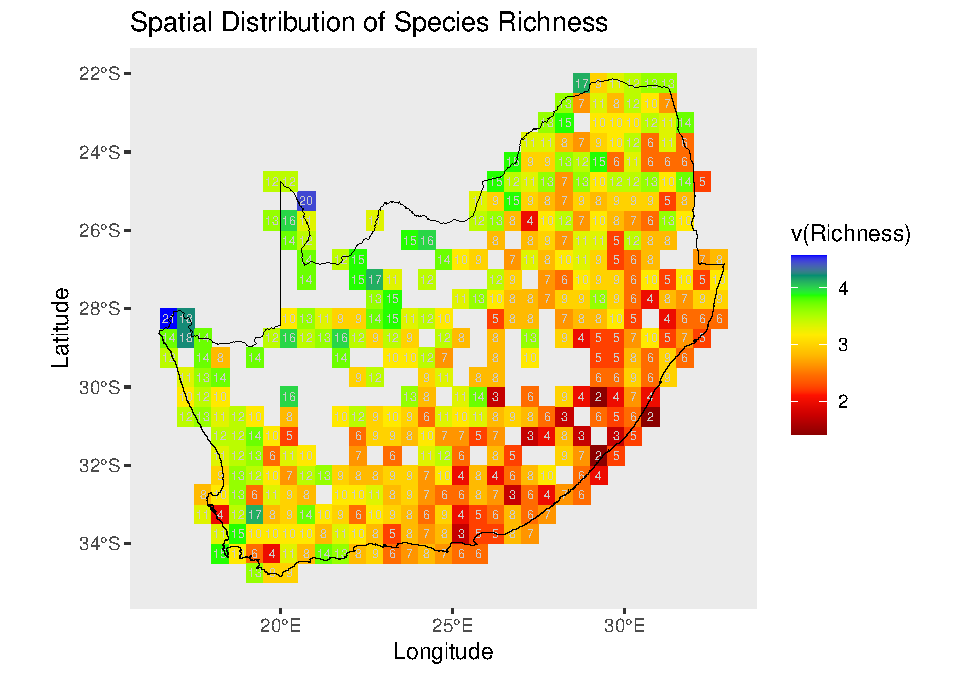
\includegraphics[width=1\linewidth]{man/figures/README-site-richness-1}

\begin{center}\rule{0.5\linewidth}{0.5pt}\end{center}

\hypertarget{similarity-functional-trait-space-and-diversity-analysis}{%
\subsection{4. Similarity, Functional Trait Space and Diversity
Analysis}\label{similarity-functional-trait-space-and-diversity-analysis}}

\hypertarget{basic-trait-similarity}{%
\subsubsection{4.1. Basic Trait
Similarity}\label{basic-trait-similarity}}

To diagnose which functional dimensions are more conserved versus
variable across the metacommunity, we compute \textbf{trait-level
similarity} for each trait across all species. This allows
identification of traits that might constrain or facilitate invasion and
coexistence (e.g., highly conserved traits might reflect strong
filtering, while highly variable traits may be axes of ecological
opportunity).

We use the \texttt{compute\_trait\_similarity()} function, which
calculates similarity as follows:

\begin{itemize}
\tightlist
\item
  \textbf{Numeric traits}: Scaled to {[}0,1{]}, pairwise Euclidean
  distances are computed, and similarity is 1 - mean(distance). If all
  values are identical or only one value is present, similarity is
  100\%.
\item
  \textbf{Categorical traits}: Similarity is the proportion of all
  possible species pairs that share the same category (level).
\end{itemize}

The output is a table of percent similarity for each trait, allowing
direct comparison of conservation vs.~lability across traits.

\begin{Shaded}
\begin{Highlighting}[]
\CommentTok{\# Compute Trait Similarity for Numeric and Categorical Variables}
\NormalTok{df\_traits }\OtherTok{=} \FunctionTok{compute\_trait\_similarity}\NormalTok{(spp\_trait[,}\SpecialCharTok{{-}}\DecValTok{1}\NormalTok{])}
\FunctionTok{head}\NormalTok{(df\_traits)}
\CommentTok{\#\textgreater{} \# A tibble: 6 x 2}
\CommentTok{\#\textgreater{}   Trait       Similarity}
\CommentTok{\#\textgreater{}   \textless{}chr\textgreater{}            \textless{}dbl\textgreater{}}
\CommentTok{\#\textgreater{} 1 trait\_cont1       61.8}
\CommentTok{\#\textgreater{} 2 trait\_cont2       63.9}
\CommentTok{\#\textgreater{} 3 trait\_cont3       65.1}
\CommentTok{\#\textgreater{} 4 trait\_cont4       64.1}
\CommentTok{\#\textgreater{} 5 trait\_cont5       69.5}
\CommentTok{\#\textgreater{} 6 trait\_cont6       62.5}

\CommentTok{\# Barplot: trait{-}level similarity (percent identity or scaled distance)}
\FunctionTok{ggplot}\NormalTok{(df\_traits, }\FunctionTok{aes}\NormalTok{(}\AttributeTok{x =} \FunctionTok{reorder}\NormalTok{(Trait, Similarity), }\AttributeTok{y =}\NormalTok{ Similarity, }\AttributeTok{fill =}\NormalTok{ Trait)) }\SpecialCharTok{+}
  \FunctionTok{geom\_col}\NormalTok{(}\AttributeTok{show.legend =} \ConstantTok{FALSE}\NormalTok{) }\SpecialCharTok{+}
  \CommentTok{\# ylim(0,100) +}
  \FunctionTok{labs}\NormalTok{(}
    \AttributeTok{title =} \StringTok{"Average Trait Similarity (\%)"}\NormalTok{,}
    \AttributeTok{y =} \StringTok{"Similarity (\%)"}\NormalTok{,}
    \AttributeTok{x =} \ConstantTok{NULL}
\NormalTok{  ) }\SpecialCharTok{+}
  \FunctionTok{theme}\NormalTok{(}\AttributeTok{axis.text.x =} \FunctionTok{element\_text}\NormalTok{(}\AttributeTok{angle =} \DecValTok{45}\NormalTok{, }\AttributeTok{hjust =} \DecValTok{1}\NormalTok{))}
\end{Highlighting}
\end{Shaded}

\begin{figure}
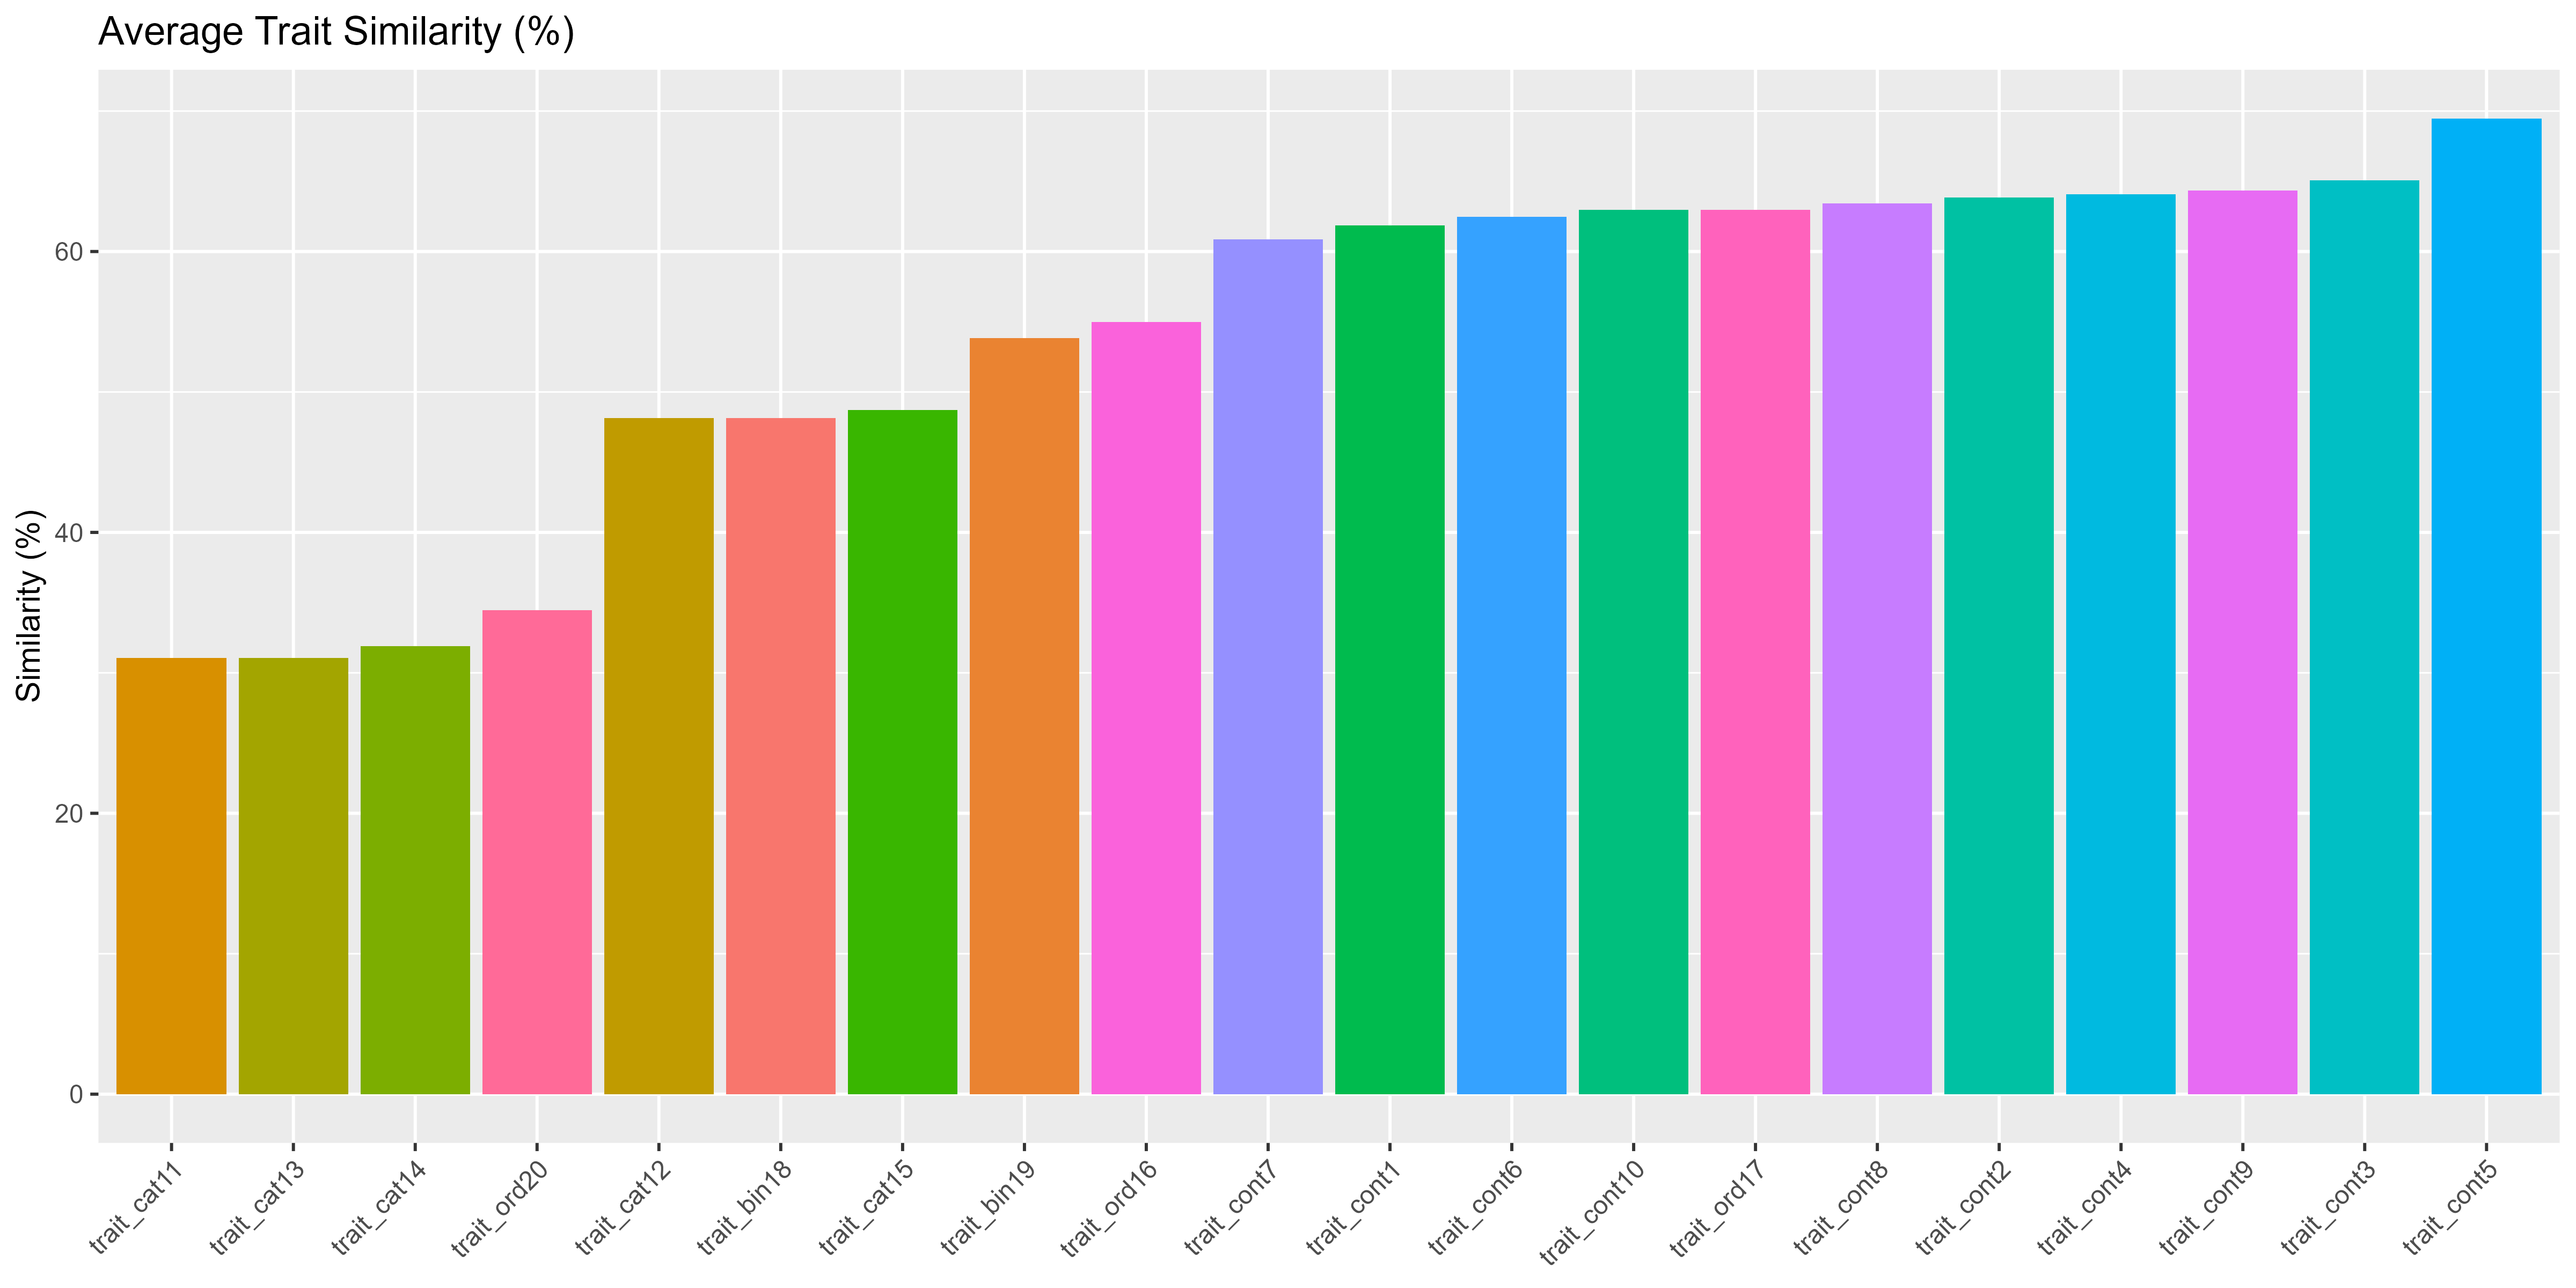
\includegraphics[width=1\linewidth]{man/figures/README-trait-sim-barplot-1} \caption{Trait-level functional similarity across species.}\label{fig:trait-sim-barplot}
\end{figure}

\hypertarget{gower-distance-and-hierarchical-clustering}{%
\subsubsection{4.2 Gower Distance and Hierarchical
Clustering}\label{gower-distance-and-hierarchical-clustering}}

Trait-based approaches require robust dissimilarity measures for mixed
data types (continuous, categorical, ordinal). Here, we compute
\textbf{pairwise Gower distances} among species, which accommodates all
variable types, and use hierarchical clustering to visualize functional
similarity structure within the community.

\begin{Shaded}
\begin{Highlighting}[]
\CommentTok{\# Compute Gower dissimilarity matrix (excluding species column)}
\NormalTok{sbt\_gower }\OtherTok{=}\NormalTok{ cluster}\SpecialCharTok{::}\FunctionTok{daisy}\NormalTok{(spp\_trait[,}\SpecialCharTok{{-}}\DecValTok{1}\NormalTok{], }\AttributeTok{metric =} \StringTok{"gower"}\NormalTok{)}
\NormalTok{trait\_dist }\OtherTok{=} \FunctionTok{as.matrix}\NormalTok{(sbt\_gower)}

\CommentTok{\# Hierarchical clustering and dendrogram visualization of functional similarity}
\CommentTok{\# Hierarchical clustering}
\NormalTok{gower\_hc }\OtherTok{=} \FunctionTok{hclust}\NormalTok{(}\FunctionTok{as.dist}\NormalTok{(sbt\_gower))}
\CommentTok{\# Dendrogram}
\FunctionTok{fviz\_dend}\NormalTok{(}
\NormalTok{  gower\_hc,}
  \AttributeTok{k =} \DecValTok{4}\NormalTok{,}
  \AttributeTok{cex =} \FloatTok{0.5}\NormalTok{,}
  \AttributeTok{k\_colors =} \FunctionTok{viridis}\NormalTok{(}\DecValTok{4}\NormalTok{, }\AttributeTok{option =} \StringTok{"D"}\NormalTok{), }\CommentTok{\# k\_colors = c("red","blue","green","purple"),}
  \AttributeTok{color\_labels\_by\_k =} \ConstantTok{TRUE}\NormalTok{,}
  \AttributeTok{rect =} \ConstantTok{TRUE}\NormalTok{,}
  \AttributeTok{rect\_border =} \StringTok{"grey40"}\NormalTok{,}
  \AttributeTok{main =} \StringTok{"Gower Cluster Dendrogram"}\NormalTok{) }\SpecialCharTok{+} 
  \FunctionTok{guides}\NormalTok{(}\AttributeTok{scale =} \StringTok{"none"}\NormalTok{)}
\end{Highlighting}
\end{Shaded}

\begin{figure}
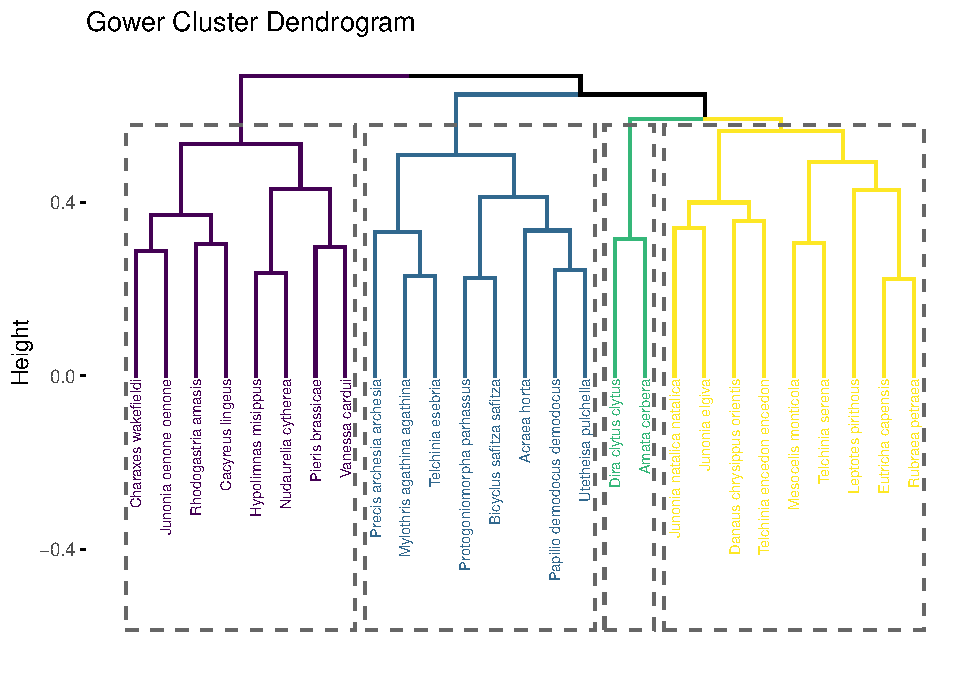
\includegraphics[width=1\linewidth]{man/figures/README-gower-dendro-1} \caption{Species clustering by functional traits (Gower distance, hierarchical clustering).}\label{fig:gower-dendro}
\end{figure}

\hypertarget{trait-space-mapping-via-principal-coordinates-analysis-pcoa}{%
\subsubsection{4.3. Trait Space Mapping via Principal Coordinates
Analysis
(PCoA)}\label{trait-space-mapping-via-principal-coordinates-analysis-pcoa}}

Principal Coordinates Analysis (PCoA) enables \textbf{ordination} of
species in a reduced, low-dimensional trait space, preserving pairwise
dissimilarities. This is used to visualize the overall structure of the
functional trait space and examine density and clustering patterns.

\begin{Shaded}
\begin{Highlighting}[]
\CommentTok{\# PCoA ordination}
\NormalTok{pcoa }\OtherTok{=} \FunctionTok{cmdscale}\NormalTok{(sbt\_gower, }\AttributeTok{eig =} \ConstantTok{TRUE}\NormalTok{)}
\NormalTok{scores\_species }\OtherTok{=} \FunctionTok{as.data.frame}\NormalTok{(pcoa}\SpecialCharTok{$}\NormalTok{points)[,}\DecValTok{1}\SpecialCharTok{:}\DecValTok{2}\NormalTok{]}
\FunctionTok{colnames}\NormalTok{(scores\_species) }\OtherTok{=} \FunctionTok{c}\NormalTok{(}\StringTok{"PCoA1"}\NormalTok{, }\StringTok{"PCoA2"}\NormalTok{)}

\CommentTok{\# Visualize trait space density using kernel density estimation}
\NormalTok{xlims }\OtherTok{=} \FunctionTok{range}\NormalTok{(scores\_species}\SpecialCharTok{$}\NormalTok{PCoA1) }\SpecialCharTok{+} \FunctionTok{c}\NormalTok{(}\SpecialCharTok{{-}}\DecValTok{1}\NormalTok{, }\DecValTok{1}\NormalTok{) }\SpecialCharTok{*} \FloatTok{0.1} \SpecialCharTok{*} \FunctionTok{diff}\NormalTok{(}\FunctionTok{range}\NormalTok{(scores\_species}\SpecialCharTok{$}\NormalTok{PCoA1))}
\NormalTok{ylims }\OtherTok{=} \FunctionTok{range}\NormalTok{(scores\_species}\SpecialCharTok{$}\NormalTok{PCoA2) }\SpecialCharTok{+} \FunctionTok{c}\NormalTok{(}\SpecialCharTok{{-}}\DecValTok{1}\NormalTok{, }\DecValTok{1}\NormalTok{) }\SpecialCharTok{*} \FloatTok{0.1} \SpecialCharTok{*} \FunctionTok{diff}\NormalTok{(}\FunctionTok{range}\NormalTok{(scores\_species}\SpecialCharTok{$}\NormalTok{PCoA2))}
\NormalTok{grid\_density }\OtherTok{=}\NormalTok{ MASS}\SpecialCharTok{::}\FunctionTok{kde2d}\NormalTok{(scores\_species}\SpecialCharTok{$}\NormalTok{PCoA1, }
\NormalTok{                           scores\_species}\SpecialCharTok{$}\NormalTok{PCoA2, }
                           \AttributeTok{n =} \DecValTok{100}\NormalTok{, }
                           \AttributeTok{lims =} \FunctionTok{c}\NormalTok{(xlims, ylims))}
\FunctionTok{filled.contour}\NormalTok{(}
\NormalTok{  grid\_density,}
  \AttributeTok{color.palette =}\NormalTok{ viridis,}
  \AttributeTok{xlim =}\NormalTok{ xlims, }\AttributeTok{ylim =}\NormalTok{ ylims,}
  \AttributeTok{plot.title =} \FunctionTok{title}\NormalTok{(}
    \AttributeTok{main =} \StringTok{"Trait Space Density Contours"}\NormalTok{,}
    \AttributeTok{xlab =} \StringTok{"PCoA1"}\NormalTok{,}
    \AttributeTok{ylab =} \StringTok{"PCoA2"}
\NormalTok{  ),}
  \AttributeTok{plot.axes =}\NormalTok{ \{}
    \FunctionTok{axis}\NormalTok{(}\DecValTok{1}\NormalTok{); }\FunctionTok{axis}\NormalTok{(}\DecValTok{2}\NormalTok{)}
    \FunctionTok{points}\NormalTok{(scores\_species, }\AttributeTok{pch =} \DecValTok{19}\NormalTok{, }\AttributeTok{cex =} \FloatTok{0.5}\NormalTok{)}
    \CommentTok{\# Draw all contours (thin)}
    \FunctionTok{contour}\NormalTok{(}
      \AttributeTok{x =}\NormalTok{ grid\_density}\SpecialCharTok{$}\NormalTok{x, }\AttributeTok{y =}\NormalTok{ grid\_density}\SpecialCharTok{$}\NormalTok{y, }\AttributeTok{z =}\NormalTok{ grid\_density}\SpecialCharTok{$}\NormalTok{z,}
      \AttributeTok{add =} \ConstantTok{TRUE}\NormalTok{, }\AttributeTok{drawlabels =} \ConstantTok{FALSE}\NormalTok{, }\AttributeTok{lwd =} \FloatTok{0.7}\NormalTok{, }\AttributeTok{col =} \StringTok{"grey60"}
\NormalTok{    )}
    \CommentTok{\# Highlight the major contour (e.g. highest density level)}
    \FunctionTok{contour}\NormalTok{(}
      \AttributeTok{x =}\NormalTok{ grid\_density}\SpecialCharTok{$}\NormalTok{x, }\AttributeTok{y =}\NormalTok{ grid\_density}\SpecialCharTok{$}\NormalTok{y, }\AttributeTok{z =}\NormalTok{ grid\_density}\SpecialCharTok{$}\NormalTok{z,}
      \AttributeTok{add =} \ConstantTok{TRUE}\NormalTok{, }\AttributeTok{drawlabels =} \ConstantTok{FALSE}\NormalTok{,}
      \AttributeTok{levels =} \FunctionTok{max}\NormalTok{(grid\_density}\SpecialCharTok{$}\NormalTok{z) }\SpecialCharTok{*} \FloatTok{0.5}\NormalTok{,  }\CommentTok{\# 50\% of max density}
      \AttributeTok{lwd =} \DecValTok{2}\NormalTok{, }\AttributeTok{col =} \StringTok{"black"}
\NormalTok{    )}
\NormalTok{  \},}
  \AttributeTok{key.title =} \FunctionTok{title}\NormalTok{(}\AttributeTok{main =} \StringTok{"Density"}\NormalTok{)}
\NormalTok{)}
\end{Highlighting}
\end{Shaded}

\begin{figure}
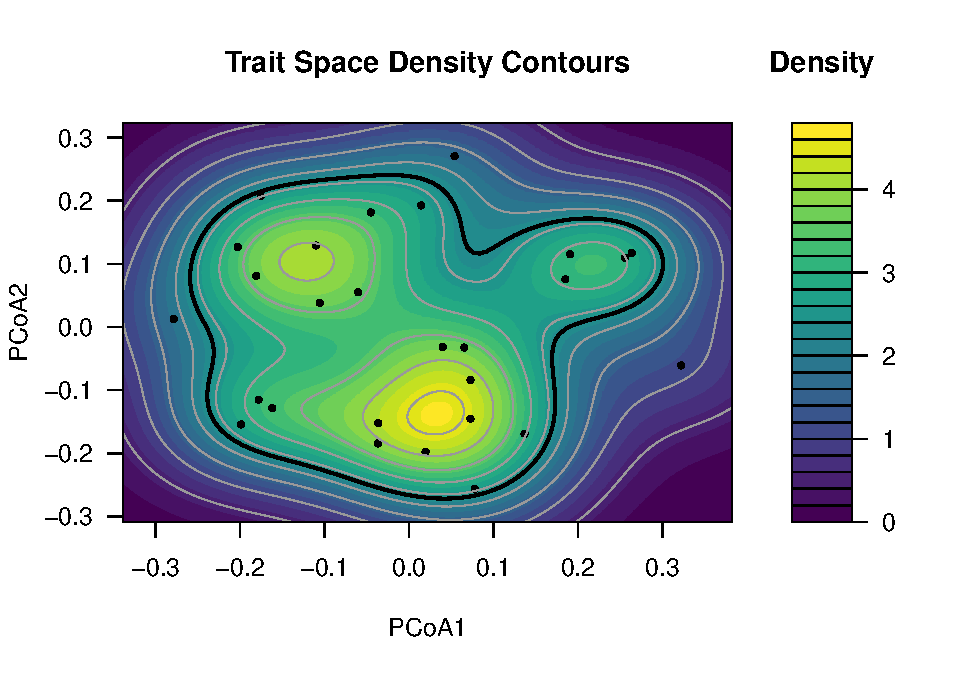
\includegraphics[width=1\linewidth]{man/figures/README-pcoa-traitspace-1} \caption{Kernel density in trait space (PCoA axes 1-2).}\label{fig:pcoa-traitspace}
\end{figure}

\hypertarget{trait-centrality}{%
\subsubsection{4.4. Trait Centrality}\label{trait-centrality}}

Trait \textbf{centrality} quantifies how close each species is to the
``core'' of the community's trait space. Peripheral species may be
ecologically distinct and potentially more likely to become invaders or
to escape biotic resistance.

\begin{Shaded}
\begin{Highlighting}[]
\CommentTok{\# Calculate the community trait centroid in reduced trait{-}space (PCoA axes)}
\NormalTok{centroid }\OtherTok{=} \FunctionTok{colMeans}\NormalTok{(scores\_species)}

\CommentTok{\# Compute each species\textquotesingle{} Euclidean distance to the centroid (trait centrality)}
\NormalTok{scores\_species}\SpecialCharTok{$}\NormalTok{centrality }\OtherTok{=} \FunctionTok{sqrt}\NormalTok{(}\FunctionTok{rowSums}\NormalTok{((scores\_species }\SpecialCharTok{{-}}\NormalTok{ centroid)}\SpecialCharTok{\^{}}\DecValTok{2}\NormalTok{))}

\CommentTok{\# Add centrality to the main trait data frame for further analysis/plotting}
\NormalTok{spp\_trt\_cent }\OtherTok{=}\NormalTok{ spp\_trait}
\NormalTok{spp\_trt\_cent}\SpecialCharTok{$}\NormalTok{centrality }\OtherTok{=}\NormalTok{ scores\_species}\SpecialCharTok{$}\NormalTok{centrality}

\CommentTok{\# Histogram of distribution of trait centrality (core vs peripheral species)}
\FunctionTok{ggplot}\NormalTok{(spp\_trt\_cent, }\FunctionTok{aes}\NormalTok{(}\AttributeTok{x =}\NormalTok{ centrality)) }\SpecialCharTok{+}
  \FunctionTok{geom\_histogram}\NormalTok{(}\AttributeTok{bins =} \DecValTok{20}\NormalTok{, }\AttributeTok{fill =} \StringTok{"steelblue"}\NormalTok{, }\AttributeTok{color =} \StringTok{"white"}\NormalTok{) }\SpecialCharTok{+}
  \FunctionTok{theme\_bw}\NormalTok{() }\SpecialCharTok{+}
  \FunctionTok{labs}\NormalTok{(}\AttributeTok{x =} \StringTok{"Distance to community{-}centroid"}\NormalTok{, }\AttributeTok{y =} \StringTok{"Number of species"}\NormalTok{,}
       \AttributeTok{title =} \StringTok{"Trait Centrality (Community Edge vs Core)"}\NormalTok{)}
\end{Highlighting}
\end{Shaded}

\begin{figure}
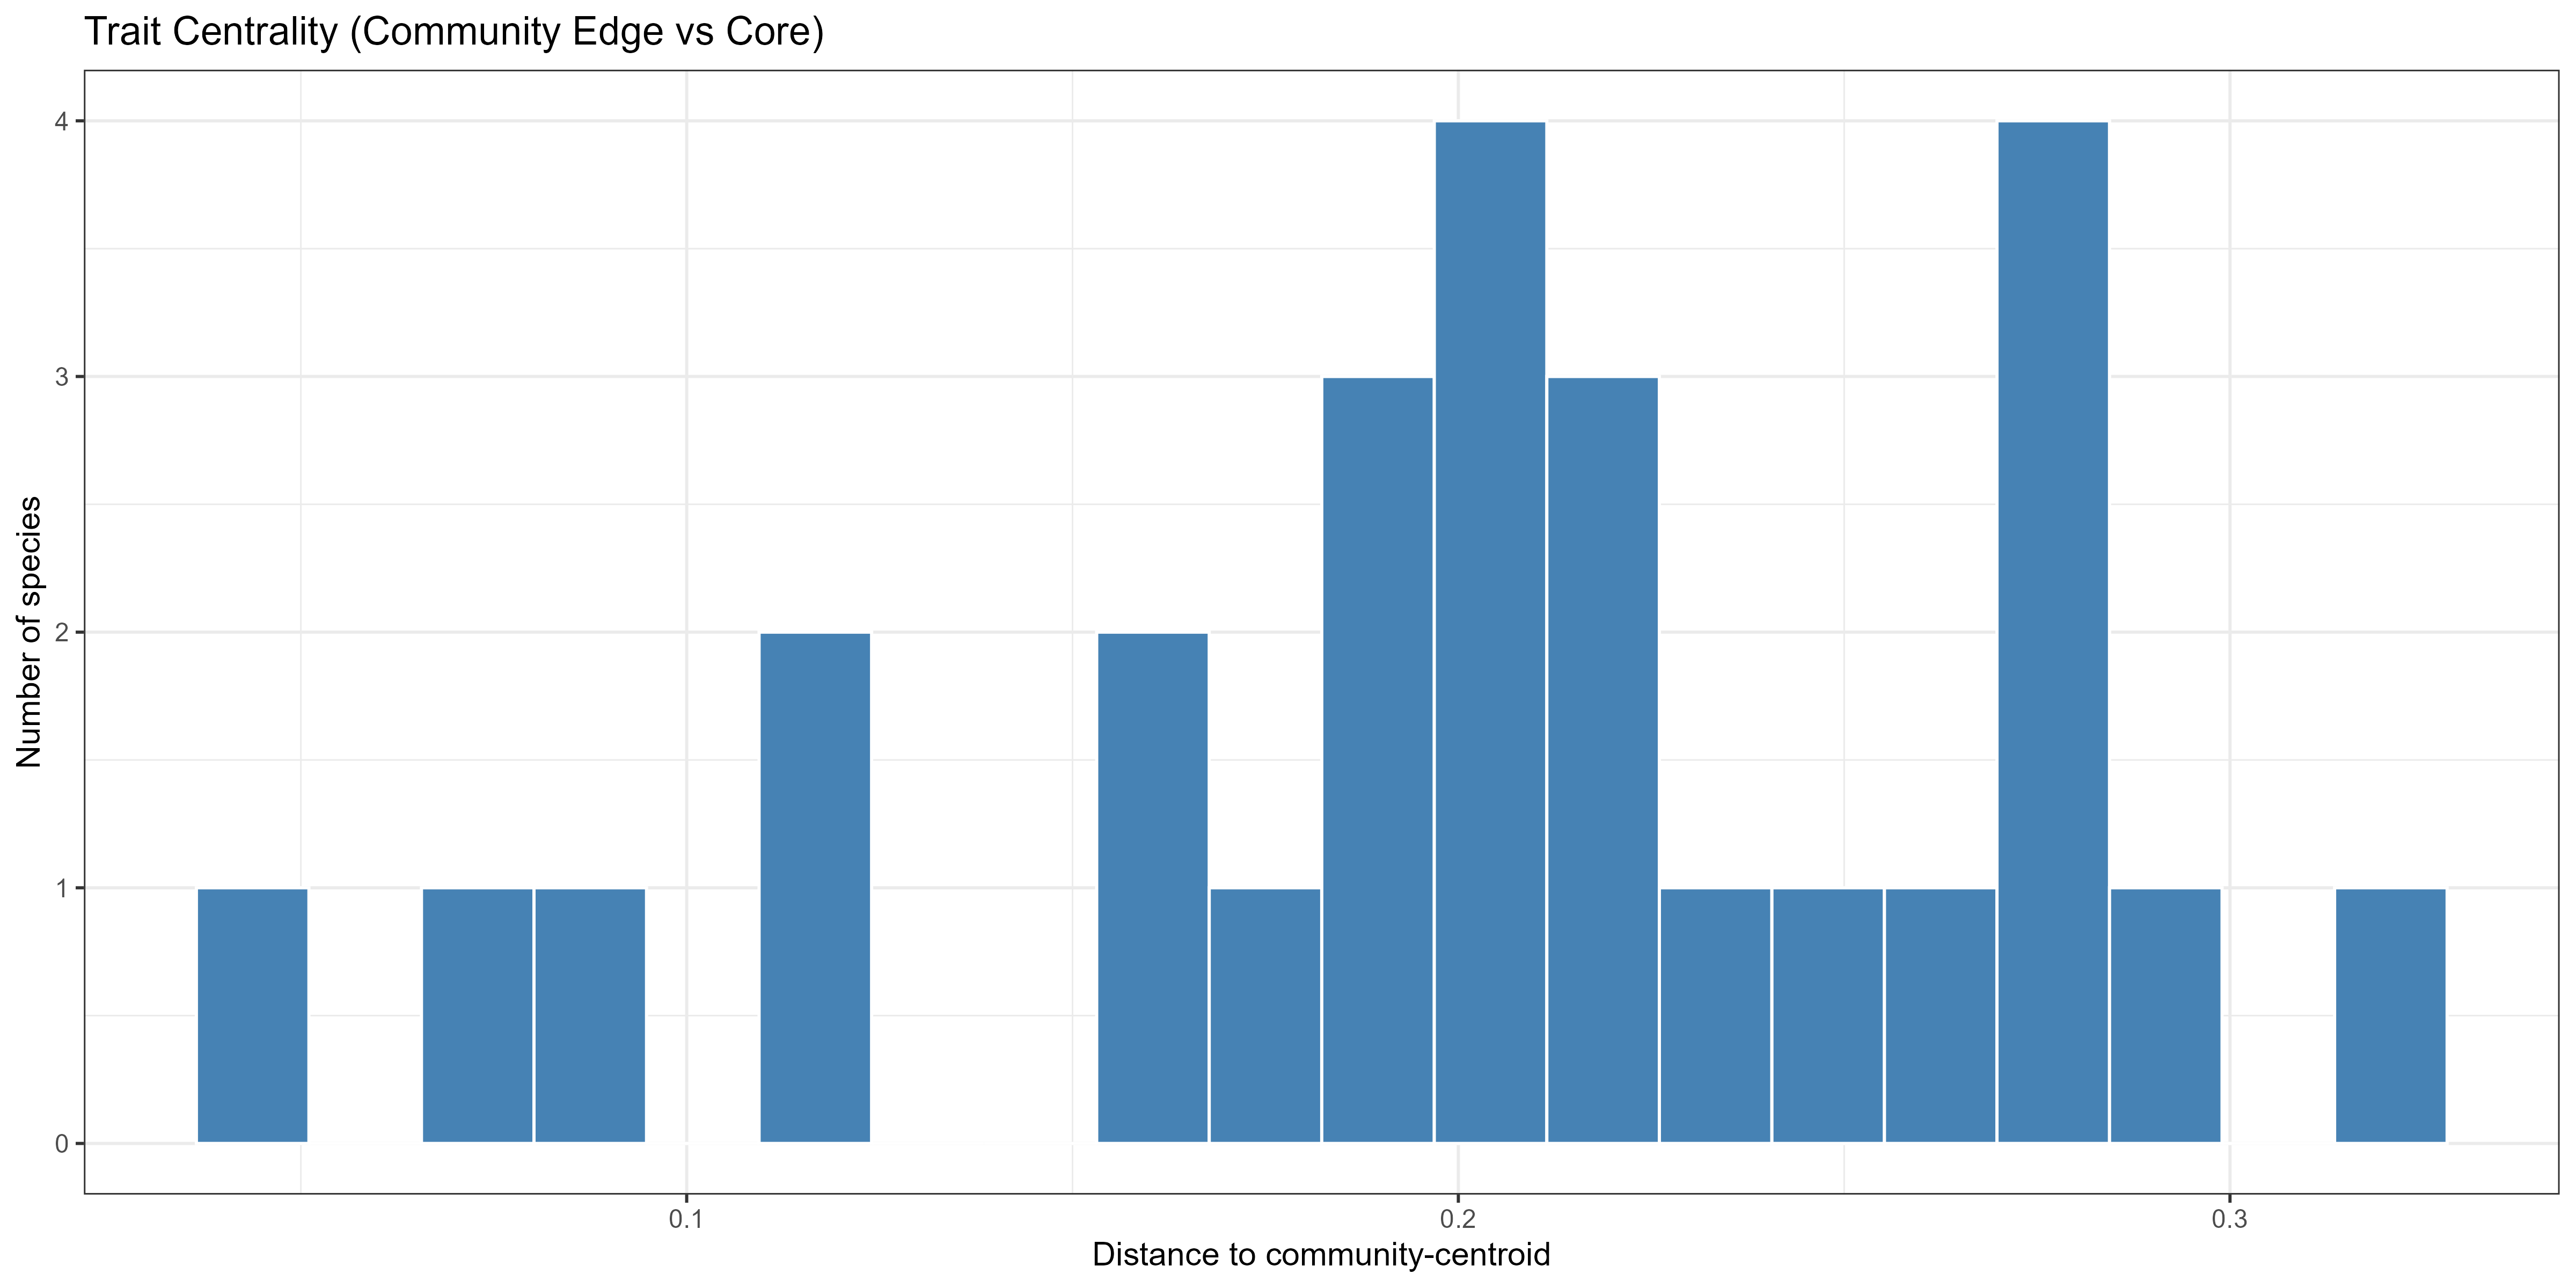
\includegraphics[width=1\linewidth]{man/figures/README-trait-centrality-1} \caption{Distribution of trait centrality (distance to centroid) among species.}\label{fig:trait-centrality}
\end{figure}

\begin{Shaded}
\begin{Highlighting}[]

\CommentTok{\# \# OPTIONAL}
\CommentTok{\# \# Scatterplot of trait{-}space (PCoA1 vs PCoA2), coloured by trait centrality}
\CommentTok{\# ggplot(scores\_species, aes(x = PCoA1, y = PCoA2, colour = centrality)) +}
\CommentTok{\#   geom\_point(size = 3) +}
\CommentTok{\#   scale\_colour\_viridis\_c(option = "magma") +}
\CommentTok{\#   labs(colour = "Centrality",}
\CommentTok{\#        title = "Species Position in Trait Space (PCoA axes 1-2)")}
\end{Highlighting}
\end{Shaded}

\begin{quote}
This histogram shows how far each species is from the \textbf{center} of
the community's trait space.

\begin{itemize}
\tightlist
\item
  The \textbf{x-axis} is \emph{distance to the centroid} (central trait
  combination of the community).
\item
  The \textbf{y-axis} is the number of species at each distance.
\end{itemize}

\textbf{Interpretation:}

\begin{itemize}
\tightlist
\item
  Most species are clustered at \textbf{intermediate distances}
  (\textasciitilde0.18--0.22), meaning their traits are moderately
  similar to the community average.
\item
  A few species are \textbf{very close} to the centroid (low distances)
  - these are ``core'' species with typical trait values.\\
\item
  Others lie \textbf{further out} (higher distances) - these are
  ``peripheral'' species with more unusual trait combinations, which
  might indicate unique ecological roles or specialisations.
\end{itemize}

\textbf{Summary}: the community is centred around a typical trait set,
but also includes a handful of species that are either very similar or
quite distinct from that average.
\end{quote}

\hypertarget{community-level-trait-dispersion}{%
\subsubsection{4.5. Community-Level Trait
Dispersion}\label{community-level-trait-dispersion}}

We calculate key functional diversity metrics at the community scale:

\begin{itemize}
\tightlist
\item
  \textbf{FDis}: functional \textbf{dispersion} (average distance to
  centroid)
\item
  \textbf{FRic}: functional richness (trait-space convex hull volume)
\item
  \textbf{RaoQ}: Rao's quadratic entropy (total abundance-weighted trait
  dissimilarity)
\end{itemize}

These summarize the functional structure and ecological breadth of the
community.

\begin{Shaded}
\begin{Highlighting}[]
\CommentTok{\# FDis: Functional dispersion (mean distance to centroid in trait space)}
\NormalTok{FDis }\OtherTok{=} \FunctionTok{mean}\NormalTok{(scores\_species}\SpecialCharTok{$}\NormalTok{centrality)}

\CommentTok{\# FRic: Functional richness (convex hull volume in PCoA space)}
\NormalTok{hull }\OtherTok{=} \FunctionTok{convhulln}\NormalTok{(scores\_species, }\AttributeTok{options =} \StringTok{"FA"}\NormalTok{)}
\NormalTok{FRic }\OtherTok{=}\NormalTok{ hull}\SpecialCharTok{$}\NormalTok{vol}

\CommentTok{\# Rao\textquotesingle{}s Q: Rao\textquotesingle{}s quadratic entropy (abundance{-}weighted pairwise trait diversity)}
\NormalTok{n }\OtherTok{=} \FunctionTok{nrow}\NormalTok{(scores\_species)}
\NormalTok{dmat }\OtherTok{=} \FunctionTok{as.matrix}\NormalTok{(}\FunctionTok{dist}\NormalTok{(scores\_species))}
\NormalTok{p }\OtherTok{=} \FunctionTok{rep}\NormalTok{(}\DecValTok{1}\SpecialCharTok{/}\NormalTok{n, n)}
\NormalTok{RaoQ }\OtherTok{=} \FloatTok{0.5} \SpecialCharTok{*} \FunctionTok{sum}\NormalTok{(}\FunctionTok{outer}\NormalTok{(p, p) }\SpecialCharTok{*}\NormalTok{ dmat)}

\CommentTok{\# Assemble all community{-}level trait dispersion metrics for comparison}
\NormalTok{dispersion\_df }\OtherTok{=} \FunctionTok{data.frame}\NormalTok{(}
  \AttributeTok{Metric =} \FunctionTok{c}\NormalTok{(}\StringTok{"FDis"}\NormalTok{, }\StringTok{"FRic"}\NormalTok{, }\StringTok{"RaoQ"}\NormalTok{),}
  \AttributeTok{Value =} \FunctionTok{c}\NormalTok{(FDis, FRic, RaoQ)}
\NormalTok{)}

\CommentTok{\# Bar plot: community{-}level trait dispersion metrics}
\FunctionTok{ggplot}\NormalTok{(dispersion\_df, }\FunctionTok{aes}\NormalTok{(}\AttributeTok{x =}\NormalTok{ Metric, }\AttributeTok{y =}\NormalTok{ Value)) }\SpecialCharTok{+}
  \FunctionTok{geom\_col}\NormalTok{(}\AttributeTok{width =} \FloatTok{0.6}\NormalTok{, }\AttributeTok{fill =} \StringTok{"firebrick"}\NormalTok{) }\SpecialCharTok{+}
  \FunctionTok{theme\_classic}\NormalTok{() }\SpecialCharTok{+}
  \FunctionTok{labs}\NormalTok{(}\AttributeTok{title =} \StringTok{"Community{-}Level Trait Dispersion"}\NormalTok{, }\AttributeTok{y =} \StringTok{"Metric value"}\NormalTok{)}
\end{Highlighting}
\end{Shaded}

\begin{figure}
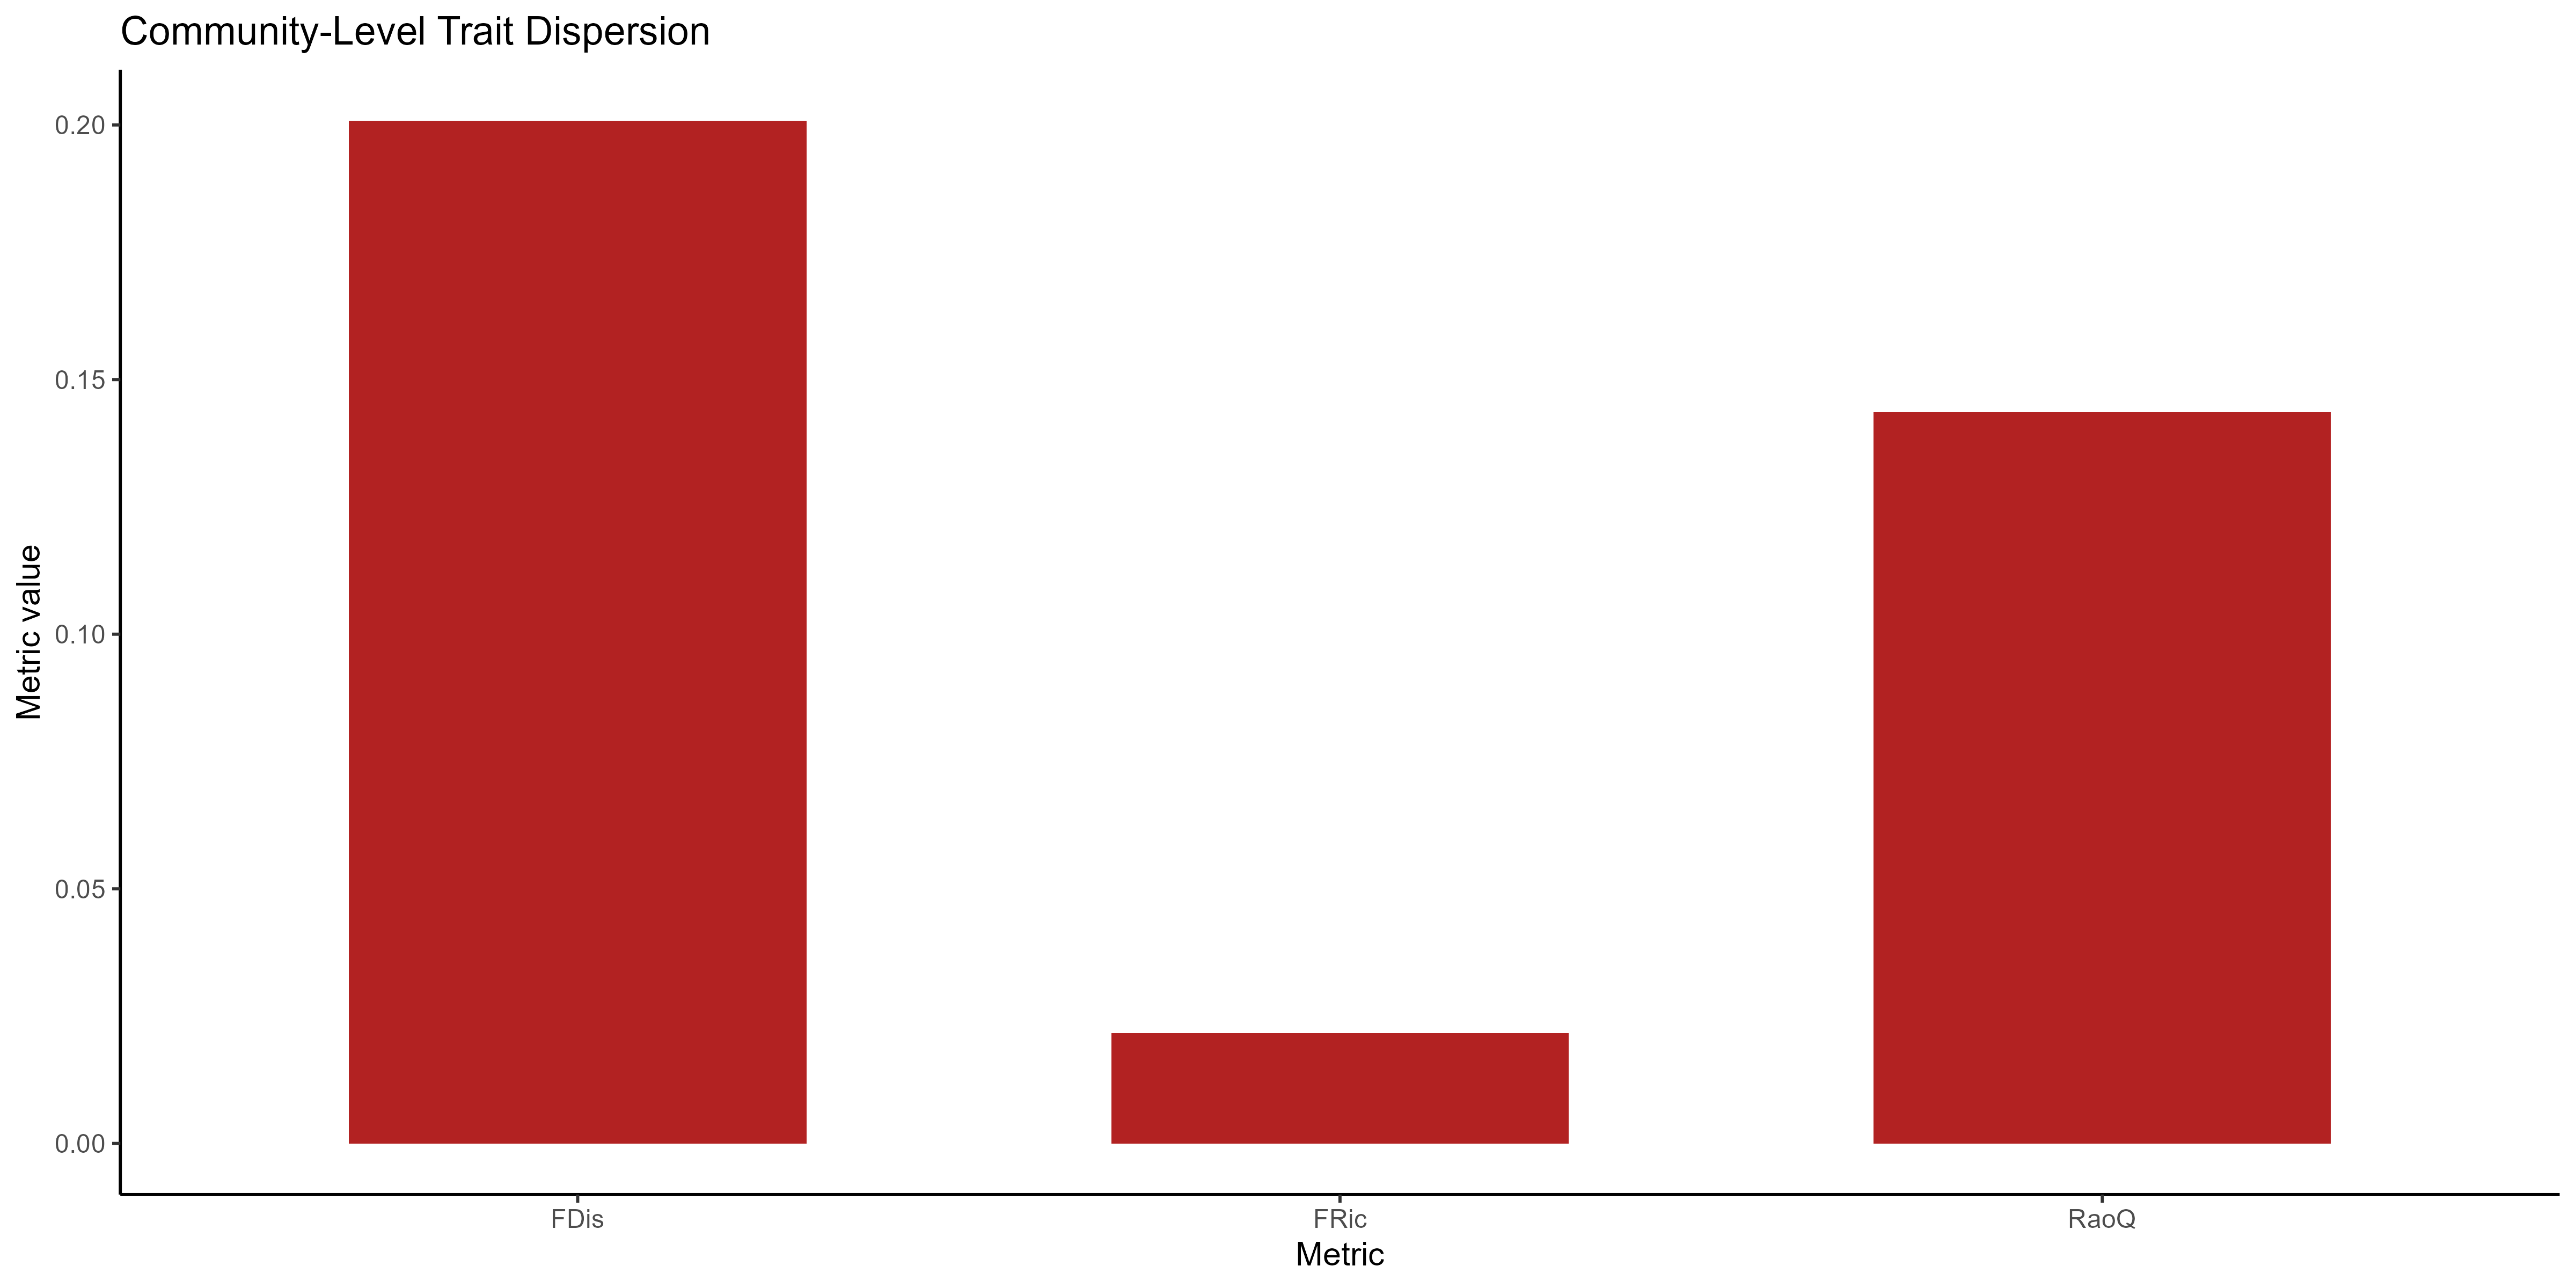
\includegraphics[width=1\linewidth]{man/figures/README-dispersion-metrics-1} \caption{Community-level functional diversity metrics.}\label{fig:dispersion-metrics}
\end{figure}

\begin{quote}
This bar chart summarises three ways of describing the community's
overall functional diversity:

\begin{itemize}
\item
  \textbf{FDis (Functional Dispersion)} - Highest value here
  (\textasciitilde0.20). Shows that, on average, species are moderately
  spread out from the community's trait centroid, meaning there is a
  fair amount of variation in trait combinations.
\item
  \textbf{FRic (Functional Richness)} - Very low value
  (\textasciitilde0.02). Indicates that the total ``volume'' of trait
  space occupied by the community is quite small --- species
  collectively use only a limited portion of the possible trait
  combinations.
\item
  \textbf{RaoQ (Rao's Quadratic Entropy)} - Intermediate value
  (\textasciitilde0.14). Measures total abundance-weighted trait
  dissimilarity. A moderate value here means that, while traits
  \textgreater\textgreater{} differ between species, much of the
  community's abundance is concentrated in species that are not
  \textgreater\textgreater{} extremely dissimilar.
\end{itemize}

\textbf{Summary}: The community has \textbf{moderate spread} of traits
(FDis), \textbf{low coverage} of the potential trait space (FRic), and
\textbf{moderate abundance-weighted diversity} (RaoQ). This suggests
that while individual species differ, the community as a whole is
functionally constrained.
\end{quote}

\hypertarget{combined-functional-workflow}{%
\subsubsection{4.6. Combined Functional
Workflow}\label{combined-functional-workflow}}

Trait-based community analyses often require multiple sequential steps:
computing per-trait similarity, calculating trait dissimilarities across
species, ordination, mapping trait space, quantifying species
centrality, and summarising community-level diversity metrics.\\
The \texttt{compute\_trait\_space()} function unifies these steps into a
single call, producing \textbf{both} per-trait similarity summaries and
community-level dispersion outputs. When run,
\texttt{compute\_trait\_space()} returns:

\begin{itemize}
\item
  \textbf{\texttt{out\$similarity}} --- \emph{Per-Trait Similarity
  Table}:\\
  Percentage similarity (0--100) for each trait column, computed as:

  \begin{itemize}
  \tightlist
  \item
    \textbf{Numeric traits} --- scaled mean pairwise similarity.
  \item
    \textbf{Categorical traits} --- proportion of identical pairs.
  \end{itemize}
\item
  \textbf{\texttt{out\$dispersion\$plots\$dend}} --- \emph{Gower
  Distance \& Hierarchical Clustering} {[}4.2{]}:\\
  Computes pairwise Gower distances across all trait types, then applies
  hierarchical clustering to reveal functional similarity structure.
\item
  \textbf{\texttt{out\$dispersion\$plots\$density\_gg}} --- \emph{Trait
  Space Mapping (PCoA)} {[}4.3{]}:\\
  Uses PCoA ordination to position species in reduced trait space;
  kernel density contours highlight clustering and gaps.
\item
  \textbf{\texttt{out\$dispersion\$plots\$centrality\_hist}} ---
  \emph{Trait Centrality} {[}4.4{]}:\\
  Shows the Euclidean distance of each species from the community
  centroid in PCoA space. Smaller distances indicate ``core'' species;
  larger distances indicate more peripheral, functionally distinct
  species.
\item
  \textbf{\texttt{out\$dispersion\$plots\$metrics\_bar}} ---
  \emph{Community-Level Trait Dispersion} {[}4.5{]}:\\
  Summarises three functional diversity metrics:

  \begin{itemize}
  \tightlist
  \item
    \textbf{FDis} --- mean distance to centroid (functional dispersion)
  \item
    \textbf{FRic} --- convex hull volume/area (functional richness)
  \item
    \textbf{RaoQ} --- abundance-weighted trait dissimilarity (Rao's
    quadratic entropy)
  \end{itemize}
\item
  \textbf{\texttt{out\$dispersion\$metrics\_df}} --- \emph{Metrics
  Table}:\\
  A tidy table of all metric values for reporting or further analysis.
\end{itemize}

\begin{Shaded}
\begin{Highlighting}[]
\CommentTok{\# res = compute\_trait\_dispersion(spp\_trait,}
\CommentTok{\#                                species\_col = 1,}
\CommentTok{\#                                k = 4,}
\CommentTok{\#                                pcoa\_dims = 2,}
\CommentTok{\#                                abundance = rep(1, nrow(spp\_trait)),  \# equal weights}
\CommentTok{\#                                kde\_n = 100,}
\CommentTok{\#                                viridis\_option = "D",}
\CommentTok{\#                                show\_plots = TRUE,                    \# combined patchwork output}
\CommentTok{\#                                show\_density\_plot = FALSE,}
\CommentTok{\#                                seed = NULL)}
\CommentTok{\# }
\CommentTok{\# str(res, max.level=1)}

\NormalTok{res }\OtherTok{=} \FunctionTok{compute\_trait\_space}\NormalTok{(}
  \AttributeTok{trait\_df =}\NormalTok{ spp\_trait,}
  \AttributeTok{species\_col =} \StringTok{"species"}\NormalTok{, }
  \AttributeTok{abundance =} \ConstantTok{NULL}\NormalTok{,}
  \AttributeTok{k =} \DecValTok{4}\NormalTok{, }
  \AttributeTok{pcoa\_dims =} \DecValTok{2}\NormalTok{, }
  \AttributeTok{show\_density\_plot =} \ConstantTok{FALSE}\NormalTok{,}
  \AttributeTok{show\_plots =} \ConstantTok{TRUE}
\NormalTok{)}
\end{Highlighting}
\end{Shaded}

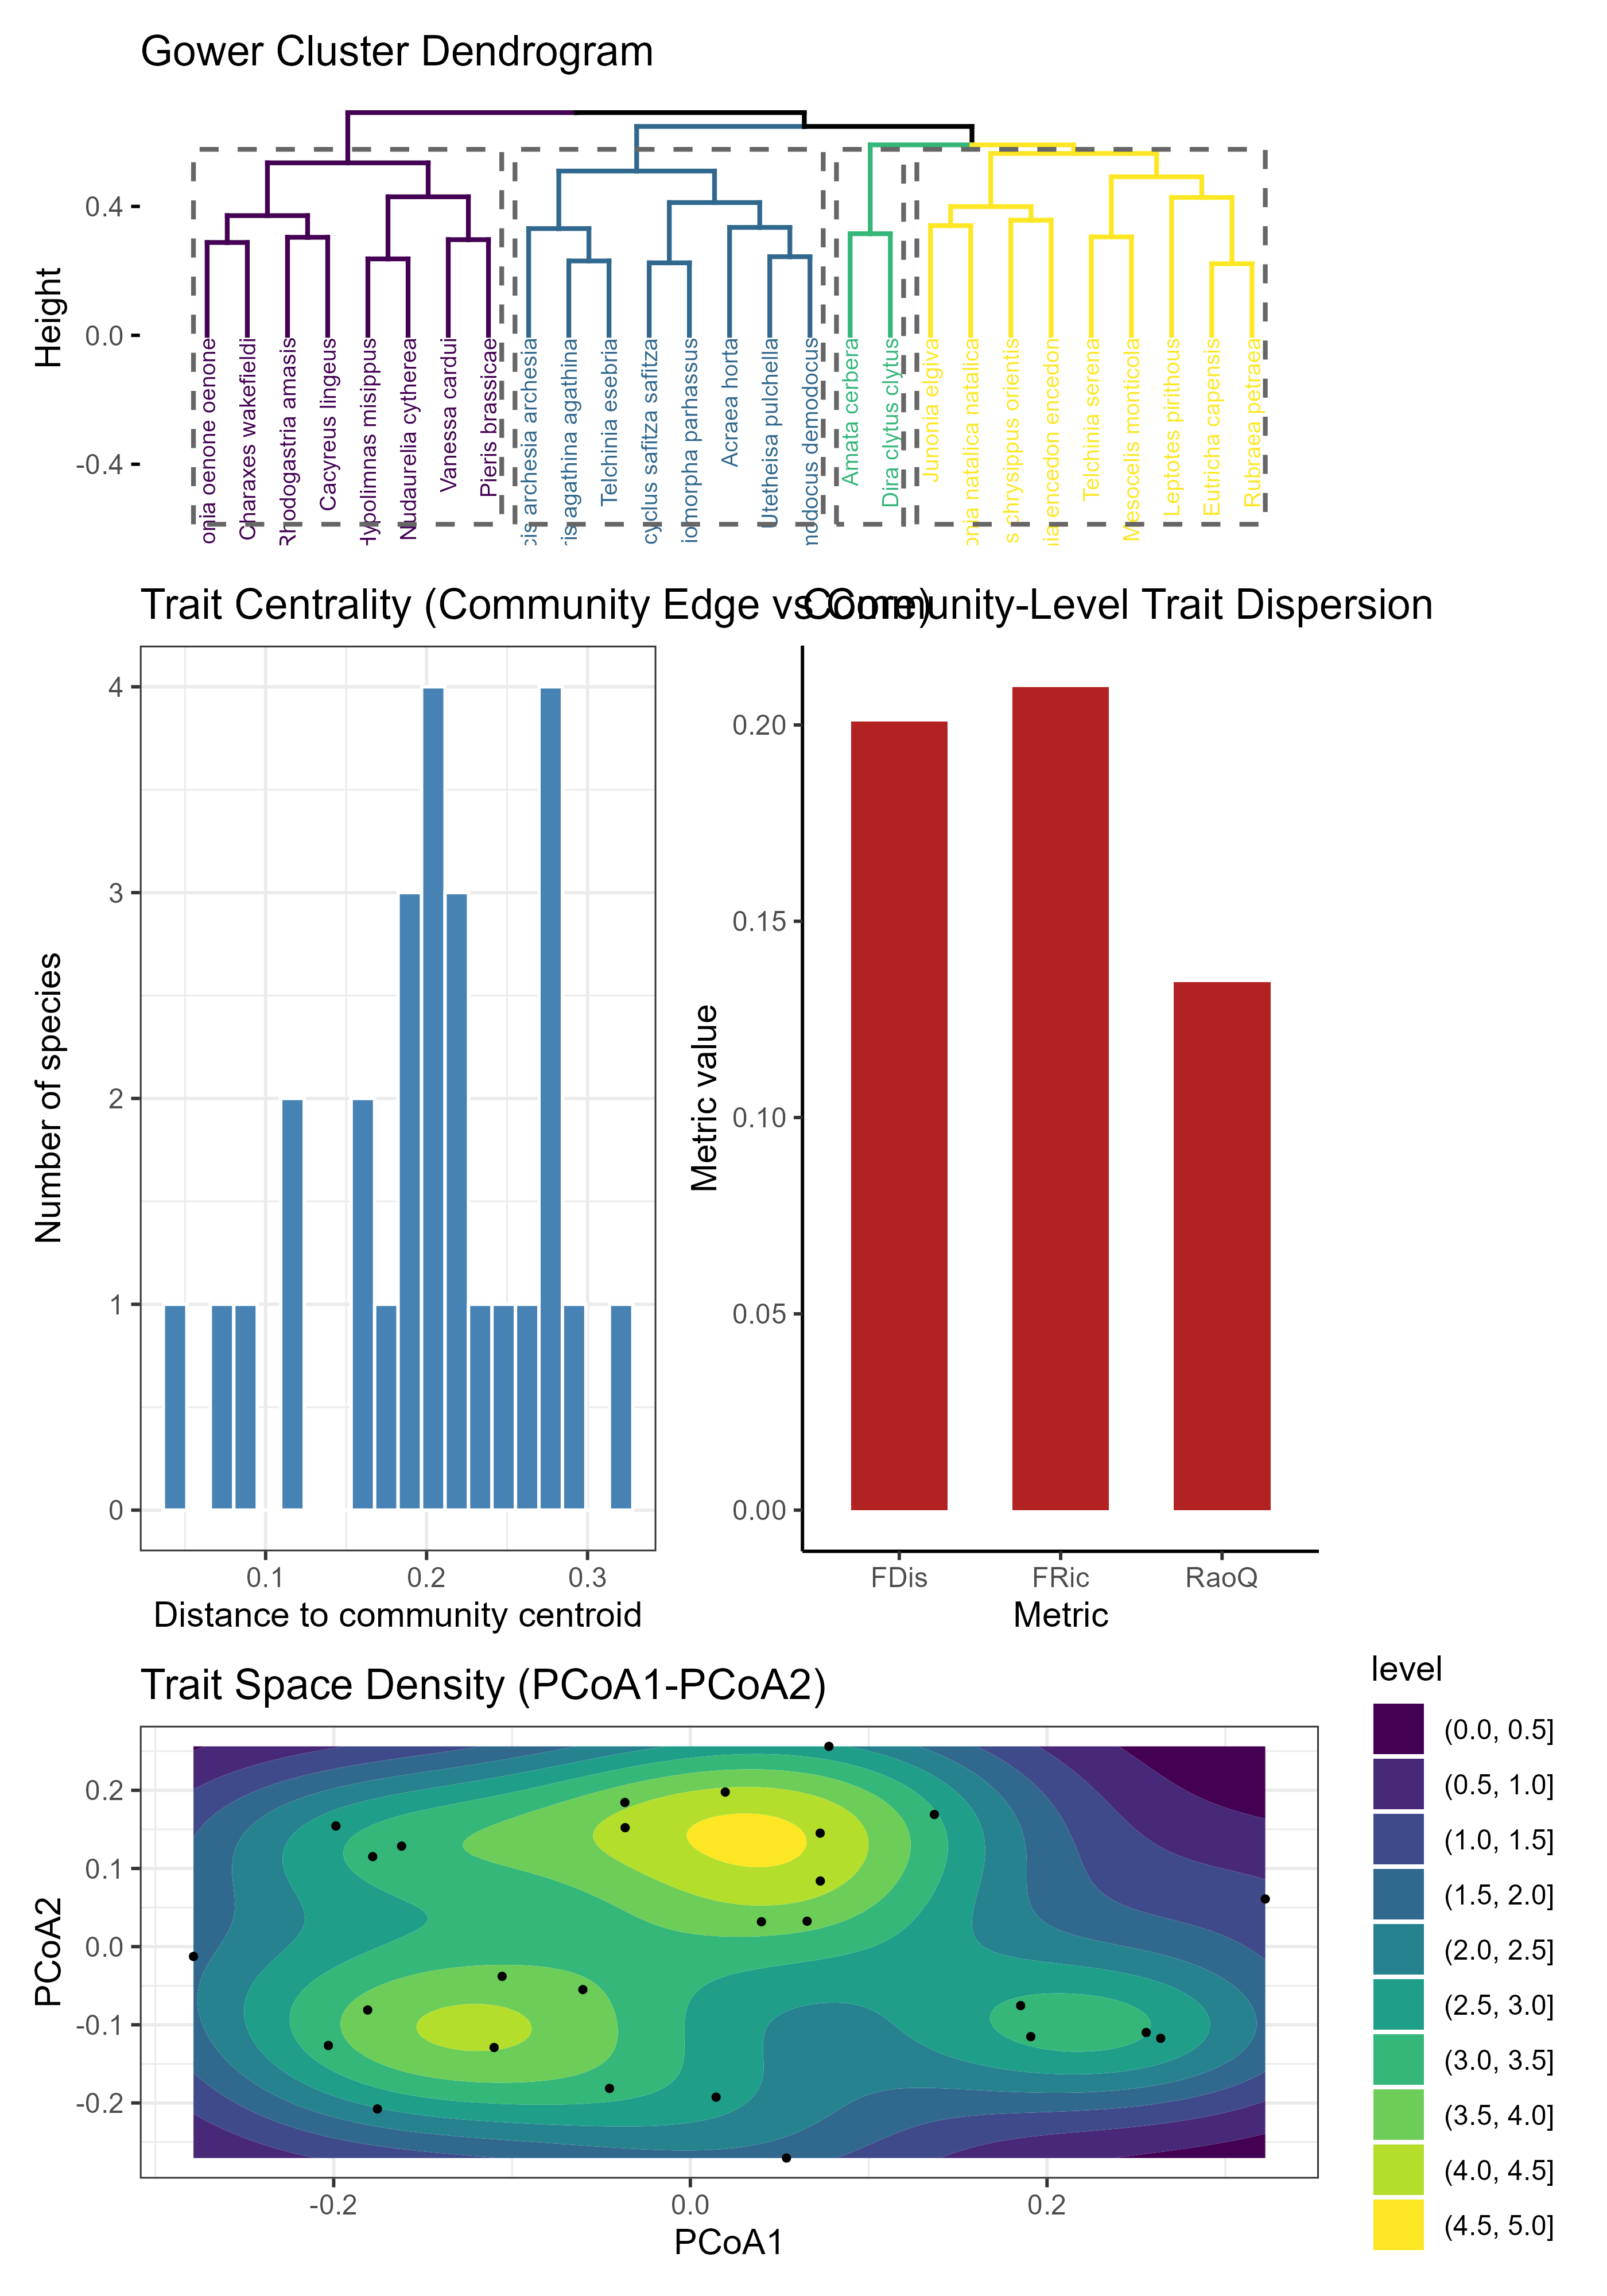
\includegraphics[width=1\linewidth]{man/figures/README-func-test-1}

\begin{Shaded}
\begin{Highlighting}[]

\FunctionTok{str}\NormalTok{(res, }\AttributeTok{max.level=}\DecValTok{1}\NormalTok{)}
\CommentTok{\#\textgreater{} List of 2}
\CommentTok{\#\textgreater{}  $ similarity:\textquotesingle{}data.frame\textquotesingle{}:  20 obs. of  2 variables:}
\CommentTok{\#\textgreater{}  $ dispersion:List of 7}

\FunctionTok{head}\NormalTok{(res}\SpecialCharTok{$}\NormalTok{similarity)}
\CommentTok{\#\textgreater{}         Trait Similarity}
\CommentTok{\#\textgreater{} 1 trait\_cont1   61.84292}
\CommentTok{\#\textgreater{} 2 trait\_cont2   63.85425}
\CommentTok{\#\textgreater{} 3 trait\_cont3   65.05900}
\CommentTok{\#\textgreater{} 4 trait\_cont4   64.09280}
\CommentTok{\#\textgreater{} 5 trait\_cont5   69.47249}
\CommentTok{\#\textgreater{} 6 trait\_cont6   62.46692}
\FunctionTok{str}\NormalTok{(res}\SpecialCharTok{$}\NormalTok{dispersion, }\AttributeTok{max.level=}\DecValTok{1}\NormalTok{)}
\CommentTok{\#\textgreater{} List of 7}
\CommentTok{\#\textgreater{}  $ distance\_matrix: num [1:27, 1:27] 0 0.304 0.358 0.394 0.413 ...}
\CommentTok{\#\textgreater{}   ..{-} attr(*, "dimnames")=List of 2}
\CommentTok{\#\textgreater{}  $ hc             :List of 7}
\CommentTok{\#\textgreater{}   ..{-} attr(*, "class")= chr "hclust"}
\CommentTok{\#\textgreater{}  $ pcoa           :List of 5}
\CommentTok{\#\textgreater{}  $ scores         :\textquotesingle{}data.frame\textquotesingle{}: 27 obs. of  3 variables:}
\CommentTok{\#\textgreater{}  $ centroid       : num [1:2] {-}3.11e{-}17 2.91e{-}17}
\CommentTok{\#\textgreater{}  $ metrics\_df     :\textquotesingle{}data.frame\textquotesingle{}: 3 obs. of  2 variables:}
\CommentTok{\#\textgreater{}  $ plots          :List of 4}
\end{Highlighting}
\end{Shaded}

\textbf{Summary}: By pairing \texttt{compute\_trait\_similarity()}
(per-trait conservation/lability) with
\texttt{compute\_trait\_dispersion()} (whole-community functional
structure), you get a complete, repeatable workflow for trait-based
invasion and coexistence studies. All plots are stored in
\texttt{res\$plots} for flexible reuse, while \texttt{res\$metrics\_df}
provides ready-to-use numerical summaries for statistical modelling.

You can also rearrange or customise the plots in \texttt{res\$plots}
using patchwork or other layout tools. For example, the code below
recreates the combined layout used when \texttt{show\_plot\ =\ TRUE},
but omits the base \texttt{filled.contour()} plot for simplicity.

\begin{Shaded}
\begin{Highlighting}[]
\FunctionTok{str}\NormalTok{(res}\SpecialCharTok{$}\NormalTok{dispersion, }\AttributeTok{max.level=}\DecValTok{1}\NormalTok{)}
\CommentTok{\#\textgreater{} List of 7}
\CommentTok{\#\textgreater{}  $ distance\_matrix: num [1:27, 1:27] 0 0.304 0.358 0.394 0.413 ...}
\CommentTok{\#\textgreater{}   ..{-} attr(*, "dimnames")=List of 2}
\CommentTok{\#\textgreater{}  $ hc             :List of 7}
\CommentTok{\#\textgreater{}   ..{-} attr(*, "class")= chr "hclust"}
\CommentTok{\#\textgreater{}  $ pcoa           :List of 5}
\CommentTok{\#\textgreater{}  $ scores         :\textquotesingle{}data.frame\textquotesingle{}: 27 obs. of  3 variables:}
\CommentTok{\#\textgreater{}  $ centroid       : num [1:2] {-}3.11e{-}17 2.91e{-}17}
\CommentTok{\#\textgreater{}  $ metrics\_df     :\textquotesingle{}data.frame\textquotesingle{}: 3 obs. of  2 variables:}
\CommentTok{\#\textgreater{}  $ plots          :List of 4}

\CommentTok{\# \# Custom combined layout without base filled.contour}
\CommentTok{\# combined = res$dispersion$plots$dend /}
\CommentTok{\#   (res$dispersion$plots$centrality\_hist | res$dispersion$plots$metrics\_bar) /}
\CommentTok{\#   res$dispersion$plots$density\_gg +}
\CommentTok{\#   patchwork::plot\_layout(heights = c(1, 2, 1))}
\CommentTok{\# }
\CommentTok{\# print(combined)  \# display in console}
\end{Highlighting}
\end{Shaded}

This flexibility means you can:

\begin{itemize}
\tightlist
\item
  Change the order or arrangement of panels
\item
  Replace individual plots with customised versions (e.g., change themes
  or colours)
\item
  Combine them with other figures in your workflow
\end{itemize}

\begin{center}\rule{0.5\linewidth}{0.5pt}\end{center}

\hypertarget{model-abundance-as-a-function-of-traits-and-environment}{%
\subsection{5. Model Abundance as a Function of Traits and
Environment}\label{model-abundance-as-a-function-of-traits-and-environment}}

To evaluate how \textbf{species functional traits, environmental
conditions}, and their \textbf{interactions} influence species
abundances, we use a \textbf{Generalized Linear Mixed Model (GLMM)}.
This framework:

\begin{itemize}
\tightlist
\item
  Quantifies the separate and combined effects of traits and
  environment.
\item
  Controls for repeated observations of the same species and sites via
  \textbf{random intercepts}, accounting for non-independence and
  spatial structure.
\item
  Is flexible enough to predict how hypothetical (invader) species might
  perform in new environments.
\end{itemize}

We use the \textbf{Tweedie} error distribution, which is well-suited to
ecological count data because it handles \textbf{overdispersion} and
\textbf{many zeros}.

\hypertarget{prepare-the-long-format-dataset}{%
\subsubsection{5.1. Prepare the long-format
dataset}\label{prepare-the-long-format-dataset}}

We first create a long-format table, where each row is a single
species-at-site observation, with all associated predictors attached:

\begin{itemize}
\tightlist
\item
  \textbf{Site metadata}: \texttt{site\_id}, spatial coordinates
  (\texttt{x}, \texttt{y})
\item
  \textbf{Species ID and count/abundance}
\item
  \textbf{Environmental predictors}: e.g., \texttt{env1}-\texttt{env10}
\item
  \textbf{Species traits}: continuous
  (\texttt{trait\_cont1}-\texttt{trait\_cont10}), categorical
  (\texttt{trait\_cat11}-\texttt{trait\_cat15}), and ordinal
  (\texttt{trait\_ord16}-\texttt{trait\_ord20})
\end{itemize}

Finally, we convert all character variables to factors so they're
correctly handled by the model.

\begin{Shaded}
\begin{Highlighting}[]
\CommentTok{\# Prepare long{-}format data}
\NormalTok{longDF }\OtherTok{=}\NormalTok{ site\_env\_spp }\SpecialCharTok{\%\textgreater{}\%}
\NormalTok{  dplyr}\SpecialCharTok{::}\FunctionTok{select}\NormalTok{(}
\NormalTok{    site\_id, x, y, species, count,           }\CommentTok{\# Metadata + response}
\NormalTok{    env1}\SpecialCharTok{:}\NormalTok{env10,                              }\CommentTok{\# Environment variables}
\NormalTok{    trait\_cont1}\SpecialCharTok{:}\NormalTok{trait\_cont10,                }\CommentTok{\# Continuous traits}
\NormalTok{    trait\_cat11}\SpecialCharTok{:}\NormalTok{trait\_cat15,                 }\CommentTok{\# Categorical traits}
\NormalTok{    trait\_ord16}\SpecialCharTok{:}\NormalTok{trait\_ord20                  }\CommentTok{\# Ordinal traits}
\NormalTok{  ) }\SpecialCharTok{\%\textgreater{}\%}
  \FunctionTok{mutate}\NormalTok{(}\FunctionTok{across}\NormalTok{(}\FunctionTok{where}\NormalTok{(is.character), as.factor))}

\FunctionTok{head}\NormalTok{(longDF)}
\CommentTok{\#\textgreater{}   site\_id     x         y                    species count     env1      env2}
\CommentTok{\#\textgreater{} 1    1026 28.75 {-}22.25004               Acraea horta    10 2.203029 0.6471631}
\CommentTok{\#\textgreater{} 2    1026 28.75 {-}22.25004              Amata cerbera     0 2.203029 0.6471631}
\CommentTok{\#\textgreater{} 3    1026 28.75 {-}22.25004   Bicyclus safitza safitza     0 2.203029 0.6471631}
\CommentTok{\#\textgreater{} 4    1026 28.75 {-}22.25004           Cacyreus lingeus     0 2.203029 0.6471631}
\CommentTok{\#\textgreater{} 5    1026 28.75 {-}22.25004        Charaxes wakefieldi     9 2.203029 0.6471631}
\CommentTok{\#\textgreater{} 6    1026 28.75 {-}22.25004 Danaus chrysippus orientis     8 2.203029 0.6471631}
\CommentTok{\#\textgreater{}         env3       env4      env5     env6      env7      env8        env9}
\CommentTok{\#\textgreater{} 1 {-}0.4910981 {-}0.7934531 0.8216381 1.545075 0.4185999 {-}1.050379 {-}0.05366469}
\CommentTok{\#\textgreater{} 2 {-}0.4910981 {-}0.7934531 0.8216381 1.545075 0.4185999 {-}1.050379 {-}0.05366469}
\CommentTok{\#\textgreater{} 3 {-}0.4910981 {-}0.7934531 0.8216381 1.545075 0.4185999 {-}1.050379 {-}0.05366469}
\CommentTok{\#\textgreater{} 4 {-}0.4910981 {-}0.7934531 0.8216381 1.545075 0.4185999 {-}1.050379 {-}0.05366469}
\CommentTok{\#\textgreater{} 5 {-}0.4910981 {-}0.7934531 0.8216381 1.545075 0.4185999 {-}1.050379 {-}0.05366469}
\CommentTok{\#\textgreater{} 6 {-}0.4910981 {-}0.7934531 0.8216381 1.545075 0.4185999 {-}1.050379 {-}0.05366469}
\CommentTok{\#\textgreater{}       env10 trait\_cont1 trait\_cont2 trait\_cont3 trait\_cont4 trait\_cont5}
\CommentTok{\#\textgreater{} 1 0.9329782   0.8296121   0.8114763 {-}0.92212702  {-}0.6841896  0.07152258}
\CommentTok{\#\textgreater{} 2 0.9329782   0.8741508  {-}0.1060607  0.49759077  {-}0.2819434 {-}0.99545407}
\CommentTok{\#\textgreater{} 3 0.9329782  {-}0.4277209   0.6720085  0.35455366   0.2912638  0.21787491}
\CommentTok{\#\textgreater{} 4 0.9329782   0.6608953   0.4751912 {-}0.65747134   0.5516467  0.67360312}
\CommentTok{\#\textgreater{} 5 0.9329782   0.2834910   0.6221103 {-}0.47782407   0.1272937  0.50304512}
\CommentTok{\#\textgreater{} 6 0.9329782   0.0381919  {-}0.2237834  0.02882587  {-}0.5325932 {-}0.09453686}
\CommentTok{\#\textgreater{}   trait\_cont6 trait\_cont7 trait\_cont8 trait\_cont9 trait\_cont10 trait\_cat11}
\CommentTok{\#\textgreater{} 1   0.1596418  0.20353247  {-}0.4245005  0.14927467 {-}0.577216122     wetland}
\CommentTok{\#\textgreater{} 2   0.6428078 {-}0.60601102  {-}0.6106477 {-}0.29329924  0.099240827      forest}
\CommentTok{\#\textgreater{} 3  {-}0.7725628  0.07047322   0.5682188  0.09485216 {-}0.036037103     wetland}
\CommentTok{\#\textgreater{} 4   0.5290155 {-}0.64088852  {-}0.7422557  0.78543719 {-}0.681060291     wetland}
\CommentTok{\#\textgreater{} 5   0.2472269 {-}0.09622701  {-}0.7418214 {-}0.02001886 {-}0.700842010      forest}
\CommentTok{\#\textgreater{} 6  {-}0.7031068 {-}0.36589330  {-}0.8554938 {-}0.65673577 {-}0.001454239   grassland}
\CommentTok{\#\textgreater{}   trait\_cat12  trait\_cat13 trait\_cat14 trait\_cat15 trait\_ord16 trait\_ord17}
\CommentTok{\#\textgreater{} 1     diurnal    bivoltine detritivore   migratory           4           1}
\CommentTok{\#\textgreater{} 2   nocturnal multivoltine detritivore    resident           1           4}
\CommentTok{\#\textgreater{} 3     diurnal   univoltine  generalist    resident           4           4}
\CommentTok{\#\textgreater{} 4   nocturnal multivoltine nectarivore   migratory           3           3}
\CommentTok{\#\textgreater{} 5   nocturnal    bivoltine  generalist   migratory           4           2}
\CommentTok{\#\textgreater{} 6     diurnal   univoltine detritivore   migratory           1           4}
\CommentTok{\#\textgreater{}   trait\_bin18 trait\_bin19 trait\_ord20}
\CommentTok{\#\textgreater{} 1           1           1      medium}
\CommentTok{\#\textgreater{} 2           1           0       large}
\CommentTok{\#\textgreater{} 3           1           1      medium}
\CommentTok{\#\textgreater{} 4           0           0      medium}
\CommentTok{\#\textgreater{} 5           1           0      medium}
\CommentTok{\#\textgreater{} 6           1           1      medium}

\CommentTok{\# \# Use \textasciigrave{}grid\_obs\textasciigrave{} from \textasciigrave{}dissmapr\textasciigrave{} imports instead}
\CommentTok{\# longDF = grid\_obs \%\textgreater{}\%}
\CommentTok{\#   mutate(site\_id = as.character(site\_id)) \%\textgreater{}\%}
\CommentTok{\#   left\_join(site\_env \%\textgreater{}\% dplyr::select({-}x, {-}y) \%\textgreater{}\% }
\CommentTok{\#               mutate(site\_id = as.character(site\_id)), by = "site\_id") \%\textgreater{}\%}
\CommentTok{\#   left\_join(spp\_trait \%\textgreater{}\% }
\CommentTok{\#               mutate(species = as.character(species)), by = "species") \%\textgreater{}\%}
\CommentTok{\#   mutate(across(where(is.character), as.factor))  \# Ensure all character fields are treated as factors}
\CommentTok{\# \# head(longDF)}
\end{Highlighting}
\end{Shaded}

\hypertarget{build-the-model-formula}{%
\subsubsection{5.2. Build the model
formula}\label{build-the-model-formula}}

We use \texttt{build\_glmm\_formula()} to \textbf{automatically detect}
trait and environmental predictor columns based on naming conventions
(prefixes like ``\texttt{trait\_}'' or ``\texttt{env\_}'') or by
excluding known metadata columns (\texttt{site\_id}, \texttt{x},
\texttt{y}, \texttt{species}, \texttt{count}).

The function then:

\begin{itemize}
\tightlist
\item
  \textbf{Generates main effect terms} for all detected traits and all
  detected environment variables.
\item
  \textbf{Optionally expands} these into \textbf{all pairwise trait ×
  environment interactions} (e.g., \texttt{trait\_cont1:env3}),
  capturing environment-dependent trait effects.
\item
  \textbf{Appends random intercepts} for the grouping variables
  specified in \texttt{random\_effects} (default:
  ``\texttt{(1\ \textbar{}\ species)}'' and
  ``\texttt{(1\ \textbar{}\ site\_id)}'').
\item
  \textbf{Returns a valid R formula object} ready for model fitting.
\end{itemize}

This automatic approach ensures that the model always reflects the full
trait--environment structure without hard-coding variable names.

\begin{Shaded}
\begin{Highlighting}[]
\CommentTok{\# Automatically build the GLMM formula}
\NormalTok{fml }\OtherTok{=} \FunctionTok{build\_glmm\_formula}\NormalTok{(}
  \AttributeTok{data                 =}\NormalTok{ longDF,}
  \AttributeTok{response             =} \StringTok{"count"}\NormalTok{,            }\CommentTok{\# Response variable}
  \AttributeTok{species\_col          =} \StringTok{"species"}\NormalTok{,          }\CommentTok{\# Random effect grouping}
  \AttributeTok{site\_col             =} \StringTok{"site\_id"}\NormalTok{,          }\CommentTok{\# Random effect grouping}
  \AttributeTok{include\_interactions =} \ConstantTok{TRUE}\NormalTok{,               }\CommentTok{\# Add all trait × environment terms}
  \AttributeTok{random\_effects       =} \FunctionTok{c}\NormalTok{(}\StringTok{"(1 | species)"}\NormalTok{, }\StringTok{"(1 | site\_id)"}\NormalTok{)}
\NormalTok{)}

\NormalTok{fml}
\CommentTok{\#\textgreater{} count \textasciitilde{} trait\_cont1 + trait\_cont2 + trait\_cont3 + trait\_cont4 + }
\CommentTok{\#\textgreater{}     trait\_cont5 + trait\_cont6 + trait\_cont7 + trait\_cont8 + trait\_cont9 + }
\CommentTok{\#\textgreater{}     trait\_cont10 + trait\_cat11 + trait\_cat12 + trait\_cat13 + }
\CommentTok{\#\textgreater{}     trait\_cat14 + trait\_cat15 + trait\_ord16 + trait\_ord17 + trait\_bin18 + }
\CommentTok{\#\textgreater{}     trait\_bin19 + trait\_ord20 + env1 + env2 + env3 + env4 + env5 + }
\CommentTok{\#\textgreater{}     env6 + env7 + env8 + env9 + env10 + (trait\_cont1 + trait\_cont2 + }
\CommentTok{\#\textgreater{}     trait\_cont3 + trait\_cont4 + trait\_cont5 + trait\_cont6 + trait\_cont7 + }
\CommentTok{\#\textgreater{}     trait\_cont8 + trait\_cont9 + trait\_cont10 + trait\_cat11 + }
\CommentTok{\#\textgreater{}     trait\_cat12 + trait\_cat13 + trait\_cat14 + trait\_cat15 + trait\_ord16 + }
\CommentTok{\#\textgreater{}     trait\_ord17 + trait\_bin18 + trait\_bin19 + trait\_ord20):(env1 + }
\CommentTok{\#\textgreater{}     env2 + env3 + env4 + env5 + env6 + env7 + env8 + env9 + env10) + }
\CommentTok{\#\textgreater{}     (1 | species) + (1 | site\_id)}
\CommentTok{\#\textgreater{} \textless{}environment: 0x000001d0b1526078\textgreater{}}
\CommentTok{\# Example output:}
\CommentTok{\# count \textasciitilde{} trait\_cont1 + trait\_cont2 + ... + env1 + env2 + ... +}
\CommentTok{\#         (trait\_cont1 + ... + trait\_cat15):(env1 + ... + env10) +}
\CommentTok{\#         (1 | species) + (1 | site\_id)}
\end{Highlighting}
\end{Shaded}

\hypertarget{fit-the-glmm}{%
\subsubsection{5.3. Fit the GLMM}\label{fit-the-glmm}}

We fit the model using \texttt{glmmTMB::glmmTMB()}, which supports a
wide range of distributions and correlation structures.

In this case:

\begin{itemize}
\tightlist
\item
  \textbf{Family}: \texttt{tweedie(link\ =\ "log")}

  \begin{itemize}
  \tightlist
  \item
    Handles overdispersed count data and zero-inflation without
    requiring a separate zero-inflated component.
  \item
    The \textbf{log link} models multiplicative effects of predictors on
    expected abundance.
  \end{itemize}
\item
  \textbf{Data}: The prepared long-format table (\texttt{longDF}).
\item
  \textbf{Formula}: The formula, automatically generated \texttt{fml}
  from \texttt{build\_glmm\_formula()} or user customised.
\end{itemize}

The model is fit via maximum likelihood, estimating both fixed-effect
coefficients (for traits, environments, and their interactions) and
variance components for the random effects.

\begin{Shaded}
\begin{Highlighting}[]
\CommentTok{\# Fit Tweedie GLMM}
\FunctionTok{set.seed}\NormalTok{(}\DecValTok{123}\NormalTok{)}
\NormalTok{mod }\OtherTok{=}\NormalTok{ glmmTMB}\SpecialCharTok{::}\FunctionTok{glmmTMB}\NormalTok{(}
  \AttributeTok{formula =}\NormalTok{ fml,}
  \AttributeTok{data    =}\NormalTok{ longDF,}
  \AttributeTok{family  =}\NormalTok{ glmmTMB}\SpecialCharTok{::}\FunctionTok{tweedie}\NormalTok{(}\AttributeTok{link =} \StringTok{"log"}\NormalTok{)}
\NormalTok{)}

\FunctionTok{summary}\NormalTok{(mod)}
\CommentTok{\#\textgreater{}  Family: tweedie  ( log )}
\CommentTok{\#\textgreater{} Formula:          }
\CommentTok{\#\textgreater{} count \textasciitilde{} trait\_cont1 + trait\_cont2 + trait\_cont3 + trait\_cont4 +  }
\CommentTok{\#\textgreater{}     trait\_cont5 + trait\_cont6 + trait\_cont7 + trait\_cont8 + trait\_cont9 +  }
\CommentTok{\#\textgreater{}     trait\_cont10 + trait\_cat11 + trait\_cat12 + trait\_cat13 +  }
\CommentTok{\#\textgreater{}     trait\_cat14 + trait\_cat15 + trait\_ord16 + trait\_ord17 + trait\_bin18 +  }
\CommentTok{\#\textgreater{}     trait\_bin19 + trait\_ord20 + env1 + env2 + env3 + env4 + env5 +  }
\CommentTok{\#\textgreater{}     env6 + env7 + env8 + env9 + env10 + (trait\_cont1 + trait\_cont2 +  }
\CommentTok{\#\textgreater{}     trait\_cont3 + trait\_cont4 + trait\_cont5 + trait\_cont6 + trait\_cont7 +  }
\CommentTok{\#\textgreater{}     trait\_cont8 + trait\_cont9 + trait\_cont10 + trait\_cat11 +  }
\CommentTok{\#\textgreater{}     trait\_cat12 + trait\_cat13 + trait\_cat14 + trait\_cat15 + trait\_ord16 +  }
\CommentTok{\#\textgreater{}     trait\_ord17 + trait\_bin18 + trait\_bin19 + trait\_ord20):(env1 +  }
\CommentTok{\#\textgreater{}     env2 + env3 + env4 + env5 + env6 + env7 + env8 + env9 + env10) +  }
\CommentTok{\#\textgreater{}     (1 | species) + (1 | site\_id)}
\CommentTok{\#\textgreater{} Data: longDF}
\CommentTok{\#\textgreater{} }
\CommentTok{\#\textgreater{}       AIC       BIC    logLik {-}2*log(L)  df.resid }
\CommentTok{\#\textgreater{}   38196.0   40239.4  {-}18819.0   37638.0     10926 }
\CommentTok{\#\textgreater{} }
\CommentTok{\#\textgreater{} Random effects:}
\CommentTok{\#\textgreater{} }
\CommentTok{\#\textgreater{} Conditional model:}
\CommentTok{\#\textgreater{}  Groups  Name        Variance  Std.Dev.}
\CommentTok{\#\textgreater{}  species (Intercept) 0.0007666 0.02769 }
\CommentTok{\#\textgreater{}  site\_id (Intercept) 0.0067449 0.08213 }
\CommentTok{\#\textgreater{} Number of obs: 11205, groups:  species, 27; site\_id, 415}
\CommentTok{\#\textgreater{} }
\CommentTok{\#\textgreater{} Dispersion parameter for tweedie family (): 7.98 }
\CommentTok{\#\textgreater{} }
\CommentTok{\#\textgreater{} Conditional model:}
\CommentTok{\#\textgreater{}                                 Estimate Std. Error z value Pr(\textgreater{}|z|)    }
\CommentTok{\#\textgreater{} (Intercept)                    1.4704424  0.2628156   5.595 2.21e{-}08 ***}
\CommentTok{\#\textgreater{} trait\_cont1                   {-}0.5101186  0.1596020  {-}3.196 0.001393 ** }
\CommentTok{\#\textgreater{} trait\_cont2                   {-}0.2327202  0.0678723  {-}3.429 0.000606 ***}
\CommentTok{\#\textgreater{} trait\_cont3                   {-}0.0341002  0.1094644  {-}0.312 0.755407    }
\CommentTok{\#\textgreater{} trait\_cont4                    0.0130361  0.0849067   0.154 0.877977    }
\CommentTok{\#\textgreater{} trait\_cont5                    0.0729463  0.0994374   0.734 0.463199    }
\CommentTok{\#\textgreater{} trait\_cont6                    0.0968116  0.1181499   0.819 0.412560    }
\CommentTok{\#\textgreater{} trait\_cont7                   {-}0.0688003  0.0874939  {-}0.786 0.431666    }
\CommentTok{\#\textgreater{} trait\_cont8                    0.1176131  0.1168984   1.006 0.314361    }
\CommentTok{\#\textgreater{} trait\_cont9                   {-}0.0103170  0.0824478  {-}0.125 0.900418    }
\CommentTok{\#\textgreater{} trait\_cont10                   0.1304327  0.0805313   1.620 0.105307    }
\CommentTok{\#\textgreater{} trait\_cat11grassland           0.0306508  0.1759612   0.174 0.861716    }
\CommentTok{\#\textgreater{} trait\_cat11wetland            {-}0.1600557  0.2324683  {-}0.689 0.491134    }
\CommentTok{\#\textgreater{} trait\_cat12nocturnal          {-}0.2304255  0.1110776  {-}2.074 0.038037 *  }
\CommentTok{\#\textgreater{} trait\_cat13multivoltine       {-}0.0010464  0.0923656  {-}0.011 0.990961    }
\CommentTok{\#\textgreater{} trait\_cat13univoltine         {-}0.2102297  0.1253302  {-}1.677 0.093463 .  }
\CommentTok{\#\textgreater{} trait\_cat14generalist          0.0071383  0.2479466   0.029 0.977032    }
\CommentTok{\#\textgreater{} trait\_cat14nectarivore         0.2505427  0.1645857   1.522 0.127943    }
\CommentTok{\#\textgreater{} trait\_cat15resident           {-}0.0296779  0.1293586  {-}0.229 0.818540    }
\CommentTok{\#\textgreater{} trait\_ord16                    0.0100260  0.0466039   0.215 0.829665    }
\CommentTok{\#\textgreater{} trait\_ord17                   {-}0.0374465  0.0314953  {-}1.189 0.234457    }
\CommentTok{\#\textgreater{} trait\_bin18                    0.0873029  0.0915280   0.954 0.340165    }
\CommentTok{\#\textgreater{} trait\_bin19                    0.0315366  0.1155415   0.273 0.784895    }
\CommentTok{\#\textgreater{} trait\_ord20medium              0.1233020  0.2515604   0.490 0.624029    }
\CommentTok{\#\textgreater{} trait\_ord20small              {-}0.1603479  0.1475234  {-}1.087 0.277067    }
\CommentTok{\#\textgreater{} env1                           0.5422358  0.5433334   0.998 0.318289    }
\CommentTok{\#\textgreater{} env2                          {-}1.0286903  0.5629959  {-}1.827 0.067674 .  }
\CommentTok{\#\textgreater{} env3                          {-}0.4640513  0.8122554  {-}0.571 0.567788    }
\CommentTok{\#\textgreater{} env4                           0.5304439  0.6134961   0.865 0.387245    }
\CommentTok{\#\textgreater{} env5                           0.4719702  0.6761339   0.698 0.485151    }
\CommentTok{\#\textgreater{} env6                           0.3931038  0.6982169   0.563 0.573427    }
\CommentTok{\#\textgreater{} env7                           0.3775495  0.9974476   0.379 0.705048    }
\CommentTok{\#\textgreater{} env8                          {-}0.2439993  1.1758269  {-}0.208 0.835609    }
\CommentTok{\#\textgreater{} env9                          {-}0.6138702  1.2123491  {-}0.506 0.612613    }
\CommentTok{\#\textgreater{} env10                         {-}0.4518295  1.2848177  {-}0.352 0.725087    }
\CommentTok{\#\textgreater{} trait\_cont1:env1               0.4542883  0.3307548   1.373 0.169600    }
\CommentTok{\#\textgreater{} trait\_cont1:env2              {-}0.1657942  0.3429966  {-}0.483 0.628833    }
\CommentTok{\#\textgreater{} trait\_cont1:env3              {-}0.0672174  0.4913060  {-}0.137 0.891178    }
\CommentTok{\#\textgreater{} trait\_cont1:env4               0.3310830  0.3695503   0.896 0.370302    }
\CommentTok{\#\textgreater{} trait\_cont1:env5              {-}0.0086909  0.4129877  {-}0.021 0.983211    }
\CommentTok{\#\textgreater{} trait\_cont1:env6              {-}0.0522244  0.4194517  {-}0.125 0.900914    }
\CommentTok{\#\textgreater{} trait\_cont1:env7              {-}0.2542360  0.6089449  {-}0.418 0.676311    }
\CommentTok{\#\textgreater{} trait\_cont1:env8              {-}0.1987654  0.7093235  {-}0.280 0.779310    }
\CommentTok{\#\textgreater{} trait\_cont1:env9               0.0132204  0.7344460   0.018 0.985638    }
\CommentTok{\#\textgreater{} trait\_cont1:env10              0.2976046  0.7825323   0.380 0.703716    }
\CommentTok{\#\textgreater{} trait\_cont2:env1               0.1224603  0.1401736   0.874 0.382318    }
\CommentTok{\#\textgreater{} trait\_cont2:env2               0.1257619  0.1457562   0.863 0.388234    }
\CommentTok{\#\textgreater{} trait\_cont2:env3               0.0510393  0.2097336   0.243 0.807732    }
\CommentTok{\#\textgreater{} trait\_cont2:env4              {-}0.0545704  0.1554956  {-}0.351 0.725630    }
\CommentTok{\#\textgreater{} trait\_cont2:env5              {-}0.0523391  0.1758109  {-}0.298 0.765931    }
\CommentTok{\#\textgreater{} trait\_cont2:env6              {-}0.0236931  0.1776132  {-}0.133 0.893879    }
\CommentTok{\#\textgreater{} trait\_cont2:env7               0.0193329  0.2592569   0.075 0.940556    }
\CommentTok{\#\textgreater{} trait\_cont2:env8              {-}0.0035217  0.3032631  {-}0.012 0.990735    }
\CommentTok{\#\textgreater{} trait\_cont2:env9               0.0114218  0.3123773   0.037 0.970833    }
\CommentTok{\#\textgreater{} trait\_cont2:env10             {-}0.1187163  0.3333231  {-}0.356 0.721721    }
\CommentTok{\#\textgreater{} trait\_cont3:env1               0.0224383  0.2268712   0.099 0.921215    }
\CommentTok{\#\textgreater{} trait\_cont3:env2               0.0197380  0.2373843   0.083 0.933734    }
\CommentTok{\#\textgreater{} trait\_cont3:env3               0.1063384  0.3360710   0.316 0.751686    }
\CommentTok{\#\textgreater{} trait\_cont3:env4               0.2250068  0.2545347   0.884 0.376700    }
\CommentTok{\#\textgreater{} trait\_cont3:env5               0.0438643  0.2815770   0.156 0.876206    }
\CommentTok{\#\textgreater{} trait\_cont3:env6               0.0931172  0.2868353   0.325 0.745456    }
\CommentTok{\#\textgreater{} trait\_cont3:env7              {-}0.3698838  0.4171191  {-}0.887 0.375209    }
\CommentTok{\#\textgreater{} trait\_cont3:env8              {-}0.2242540  0.4868664  {-}0.461 0.645081    }
\CommentTok{\#\textgreater{} trait\_cont3:env9              {-}0.1435396  0.5033282  {-}0.285 0.775506    }
\CommentTok{\#\textgreater{} trait\_cont3:env10              0.1991328  0.5354910   0.372 0.709990    }
\CommentTok{\#\textgreater{} trait\_cont4:env1               0.0662273  0.1761968   0.376 0.707013    }
\CommentTok{\#\textgreater{} trait\_cont4:env2               0.0482631  0.1848803   0.261 0.794054    }
\CommentTok{\#\textgreater{} trait\_cont4:env3               0.0475713  0.2618060   0.182 0.855815    }
\CommentTok{\#\textgreater{} trait\_cont4:env4               0.0558466  0.1984742   0.281 0.778419    }
\CommentTok{\#\textgreater{} trait\_cont4:env5              {-}0.0079881  0.2180135  {-}0.037 0.970772    }
\CommentTok{\#\textgreater{} trait\_cont4:env6               0.1322373  0.2240845   0.590 0.555109    }
\CommentTok{\#\textgreater{} trait\_cont4:env7               0.0030004  0.3240575   0.009 0.992613    }
\CommentTok{\#\textgreater{} trait\_cont4:env8              {-}0.0559403  0.3797565  {-}0.147 0.882891    }
\CommentTok{\#\textgreater{} trait\_cont4:env9              {-}0.0373883  0.3919177  {-}0.095 0.923998    }
\CommentTok{\#\textgreater{} trait\_cont4:env10             {-}0.2119408  0.4155868  {-}0.510 0.610066    }
\CommentTok{\#\textgreater{} trait\_cont5:env1              {-}0.3157162  0.2076197  {-}1.521 0.128348    }
\CommentTok{\#\textgreater{} trait\_cont5:env2              {-}0.0020636  0.2157308  {-}0.010 0.992368    }
\CommentTok{\#\textgreater{} trait\_cont5:env3              {-}0.0658514  0.3077739  {-}0.214 0.830578    }
\CommentTok{\#\textgreater{} trait\_cont5:env4               0.0134922  0.2354324   0.057 0.954300    }
\CommentTok{\#\textgreater{} trait\_cont5:env5               0.0261295  0.2553548   0.102 0.918498    }
\CommentTok{\#\textgreater{} trait\_cont5:env6               0.2519034  0.2647715   0.951 0.341402    }
\CommentTok{\#\textgreater{} trait\_cont5:env7              {-}0.4533944  0.3789051  {-}1.197 0.231466    }
\CommentTok{\#\textgreater{} trait\_cont5:env8               0.0661443  0.4466947   0.148 0.882284    }
\CommentTok{\#\textgreater{} trait\_cont5:env9               0.0510576  0.4586971   0.111 0.911371    }
\CommentTok{\#\textgreater{} trait\_cont5:env10              0.5789141  0.4873776   1.188 0.234907    }
\CommentTok{\#\textgreater{} trait\_cont6:env1              {-}0.1881089  0.2447584  {-}0.769 0.442161    }
\CommentTok{\#\textgreater{} trait\_cont6:env2               0.1347617  0.2537602   0.531 0.595378    }
\CommentTok{\#\textgreater{} trait\_cont6:env3               0.1762242  0.3631814   0.485 0.627518    }
\CommentTok{\#\textgreater{} trait\_cont6:env4              {-}0.1655427  0.2731632  {-}0.606 0.544501    }
\CommentTok{\#\textgreater{} trait\_cont6:env5              {-}0.0584509  0.3052173  {-}0.192 0.848129    }
\CommentTok{\#\textgreater{} trait\_cont6:env6               0.1809909  0.3105673   0.583 0.560045    }
\CommentTok{\#\textgreater{} trait\_cont6:env7               0.0136916  0.4483815   0.031 0.975640    }
\CommentTok{\#\textgreater{} trait\_cont6:env8              {-}0.0287384  0.5247439  {-}0.055 0.956324    }
\CommentTok{\#\textgreater{} trait\_cont6:env9               0.1670829  0.5425820   0.308 0.758128    }
\CommentTok{\#\textgreater{} trait\_cont6:env10             {-}0.0216889  0.5775002  {-}0.038 0.970041    }
\CommentTok{\#\textgreater{} trait\_cont7:env1               0.0117718  0.1832154   0.064 0.948770    }
\CommentTok{\#\textgreater{} trait\_cont7:env2              {-}0.2494385  0.1908231  {-}1.307 0.191155    }
\CommentTok{\#\textgreater{} trait\_cont7:env3              {-}0.2403364  0.2736175  {-}0.878 0.379745    }
\CommentTok{\#\textgreater{} trait\_cont7:env4               0.1897891  0.2073779   0.915 0.360095    }
\CommentTok{\#\textgreater{} trait\_cont7:env5               0.0307101  0.2285526   0.134 0.893112    }
\CommentTok{\#\textgreater{} trait\_cont7:env6               0.2824628  0.2343997   1.205 0.228185    }
\CommentTok{\#\textgreater{} trait\_cont7:env7              {-}0.1028858  0.3374557  {-}0.305 0.760452    }
\CommentTok{\#\textgreater{} trait\_cont7:env8              {-}0.0941266  0.3973214  {-}0.237 0.812732    }
\CommentTok{\#\textgreater{} trait\_cont7:env9               0.0188233  0.4101149   0.046 0.963392    }
\CommentTok{\#\textgreater{} trait\_cont7:env10              0.0654068  0.4330113   0.151 0.879936    }
\CommentTok{\#\textgreater{} trait\_cont8:env1              {-}0.1719497  0.2425198  {-}0.709 0.478316    }
\CommentTok{\#\textgreater{} trait\_cont8:env2              {-}0.2490949  0.2505595  {-}0.994 0.320148    }
\CommentTok{\#\textgreater{} trait\_cont8:env3              {-}0.1298487  0.3597634  {-}0.361 0.718153    }
\CommentTok{\#\textgreater{} trait\_cont8:env4              {-}0.0541162  0.2704139  {-}0.200 0.841384    }
\CommentTok{\#\textgreater{} trait\_cont8:env5               0.1029516  0.3019067   0.341 0.733100    }
\CommentTok{\#\textgreater{} trait\_cont8:env6               0.2066006  0.3083429   0.670 0.502835    }
\CommentTok{\#\textgreater{} trait\_cont8:env7               0.0301432  0.4444334   0.068 0.945926    }
\CommentTok{\#\textgreater{} trait\_cont8:env8               0.0388618  0.5189531   0.075 0.940306    }
\CommentTok{\#\textgreater{} trait\_cont8:env9               0.0657501  0.5389646   0.122 0.902904    }
\CommentTok{\#\textgreater{} trait\_cont8:env10              0.1524384  0.5715950   0.267 0.789708    }
\CommentTok{\#\textgreater{} trait\_cont9:env1               0.0491704  0.1729237   0.284 0.776144    }
\CommentTok{\#\textgreater{} trait\_cont9:env2              {-}0.1516373  0.1800992  {-}0.842 0.399807    }
\CommentTok{\#\textgreater{} trait\_cont9:env3               0.0404439  0.2559539   0.158 0.874447    }
\CommentTok{\#\textgreater{} trait\_cont9:env4               0.1468507  0.1926070   0.762 0.445799    }
\CommentTok{\#\textgreater{} trait\_cont9:env5               0.1078422  0.2144027   0.503 0.614972    }
\CommentTok{\#\textgreater{} trait\_cont9:env6               0.1373539  0.2175442   0.631 0.527790    }
\CommentTok{\#\textgreater{} trait\_cont9:env7               0.0709711  0.3175835   0.223 0.823168    }
\CommentTok{\#\textgreater{} trait\_cont9:env8              {-}0.1044847  0.3705180  {-}0.282 0.777946    }
\CommentTok{\#\textgreater{} trait\_cont9:env9              {-}0.0241682  0.3826458  {-}0.063 0.949638    }
\CommentTok{\#\textgreater{} trait\_cont9:env10             {-}0.0707903  0.4081366  {-}0.173 0.862300    }
\CommentTok{\#\textgreater{} trait\_cont10:env1             {-}0.0161651  0.1675005  {-}0.097 0.923117    }
\CommentTok{\#\textgreater{} trait\_cont10:env2             {-}0.0123918  0.1748189  {-}0.071 0.943490    }
\CommentTok{\#\textgreater{} trait\_cont10:env3             {-}0.1351959  0.2499217  {-}0.541 0.588540    }
\CommentTok{\#\textgreater{} trait\_cont10:env4             {-}0.0179706  0.1863072  {-}0.096 0.923158    }
\CommentTok{\#\textgreater{} trait\_cont10:env5             {-}0.0960179  0.2093890  {-}0.459 0.646548    }
\CommentTok{\#\textgreater{} trait\_cont10:env6              0.0523432  0.2122691   0.247 0.805227    }
\CommentTok{\#\textgreater{} trait\_cont10:env7              0.1417525  0.3084044   0.460 0.645780    }
\CommentTok{\#\textgreater{} trait\_cont10:env8              0.0911406  0.3615158   0.252 0.800959    }
\CommentTok{\#\textgreater{} trait\_cont10:env9              0.1438915  0.3728547   0.386 0.699557    }
\CommentTok{\#\textgreater{} trait\_cont10:env10            {-}0.1892620  0.3969231  {-}0.477 0.633488    }
\CommentTok{\#\textgreater{} trait\_cat11grassland:env1     {-}0.2166084  0.3633703  {-}0.596 0.551102    }
\CommentTok{\#\textgreater{} trait\_cat11wetland:env1       {-}0.2864278  0.4824768  {-}0.594 0.552739    }
\CommentTok{\#\textgreater{} trait\_cat11grassland:env2      0.3342700  0.3784489   0.883 0.377094    }
\CommentTok{\#\textgreater{} trait\_cat11wetland:env2       {-}0.0904607  0.5010602  {-}0.181 0.856730    }
\CommentTok{\#\textgreater{} trait\_cat11grassland:env3      0.0548656  0.5379108   0.102 0.918759    }
\CommentTok{\#\textgreater{} trait\_cat11wetland:env3        0.0121837  0.7162052   0.017 0.986427    }
\CommentTok{\#\textgreater{} trait\_cat11grassland:env4     {-}0.1520046  0.4004652  {-}0.380 0.704265    }
\CommentTok{\#\textgreater{} trait\_cat11wetland:env4        0.4100571  0.5381755   0.762 0.446096    }
\CommentTok{\#\textgreater{} trait\_cat11grassland:env5     {-}0.0669323  0.4505183  {-}0.149 0.881895    }
\CommentTok{\#\textgreater{} trait\_cat11wetland:env5       {-}0.0382453  0.6020639  {-}0.064 0.949350    }
\CommentTok{\#\textgreater{} trait\_cat11grassland:env6     {-}0.4388071  0.4552669  {-}0.964 0.335123    }
\CommentTok{\#\textgreater{} trait\_cat11wetland:env6       {-}0.1781153  0.6077280  {-}0.293 0.769458    }
\CommentTok{\#\textgreater{} trait\_cat11grassland:env7     {-}0.1155986  0.6691581  {-}0.173 0.862846    }
\CommentTok{\#\textgreater{} trait\_cat11wetland:env7        0.0118782  0.8885123   0.013 0.989334    }
\CommentTok{\#\textgreater{} trait\_cat11grassland:env8      0.1636730  0.7758684   0.211 0.832923    }
\CommentTok{\#\textgreater{} trait\_cat11wetland:env8       {-}0.1067334  1.0347932  {-}0.103 0.917848    }
\CommentTok{\#\textgreater{} trait\_cat11grassland:env9     {-}0.1814162  0.8019406  {-}0.226 0.821029    }
\CommentTok{\#\textgreater{} trait\_cat11wetland:env9       {-}0.1069967  1.0669591  {-}0.100 0.920120    }
\CommentTok{\#\textgreater{} trait\_cat11grassland:env10     0.0621179  0.8608062   0.072 0.942473    }
\CommentTok{\#\textgreater{} trait\_cat11wetland:env10       0.1178661  1.1409306   0.103 0.917719    }
\CommentTok{\#\textgreater{} trait\_cat12nocturnal:env1     {-}0.0754443  0.2309471  {-}0.327 0.743915    }
\CommentTok{\#\textgreater{} trait\_cat12nocturnal:env2     {-}0.0296988  0.2400987  {-}0.124 0.901557    }
\CommentTok{\#\textgreater{} trait\_cat12nocturnal:env3      0.0047181  0.3406933   0.014 0.988951    }
\CommentTok{\#\textgreater{} trait\_cat12nocturnal:env4      0.0006826  0.2569039   0.003 0.997880    }
\CommentTok{\#\textgreater{} trait\_cat12nocturnal:env5     {-}0.1068315  0.2872327  {-}0.372 0.709942    }
\CommentTok{\#\textgreater{} trait\_cat12nocturnal:env6      0.2186171  0.2904297   0.753 0.451608    }
\CommentTok{\#\textgreater{} trait\_cat12nocturnal:env7     {-}0.4323136  0.4256436  {-}1.016 0.309786    }
\CommentTok{\#\textgreater{} trait\_cat12nocturnal:env8      0.0687424  0.4939589   0.139 0.889319    }
\CommentTok{\#\textgreater{} trait\_cat12nocturnal:env9      0.1660581  0.5108386   0.325 0.745128    }
\CommentTok{\#\textgreater{} trait\_cat12nocturnal:env10     0.5392907  0.5458439   0.988 0.323155    }
\CommentTok{\#\textgreater{} trait\_cat13multivoltine:env1   0.1368508  0.1909488   0.717 0.473566    }
\CommentTok{\#\textgreater{} trait\_cat13univoltine:env1     0.2841505  0.2577352   1.102 0.270249    }
\CommentTok{\#\textgreater{} trait\_cat13multivoltine:env2   0.0681931  0.1971593   0.346 0.729434    }
\CommentTok{\#\textgreater{} trait\_cat13univoltine:env2    {-}0.0341924  0.2653602  {-}0.129 0.897474    }
\CommentTok{\#\textgreater{} trait\_cat13multivoltine:env3  {-}0.0409377  0.2844874  {-}0.144 0.885580    }
\CommentTok{\#\textgreater{} trait\_cat13univoltine:env3    {-}0.0574466  0.3794755  {-}0.151 0.879673    }
\CommentTok{\#\textgreater{} trait\_cat13multivoltine:env4  {-}0.0495623  0.2158698  {-}0.230 0.818408    }
\CommentTok{\#\textgreater{} trait\_cat13univoltine:env4     0.1227831  0.2886493   0.425 0.670566    }
\CommentTok{\#\textgreater{} trait\_cat13multivoltine:env5  {-}0.1020816  0.2363995  {-}0.432 0.665873    }
\CommentTok{\#\textgreater{} trait\_cat13univoltine:env5    {-}0.2213424  0.3186085  {-}0.695 0.487233    }
\CommentTok{\#\textgreater{} trait\_cat13multivoltine:env6  {-}0.2882216  0.2432146  {-}1.185 0.235997    }
\CommentTok{\#\textgreater{} trait\_cat13univoltine:env6     0.2284586  0.3278184   0.697 0.485862    }
\CommentTok{\#\textgreater{} trait\_cat13multivoltine:env7  {-}0.0209723  0.3503083  {-}0.060 0.952261    }
\CommentTok{\#\textgreater{} trait\_cat13univoltine:env7     0.0771967  0.4670323   0.165 0.868714    }
\CommentTok{\#\textgreater{} trait\_cat13multivoltine:env8   0.0419555  0.4116171   0.102 0.918814    }
\CommentTok{\#\textgreater{} trait\_cat13univoltine:env8     0.0414558  0.5478425   0.076 0.939681    }
\CommentTok{\#\textgreater{} trait\_cat13multivoltine:env9  {-}0.0118302  0.4233286  {-}0.028 0.977705    }
\CommentTok{\#\textgreater{} trait\_cat13univoltine:env9     0.3152771  0.5656912   0.557 0.577301    }
\CommentTok{\#\textgreater{} trait\_cat13multivoltine:env10  0.0253027  0.4497710   0.056 0.955137    }
\CommentTok{\#\textgreater{} trait\_cat13univoltine:env10   {-}0.2688425  0.6025053  {-}0.446 0.655447    }
\CommentTok{\#\textgreater{} trait\_cat14generalist:env1     0.2606976  0.5164928   0.505 0.613737    }
\CommentTok{\#\textgreater{} trait\_cat14nectarivore:env1   {-}0.2360857  0.3408356  {-}0.693 0.488518    }
\CommentTok{\#\textgreater{} trait\_cat14generalist:env2     0.0418664  0.5331459   0.079 0.937409    }
\CommentTok{\#\textgreater{} trait\_cat14nectarivore:env2   {-}0.0044629  0.3533997  {-}0.013 0.989924    }
\CommentTok{\#\textgreater{} trait\_cat14generalist:env3    {-}0.0139439  0.7682749  {-}0.018 0.985519    }
\CommentTok{\#\textgreater{} trait\_cat14nectarivore:env3    0.1527119  0.5020463   0.304 0.760992    }
\CommentTok{\#\textgreater{} trait\_cat14generalist:env4     0.1510262  0.5776250   0.261 0.793737    }
\CommentTok{\#\textgreater{} trait\_cat14nectarivore:env4    0.0284546  0.3790514   0.075 0.940161    }
\CommentTok{\#\textgreater{} trait\_cat14generalist:env5    {-}0.2015317  0.6417709  {-}0.314 0.753503    }
\CommentTok{\#\textgreater{} trait\_cat14nectarivore:env5   {-}0.0326672  0.4232302  {-}0.077 0.938476    }
\CommentTok{\#\textgreater{} trait\_cat14generalist:env6    {-}0.3943444  0.6552377  {-}0.602 0.547285    }
\CommentTok{\#\textgreater{} trait\_cat14nectarivore:env6   {-}0.0958633  0.4293834  {-}0.223 0.823335    }
\CommentTok{\#\textgreater{} trait\_cat14generalist:env7     0.3523372  0.9512120   0.370 0.711078    }
\CommentTok{\#\textgreater{} trait\_cat14nectarivore:env7    0.2099320  0.6256045   0.336 0.737198    }
\CommentTok{\#\textgreater{} trait\_cat14generalist:env8    {-}0.0441667  1.1089876  {-}0.040 0.968232    }
\CommentTok{\#\textgreater{} trait\_cat14nectarivore:env8   {-}0.2024453  0.7254215  {-}0.279 0.780189    }
\CommentTok{\#\textgreater{} trait\_cat14generalist:env9     0.0889186  1.1459615   0.078 0.938152    }
\CommentTok{\#\textgreater{} trait\_cat14nectarivore:env9    0.0925423  0.7521012   0.123 0.902071    }
\CommentTok{\#\textgreater{} trait\_cat14generalist:env10   {-}0.2991912  1.2222034  {-}0.245 0.806614    }
\CommentTok{\#\textgreater{} trait\_cat14nectarivore:env10   0.0601482  0.8030205   0.075 0.940292    }
\CommentTok{\#\textgreater{} trait\_cat15resident:env1      {-}0.1558773  0.2696314  {-}0.578 0.563188    }
\CommentTok{\#\textgreater{} trait\_cat15resident:env2       0.0972675  0.2779438   0.350 0.726373    }
\CommentTok{\#\textgreater{} trait\_cat15resident:env3       0.0959809  0.4010530   0.239 0.810856    }
\CommentTok{\#\textgreater{} trait\_cat15resident:env4      {-}0.1433718  0.3026179  {-}0.474 0.635663    }
\CommentTok{\#\textgreater{} trait\_cat15resident:env5       0.0713967  0.3360772   0.212 0.831763    }
\CommentTok{\#\textgreater{} trait\_cat15resident:env6      {-}0.0006126  0.3434115  {-}0.002 0.998577    }
\CommentTok{\#\textgreater{} trait\_cat15resident:env7      {-}0.2809555  0.4952511  {-}0.567 0.570511    }
\CommentTok{\#\textgreater{} trait\_cat15resident:env8       0.1465885  0.5809911   0.252 0.800803    }
\CommentTok{\#\textgreater{} trait\_cat15resident:env9      {-}0.1148045  0.6007147  {-}0.191 0.848437    }
\CommentTok{\#\textgreater{} trait\_cat15resident:env10      0.3813862  0.6369512   0.599 0.549327    }
\CommentTok{\#\textgreater{} trait\_ord16:env1               0.0443858  0.0967309   0.459 0.646336    }
\CommentTok{\#\textgreater{} trait\_ord16:env2               0.1264998  0.0999672   1.265 0.205723    }
\CommentTok{\#\textgreater{} trait\_ord16:env3               0.0089911  0.1434370   0.063 0.950018    }
\CommentTok{\#\textgreater{} trait\_ord16:env4              {-}0.1249036  0.1092007  {-}1.144 0.252708    }
\CommentTok{\#\textgreater{} trait\_ord16:env5              {-}0.0327199  0.1190084  {-}0.275 0.783364    }
\CommentTok{\#\textgreater{} trait\_ord16:env6              {-}0.1532371  0.1232035  {-}1.244 0.213583    }
\CommentTok{\#\textgreater{} trait\_ord16:env7               0.0864534  0.1769544   0.489 0.625151    }
\CommentTok{\#\textgreater{} trait\_ord16:env8               0.0561132  0.2077514   0.270 0.787085    }
\CommentTok{\#\textgreater{} trait\_ord16:env9               0.0409145  0.2138390   0.191 0.848265    }
\CommentTok{\#\textgreater{} trait\_ord16:env10             {-}0.1615596  0.2272823  {-}0.711 0.477188    }
\CommentTok{\#\textgreater{} trait\_ord17:env1              {-}0.0508782  0.0650626  {-}0.782 0.434221    }
\CommentTok{\#\textgreater{} trait\_ord17:env2               0.0673156  0.0678696   0.992 0.321277    }
\CommentTok{\#\textgreater{} trait\_ord17:env3               0.0981880  0.0966602   1.016 0.309722    }
\CommentTok{\#\textgreater{} trait\_ord17:env4               0.0150704  0.0720106   0.209 0.834230    }
\CommentTok{\#\textgreater{} trait\_ord17:env5              {-}0.0461649  0.0803691  {-}0.574 0.565690    }
\CommentTok{\#\textgreater{} trait\_ord17:env6               0.0522241  0.0822010   0.635 0.525218    }
\CommentTok{\#\textgreater{} trait\_ord17:env7              {-}0.1098775  0.1196980  {-}0.918 0.358642    }
\CommentTok{\#\textgreater{} trait\_ord17:env8              {-}0.0805842  0.1399392  {-}0.576 0.564715    }
\CommentTok{\#\textgreater{} trait\_ord17:env9               0.1282283  0.1437985   0.892 0.372542    }
\CommentTok{\#\textgreater{} trait\_ord17:env10              0.1133910  0.1545754   0.734 0.463214    }
\CommentTok{\#\textgreater{} trait\_bin18:env1              {-}0.1179621  0.1877592  {-}0.628 0.529832    }
\CommentTok{\#\textgreater{} trait\_bin18:env2               0.0410970  0.1953517   0.210 0.833375    }
\CommentTok{\#\textgreater{} trait\_bin18:env3              {-}0.1774229  0.2786485  {-}0.637 0.524303    }
\CommentTok{\#\textgreater{} trait\_bin18:env4               0.2552379  0.2089121   1.222 0.221803    }
\CommentTok{\#\textgreater{} trait\_bin18:env5               0.1704284  0.2339985   0.728 0.466411    }
\CommentTok{\#\textgreater{} trait\_bin18:env6              {-}0.1018293  0.2381233  {-}0.428 0.668919    }
\CommentTok{\#\textgreater{} trait\_bin18:env7              {-}0.1197166  0.3440251  {-}0.348 0.727849    }
\CommentTok{\#\textgreater{} trait\_bin18:env8               0.2359866  0.4016228   0.588 0.556812    }
\CommentTok{\#\textgreater{} trait\_bin18:env9              {-}0.2244515  0.4160808  {-}0.539 0.589582    }
\CommentTok{\#\textgreater{} trait\_bin18:env10              0.1134193  0.4424246   0.256 0.797674    }
\CommentTok{\#\textgreater{} trait\_bin19:env1              {-}0.1452246  0.2360668  {-}0.615 0.538433    }
\CommentTok{\#\textgreater{} trait\_bin19:env2               0.0131558  0.2494912   0.053 0.957946    }
\CommentTok{\#\textgreater{} trait\_bin19:env3               0.1914155  0.3544992   0.540 0.589224    }
\CommentTok{\#\textgreater{} trait\_bin19:env4              {-}0.2372310  0.2625524  {-}0.904 0.366231    }
\CommentTok{\#\textgreater{} trait\_bin19:env5              {-}0.0486417  0.2962394  {-}0.164 0.869576    }
\CommentTok{\#\textgreater{} trait\_bin19:env6               0.0364531  0.2983436   0.122 0.902753    }
\CommentTok{\#\textgreater{} trait\_bin19:env7               0.1866480  0.4367544   0.427 0.669123    }
\CommentTok{\#\textgreater{} trait\_bin19:env8               0.0871527  0.5111420   0.171 0.864612    }
\CommentTok{\#\textgreater{} trait\_bin19:env9               0.1295414  0.5262485   0.246 0.805558    }
\CommentTok{\#\textgreater{} trait\_bin19:env10              0.0354184  0.5621364   0.063 0.949761    }
\CommentTok{\#\textgreater{} trait\_ord20medium:env1        {-}0.1718096  0.5230806  {-}0.328 0.742566    }
\CommentTok{\#\textgreater{} trait\_ord20small:env1          0.2169684  0.3054409   0.710 0.477490    }
\CommentTok{\#\textgreater{} trait\_ord20medium:env2        {-}0.1134164  0.5411585  {-}0.210 0.833995    }
\CommentTok{\#\textgreater{} trait\_ord20small:env2          0.1796733  0.3127285   0.575 0.565606    }
\CommentTok{\#\textgreater{} trait\_ord20medium:env3        {-}0.0666643  0.7776583  {-}0.086 0.931685    }
\CommentTok{\#\textgreater{} trait\_ord20small:env3         {-}0.0540712  0.4546263  {-}0.119 0.905327    }
\CommentTok{\#\textgreater{} trait\_ord20medium:env4        {-}0.2657073  0.5851281  {-}0.454 0.649756    }
\CommentTok{\#\textgreater{} trait\_ord20small:env4         {-}0.3051708  0.3432778  {-}0.889 0.374008    }
\CommentTok{\#\textgreater{} trait\_ord20medium:env5        {-}0.0077351  0.6507966  {-}0.012 0.990517    }
\CommentTok{\#\textgreater{} trait\_ord20small:env5         {-}0.2466345  0.3796726  {-}0.650 0.515952    }
\CommentTok{\#\textgreater{} trait\_ord20medium:env6         0.4155222  0.6624804   0.627 0.530514    }
\CommentTok{\#\textgreater{} trait\_ord20small:env6          0.0448119  0.3876854   0.116 0.907979    }
\CommentTok{\#\textgreater{} trait\_ord20medium:env7        {-}0.0706120  0.9624806  {-}0.073 0.941516    }
\CommentTok{\#\textgreater{} trait\_ord20small:env7          0.0312668  0.5610285   0.056 0.955556    }
\CommentTok{\#\textgreater{} trait\_ord20medium:env8         0.1203152  1.1207031   0.107 0.914506    }
\CommentTok{\#\textgreater{} trait\_ord20small:env8          0.2136062  0.6563351   0.325 0.744838    }
\CommentTok{\#\textgreater{} trait\_ord20medium:env9         0.0828510  1.1587777   0.071 0.943001    }
\CommentTok{\#\textgreater{} trait\_ord20small:env9          0.0302249  0.6752415   0.045 0.964297    }
\CommentTok{\#\textgreater{} trait\_ord20medium:env10        0.0412495  1.2358430   0.033 0.973373    }
\CommentTok{\#\textgreater{} trait\_ord20small:env10        {-}0.3558163  0.7188480  {-}0.495 0.620613    }
\CommentTok{\#\textgreater{} {-}{-}{-}}
\CommentTok{\#\textgreater{} Signif. codes:  0 \textquotesingle{}***\textquotesingle{} 0.001 \textquotesingle{}**\textquotesingle{} 0.01 \textquotesingle{}*\textquotesingle{} 0.05 \textquotesingle{}.\textquotesingle{} 0.1 \textquotesingle{} \textquotesingle{} 1}
\end{Highlighting}
\end{Shaded}

This model forms the core of the invasion fitness workflow, allowing us
to predict how novel trait-environment combinations are likely to
perform (abundance-wise) in different sites, and enables robust
estimation of both direct and interactive drivers of community assembly.

\begin{center}\rule{0.5\linewidth}{0.5pt}\end{center}

\hypertarget{simulating-and-predicting-invader-performance}{%
\subsection{6. Simulating and Predicting Invader
Performance}\label{simulating-and-predicting-invader-performance}}

This section demonstrates how to \textbf{simulate trait profiles for
hypothetical invaders} and then use the fitted abundance model to
\textbf{predict their expected performance across all sites}. This forms
a crucial part of modern invasion biology workflows: moving from
theory-driven invader trait generation to data-driven, site-level
predictions of establishment and performance.

\hypertarget{simulate-hypothetical-invaders}{%
\subsubsection{6.1. Simulate Hypothetical
Invaders}\label{simulate-hypothetical-invaders}}

To evaluate how potential invaders might perform, we generate novel
species by resampling trait values from the empirical distribution of
the resident pool using the \texttt{simulate\_invaders()} function. This
approach allows you to:

\begin{itemize}
\tightlist
\item
  \textbf{Preserve realism} by keeping trait ranges and levels identical
  to those observed in the resident community.
\item
  \textbf{Explore unobserved combinations} (when using column-wise
  sampling) or maintain natural trait correlations (when using row-wise
  sampling).
\item
  Control how numeric traits are drawn --- bootstrap from observed
  values, draw from a truncated normal distribution, or sample from a
  uniform distribution within observed bounds.
\end{itemize}

By default, traits are sampled \textbf{independently by column}
(\texttt{mode\ =\ "columnwise"}), which generates novel combinations.
Alternatively, setting \texttt{mode\ =\ "rowwise"} samples entire
resident profiles, preserving observed cross-trait covariance.

\begin{Shaded}
\begin{Highlighting}[]
\CommentTok{\# Example: simulate 10 invaders from the resident trait table}
\FunctionTok{set.seed}\NormalTok{(}\DecValTok{42}\NormalTok{)}
\NormalTok{inv\_traits }\OtherTok{=} \FunctionTok{simulate\_invaders}\NormalTok{(}
  \AttributeTok{resident\_traits =}\NormalTok{ spp\_trait,  }\CommentTok{\# your resident species traits table}
  \AttributeTok{n\_inv           =} \DecValTok{10}\NormalTok{,         }\CommentTok{\# number of invaders to create}
  \AttributeTok{species\_col     =} \StringTok{"species"}\NormalTok{,  }\CommentTok{\# ID column for species}
  \AttributeTok{mode            =} \StringTok{"columnwise"}\NormalTok{,   }\CommentTok{\# or "rowwise"}
  \AttributeTok{numeric\_method  =} \StringTok{"bootstrap"}\NormalTok{,    }\CommentTok{\# or "normal", "uniform"}
  \AttributeTok{seed            =} \DecValTok{42}
\NormalTok{)}

\FunctionTok{head}\NormalTok{(inv\_traits)}
\CommentTok{\#\textgreater{}      species trait\_cont1 trait\_cont2 trait\_cont3 trait\_cont4 trait\_cont5}
\CommentTok{\#\textgreater{} inv1    inv1  {-}0.2195931  {-}0.2030292  0.02882587  {-}0.5828601  0.65788426}
\CommentTok{\#\textgreater{} inv2    inv2  {-}0.7306668  {-}0.5846821 {-}0.45742677  {-}0.5325932  0.07157999}
\CommentTok{\#\textgreater{} inv3    inv3   0.8296121   0.3703395  0.35455366  {-}0.5668654  0.07157999}
\CommentTok{\#\textgreater{} inv4    inv4  {-}0.4277209   0.6720085 {-}0.65747134  {-}0.6841896  0.80726905}
\CommentTok{\#\textgreater{} inv5    inv5  {-}0.4891424  {-}0.9921033  0.35121455   0.8512895 {-}0.99545407}
\CommentTok{\#\textgreater{} inv6    inv6   0.4731766   0.9151532  0.96563440   0.4797106 {-}0.21005391}
\CommentTok{\#\textgreater{}      trait\_cont6 trait\_cont7 trait\_cont8 trait\_cont9 trait\_cont10 trait\_cat11}
\CommentTok{\#\textgreater{} inv1   0.6428078 {-}0.09622701  0.77023537   0.6087866  {-}0.70084201      forest}
\CommentTok{\#\textgreater{} inv2  {-}0.7031068  0.72525955  0.06374887  {-}0.9033064   0.09924083      forest}
\CommentTok{\#\textgreater{} inv3   0.8696459 {-}0.36589330 {-}0.42450050  {-}0.2977862   0.85009178     wetland}
\CommentTok{\#\textgreater{} inv4   0.5516501  0.48453290  0.67751007  {-}0.6567358   0.77350720   grassland}
\CommentTok{\#\textgreater{} inv5   0.1009882 {-}0.17625586  0.46263095  {-}0.8647264   0.09924083   grassland}
\CommentTok{\#\textgreater{} inv6   0.4670559 {-}0.09622701 {-}0.89374103   0.9229354  {-}0.33153735     wetland}
\CommentTok{\#\textgreater{}      trait\_cat12  trait\_cat13 trait\_cat14 trait\_cat15 trait\_ord16 trait\_ord17}
\CommentTok{\#\textgreater{} inv1   nocturnal multivoltine detritivore   migratory           3           4}
\CommentTok{\#\textgreater{} inv2   nocturnal   univoltine detritivore   migratory           4           2}
\CommentTok{\#\textgreater{} inv3   nocturnal    bivoltine nectarivore   migratory           4           4}
\CommentTok{\#\textgreater{} inv4   nocturnal multivoltine  generalist   migratory           4           4}
\CommentTok{\#\textgreater{} inv5     diurnal    bivoltine nectarivore    resident           2           2}
\CommentTok{\#\textgreater{} inv6     diurnal   univoltine  generalist   migratory           3           2}
\CommentTok{\#\textgreater{}      trait\_bin18 trait\_bin19 trait\_ord20}
\CommentTok{\#\textgreater{} inv1           1           0       large}
\CommentTok{\#\textgreater{} inv2           0           0       small}
\CommentTok{\#\textgreater{} inv3           1           0      medium}
\CommentTok{\#\textgreater{} inv4           1           1      medium}
\CommentTok{\#\textgreater{} inv5           1           1      medium}
\CommentTok{\#\textgreater{} inv6           1           1       large}
\end{Highlighting}
\end{Shaded}

\begin{itemize}
\tightlist
\item
  Use \texttt{mode\ =\ "rowwise"} when you want to preserve realistic
  trait correlations.
\item
  Use \texttt{mode\ =\ "columnwise"} when exploring hypothetical trait
  combinations beyond those observed.
\end{itemize}

\hypertarget{predict-abundances-across-all-sites}{%
\subsubsection{6.2. Predict Abundances Across All
Sites}\label{predict-abundances-across-all-sites}}

With simulated invaders in hand, we use the
\texttt{predict\_invader\_response()} function to generate expected
abundances (our performance proxy) for every \textbf{species-site}
combination.

This function:\\
- Takes a fitted model (e.g., from \textbf{glmmTMB}, \textbf{lme4},
\textbf{glm}, or \textbf{gam})\\
- Crosses the \textbf{species traits table} (residents + simulated
invaders) with the \textbf{site environment table}\\
- Harmonizes factor levels with the model's training data\\
- Calls the model's native \texttt{predict()} method to return:\\
1. The full prediction grid (\texttt{newdata})\\
2. A long table of predictions (\texttt{predictions})\\
3. A wide \textbf{site × species} prediction matrix
(\texttt{prediction\_matrix})

\hypertarget{why-population-level-fixed-effects-predictions}{%
\paragraph{Why population-level (fixed-effects)
predictions?}\label{why-population-level-fixed-effects-predictions}}

For novel invaders, random-effect levels (e.g., species or site
intercepts) are unknown.\\
By default, \texttt{predict\_invader\_response()} sets these random
effects to zero, giving \textbf{population-level} predictions driven
only by traits, environments, and their interactions --- the appropriate
scale for invasion screening and risk ranking.

Set \texttt{include\_random\ =\ TRUE} only if you intentionally want
conditional predictions that incorporate existing random-effect levels
(and allow new levels where supported).

\begin{Shaded}
\begin{Highlighting}[]
\CommentTok{\# Combine residents and invaders into a single trait table}
\NormalTok{all\_traits }\OtherTok{=} \FunctionTok{bind\_rows}\NormalTok{(}
\NormalTok{  spp\_trait,      }\CommentTok{\# Resident species traits (must include \textquotesingle{}species\textquotesingle{} column)}
\NormalTok{  inv\_traits      }\CommentTok{\# Output from simulate\_invaders()}
\NormalTok{) }
\FunctionTok{head}\NormalTok{(all\_traits)}
\CommentTok{\#\textgreater{}                                               species trait\_cont1 trait\_cont2}
\CommentTok{\#\textgreater{} Acraea horta                             Acraea horta   0.8296121   0.8114763}
\CommentTok{\#\textgreater{} Charaxes wakefieldi               Charaxes wakefieldi   0.2834910   0.6221103}
\CommentTok{\#\textgreater{} Danaus chrysippus orientis Danaus chrysippus orientis   0.0381919  {-}0.2237834}
\CommentTok{\#\textgreater{} Dira clytus clytus                 Dira clytus clytus   0.4731766   0.3703395}
\CommentTok{\#\textgreater{} Eutricha capensis                   Eutricha capensis  {-}0.7306668  {-}0.9921033}
\CommentTok{\#\textgreater{} Hypolimnas misippus               Hypolimnas misippus   0.3139846   0.6658322}
\CommentTok{\#\textgreater{}                            trait\_cont3 trait\_cont4 trait\_cont5 trait\_cont6}
\CommentTok{\#\textgreater{} Acraea horta               {-}0.92212702  {-}0.6841896  0.07152258   0.1596418}
\CommentTok{\#\textgreater{} Charaxes wakefieldi        {-}0.47782407   0.1272937  0.50304513   0.2472269}
\CommentTok{\#\textgreater{} Danaus chrysippus orientis  0.02882587  {-}0.5325932 {-}0.09453685  {-}0.7031068}
\CommentTok{\#\textgreater{} Dira clytus clytus          0.35121455  {-}0.8200390  0.07157999  {-}0.8394711}
\CommentTok{\#\textgreater{} Eutricha capensis           0.96563440  {-}0.8287759  0.07475339  {-}0.0718609}
\CommentTok{\#\textgreater{} Hypolimnas misippus         0.51908854  {-}0.3895633 {-}0.99723831   0.5587363}
\CommentTok{\#\textgreater{}                            trait\_cont7 trait\_cont8 trait\_cont9 trait\_cont10}
\CommentTok{\#\textgreater{} Acraea horta                0.20353247 {-}0.42450050  0.14927467 {-}0.577216122}
\CommentTok{\#\textgreater{} Charaxes wakefieldi        {-}0.09622701 {-}0.74182143 {-}0.02001886 {-}0.700842010}
\CommentTok{\#\textgreater{} Danaus chrysippus orientis {-}0.36589330 {-}0.85549378 {-}0.65673577 {-}0.001454239}
\CommentTok{\#\textgreater{} Dira clytus clytus         {-}0.76765066 {-}0.89374103  0.08606199  0.881129756}
\CommentTok{\#\textgreater{} Eutricha capensis          {-}0.62779569  0.06374887  0.92293539 {-}0.331537347}
\CommentTok{\#\textgreater{} Hypolimnas misippus         0.45946019 {-}0.77538352 {-}0.37263236 {-}0.623131341}
\CommentTok{\#\textgreater{}                            trait\_cat11 trait\_cat12 trait\_cat13 trait\_cat14}
\CommentTok{\#\textgreater{} Acraea horta                   wetland     diurnal   bivoltine detritivore}
\CommentTok{\#\textgreater{} Charaxes wakefieldi             forest   nocturnal   bivoltine  generalist}
\CommentTok{\#\textgreater{} Danaus chrysippus orientis   grassland     diurnal  univoltine detritivore}
\CommentTok{\#\textgreater{} Dira clytus clytus              forest     diurnal   bivoltine detritivore}
\CommentTok{\#\textgreater{} Eutricha capensis              wetland   nocturnal   bivoltine nectarivore}
\CommentTok{\#\textgreater{} Hypolimnas misippus             forest     diurnal  univoltine nectarivore}
\CommentTok{\#\textgreater{}                            trait\_cat15 trait\_ord16 trait\_ord17 trait\_bin18}
\CommentTok{\#\textgreater{} Acraea horta                 migratory           4           1           1}
\CommentTok{\#\textgreater{} Charaxes wakefieldi          migratory           4           2           1}
\CommentTok{\#\textgreater{} Danaus chrysippus orientis   migratory           1           4           1}
\CommentTok{\#\textgreater{} Dira clytus clytus            resident           1           3           1}
\CommentTok{\#\textgreater{} Eutricha capensis            migratory           4           5           1}
\CommentTok{\#\textgreater{} Hypolimnas misippus           resident           1           4           0}
\CommentTok{\#\textgreater{}                            trait\_bin19 trait\_ord20}
\CommentTok{\#\textgreater{} Acraea horta                         1      medium}
\CommentTok{\#\textgreater{} Charaxes wakefieldi                  0      medium}
\CommentTok{\#\textgreater{} Danaus chrysippus orientis           1      medium}
\CommentTok{\#\textgreater{} Dira clytus clytus                   1       large}
\CommentTok{\#\textgreater{} Eutricha capensis                    1       small}
\CommentTok{\#\textgreater{} Hypolimnas misippus                  0       large}
\FunctionTok{tail}\NormalTok{(all\_traits)}
\CommentTok{\#\textgreater{}       species trait\_cont1 trait\_cont2 trait\_cont3 trait\_cont4 trait\_cont5}
\CommentTok{\#\textgreater{} inv5     inv5  {-}0.4891424  {-}0.9921033  0.35121455   0.8512895 {-}0.99545407}
\CommentTok{\#\textgreater{} inv6     inv6   0.4731766   0.9151532  0.96563440   0.4797106 {-}0.21005391}
\CommentTok{\#\textgreater{} inv7     inv7   0.8741508   0.7755098 {-}0.71904181   0.4681886  0.07475339}
\CommentTok{\#\textgreater{} inv8     inv8  {-}0.7225797   0.9419332  0.96563440   0.8849114  0.07157999}
\CommentTok{\#\textgreater{} inv9     inv9  {-}0.2195931  {-}0.1060607 {-}0.04120287  {-}0.2221099  0.50304513}
\CommentTok{\#\textgreater{} inv10   inv10   0.8933365  {-}0.3331456 {-}0.47782407  {-}0.5668654  0.87477170}
\CommentTok{\#\textgreater{}       trait\_cont6 trait\_cont7 trait\_cont8 trait\_cont9 trait\_cont10 trait\_cat11}
\CommentTok{\#\textgreater{} inv5    0.1009882 {-}0.17625586  0.46263095  {-}0.8647264   0.09924083   grassland}
\CommentTok{\#\textgreater{} inv6    0.4670559 {-}0.09622701 {-}0.89374103   0.9229354  {-}0.33153735     wetland}
\CommentTok{\#\textgreater{} inv7   {-}0.6242619 {-}0.36604952  0.93546733   0.1228759  {-}0.75339884      forest}
\CommentTok{\#\textgreater{} inv8    0.6428078  0.45946019  0.70386197   0.9931054  {-}0.95709954      forest}
\CommentTok{\#\textgreater{} inv9    0.5587363 {-}0.48147885  0.03422211   0.9229354   0.89147833   grassland}
\CommentTok{\#\textgreater{} inv10   0.5587363 {-}0.72701928 {-}0.68423980   0.1091717  {-}0.95709954     wetland}
\CommentTok{\#\textgreater{}       trait\_cat12  trait\_cat13 trait\_cat14 trait\_cat15 trait\_ord16 trait\_ord17}
\CommentTok{\#\textgreater{} inv5      diurnal    bivoltine nectarivore    resident           2           2}
\CommentTok{\#\textgreater{} inv6      diurnal   univoltine  generalist   migratory           3           2}
\CommentTok{\#\textgreater{} inv7    nocturnal multivoltine  generalist    resident           3           2}
\CommentTok{\#\textgreater{} inv8      diurnal    bivoltine detritivore    resident           3           2}
\CommentTok{\#\textgreater{} inv9      diurnal    bivoltine nectarivore   migratory           1           3}
\CommentTok{\#\textgreater{} inv10     diurnal multivoltine detritivore    resident           4           5}
\CommentTok{\#\textgreater{}       trait\_bin18 trait\_bin19 trait\_ord20}
\CommentTok{\#\textgreater{} inv5            1           1      medium}
\CommentTok{\#\textgreater{} inv6            1           1       large}
\CommentTok{\#\textgreater{} inv7            1           1       large}
\CommentTok{\#\textgreater{} inv8            1           1       small}
\CommentTok{\#\textgreater{} inv9            0           0      medium}
\CommentTok{\#\textgreater{} inv10           0           0      medium}

\CommentTok{\# Predict across all sites × all species using predict\_invader\_response()}
\NormalTok{pred }\OtherTok{=} \FunctionTok{predict\_invader\_response}\NormalTok{(}
  \AttributeTok{model          =}\NormalTok{ mod,}
  \AttributeTok{species\_traits =}\NormalTok{ all\_traits,   }\CommentTok{\# residents + invaders (traits)}
  \AttributeTok{site\_env       =}\NormalTok{ site\_env,     }\CommentTok{\# base site predictors}
  \AttributeTok{species\_col    =} \StringTok{"species"}\NormalTok{,}
  \AttributeTok{site\_col       =} \StringTok{"site\_id"}\NormalTok{,}
  \AttributeTok{response\_type  =} \StringTok{"response"}\NormalTok{,}
  \AttributeTok{include\_random =} \ConstantTok{FALSE}\NormalTok{,}
  \AttributeTok{site\_aug       =}\NormalTok{ dplyr}\SpecialCharTok{::}\FunctionTok{select}\NormalTok{(spp\_rich\_obs, site\_id, obs\_sum, spp\_rich)}
\NormalTok{)}

\CommentTok{\# Inspect outputs}
\FunctionTok{str}\NormalTok{(pred, }\AttributeTok{max.level =} \DecValTok{1}\NormalTok{)}
\CommentTok{\#\textgreater{} List of 3}
\CommentTok{\#\textgreater{}  $ newdata          : tibble [15,355 x 36] (S3: tbl\_df/tbl/data.frame)}
\CommentTok{\#\textgreater{}  $ predictions      :\textquotesingle{}data.frame\textquotesingle{}:   15355 obs. of  3 variables:}
\CommentTok{\#\textgreater{}  $ prediction\_matrix: num [1:415, 1:37] 2.27 1.77 2.99 2.08 1.78 ...}
\CommentTok{\#\textgreater{}   ..{-} attr(*, "dimnames")=List of 2}
\FunctionTok{names}\NormalTok{(pred}\SpecialCharTok{$}\NormalTok{newdata)      }\CommentTok{\# long table: site\_id, species, pred}
\CommentTok{\#\textgreater{}  [1] "species"      "site\_id"      "trait\_cont1"  "trait\_cont2"  "trait\_cont3" }
\CommentTok{\#\textgreater{}  [6] "trait\_cont4"  "trait\_cont5"  "trait\_cont6"  "trait\_cont7"  "trait\_cont8" }
\CommentTok{\#\textgreater{} [11] "trait\_cont9"  "trait\_cont10" "trait\_cat11"  "trait\_cat12"  "trait\_cat13" }
\CommentTok{\#\textgreater{} [16] "trait\_cat14"  "trait\_cat15"  "trait\_ord16"  "trait\_ord17"  "trait\_bin18" }
\CommentTok{\#\textgreater{} [21] "trait\_bin19"  "trait\_ord20"  "x"            "y"            "env1"        }
\CommentTok{\#\textgreater{} [26] "env2"         "env3"         "env4"         "env5"         "env6"        }
\CommentTok{\#\textgreater{} [31] "env7"         "env8"         "env9"         "env10"        "obs\_sum"     }
\CommentTok{\#\textgreater{} [36] "spp\_rich"}
\FunctionTok{head}\NormalTok{(pred}\SpecialCharTok{$}\NormalTok{predictions)      }\CommentTok{\# long table: site\_id, species, pred}
\CommentTok{\#\textgreater{}   site\_id      species     pred}
\CommentTok{\#\textgreater{} 1    1026 Acraea horta 2.274204}
\CommentTok{\#\textgreater{} 2    1027 Acraea horta 1.772548}
\CommentTok{\#\textgreater{} 3    1028 Acraea horta 2.993519}
\CommentTok{\#\textgreater{} 4    1029 Acraea horta 2.076743}
\CommentTok{\#\textgreater{} 5    1030 Acraea horta 1.782345}
\CommentTok{\#\textgreater{} 6    1031 Acraea horta 1.290956}
\FunctionTok{dim}\NormalTok{(pred}\SpecialCharTok{$}\NormalTok{prediction\_matrix) }\CommentTok{\# sites × species matrix (for fitness/impact/risk calcs)}
\CommentTok{\#\textgreater{} [1] 415  37}
\end{Highlighting}
\end{Shaded}

\begin{center}\rule{0.5\linewidth}{0.5pt}\end{center}

\hypertarget{quantifying-biotic-and-abiotic-constraints-on-invasion}{%
\subsection{7. Quantifying Biotic and Abiotic Constraints on
Invasion}\label{quantifying-biotic-and-abiotic-constraints-on-invasion}}

Understanding how \textbf{trait similarity} (biotic constraint) and
\textbf{environmental matching} (abiotic constraint) shape invasion
outcomes requires explicit, quantitative representations of both
processes. This section details three linked steps:

\begin{enumerate}
\def\labelenumi{\arabic{enumi}.}
\tightlist
\item
  Constructing the general \textbf{trait-based interaction strength}
  matrix\\
\item
  Deriving a \textbf{competition coefficient} matrix from these
  interactions\\
\item
  Quantifying \textbf{environmental matching} via \textbf{species'
  optima}
\end{enumerate}

\hypertarget{trait-based-interaction-strength}{%
\subsubsection{7.1. Trait-based Interaction
Strength}\label{trait-based-interaction-strength}}

The trait-based interaction strength matrix, \texttt{g\_all}, captures
the potential biotic effects (competitive, facilitative, or neutral)
between any two species. Here we compute it using \textbf{Gower
distances} in trait space, which are ideal for our mixed continuous,
ordinal, and categorical trait data because they:

\begin{itemize}
\tightlist
\item
  Treat all trait types consistently without pre-scaling.
\item
  Return bounded values in {[}0,1{]}, which makes them interpretable and
  comparable across datasets.
\end{itemize}

Alongside \texttt{g\_all}, we also calculate \texttt{Nstar}: the
\textbf{site × resident abundance matrix}, derived from model-predicted
abundances for resident species. \texttt{Nstar} is critical in the
invasion modelling steps that follow because:

\begin{itemize}
\tightlist
\item
  It provides the baseline \textbf{biotic context} into which invaders
  arrive i.e., the realised community structure per site.
\item
  Many dynamic invasion models require both \textbf{interaction
  strengths} (\texttt{g\_all}) and \textbf{resident abundances}
  (\texttt{Nstar}) to predict establishment, competitive exclusion, or
  facilitation outcomes.
\end{itemize}

We use the function \texttt{`compute_interaction_strength()`} to: 1.
Compute the trait-based interaction matrix (\texttt{g\_all}) from
resident and invader traits. 2. Optionally transform it into a
\textbf{similarity} or \textbf{Gaussian kernel} for methods that require
positive-definite interaction weights. 3. Optionally standardise or
sparsify the matrix for numerical stability or graph-based modelling. 4.
Extract \texttt{Nstar} directly from predicted abundance data
(\texttt{pred\$predictions}).

\begin{Shaded}
\begin{Highlighting}[]
\CommentTok{\# Identify all resident species (excluding invaders)}
\NormalTok{residents }\OtherTok{=} \FunctionTok{rownames}\NormalTok{(spp\_trait)}

\CommentTok{\# Compute interaction strengths and resident abundance matrix}
\NormalTok{cis }\OtherTok{=} \FunctionTok{compute\_interaction\_strength}\NormalTok{(}
  \AttributeTok{traits      =}\NormalTok{ all\_traits,        }\CommentTok{\# residents + invaders}
  \AttributeTok{predDF      =}\NormalTok{ pred}\SpecialCharTok{$}\NormalTok{predictions,  }\CommentTok{\# predictions from predict\_invader\_response()}
  \AttributeTok{method      =} \StringTok{"gower"}\NormalTok{,           }\CommentTok{\# mixed traits}
  \AttributeTok{kernel      =} \StringTok{"distance"}\NormalTok{,        }\CommentTok{\# keep as dissimilarity}
  \AttributeTok{standardise =} \ConstantTok{FALSE}\NormalTok{,             }\CommentTok{\# Gower is already [0,1]}
  \AttributeTok{sparsify\_k  =} \ConstantTok{NULL}               \CommentTok{\# no sparsification for now}
\NormalTok{)}

\CommentTok{\# site × resident abundance matrix}
\CommentTok{\# {-} Nstar is built from predictions and restricted to resident species.}
\NormalTok{Nstar  }\OtherTok{=}\NormalTok{ cis}\SpecialCharTok{$}\NormalTok{Nstar}
\FunctionTok{head}\NormalTok{(Nstar)}
\CommentTok{\#\textgreater{}                                 1026     1027      1028      1029     1030}
\CommentTok{\#\textgreater{} Acraea horta                2.274204 1.772548 2.9935185 2.0767430 1.782345}
\CommentTok{\#\textgreater{} Charaxes wakefieldi         6.167690 5.328839 7.0464565 6.3587540 5.691443}
\CommentTok{\#\textgreater{} Danaus chrysippus orientis  3.239507 3.001678 3.6772660 3.4462809 3.272581}
\CommentTok{\#\textgreater{} Dira clytus clytus          5.125246 4.273005 6.4242768 6.2231972 3.760703}
\CommentTok{\#\textgreater{} Eutricha capensis           1.170313 1.131297 0.9787083 0.9396865 1.019897}
\CommentTok{\#\textgreater{} Hypolimnas misippus        15.112295 7.529349 9.2119631 7.9586711 5.810478}
\CommentTok{\#\textgreater{}                                1031       117       118       119       120}
\CommentTok{\#\textgreater{} Acraea horta               1.290956  3.407672  4.196807  2.401167  2.741558}
\CommentTok{\#\textgreater{} Charaxes wakefieldi        4.414552  2.058646  2.084670  1.603886  1.938895}
\CommentTok{\#\textgreater{} Danaus chrysippus orientis 2.748701  5.067923  5.104957  4.332980  4.731894}
\CommentTok{\#\textgreater{} Dira clytus clytus         4.061438  3.923454  3.083844  2.996367  2.807311}
\CommentTok{\#\textgreater{} Eutricha capensis          1.184911 26.343253 24.713793 31.661939 24.986923}
\CommentTok{\#\textgreater{} Hypolimnas misippus        4.886898  1.356147  1.369970  1.394588  1.297032}
\CommentTok{\#\textgreater{}                                  121        122       123       124      125}
\CommentTok{\#\textgreater{} Acraea horta                2.370538  2.6874337  2.293706  1.918440 5.409368}
\CommentTok{\#\textgreater{} Charaxes wakefieldi         1.574194  1.5098539  1.572253  1.665630 2.112923}
\CommentTok{\#\textgreater{} Danaus chrysippus orientis  4.060287  4.3916784  4.181584  4.259153 2.705870}
\CommentTok{\#\textgreater{} Dira clytus clytus          2.838536  2.1464615  2.360288  3.261245 1.843071}
\CommentTok{\#\textgreater{} Eutricha capensis          29.100408 30.6677745 27.144921 25.169106 8.735787}
\CommentTok{\#\textgreater{} Hypolimnas misippus         1.421527  0.8539178  1.033734  1.084271 1.091097}
\CommentTok{\#\textgreater{}                                  126        127       128       129       130}
\CommentTok{\#\textgreater{} Acraea horta                4.443336  3.0293713 2.1318085 2.2084253 2.1952541}
\CommentTok{\#\textgreater{} Charaxes wakefieldi         1.619609  1.4183538 1.6496676 1.3286899 2.2571746}
\CommentTok{\#\textgreater{} Danaus chrysippus orientis  2.449347  2.0167576 3.1812960 2.8110829 3.6170520}
\CommentTok{\#\textgreater{} Dira clytus clytus          1.894501  1.5409602 1.2869191 0.9480474 1.2465092}
\CommentTok{\#\textgreater{} Eutricha capensis          11.229183 10.6703133 7.6319580 8.5605569 4.8024228}
\CommentTok{\#\textgreater{} Hypolimnas misippus         1.026912  0.8992047 0.8492767 0.8354032 0.8460739}
\CommentTok{\#\textgreater{}                                  131       132       154       155       156}
\CommentTok{\#\textgreater{} Acraea horta               2.0595121 2.1825928  4.834203  4.129273  2.430991}
\CommentTok{\#\textgreater{} Charaxes wakefieldi        1.5180650 1.6975138  2.845871  2.258916  1.806915}
\CommentTok{\#\textgreater{} Danaus chrysippus orientis 3.0167883 3.1630209  5.110797  5.057811  4.458700}
\CommentTok{\#\textgreater{} Dira clytus clytus         1.0366573 1.1356581  5.069971  4.584943  3.245703}
\CommentTok{\#\textgreater{} Eutricha capensis          7.4000882 7.1646561 19.262050 24.136097 26.381455}
\CommentTok{\#\textgreater{} Hypolimnas misippus        0.6689216 0.8195843  3.973656  1.484528  1.309315}
\CommentTok{\#\textgreater{}                                  157       158       159        160        161}
\CommentTok{\#\textgreater{} Acraea horta                2.429446  2.165572  2.250851  2.1759210  2.1348607}
\CommentTok{\#\textgreater{} Charaxes wakefieldi         1.596583  1.547736  1.723825  1.5491948  1.8139539}
\CommentTok{\#\textgreater{} Danaus chrysippus orientis  4.452676  4.046869  4.009724  4.0395995  4.3643122}
\CommentTok{\#\textgreater{} Dira clytus clytus          2.971399  3.103381  3.064527  3.7395862  3.2018740}
\CommentTok{\#\textgreater{} Eutricha capensis          30.539126 29.319234 25.542665 25.3898045 22.7764971}
\CommentTok{\#\textgreater{} Hypolimnas misippus         1.070684  1.020383  1.222561  0.8914409  0.9552181}
\CommentTok{\#\textgreater{}                                   162       163        164       165       166}
\CommentTok{\#\textgreater{} Acraea horta                4.7252263 5.1828670  3.5651731 2.2112999 1.3093020}
\CommentTok{\#\textgreater{} Charaxes wakefieldi         1.7628838 2.3459553  1.3778071 1.7702355 1.2951705}
\CommentTok{\#\textgreater{} Danaus chrysippus orientis  2.5839682 2.7496899  2.1830363 3.1364690 2.7100825}
\CommentTok{\#\textgreater{} Dira clytus clytus          1.5264320 2.4616606  1.7592254 1.2697811 1.2777037}
\CommentTok{\#\textgreater{} Eutricha capensis          10.3087198 7.1587660 11.9350012 6.3343851 8.2227557}
\CommentTok{\#\textgreater{} Hypolimnas misippus         0.8598654 0.9705049  0.7338386 0.9283028 0.7331888}
\CommentTok{\#\textgreater{}                                  167       168      169       170      171}
\CommentTok{\#\textgreater{} Acraea horta               1.9849561 1.5194214 1.710388 1.3864301 1.315102}
\CommentTok{\#\textgreater{} Charaxes wakefieldi        1.4588468 1.4736129 1.284636 1.9709405 1.764081}
\CommentTok{\#\textgreater{} Danaus chrysippus orientis 2.7935996 2.7925243 2.503840 3.1617994 3.039825}
\CommentTok{\#\textgreater{} Dira clytus clytus         0.7927533 1.0309421 1.083234 0.9674839 1.195065}
\CommentTok{\#\textgreater{} Eutricha capensis          7.7336503 7.2069377 9.214962 4.8610331 5.927058}
\CommentTok{\#\textgreater{} Hypolimnas misippus        1.0516770 0.8886183 1.099022 1.0216497 1.151369}
\CommentTok{\#\textgreater{}                                  172       190       191       192       193}
\CommentTok{\#\textgreater{} Acraea horta               1.1709342  3.653150  3.572963  3.317036  2.390717}
\CommentTok{\#\textgreater{} Charaxes wakefieldi        1.7526875  2.900778  2.055343  2.027627  1.576957}
\CommentTok{\#\textgreater{} Danaus chrysippus orientis 2.9164784  6.789468  4.990309  4.845296  3.995174}
\CommentTok{\#\textgreater{} Dira clytus clytus         0.8873723  4.546699  3.847205  4.400042  2.822587}
\CommentTok{\#\textgreater{} Eutricha capensis          5.5139794 18.928841 25.521134 28.020133 28.753612}
\CommentTok{\#\textgreater{} Hypolimnas misippus        1.2027722  1.780423  1.531092  1.870460  1.508119}
\CommentTok{\#\textgreater{}                                  194       195       196       197       198}
\CommentTok{\#\textgreater{} Acraea horta                3.145210  2.637603  3.108413  2.545882  1.914383}
\CommentTok{\#\textgreater{} Charaxes wakefieldi         2.346536  1.834799  2.072509  2.190885  1.975451}
\CommentTok{\#\textgreater{} Danaus chrysippus orientis  5.033437  4.275251  4.704487  4.666226  4.628738}
\CommentTok{\#\textgreater{} Dira clytus clytus          4.415470  3.499299  4.014909  3.110371  3.550361}
\CommentTok{\#\textgreater{} Eutricha capensis          20.092147 25.634166 22.521849 20.766890 21.906435}
\CommentTok{\#\textgreater{} Hypolimnas misippus         1.481612  1.533684  1.223113  1.455406  1.335704}
\CommentTok{\#\textgreater{}                                  199        200       201      202      203}
\CommentTok{\#\textgreater{} Acraea horta               4.1427279  3.7124298 3.5306386 2.227061 2.382859}
\CommentTok{\#\textgreater{} Charaxes wakefieldi        2.1009007  1.6186240 1.6980398 2.081627 2.016565}
\CommentTok{\#\textgreater{} Danaus chrysippus orientis 2.5304842  2.3443929 2.3126755 3.465244 3.309477}
\CommentTok{\#\textgreater{} Dira clytus clytus         1.8613022  1.3829662 1.6596773 1.447070 1.421509}
\CommentTok{\#\textgreater{} Eutricha capensis          7.4981668 10.7392906 8.7184257 5.893684 5.880383}
\CommentTok{\#\textgreater{} Hypolimnas misippus        0.8310243  0.8610694 0.8677224 1.482743 1.148172}
\CommentTok{\#\textgreater{}                                 204      205       206       207       208}
\CommentTok{\#\textgreater{} Acraea horta               1.816465 3.350183 2.2586806 1.2133696 1.8350443}
\CommentTok{\#\textgreater{} Charaxes wakefieldi        1.830721 2.180859 1.6642645 1.6570779 1.8380396}
\CommentTok{\#\textgreater{} Danaus chrysippus orientis 2.926399 3.373190 3.0377264 2.8167753 3.2113431}
\CommentTok{\#\textgreater{} Dira clytus clytus         1.403745 1.520510 1.2470967 0.7782002 1.4294330}
\CommentTok{\#\textgreater{} Eutricha capensis          6.004250 6.036611 7.1728607 6.0054364 6.1052413}
\CommentTok{\#\textgreater{} Hypolimnas misippus        1.537541 1.826082 0.9522643 0.9961841 0.9491297}
\CommentTok{\#\textgreater{}                                 209      210       227       228       229}
\CommentTok{\#\textgreater{} Acraea horta               1.139640 1.174868  2.528019  3.835920  2.908403}
\CommentTok{\#\textgreater{} Charaxes wakefieldi        1.725314 1.752900  2.420555  3.190800  1.897145}
\CommentTok{\#\textgreater{} Danaus chrysippus orientis 2.926515 2.875393  5.656813  7.030049  4.388622}
\CommentTok{\#\textgreater{} Dira clytus clytus         1.199415 1.133658  3.631887  5.542555  3.045098}
\CommentTok{\#\textgreater{} Eutricha capensis          5.508307 6.144533 18.739514 19.531809 27.771495}
\CommentTok{\#\textgreater{} Hypolimnas misippus        1.285771 1.413501  1.317890  2.817576  1.740123}
\CommentTok{\#\textgreater{}                                  230       231       232       233       235}
\CommentTok{\#\textgreater{} Acraea horta                2.454650  2.561739  2.853649  2.791368  2.009860}
\CommentTok{\#\textgreater{} Charaxes wakefieldi         1.596962  1.913324  1.980918  2.714554  1.714293}
\CommentTok{\#\textgreater{} Danaus chrysippus orientis  4.174150  4.552907  4.485744  5.202010  3.640635}
\CommentTok{\#\textgreater{} Dira clytus clytus          2.810725  3.530164  5.216396  4.489779  2.474921}
\CommentTok{\#\textgreater{} Eutricha capensis          32.161178 23.984551 23.028600 15.759044 23.623357}
\CommentTok{\#\textgreater{} Hypolimnas misippus         2.011952  1.055911  1.979868  1.517985  1.952810}
\CommentTok{\#\textgreater{}                                 236      237      238       239      240}
\CommentTok{\#\textgreater{} Acraea horta               4.436508 6.475642 4.654558 2.7637946 2.825649}
\CommentTok{\#\textgreater{} Charaxes wakefieldi        1.963416 2.431026 1.847346 1.6168845 1.857252}
\CommentTok{\#\textgreater{} Danaus chrysippus orientis 2.463946 3.028364 2.300742 3.0738924 3.182224}
\CommentTok{\#\textgreater{} Dira clytus clytus         2.524719 1.967748 1.770595 1.2323254 1.360406}
\CommentTok{\#\textgreater{} Eutricha capensis          9.571633 7.906135 8.222428 7.4801385 6.072793}
\CommentTok{\#\textgreater{} Hypolimnas misippus        1.104989 1.079069 1.004005 0.9938717 1.040317}
\CommentTok{\#\textgreater{}                                 241      242      243       244       245}
\CommentTok{\#\textgreater{} Acraea horta               2.543088 1.843548 1.579173 1.3858602 1.3937145}
\CommentTok{\#\textgreater{} Charaxes wakefieldi        2.178116 1.629917 1.920693 1.7182786 1.8746840}
\CommentTok{\#\textgreater{} Danaus chrysippus orientis 3.118336 2.919639 2.872872 3.1072018 3.0718921}
\CommentTok{\#\textgreater{} Dira clytus clytus         1.380720 1.357823 1.282387 1.3413908 0.8532012}
\CommentTok{\#\textgreater{} Eutricha capensis          4.799497 6.505107 5.234941 6.9018002 5.0827422}
\CommentTok{\#\textgreater{} Hypolimnas misippus        1.641787 1.225426 1.591208 0.9315435 1.0670232}
\CommentTok{\#\textgreater{}                                  246       247      248       249       265}
\CommentTok{\#\textgreater{} Acraea horta               1.0313906 1.1663439 1.221218  1.089937  3.634687}
\CommentTok{\#\textgreater{} Charaxes wakefieldi        1.4714457 2.1419640 1.964666  1.753426  3.121778}
\CommentTok{\#\textgreater{} Danaus chrysippus orientis 2.6638461 3.3438379 3.204749  4.854663  6.977974}
\CommentTok{\#\textgreater{} Dira clytus clytus         0.9572942 1.2051394 1.103831  1.826855  4.124810}
\CommentTok{\#\textgreater{} Eutricha capensis          7.0442637 4.0261000 4.844334 13.081462 17.288906}
\CommentTok{\#\textgreater{} Hypolimnas misippus        1.2889014 0.7986475 1.019388  1.302557  1.681700}
\CommentTok{\#\textgreater{}                                  266       267       268       269       270}
\CommentTok{\#\textgreater{} Acraea horta                3.142328  2.835145  3.356652  2.640474  2.040881}
\CommentTok{\#\textgreater{} Charaxes wakefieldi         2.992911  2.506933  2.431463  2.332737  2.229537}
\CommentTok{\#\textgreater{} Danaus chrysippus orientis  6.632207  4.578410  5.019363  5.197448  4.259455}
\CommentTok{\#\textgreater{} Dira clytus clytus          5.060615  4.791036  3.482903  3.413600  3.675192}
\CommentTok{\#\textgreater{} Eutricha capensis          17.993587 17.798862 18.791531 20.485226 17.039251}
\CommentTok{\#\textgreater{} Hypolimnas misippus         1.679938  2.556166  1.753638  1.216761  2.528552}
\CommentTok{\#\textgreater{}                                  271       272      273      274      275}
\CommentTok{\#\textgreater{} Acraea horta                2.718914  2.695711 5.550353 4.585274 2.854414}
\CommentTok{\#\textgreater{} Charaxes wakefieldi         2.516143  2.111580 2.734029 2.167010 1.823029}
\CommentTok{\#\textgreater{} Danaus chrysippus orientis  4.847742  4.527921 2.925487 2.437157 2.137069}
\CommentTok{\#\textgreater{} Dira clytus clytus          3.921504  3.855945 2.890259 2.671435 1.937238}
\CommentTok{\#\textgreater{} Eutricha capensis          17.286045 21.279878 6.719790 8.053473 8.751498}
\CommentTok{\#\textgreater{} Hypolimnas misippus         1.858680  1.834128 1.484636 1.844940 1.489675}
\CommentTok{\#\textgreater{}                                 276      277      278      279      280}
\CommentTok{\#\textgreater{} Acraea horta               2.472244 3.004316 2.660800 2.104140 2.388142}
\CommentTok{\#\textgreater{} Charaxes wakefieldi        1.971790 1.727527 1.921868 2.026055 2.192892}
\CommentTok{\#\textgreater{} Danaus chrysippus orientis 3.027809 3.107453 3.190118 3.180884 3.255708}
\CommentTok{\#\textgreater{} Dira clytus clytus         1.439046 1.657846 1.510720 1.075906 1.565866}
\CommentTok{\#\textgreater{} Eutricha capensis          6.396260 7.778077 6.033303 4.952733 5.039394}
\CommentTok{\#\textgreater{} Hypolimnas misippus        2.248347 1.282929 1.217523 1.088494 1.269472}
\CommentTok{\#\textgreater{}                                 281       282      283      284        286}
\CommentTok{\#\textgreater{} Acraea horta               2.273897 2.2293586 1.112741 1.461918  1.1183412}
\CommentTok{\#\textgreater{} Charaxes wakefieldi        2.577315 2.7149443 2.144917 2.221896  1.8878416}
\CommentTok{\#\textgreater{} Danaus chrysippus orientis 3.708250 4.0351267 3.112897 3.401623  4.9578019}
\CommentTok{\#\textgreater{} Dira clytus clytus         1.635112 1.2744542 1.355614 1.284227  2.0376552}
\CommentTok{\#\textgreater{} Eutricha capensis          4.445363 3.8906030 4.322369 4.502231 11.5947122}
\CommentTok{\#\textgreater{} Hypolimnas misippus        1.451110 0.8922611 1.034308 1.261465  0.9782257}
\CommentTok{\#\textgreater{}                                   287       302       303       304       305}
\CommentTok{\#\textgreater{} Acraea horta                0.9513361  2.496584  3.248092  3.087708  3.615153}
\CommentTok{\#\textgreater{} Charaxes wakefieldi         1.7800402  2.776297  3.615763  2.909067  3.089118}
\CommentTok{\#\textgreater{} Danaus chrysippus orientis  4.6407563  6.398917  6.822410  5.997630  5.279728}
\CommentTok{\#\textgreater{} Dira clytus clytus          2.5572585  3.845245  5.028927  4.625385  5.839393}
\CommentTok{\#\textgreater{} Eutricha capensis          12.6890434 20.189399 12.926872 16.381517 15.397567}
\CommentTok{\#\textgreater{} Hypolimnas misippus         1.3778468  2.196589  2.326060  2.102464  2.531392}
\CommentTok{\#\textgreater{}                                  306       307        310      312      314}
\CommentTok{\#\textgreater{} Acraea horta                3.821695  3.014596  2.7036724 2.029201 2.907073}
\CommentTok{\#\textgreater{} Charaxes wakefieldi         2.400226  2.444593  1.5563153 1.680356 2.224900}
\CommentTok{\#\textgreater{} Danaus chrysippus orientis  4.577044  5.103966  3.1595200 2.838581 3.323442}
\CommentTok{\#\textgreater{} Dira clytus clytus          4.273038  5.001209  2.4158988 1.300445 1.722051}
\CommentTok{\#\textgreater{} Eutricha capensis          21.286411 18.032813 16.9144687 6.994915 6.187004}
\CommentTok{\#\textgreater{} Hypolimnas misippus         2.647058  1.317172  0.9895355 1.218670 2.008278}
\CommentTok{\#\textgreater{}                                 315      316      318      319       322}
\CommentTok{\#\textgreater{} Acraea horta               2.703435 1.827622 1.771486 1.416612  1.057207}
\CommentTok{\#\textgreater{} Charaxes wakefieldi        2.839205 1.793396 2.208743 2.260409  2.072105}
\CommentTok{\#\textgreater{} Danaus chrysippus orientis 3.808353 2.907252 3.154233 3.302117  5.248975}
\CommentTok{\#\textgreater{} Dira clytus clytus         1.730269 1.286072 1.948472 1.412681  2.568502}
\CommentTok{\#\textgreater{} Eutricha capensis          4.143696 5.788204 4.781786 4.209576 10.839393}
\CommentTok{\#\textgreater{} Hypolimnas misippus        1.558612 1.240340 1.729968 1.091294  1.159686}
\CommentTok{\#\textgreater{}                                   323       324       325       339       340}
\CommentTok{\#\textgreater{} Acraea horta                0.8673914  1.368134  1.509737  2.156413  2.146494}
\CommentTok{\#\textgreater{} Charaxes wakefieldi         1.7716446  1.907494  1.995070  2.870917  3.416562}
\CommentTok{\#\textgreater{} Danaus chrysippus orientis  4.5830642  3.992369  4.170215  6.744498  6.766323}
\CommentTok{\#\textgreater{} Dira clytus clytus          2.4457970  2.916005  3.543509  3.286281  3.416430}
\CommentTok{\#\textgreater{} Eutricha capensis          11.0038806 12.601374 13.143940 17.858302 14.287320}
\CommentTok{\#\textgreater{} Hypolimnas misippus         1.1072453  1.111271  1.427270  2.209005  2.926105}
\CommentTok{\#\textgreater{}                                  341       342       343       347      348}
\CommentTok{\#\textgreater{} Acraea horta                2.501647  2.147045  2.998985  2.296110 5.103712}
\CommentTok{\#\textgreater{} Charaxes wakefieldi         3.636971  2.595827  2.450844  1.411236 2.583587}
\CommentTok{\#\textgreater{} Danaus chrysippus orientis  6.988110  5.703428  4.556675  3.004407 2.672788}
\CommentTok{\#\textgreater{} Dira clytus clytus          3.949305  2.922774  4.789833  2.355585 3.322886}
\CommentTok{\#\textgreater{} Eutricha capensis          13.266846 16.221857 17.883190 20.103208 6.673831}
\CommentTok{\#\textgreater{} Hypolimnas misippus         2.525237  1.630823  2.470155  1.002102 1.726959}
\CommentTok{\#\textgreater{}                                 349      350      351      352      353}
\CommentTok{\#\textgreater{} Acraea horta               3.522183 2.745011 2.711788 2.574691 1.810018}
\CommentTok{\#\textgreater{} Charaxes wakefieldi        2.986529 2.652449 2.524061 2.170094 2.178698}
\CommentTok{\#\textgreater{} Danaus chrysippus orientis 3.817893 3.595973 3.770440 3.181886 3.332033}
\CommentTok{\#\textgreater{} Dira clytus clytus         2.112364 1.901302 1.790641 1.641879 1.250151}
\CommentTok{\#\textgreater{} Eutricha capensis          3.744006 4.484210 4.760666 5.104384 4.840623}
\CommentTok{\#\textgreater{} Hypolimnas misippus        1.684047 1.899296 1.421646 1.543575 1.103623}
\CommentTok{\#\textgreater{}                                 354      355      357      358      359}
\CommentTok{\#\textgreater{} Acraea horta               1.737554 1.855025 1.143485 1.543545 1.647523}
\CommentTok{\#\textgreater{} Charaxes wakefieldi        3.130738 2.446108 2.107220 2.689942 2.801952}
\CommentTok{\#\textgreater{} Danaus chrysippus orientis 3.482403 3.603002 3.131976 4.421757 5.943584}
\CommentTok{\#\textgreater{} Dira clytus clytus         1.305993 1.397566 1.705907 2.279472 3.555614}
\CommentTok{\#\textgreater{} Eutricha capensis          3.088339 4.772684 5.085130 5.949721 8.872337}
\CommentTok{\#\textgreater{} Hypolimnas misippus        2.715097 1.957183 1.506807 1.707711 1.833321}
\CommentTok{\#\textgreater{}                                  360        362      363       374       375}
\CommentTok{\#\textgreater{} Acraea horta                1.407015  1.3802325 1.769186  2.804617  3.159178}
\CommentTok{\#\textgreater{} Charaxes wakefieldi         2.265860  2.0637123 2.849384  3.973970  4.009838}
\CommentTok{\#\textgreater{} Danaus chrysippus orientis  4.331169  4.3013302 4.997901  7.408491  7.935444}
\CommentTok{\#\textgreater{} Dira clytus clytus          2.513601  2.1339238 4.297450  6.419577  4.891470}
\CommentTok{\#\textgreater{} Eutricha capensis          10.827465 11.9473256 9.767218 13.468878 12.736178}
\CommentTok{\#\textgreater{} Hypolimnas misippus         1.194231  0.9804527 2.122361  3.462189  2.082927}
\CommentTok{\#\textgreater{}                                  376       377       378       380       383}
\CommentTok{\#\textgreater{} Acraea horta                3.542574  2.857736  2.738238  2.259494  3.708260}
\CommentTok{\#\textgreater{} Charaxes wakefieldi         3.951436  3.328915  4.148450  3.709491  2.174424}
\CommentTok{\#\textgreater{} Danaus chrysippus orientis  7.666521  6.902711  6.801835  7.013336  3.796490}
\CommentTok{\#\textgreater{} Dira clytus clytus          5.454962  5.654911  4.670782  5.084882  4.790036}
\CommentTok{\#\textgreater{} Eutricha capensis          13.413084 16.771815 11.069950 12.389632 15.015523}
\CommentTok{\#\textgreater{} Hypolimnas misippus         2.794723  2.518811  3.745658  2.297483  1.846981}
\CommentTok{\#\textgreater{}                                  384      385      386      387      388}
\CommentTok{\#\textgreater{} Acraea horta                3.173267 5.918432 2.534056 2.965224 4.381826}
\CommentTok{\#\textgreater{} Charaxes wakefieldi         1.737396 3.030818 2.699510 2.543821 2.966738}
\CommentTok{\#\textgreater{} Danaus chrysippus orientis  3.056380 3.022097 3.559858 3.569419 3.695217}
\CommentTok{\#\textgreater{} Dira clytus clytus          3.053008 3.517500 2.024382 2.081623 2.473827}
\CommentTok{\#\textgreater{} Eutricha capensis          15.000018 6.355399 4.454756 5.097380 4.376563}
\CommentTok{\#\textgreater{} Hypolimnas misippus         1.746999 2.250768 2.323385 2.277639 2.889498}
\CommentTok{\#\textgreater{}                                 389      390      391      392      393}
\CommentTok{\#\textgreater{} Acraea horta               3.149915 2.288369 2.344992 2.470076 2.139239}
\CommentTok{\#\textgreater{} Charaxes wakefieldi        3.422090 2.614943 3.251109 3.076254 3.474422}
\CommentTok{\#\textgreater{} Danaus chrysippus orientis 3.972030 3.384942 3.921502 3.613022 4.266348}
\CommentTok{\#\textgreater{} Dira clytus clytus         2.525084 2.169957 2.156382 2.066030 2.456611}
\CommentTok{\#\textgreater{} Eutricha capensis          3.218463 4.315675 3.804469 3.799467 3.235556}
\CommentTok{\#\textgreater{} Hypolimnas misippus        1.925530 2.323267 3.016341 3.430194 1.709892}
\CommentTok{\#\textgreater{}                                 394      395      396       398       399}
\CommentTok{\#\textgreater{} Acraea horta               1.312576 1.424384 2.627789  1.640415  1.368429}
\CommentTok{\#\textgreater{} Charaxes wakefieldi        2.691501 3.136779 2.922867  2.441046  2.171216}
\CommentTok{\#\textgreater{} Danaus chrysippus orientis 3.349127 5.862635 5.345350  4.511724  4.055082}
\CommentTok{\#\textgreater{} Dira clytus clytus         1.474651 3.926470 3.970270  4.371031  3.048153}
\CommentTok{\#\textgreater{} Eutricha capensis          3.234031 7.635771 9.054621 10.953108 10.918671}
\CommentTok{\#\textgreater{} Hypolimnas misippus        1.800926 3.457787 1.668826  1.456579  1.325553}
\CommentTok{\#\textgreater{}                                  400        401       411       412       413}
\CommentTok{\#\textgreater{} Acraea horta                2.088933  1.9521366  3.682179  2.323400  3.065229}
\CommentTok{\#\textgreater{} Charaxes wakefieldi         1.485219  1.6108341  4.480763  3.006992  4.616778}
\CommentTok{\#\textgreater{} Danaus chrysippus orientis  3.325701  3.0580222  8.118804  5.953709  7.465511}
\CommentTok{\#\textgreater{} Dira clytus clytus          3.005326  3.9241691  5.784913  4.685295  6.060268}
\CommentTok{\#\textgreater{} Eutricha capensis          13.801911 11.9642340 12.635237 15.571001 11.139593}
\CommentTok{\#\textgreater{} Hypolimnas misippus         0.631621  0.9007122  3.600146  2.449106  4.198381}
\CommentTok{\#\textgreater{}                                  417      424      425      427      428}
\CommentTok{\#\textgreater{} Acraea horta                2.854386 4.796761 2.870704 3.422252 1.986812}
\CommentTok{\#\textgreater{} Charaxes wakefieldi         4.368637 3.804363 3.073690 3.481819 3.647234}
\CommentTok{\#\textgreater{} Danaus chrysippus orientis  7.442839 3.881367 3.517248 3.783173 3.928756}
\CommentTok{\#\textgreater{} Dira clytus clytus          6.416714 3.110764 1.902252 2.609443 3.273138}
\CommentTok{\#\textgreater{} Eutricha capensis          10.121709 3.625577 3.651502 3.459351 3.265335}
\CommentTok{\#\textgreater{} Hypolimnas misippus         2.543031 2.515643 2.984181 2.859098 3.143612}
\CommentTok{\#\textgreater{}                                 429      431      433       434      435}
\CommentTok{\#\textgreater{} Acraea horta               1.478480 2.102454 1.624678  1.345338 1.864563}
\CommentTok{\#\textgreater{} Charaxes wakefieldi        3.321279 3.428317 2.774925  1.959868 2.752724}
\CommentTok{\#\textgreater{} Danaus chrysippus orientis 3.741730 4.964299 4.285426  3.852747 4.746161}
\CommentTok{\#\textgreater{} Dira clytus clytus         1.602766 3.597149 4.737917  3.831307 3.435031}
\CommentTok{\#\textgreater{} Eutricha capensis          2.770395 5.003899 9.382663 12.628640 8.855799}
\CommentTok{\#\textgreater{} Hypolimnas misippus        2.134082 2.109717 3.001950  1.196336 1.468308}
\CommentTok{\#\textgreater{}                                 436      437      438       448       449}
\CommentTok{\#\textgreater{} Acraea horta               2.141700 2.309773 1.559245  2.122824  3.578114}
\CommentTok{\#\textgreater{} Charaxes wakefieldi        1.940196 2.043345 1.916580  4.195617  4.131561}
\CommentTok{\#\textgreater{} Danaus chrysippus orientis 3.359926 3.344566 3.082353  6.852733  7.879241}
\CommentTok{\#\textgreater{} Dira clytus clytus         3.247579 4.351199 3.559702  5.429244  5.382528}
\CommentTok{\#\textgreater{} Eutricha capensis          9.789156 8.989277 8.863934 11.661571 14.353322}
\CommentTok{\#\textgreater{} Hypolimnas misippus        1.141041 1.198387 1.434813  4.779974  3.730021}
\CommentTok{\#\textgreater{}                                  450      458      459      462      463}
\CommentTok{\#\textgreater{} Acraea horta                3.042027 1.505647 1.770457 1.642949 2.545212}
\CommentTok{\#\textgreater{} Charaxes wakefieldi         4.270461 2.192094 2.992406 2.278626 3.173663}
\CommentTok{\#\textgreater{} Danaus chrysippus orientis  8.058063 3.655119 3.113049 2.248993 4.141048}
\CommentTok{\#\textgreater{} Dira clytus clytus          5.623160 1.759668 1.563730 1.044014 2.497255}
\CommentTok{\#\textgreater{} Eutricha capensis          12.669225 5.543692 2.357123 2.449984 3.965674}
\CommentTok{\#\textgreater{} Hypolimnas misippus         2.490784 1.807236 1.571227 1.579978 2.522565}
\CommentTok{\#\textgreater{}                                 465      466      472       473      474}
\CommentTok{\#\textgreater{} Acraea horta               1.726290 1.648737 4.536476  2.966779 2.368962}
\CommentTok{\#\textgreater{} Charaxes wakefieldi        3.123149 3.544431 2.971091  2.201654 2.125277}
\CommentTok{\#\textgreater{} Danaus chrysippus orientis 3.523939 4.000556 4.320024  3.891258 3.553263}
\CommentTok{\#\textgreater{} Dira clytus clytus         2.219003 1.755361 5.384520  6.045097 4.669277}
\CommentTok{\#\textgreater{} Eutricha capensis          3.346283 2.591522 7.203138 10.052248 9.039798}
\CommentTok{\#\textgreater{} Hypolimnas misippus        2.942194 1.931639 1.796547  1.172127 1.170873}
\CommentTok{\#\textgreater{}                                 475      476      484       486       487}
\CommentTok{\#\textgreater{} Acraea horta               2.786354 2.209267 3.101358  3.234049  2.303790}
\CommentTok{\#\textgreater{} Charaxes wakefieldi        2.313516 2.161124 5.128606  5.132582  4.667549}
\CommentTok{\#\textgreater{} Danaus chrysippus orientis 3.661408 3.335986 7.260499  8.332908  7.467952}
\CommentTok{\#\textgreater{} Dira clytus clytus         4.840946 4.213637 7.004084  7.661278  5.888862}
\CommentTok{\#\textgreater{} Eutricha capensis          8.843874 8.737689 9.784493 10.034204 10.504551}
\CommentTok{\#\textgreater{} Hypolimnas misippus        1.672924 1.896342 6.536521  3.375707  5.311184}
\CommentTok{\#\textgreater{}                                  489      494      497      498      499}
\CommentTok{\#\textgreater{} Acraea horta                3.071036 1.143145 1.622358 2.190565 1.746364}
\CommentTok{\#\textgreater{} Charaxes wakefieldi         4.703018 1.549845 2.724801 3.348865 2.835613}
\CommentTok{\#\textgreater{} Danaus chrysippus orientis  7.319558 3.231178 2.683124 2.968369 2.618877}
\CommentTok{\#\textgreater{} Dira clytus clytus          5.370016 1.130420 1.041359 1.290375 1.384451}
\CommentTok{\#\textgreater{} Eutricha capensis          10.648048 7.541109 2.466789 2.462687 2.279561}
\CommentTok{\#\textgreater{} Hypolimnas misippus         4.910972 1.462646 2.652035 4.284075 3.010549}
\CommentTok{\#\textgreater{}                                 500      503      505       509      510}
\CommentTok{\#\textgreater{} Acraea horta               1.937212 1.630999 2.587695  1.651849 2.414592}
\CommentTok{\#\textgreater{} Charaxes wakefieldi        2.726877 2.667578 4.992010  1.741100 2.223356}
\CommentTok{\#\textgreater{} Danaus chrysippus orientis 2.809204 2.853803 6.221171  3.002830 3.428818}
\CommentTok{\#\textgreater{} Dira clytus clytus         1.578607 1.777225 5.919318  3.015807 5.260560}
\CommentTok{\#\textgreater{} Eutricha capensis          2.829056 4.698188 7.883438 10.351909 8.948607}
\CommentTok{\#\textgreater{} Hypolimnas misippus        1.889549 1.461736 2.235360  1.518043 1.957815}
\CommentTok{\#\textgreater{}                                 511      512      513      514      521}
\CommentTok{\#\textgreater{} Acraea horta               2.743629 3.048114 2.431501 1.948252 4.109681}
\CommentTok{\#\textgreater{} Charaxes wakefieldi        2.441115 2.259898 2.534681 1.892490 5.570111}
\CommentTok{\#\textgreater{} Danaus chrysippus orientis 3.476019 3.589166 3.643163 3.081715 8.428495}
\CommentTok{\#\textgreater{} Dira clytus clytus         4.665462 4.694004 4.805462 2.961871 8.817853}
\CommentTok{\#\textgreater{} Eutricha capensis          7.707324 8.889681 7.149781 8.915188 9.871154}
\CommentTok{\#\textgreater{} Hypolimnas misippus        1.859675 1.483141 1.427487 1.399389 4.670695}
\CommentTok{\#\textgreater{}                                  522      523      527      528      529}
\CommentTok{\#\textgreater{} Acraea horta                4.820074 3.683712 1.034766 1.494419 1.467233}
\CommentTok{\#\textgreater{} Charaxes wakefieldi         6.337277 5.570450 2.937207 2.334351 2.475204}
\CommentTok{\#\textgreater{} Danaus chrysippus orientis  8.574253 7.938598 3.927236 3.926308 3.753986}
\CommentTok{\#\textgreater{} Dira clytus clytus         10.188441 9.478638 1.898134 1.806884 2.046683}
\CommentTok{\#\textgreater{} Eutricha capensis           8.480309 9.688630 5.797843 5.318560 5.175738}
\CommentTok{\#\textgreater{} Hypolimnas misippus         6.395428 5.449585 2.026530 2.514417 3.065108}
\CommentTok{\#\textgreater{}                                 530       531      532       533      534}
\CommentTok{\#\textgreater{} Acraea horta               1.521572 0.9284953 1.064135 0.8629525 2.200570}
\CommentTok{\#\textgreater{} Charaxes wakefieldi        2.486304 1.8913856 2.104426 1.9110846 3.649001}
\CommentTok{\#\textgreater{} Danaus chrysippus orientis 3.737403 3.2070252 3.304401 3.1493429 3.285376}
\CommentTok{\#\textgreater{} Dira clytus clytus         1.895862 1.6117607 1.444254 1.6809912 1.406068}
\CommentTok{\#\textgreater{} Eutricha capensis          5.606476 6.4411892 5.826511 5.6970024 2.016343}
\CommentTok{\#\textgreater{} Hypolimnas misippus        4.070270 2.8006355 3.506618 2.3255473 3.481580}
\CommentTok{\#\textgreater{}                                 535      537      538      540       542}
\CommentTok{\#\textgreater{} Acraea horta               1.412482 1.378248 2.876865 5.334210  2.857906}
\CommentTok{\#\textgreater{} Charaxes wakefieldi        2.959982 2.562671 2.196360 4.455471  2.796893}
\CommentTok{\#\textgreater{} Danaus chrysippus orientis 2.746361 2.452716 1.748720 4.452286  3.821962}
\CommentTok{\#\textgreater{} Dira clytus clytus         1.323875 1.171505 1.645735 5.066029  6.035911}
\CommentTok{\#\textgreater{} Eutricha capensis          2.181421 2.472777 3.550337 4.961436 11.058565}
\CommentTok{\#\textgreater{} Hypolimnas misippus        3.277823 2.865358 1.168956 2.200527  1.404586}
\CommentTok{\#\textgreater{}                                 544       545      546      547      548}
\CommentTok{\#\textgreater{} Acraea horta               4.571914  2.456322 2.764044 3.127711 2.670108}
\CommentTok{\#\textgreater{} Charaxes wakefieldi        3.269952  1.775925 2.516530 2.335746 2.075738}
\CommentTok{\#\textgreater{} Danaus chrysippus orientis 4.720016  3.228526 3.692189 3.687461 3.358418}
\CommentTok{\#\textgreater{} Dira clytus clytus         6.491802  3.384571 5.835526 5.361937 4.153803}
\CommentTok{\#\textgreater{} Eutricha capensis          7.570295 11.299593 8.260036 8.495020 9.965217}
\CommentTok{\#\textgreater{} Hypolimnas misippus        2.385465  1.366902 2.245475 1.487092 2.139734}
\CommentTok{\#\textgreater{}                                 549      550      551      552      558}
\CommentTok{\#\textgreater{} Acraea horta               2.833685 2.353108 3.097637 1.891926 5.339520}
\CommentTok{\#\textgreater{} Charaxes wakefieldi        2.411881 2.091228 2.649962 2.169415 7.108849}
\CommentTok{\#\textgreater{} Danaus chrysippus orientis 3.869594 3.374169 3.663053 3.342554 9.128018}
\CommentTok{\#\textgreater{} Dira clytus clytus         4.203661 3.379498 6.016591 4.871050 9.925284}
\CommentTok{\#\textgreater{} Eutricha capensis          8.371361 9.008607 7.813820 7.725863 8.150353}
\CommentTok{\#\textgreater{} Hypolimnas misippus        1.381476 1.455256 2.198717 1.474570 7.472122}
\CommentTok{\#\textgreater{}                                 559      565      566      567      568}
\CommentTok{\#\textgreater{} Acraea horta               3.846104 1.723501 1.213303 1.615024 1.066919}
\CommentTok{\#\textgreater{} Charaxes wakefieldi        6.241384 2.511492 2.749788 2.613576 2.133640}
\CommentTok{\#\textgreater{} Danaus chrysippus orientis 8.891579 3.807990 3.937151 3.940620 3.318547}
\CommentTok{\#\textgreater{} Dira clytus clytus         7.850986 2.002214 1.778560 2.152586 1.409487}
\CommentTok{\#\textgreater{} Eutricha capensis          8.611395 5.295063 4.377026 5.189827 5.320536}
\CommentTok{\#\textgreater{} Hypolimnas misippus        4.980324 3.680008 3.568255 3.328669 2.486629}
\CommentTok{\#\textgreater{}                                 569      570      571      572      573}
\CommentTok{\#\textgreater{} Acraea horta               1.102370 1.015778 2.592089 1.747355 2.666613}
\CommentTok{\#\textgreater{} Charaxes wakefieldi        2.209505 2.469298 3.679793 2.840400 4.921402}
\CommentTok{\#\textgreater{} Danaus chrysippus orientis 3.536566 3.841528 3.035929 2.686566 3.535654}
\CommentTok{\#\textgreater{} Dira clytus clytus         1.891101 1.792775 1.773437 1.319432 1.854687}
\CommentTok{\#\textgreater{} Eutricha capensis          5.632524 4.714979 2.227392 2.489718 1.421524}
\CommentTok{\#\textgreater{} Hypolimnas misippus        3.023569 2.770460 5.756111 2.721015 4.176495}
\CommentTok{\#\textgreater{}                                 574       577      578      579      581}
\CommentTok{\#\textgreater{} Acraea horta               1.921177 2.3001942 4.656782 4.633200 2.506278}
\CommentTok{\#\textgreater{} Charaxes wakefieldi        3.906692 2.9094673 3.939993 3.742686 2.740343}
\CommentTok{\#\textgreater{} Danaus chrysippus orientis 3.126356 2.0012857 4.581683 4.364439 3.552511}
\CommentTok{\#\textgreater{} Dira clytus clytus         1.739772 1.4390540 8.920716 8.169235 4.985174}
\CommentTok{\#\textgreater{} Eutricha capensis          1.608531 2.1528654 7.935020 7.390045 9.740373}
\CommentTok{\#\textgreater{} Hypolimnas misippus        3.003419 0.7389485 1.583564 1.704683 1.787010}
\CommentTok{\#\textgreater{}                                 582      583      584      585      587}
\CommentTok{\#\textgreater{} Acraea horta               3.808706 2.768460 4.474712 2.721628 3.263293}
\CommentTok{\#\textgreater{} Charaxes wakefieldi        3.363193 2.453226 3.338298 2.801079 3.316052}
\CommentTok{\#\textgreater{} Danaus chrysippus orientis 3.991156 3.676306 4.589910 4.013168 4.134985}
\CommentTok{\#\textgreater{} Dira clytus clytus         8.289120 5.575108 7.068287 6.460873 7.830914}
\CommentTok{\#\textgreater{} Eutricha capensis          6.664445 8.481304 6.764023 7.120992 5.732002}
\CommentTok{\#\textgreater{} Hypolimnas misippus        3.386934 1.962712 1.678913 1.943963 1.934170}
\CommentTok{\#\textgreater{}                                 588      589      590      607      608}
\CommentTok{\#\textgreater{} Acraea horta               1.565884 2.205225 2.362545 1.074372 2.358426}
\CommentTok{\#\textgreater{} Charaxes wakefieldi        2.160483 2.605245 2.614705 1.975612 3.776163}
\CommentTok{\#\textgreater{} Danaus chrysippus orientis 3.146956 3.675601 3.771479 3.418463 3.410632}
\CommentTok{\#\textgreater{} Dira clytus clytus         3.939563 4.296226 3.746097 1.410900 1.431309}
\CommentTok{\#\textgreater{} Eutricha capensis          7.198157 6.604155 6.441616 5.561345 2.137080}
\CommentTok{\#\textgreater{} Hypolimnas misippus        1.557885 1.710572 1.624182 1.703963 3.661934}
\CommentTok{\#\textgreater{}                                 612      613      614      615      616}
\CommentTok{\#\textgreater{} Acraea horta               4.661764 3.296644 1.651383 4.095473 3.858312}
\CommentTok{\#\textgreater{} Charaxes wakefieldi        4.332887 3.204544 2.029482 4.213093 3.453151}
\CommentTok{\#\textgreater{} Danaus chrysippus orientis 2.371534 1.974210 2.017271 4.320308 4.073567}
\CommentTok{\#\textgreater{} Dira clytus clytus         2.542927 1.718372 1.193064 7.105290 8.853375}
\CommentTok{\#\textgreater{} Eutricha capensis          1.954637 2.435389 3.962028 7.025004 8.017049}
\CommentTok{\#\textgreater{} Hypolimnas misippus        2.589205 2.415812 1.052528 2.168085 1.506417}
\CommentTok{\#\textgreater{}                                 617      618      619      620      621}
\CommentTok{\#\textgreater{} Acraea horta               4.201532 2.947082 4.954802 4.689743 3.246344}
\CommentTok{\#\textgreater{} Charaxes wakefieldi        3.594842 3.279651 3.323075 3.641303 2.654426}
\CommentTok{\#\textgreater{} Danaus chrysippus orientis 4.264966 3.726923 4.020198 4.652069 3.923367}
\CommentTok{\#\textgreater{} Dira clytus clytus         7.107371 6.472513 8.364965 9.569672 5.568683}
\CommentTok{\#\textgreater{} Eutricha capensis          7.969706 8.298659 8.827314 6.944860 8.301590}
\CommentTok{\#\textgreater{} Hypolimnas misippus        2.243277 2.218082 1.846069 2.727008 2.158903}
\CommentTok{\#\textgreater{}                                 622      623      624      625      626}
\CommentTok{\#\textgreater{} Acraea horta               2.632501 2.763038 3.346350 2.809393 1.988213}
\CommentTok{\#\textgreater{} Charaxes wakefieldi        2.697113 2.810616 3.096625 3.208278 2.183358}
\CommentTok{\#\textgreater{} Danaus chrysippus orientis 3.638400 3.807619 3.957415 3.669498 3.186073}
\CommentTok{\#\textgreater{} Dira clytus clytus         5.079234 7.016577 7.123541 6.060450 4.701595}
\CommentTok{\#\textgreater{} Eutricha capensis          6.803688 6.909089 6.576673 5.352078 8.471545}
\CommentTok{\#\textgreater{} Hypolimnas misippus        2.101716 2.208458 2.633074 3.171163 2.012302}
\CommentTok{\#\textgreater{}                                 627      640      643      644      645}
\CommentTok{\#\textgreater{} Acraea horta               2.037478 1.985132 1.270080 1.081448 2.243596}
\CommentTok{\#\textgreater{} Charaxes wakefieldi        2.633922 2.776659 3.046591 2.347526 4.264185}
\CommentTok{\#\textgreater{} Danaus chrysippus orientis 3.640906 3.953403 3.940263 3.436733 3.433223}
\CommentTok{\#\textgreater{} Dira clytus clytus         4.074332 2.558126 2.278738 2.084729 2.029706}
\CommentTok{\#\textgreater{} Eutricha capensis          6.249863 5.200635 3.683379 5.026249 1.746374}
\CommentTok{\#\textgreater{} Hypolimnas misippus        1.550426 4.676979 3.109065 3.284091 3.326070}
\CommentTok{\#\textgreater{}                                 647       651      652      654      655}
\CommentTok{\#\textgreater{} Acraea horta               2.199676 3.2467015 5.584115 4.500347 4.444147}
\CommentTok{\#\textgreater{} Charaxes wakefieldi        4.729296 2.4967477 5.175443 4.245216 3.550796}
\CommentTok{\#\textgreater{} Danaus chrysippus orientis 3.323766 2.1315460 4.480694 4.008644 4.184150}
\CommentTok{\#\textgreater{} Dira clytus clytus         2.675352 1.6873445 6.405315 7.659315 7.223207}
\CommentTok{\#\textgreater{} Eutricha capensis          1.497482 3.1302727 5.163868 5.470647 7.766074}
\CommentTok{\#\textgreater{} Hypolimnas misippus        5.773735 0.8210218 2.848182 1.937233 1.594003}
\CommentTok{\#\textgreater{}                                 656      657      658      659      660}
\CommentTok{\#\textgreater{} Acraea horta               4.827585 3.543875 4.704271 2.411754 2.615053}
\CommentTok{\#\textgreater{} Charaxes wakefieldi        3.855333 3.092334 4.148778 2.954623 3.036179}
\CommentTok{\#\textgreater{} Danaus chrysippus orientis 4.400229 3.924032 4.500097 3.926609 4.224442}
\CommentTok{\#\textgreater{} Dira clytus clytus         6.399737 7.054553 7.852730 6.072435 5.337860}
\CommentTok{\#\textgreater{} Eutricha capensis          7.810752 7.519355 5.087404 6.695892 6.255638}
\CommentTok{\#\textgreater{} Hypolimnas misippus        2.289398 2.989719 3.585250 2.272875 1.623488}
\CommentTok{\#\textgreater{}                                 661      662      663      664      677}
\CommentTok{\#\textgreater{} Acraea horta               2.790180 3.322825 1.696632 2.702523 1.622184}
\CommentTok{\#\textgreater{} Charaxes wakefieldi        3.247582 3.835342 2.598833 2.796625 3.944359}
\CommentTok{\#\textgreater{} Danaus chrysippus orientis 3.989065 4.734019 3.401622 3.738227 4.439424}
\CommentTok{\#\textgreater{} Dira clytus clytus         7.803836 6.631905 3.834344 6.214551 2.352222}
\CommentTok{\#\textgreater{} Eutricha capensis          5.838887 5.259329 5.992820 7.324622 2.995656}
\CommentTok{\#\textgreater{} Hypolimnas misippus        2.456051 2.197223 1.755306 2.438032 5.760468}
\CommentTok{\#\textgreater{}                                 679      680      685      686      687}
\CommentTok{\#\textgreater{} Acraea horta               1.644654 1.463197 3.517556 2.305799 2.141850}
\CommentTok{\#\textgreater{} Charaxes wakefieldi        2.922796 2.978120 3.130949 2.521867 2.437053}
\CommentTok{\#\textgreater{} Danaus chrysippus orientis 4.007341 4.091410 2.331415 2.013067 1.888243}
\CommentTok{\#\textgreater{} Dira clytus clytus         2.607960 2.859126 2.381586 1.633636 1.310645}
\CommentTok{\#\textgreater{} Eutricha capensis          4.191155 4.430007 3.042867 3.054146 3.136710}
\CommentTok{\#\textgreater{} Hypolimnas misippus        3.066130 4.272254 1.629989 1.037877 1.644848}
\CommentTok{\#\textgreater{}                                 689      690      691       692      693}
\CommentTok{\#\textgreater{} Acraea horta               4.176685 3.460745 2.533973 2.5638967 2.509605}
\CommentTok{\#\textgreater{} Charaxes wakefieldi        3.369311 3.762315 2.248135 2.8745494 3.266321}
\CommentTok{\#\textgreater{} Danaus chrysippus orientis 2.320260 2.446704 1.877329 2.3675203 2.239710}
\CommentTok{\#\textgreater{} Dira clytus clytus         2.448240 4.010775 1.962705 2.7760524 2.863336}
\CommentTok{\#\textgreater{} Eutricha capensis          3.270470 2.711217 4.731636 3.4987342 3.257283}
\CommentTok{\#\textgreater{} Hypolimnas misippus        1.918022 1.715808 1.476562 0.9508323 1.635994}
\CommentTok{\#\textgreater{}                                 694       695      696      697      700}
\CommentTok{\#\textgreater{} Acraea horta               2.503933 1.5054963 3.446472 2.719085 1.491221}
\CommentTok{\#\textgreater{} Charaxes wakefieldi        2.798569 1.8909036 4.086701 3.243958 2.139147}
\CommentTok{\#\textgreater{} Danaus chrysippus orientis 1.942433 2.0271075 4.652228 3.945193 3.100883}
\CommentTok{\#\textgreater{} Dira clytus clytus         2.300523 2.3782869 6.895789 6.841070 4.952770}
\CommentTok{\#\textgreater{} Eutricha capensis          3.082793 3.4116724 4.753514 5.558753 7.867142}
\CommentTok{\#\textgreater{} Hypolimnas misippus        1.606977 0.7730695 2.933653 2.010253 1.794497}
\CommentTok{\#\textgreater{}                                 701      713      714      720      721}
\CommentTok{\#\textgreater{} Acraea horta               2.094019 1.941458 1.629585 1.594375 1.772559}
\CommentTok{\#\textgreater{} Charaxes wakefieldi        3.160989 3.994850 2.907419 3.961048 4.988044}
\CommentTok{\#\textgreater{} Danaus chrysippus orientis 3.748163 4.420590 3.844733 3.458994 3.685665}
\CommentTok{\#\textgreater{} Dira clytus clytus         5.794064 3.743173 2.768235 1.949961 2.694725}
\CommentTok{\#\textgreater{} Eutricha capensis          5.432379 3.394763 4.308346 2.146200 1.449092}
\CommentTok{\#\textgreater{} Hypolimnas misippus        2.203220 6.019827 3.568534 4.024681 4.584729}
\CommentTok{\#\textgreater{}                                 725      727      728      729      730}
\CommentTok{\#\textgreater{} Acraea horta               3.884996 2.911369 3.072960 2.080813 2.786175}
\CommentTok{\#\textgreater{} Charaxes wakefieldi        3.946475 3.483662 3.328468 2.802679 3.463010}
\CommentTok{\#\textgreater{} Danaus chrysippus orientis 2.389188 2.341049 2.321081 2.008187 2.458398}
\CommentTok{\#\textgreater{} Dira clytus clytus         3.502500 3.608297 2.797015 2.318410 3.491813}
\CommentTok{\#\textgreater{} Eutricha capensis          2.559823 3.000674 3.213637 3.287484 3.210864}
\CommentTok{\#\textgreater{} Hypolimnas misippus        2.395666 1.842558 1.587539 1.430509 1.558441}
\CommentTok{\#\textgreater{}                                 731      732      733      734      735}
\CommentTok{\#\textgreater{} Acraea horta               1.985441 1.602439 1.741998 2.370185 1.753455}
\CommentTok{\#\textgreater{} Charaxes wakefieldi        2.947208 2.205919 2.382421 2.974946 1.916213}
\CommentTok{\#\textgreater{} Danaus chrysippus orientis 2.037736 2.040134 2.133897 2.397018 2.010080}
\CommentTok{\#\textgreater{} Dira clytus clytus         2.698354 1.739470 2.481111 2.631923 1.875127}
\CommentTok{\#\textgreater{} Eutricha capensis          3.350662 2.438706 2.428549 1.925554 3.025703}
\CommentTok{\#\textgreater{} Hypolimnas misippus        2.394451 2.968638 2.846755 3.231394 2.162964}
\CommentTok{\#\textgreater{}                                 749      750      751      755      761}
\CommentTok{\#\textgreater{} Acraea horta               1.591114 2.375457 1.484928 1.140528 3.476696}
\CommentTok{\#\textgreater{} Charaxes wakefieldi        2.828695 4.160667 4.132893 3.357748 4.237969}
\CommentTok{\#\textgreater{} Danaus chrysippus orientis 3.560555 4.894621 4.701738 4.264501 2.414098}
\CommentTok{\#\textgreater{} Dira clytus clytus         2.106780 3.536994 2.888374 2.204378 2.558572}
\CommentTok{\#\textgreater{} Eutricha capensis          4.478202 3.521410 2.907238 3.176731 1.985429}
\CommentTok{\#\textgreater{} Hypolimnas misippus        5.290002 4.589206 3.682420 3.089689 2.683355}
\CommentTok{\#\textgreater{}                                 762      763      764      765      766}
\CommentTok{\#\textgreater{} Acraea horta               3.050181 3.681939 3.438817 3.029898 3.458427}
\CommentTok{\#\textgreater{} Charaxes wakefieldi        3.492863 3.492101 3.795121 3.592301 3.311113}
\CommentTok{\#\textgreater{} Danaus chrysippus orientis 2.262281 2.505387 2.493687 2.311556 2.154284}
\CommentTok{\#\textgreater{} Dira clytus clytus         3.627062 3.757551 3.932432 3.495512 2.707874}
\CommentTok{\#\textgreater{} Eutricha capensis          3.278456 3.176607 2.830406 2.737970 2.962155}
\CommentTok{\#\textgreater{} Hypolimnas misippus        2.426008 1.416525 1.701577 1.753706 2.143344}
\CommentTok{\#\textgreater{}                                 767      768      769      770      771}
\CommentTok{\#\textgreater{} Acraea horta               1.444916 2.600532 1.886384 1.374586 1.459082}
\CommentTok{\#\textgreater{} Charaxes wakefieldi        2.628302 4.586845 3.339123 2.936502 2.966993}
\CommentTok{\#\textgreater{} Danaus chrysippus orientis 1.754663 3.216992 2.794053 2.616123 2.688202}
\CommentTok{\#\textgreater{} Dira clytus clytus         2.832949 3.473897 2.572521 2.133446 2.908875}
\CommentTok{\#\textgreater{} Eutricha capensis          3.070613 1.618830 1.970262 2.072705 2.064078}
\CommentTok{\#\textgreater{} Hypolimnas misippus        1.965948 6.393154 3.646407 2.535480 2.853726}
\CommentTok{\#\textgreater{}                                 772      773      788      798      799}
\CommentTok{\#\textgreater{} Acraea horta               1.238583 1.215061 1.504214 4.796462 4.626858}
\CommentTok{\#\textgreater{} Charaxes wakefieldi        3.049787 3.281077 3.655011 4.173998 4.688371}
\CommentTok{\#\textgreater{} Danaus chrysippus orientis 2.580439 2.635913 4.126038 2.569564 2.680993}
\CommentTok{\#\textgreater{} Dira clytus clytus         2.277134 2.222311 2.302569 4.242492 4.936027}
\CommentTok{\#\textgreater{} Eutricha capensis          1.874693 1.803387 3.397203 3.454872 2.457304}
\CommentTok{\#\textgreater{} Hypolimnas misippus        3.040882 3.725277 6.421138 3.283286 3.490369}
\CommentTok{\#\textgreater{}                                 800      801       802      803      804}
\CommentTok{\#\textgreater{} Acraea horta               3.844525 3.212363 1.9288127 3.818940 2.792692}
\CommentTok{\#\textgreater{} Charaxes wakefieldi        4.046153 3.985518 2.8284482 4.934814 4.394914}
\CommentTok{\#\textgreater{} Danaus chrysippus orientis 2.439879 2.367271 2.2386124 2.843489 3.325980}
\CommentTok{\#\textgreater{} Dira clytus clytus         4.388053 3.351792 2.2001756 4.481683 3.225941}
\CommentTok{\#\textgreater{} Eutricha capensis          2.650528 2.848305 3.1768723 2.203472 1.655297}
\CommentTok{\#\textgreater{} Hypolimnas misippus        2.242410 2.884402 0.9113985 2.135644 3.939759}
\CommentTok{\#\textgreater{}                                 805      806      807      808      809}
\CommentTok{\#\textgreater{} Acraea horta               1.852997 1.808132 1.674036 1.218990 1.463416}
\CommentTok{\#\textgreater{} Charaxes wakefieldi        3.142411 3.379825 3.651758 4.416903 3.339075}
\CommentTok{\#\textgreater{} Danaus chrysippus orientis 2.839572 2.716737 2.878815 3.084857 2.890121}
\CommentTok{\#\textgreater{} Dira clytus clytus         3.089907 3.010403 2.570280 2.636435 2.573787}
\CommentTok{\#\textgreater{} Eutricha capensis          2.191290 1.934872 1.809960 1.180834 2.003075}
\CommentTok{\#\textgreater{} Hypolimnas misippus        2.527648 4.132790 3.521419 3.515213 2.624389}
\CommentTok{\#\textgreater{}                                 810        82      823      824        83}
\CommentTok{\#\textgreater{} Acraea horta               1.273315  2.861670 1.827437 1.512906  2.609168}
\CommentTok{\#\textgreater{} Charaxes wakefieldi        3.746130  1.597933 4.149051 4.070842  1.452602}
\CommentTok{\#\textgreater{} Danaus chrysippus orientis 2.829465  4.470170 4.458183 4.444711  4.209027}
\CommentTok{\#\textgreater{} Dira clytus clytus         2.951799  2.623300 4.316325 2.887103  2.811066}
\CommentTok{\#\textgreater{} Eutricha capensis          1.700983 31.853069 3.319228 2.648191 35.053955}
\CommentTok{\#\textgreater{} Hypolimnas misippus        4.425641  1.172738 6.879410 4.156837  1.285587}
\CommentTok{\#\textgreater{}                                 836      837      838      839        84}
\CommentTok{\#\textgreater{} Acraea horta               4.167412 4.454236 3.199919 3.793481  3.430735}
\CommentTok{\#\textgreater{} Charaxes wakefieldi        4.600496 3.987150 4.145746 4.109914  1.792274}
\CommentTok{\#\textgreater{} Danaus chrysippus orientis 2.534179 2.395467 2.351109 2.549368  4.541169}
\CommentTok{\#\textgreater{} Dira clytus clytus         4.666226 3.717430 3.862594 3.806441  3.006331}
\CommentTok{\#\textgreater{} Eutricha capensis          2.572019 2.710436 2.472549 2.416390 27.503315}
\CommentTok{\#\textgreater{} Hypolimnas misippus        3.451982 2.647808 2.770347 1.605210  1.197992}
\CommentTok{\#\textgreater{}                                 840      841      842      843      844}
\CommentTok{\#\textgreater{} Acraea horta               2.084474 2.191675 2.355542 1.991782 1.918135}
\CommentTok{\#\textgreater{} Charaxes wakefieldi        4.119866 3.888812 4.427857 4.526716 4.058757}
\CommentTok{\#\textgreater{} Danaus chrysippus orientis 3.039022 3.071814 3.123896 3.121011 2.863940}
\CommentTok{\#\textgreater{} Dira clytus clytus         2.944377 3.117449 3.322867 4.749708 4.268535}
\CommentTok{\#\textgreater{} Eutricha capensis          1.812682 1.792363 1.563705 1.505343 1.608723}
\CommentTok{\#\textgreater{} Hypolimnas misippus        5.907845 4.596574 4.558888 6.483343 4.922502}
\CommentTok{\#\textgreater{}                                 845      846      847      848      874}
\CommentTok{\#\textgreater{} Acraea horta               1.827477 1.221263 1.307045 1.188856 3.879305}
\CommentTok{\#\textgreater{} Charaxes wakefieldi        3.706928 3.672120 3.407695 3.467448 5.042001}
\CommentTok{\#\textgreater{} Danaus chrysippus orientis 2.728789 2.679429 2.598322 2.579519 2.866227}
\CommentTok{\#\textgreater{} Dira clytus clytus         2.514479 3.176088 3.334765 2.001365 4.838569}
\CommentTok{\#\textgreater{} Eutricha capensis          1.731771 1.674528 1.989706 1.652678 2.535831}
\CommentTok{\#\textgreater{} Hypolimnas misippus        5.079505 5.055254 6.055500 4.357585 3.276108}
\CommentTok{\#\textgreater{}                                 875      876      877      878      879}
\CommentTok{\#\textgreater{} Acraea horta               2.921470 2.217272 1.841827 3.213147 1.860488}
\CommentTok{\#\textgreater{} Charaxes wakefieldi        3.379948 4.110309 3.908309 5.076075 4.448839}
\CommentTok{\#\textgreater{} Danaus chrysippus orientis 2.140571 2.976450 2.810476 3.577942 2.995599}
\CommentTok{\#\textgreater{} Dira clytus clytus         4.433330 3.709008 3.620319 4.094991 3.856353}
\CommentTok{\#\textgreater{} Eutricha capensis          2.989375 1.855883 1.787983 1.559628 1.327697}
\CommentTok{\#\textgreater{} Hypolimnas misippus        2.367177 6.250647 7.129127 5.911622 4.481500}
\CommentTok{\#\textgreater{}                                 880      881      882      883       884}
\CommentTok{\#\textgreater{} Acraea horta               1.650725 1.952629 1.209465 1.501626 0.9651316}
\CommentTok{\#\textgreater{} Charaxes wakefieldi        3.449044 5.102776 3.196489 3.734420 2.9376791}
\CommentTok{\#\textgreater{} Danaus chrysippus orientis 2.655920 3.146138 2.613216 2.716396 2.3498635}
\CommentTok{\#\textgreater{} Dira clytus clytus         2.594780 3.596057 2.357932 3.489180 2.5433856}
\CommentTok{\#\textgreater{} Eutricha capensis          1.960168 1.175589 1.871595 1.637928 1.9064914}
\CommentTok{\#\textgreater{} Hypolimnas misippus        7.176999 6.562327 3.498970 5.231454 4.0454389}
\CommentTok{\#\textgreater{}                                 912      913      914      915      916}
\CommentTok{\#\textgreater{} Acraea horta               2.419249 2.776463 2.486331 1.852110 2.230718}
\CommentTok{\#\textgreater{} Charaxes wakefieldi        4.419204 5.252449 5.420245 4.168118 4.100883}
\CommentTok{\#\textgreater{} Danaus chrysippus orientis 2.995625 3.411049 3.558691 2.932135 2.746182}
\CommentTok{\#\textgreater{} Dira clytus clytus         2.894532 4.969887 4.566142 4.704642 2.964154}
\CommentTok{\#\textgreater{} Eutricha capensis          1.663918 1.406458 1.386670 1.650393 1.706062}
\CommentTok{\#\textgreater{} Hypolimnas misippus        8.542238 7.038170 6.303966 6.194989 5.831904}
\CommentTok{\#\textgreater{}                                 917      918      919      920      921}
\CommentTok{\#\textgreater{} Acraea horta               2.054416 1.884004 1.828395 1.528112 1.205469}
\CommentTok{\#\textgreater{} Charaxes wakefieldi        4.469106 4.562977 4.683642 4.161762 3.999573}
\CommentTok{\#\textgreater{} Danaus chrysippus orientis 2.889657 3.216985 3.150920 3.051187 2.750469}
\CommentTok{\#\textgreater{} Dira clytus clytus         3.641488 3.870507 3.331476 3.907327 3.009489}
\CommentTok{\#\textgreater{} Eutricha capensis          1.563517 1.419982 1.446716 1.533582 1.437642}
\CommentTok{\#\textgreater{} Hypolimnas misippus        9.096659 4.226642 6.966277 5.375490 5.463367}
\CommentTok{\#\textgreater{}                                 950      951      953      954       955}
\CommentTok{\#\textgreater{} Acraea horta               2.407455 2.365278 1.977267 1.998699 1.9846075}
\CommentTok{\#\textgreater{} Charaxes wakefieldi        5.275476 5.081720 4.387108 5.306580 5.8758100}
\CommentTok{\#\textgreater{} Danaus chrysippus orientis 3.386701 3.349446 3.041349 3.289745 3.2021511}
\CommentTok{\#\textgreater{} Dira clytus clytus         5.014946 3.711366 4.496121 4.666748 3.8881161}
\CommentTok{\#\textgreater{} Eutricha capensis          1.457621 1.372533 1.576680 1.239063 0.9922402}
\CommentTok{\#\textgreater{} Hypolimnas misippus        8.360986 6.479667 5.140320 5.875737 7.8255363}
\CommentTok{\#\textgreater{}                                 956      957      958      988      989}
\CommentTok{\#\textgreater{} Acraea horta               1.483330 1.553889 1.239991 2.878620 1.841443}
\CommentTok{\#\textgreater{} Charaxes wakefieldi        5.001064 4.635383 4.163382 6.490092 4.603586}
\CommentTok{\#\textgreater{} Danaus chrysippus orientis 3.064863 3.118474 2.645489 3.626733 2.968241}
\CommentTok{\#\textgreater{} Dira clytus clytus         4.489016 4.172148 3.851123 5.822280 3.630764}
\CommentTok{\#\textgreater{} Eutricha capensis          1.252660 1.310109 1.424915 1.118887 1.427728}
\CommentTok{\#\textgreater{} Hypolimnas misippus        6.562900 5.220297 6.596687 8.941571 6.458553}
\CommentTok{\#\textgreater{}                                 990      991      992      993      994}
\CommentTok{\#\textgreater{} Acraea horta               2.257803 2.796256 2.030892 1.564671 1.453817}
\CommentTok{\#\textgreater{} Charaxes wakefieldi        6.033002 5.854684 5.533700 4.093081 4.010876}
\CommentTok{\#\textgreater{} Danaus chrysippus orientis 3.530996 3.476394 3.401597 2.736042 2.779034}
\CommentTok{\#\textgreater{} Dira clytus clytus         5.223635 4.642810 4.967488 3.484057 3.794495}
\CommentTok{\#\textgreater{} Eutricha capensis          1.215913 1.150576 1.206531 1.480968 1.443524}
\CommentTok{\#\textgreater{} Hypolimnas misippus        7.623542 6.127163 6.844614 6.129254 5.356811}

\CommentTok{\# trait{-}based distances (interaction strengths)}
\CommentTok{\# {-} g\_all[i, j] is the trait dissimilarity between species i and j.}
\NormalTok{g\_all  }\OtherTok{=}\NormalTok{ cis}\SpecialCharTok{$}\NormalTok{g\_all}
\FunctionTok{head}\NormalTok{(g\_all)}
\CommentTok{\#\textgreater{}                            Acraea horta Charaxes wakefieldi}
\CommentTok{\#\textgreater{} Acraea horta                  0.0000000           0.3041460}
\CommentTok{\#\textgreater{} Charaxes wakefieldi           0.3041460           0.0000000}
\CommentTok{\#\textgreater{} Danaus chrysippus orientis    0.3577512           0.4718073}
\CommentTok{\#\textgreater{} Dira clytus clytus            0.3936204           0.4814306}
\CommentTok{\#\textgreater{} Eutricha capensis             0.4134583           0.4612162}
\CommentTok{\#\textgreater{} Hypolimnas misippus           0.5706830           0.4926691}
\CommentTok{\#\textgreater{}                            Danaus chrysippus orientis Dira clytus clytus}
\CommentTok{\#\textgreater{} Acraea horta                                0.3577512          0.3936204}
\CommentTok{\#\textgreater{} Charaxes wakefieldi                         0.4718073          0.4814306}
\CommentTok{\#\textgreater{} Danaus chrysippus orientis                  0.0000000          0.3199516}
\CommentTok{\#\textgreater{} Dira clytus clytus                          0.3199516          0.0000000}
\CommentTok{\#\textgreater{} Eutricha capensis                           0.4892746          0.5149563}
\CommentTok{\#\textgreater{} Hypolimnas misippus                         0.4566735          0.3998373}
\CommentTok{\#\textgreater{}                            Eutricha capensis Hypolimnas misippus}
\CommentTok{\#\textgreater{} Acraea horta                       0.4134583           0.5706830}
\CommentTok{\#\textgreater{} Charaxes wakefieldi                0.4612162           0.4926691}
\CommentTok{\#\textgreater{} Danaus chrysippus orientis         0.4892746           0.4566735}
\CommentTok{\#\textgreater{} Dira clytus clytus                 0.5149563           0.3998373}
\CommentTok{\#\textgreater{} Eutricha capensis                  0.0000000           0.6497507}
\CommentTok{\#\textgreater{} Hypolimnas misippus                0.6497507           0.0000000}
\CommentTok{\#\textgreater{}                            Junonia natalica natalica Junonia oenone oenone}
\CommentTok{\#\textgreater{} Acraea horta                               0.4612133             0.4541450}
\CommentTok{\#\textgreater{} Charaxes wakefieldi                        0.5127649             0.2881686}
\CommentTok{\#\textgreater{} Danaus chrysippus orientis                 0.3582458             0.4200614}
\CommentTok{\#\textgreater{} Dira clytus clytus                         0.4959568             0.5496448}
\CommentTok{\#\textgreater{} Eutricha capensis                          0.4485547             0.5760250}
\CommentTok{\#\textgreater{} Hypolimnas misippus                        0.4907241             0.5034943}
\CommentTok{\#\textgreater{}                            Leptotes pirithous Mesocelis monticola}
\CommentTok{\#\textgreater{} Acraea horta                        0.5129972           0.5437012}
\CommentTok{\#\textgreater{} Charaxes wakefieldi                 0.5354576           0.3841327}
\CommentTok{\#\textgreater{} Danaus chrysippus orientis          0.5645264           0.4974097}
\CommentTok{\#\textgreater{} Dira clytus clytus                  0.5050138           0.4458534}
\CommentTok{\#\textgreater{} Eutricha capensis                   0.4123579           0.4335488}
\CommentTok{\#\textgreater{} Hypolimnas misippus                 0.4784413           0.5058630}
\CommentTok{\#\textgreater{}                            Mylothris agathina agathina Nudaurelia cytherea}
\CommentTok{\#\textgreater{} Acraea horta                                 0.4895114           0.5576822}
\CommentTok{\#\textgreater{} Charaxes wakefieldi                          0.5513977           0.5038974}
\CommentTok{\#\textgreater{} Danaus chrysippus orientis                   0.4227823           0.4542675}
\CommentTok{\#\textgreater{} Dira clytus clytus                           0.3400324           0.4837985}
\CommentTok{\#\textgreater{} Eutricha capensis                            0.5448484           0.5464023}
\CommentTok{\#\textgreater{} Hypolimnas misippus                          0.3784668           0.2372383}
\CommentTok{\#\textgreater{}                            Pieris brassicae Precis archesia archesia}
\CommentTok{\#\textgreater{} Acraea horta                      0.6880261                0.3634717}
\CommentTok{\#\textgreater{} Charaxes wakefieldi               0.5113449                0.4981140}
\CommentTok{\#\textgreater{} Danaus chrysippus orientis        0.5290636                0.4480285}
\CommentTok{\#\textgreater{} Dira clytus clytus                0.5961900                0.5157646}
\CommentTok{\#\textgreater{} Eutricha capensis                 0.6912039                0.5864822}
\CommentTok{\#\textgreater{} Hypolimnas misippus               0.3931083                0.5205462}
\CommentTok{\#\textgreater{}                            Telchinia esebria Telchinia serena Vanessa cardui}
\CommentTok{\#\textgreater{} Acraea horta                       0.3846088        0.5429170      0.6239640}
\CommentTok{\#\textgreater{} Charaxes wakefieldi                0.5234983        0.3759496      0.4486358}
\CommentTok{\#\textgreater{} Danaus chrysippus orientis         0.3778860        0.4409018      0.5248909}
\CommentTok{\#\textgreater{} Dira clytus clytus                 0.4232726        0.5009763      0.4088823}
\CommentTok{\#\textgreater{} Eutricha capensis                  0.6483213        0.4640343      0.6665711}
\CommentTok{\#\textgreater{} Hypolimnas misippus                0.5415628        0.4987773      0.3280948}
\CommentTok{\#\textgreater{}                            Amata cerbera Papilio demodocus demodocus}
\CommentTok{\#\textgreater{} Acraea horta                   0.5598758                   0.2597808}
\CommentTok{\#\textgreater{} Charaxes wakefieldi            0.4434218                   0.4736231}
\CommentTok{\#\textgreater{} Danaus chrysippus orientis     0.4309091                   0.3641993}
\CommentTok{\#\textgreater{} Dira clytus clytus             0.3153878                   0.3943992}
\CommentTok{\#\textgreater{} Eutricha capensis              0.5649080                   0.5548255}
\CommentTok{\#\textgreater{} Hypolimnas misippus            0.3003224                   0.5137972}
\CommentTok{\#\textgreater{}                            Protogoniomorpha parhassus Junonia elgiva}
\CommentTok{\#\textgreater{} Acraea horta                                0.2426728      0.5064653}
\CommentTok{\#\textgreater{} Charaxes wakefieldi                         0.2939509      0.4144333}
\CommentTok{\#\textgreater{} Danaus chrysippus orientis                  0.4670588      0.3927294}
\CommentTok{\#\textgreater{} Dira clytus clytus                          0.4302457      0.5739214}
\CommentTok{\#\textgreater{} Eutricha capensis                           0.4608644      0.4685654}
\CommentTok{\#\textgreater{} Hypolimnas misippus                         0.5172598      0.5419046}
\CommentTok{\#\textgreater{}                            Telchinia encedon encedon Rhodogastria amasis}
\CommentTok{\#\textgreater{} Acraea horta                               0.3445460           0.3608207}
\CommentTok{\#\textgreater{} Charaxes wakefieldi                        0.3587363           0.3715177}
\CommentTok{\#\textgreater{} Danaus chrysippus orientis                 0.3573376           0.3981438}
\CommentTok{\#\textgreater{} Dira clytus clytus                         0.5504748           0.4436517}
\CommentTok{\#\textgreater{} Eutricha capensis                          0.4639129           0.5307252}
\CommentTok{\#\textgreater{} Hypolimnas misippus                        0.5635878           0.4679238}
\CommentTok{\#\textgreater{}                            Utetheisa pulchella Bicyclus safitza safitza}
\CommentTok{\#\textgreater{} Acraea horta                         0.3349957                0.3602102}
\CommentTok{\#\textgreater{} Charaxes wakefieldi                  0.5035135                0.4185504}
\CommentTok{\#\textgreater{} Danaus chrysippus orientis           0.3980720                0.3483183}
\CommentTok{\#\textgreater{} Dira clytus clytus                   0.4743108                0.4208342}
\CommentTok{\#\textgreater{} Eutricha capensis                    0.4456029                0.4459795}
\CommentTok{\#\textgreater{} Hypolimnas misippus                  0.6069859                0.4871182}
\CommentTok{\#\textgreater{}                            Rubraea petraea Cacyreus lingeus      inv1      inv2}
\CommentTok{\#\textgreater{} Acraea horta                     0.4393985        0.4236482 0.4716460 0.5056534}
\CommentTok{\#\textgreater{} Charaxes wakefieldi              0.4713585        0.3091901 0.3303897 0.4057451}
\CommentTok{\#\textgreater{} Danaus chrysippus orientis       0.4228180        0.5471794 0.4526810 0.4403851}
\CommentTok{\#\textgreater{} Dira clytus clytus               0.4650575        0.6237749 0.4723731 0.5712483}
\CommentTok{\#\textgreater{} Eutricha capensis                0.2222283        0.4624784 0.4324384 0.4597438}
\CommentTok{\#\textgreater{} Hypolimnas misippus              0.5895349        0.4753625 0.4700450 0.4912156}
\CommentTok{\#\textgreater{}                                 inv3      inv4      inv5      inv6      inv7}
\CommentTok{\#\textgreater{} Acraea horta               0.3216107 0.4083555 0.4606710 0.3342920 0.4482907}
\CommentTok{\#\textgreater{} Charaxes wakefieldi        0.2801333 0.3508234 0.5077901 0.3881554 0.3461780}
\CommentTok{\#\textgreater{} Danaus chrysippus orientis 0.4375771 0.4044631 0.3655486 0.3935351 0.5479688}
\CommentTok{\#\textgreater{} Dira clytus clytus         0.4616505 0.5853374 0.4386255 0.4274004 0.3917015}
\CommentTok{\#\textgreater{} Eutricha capensis          0.3234677 0.4666314 0.4516298 0.4354035 0.5495290}
\CommentTok{\#\textgreater{} Hypolimnas misippus        0.4940078 0.6408994 0.4913856 0.4376189 0.5292979}
\CommentTok{\#\textgreater{}                                 inv8      inv9     inv10}
\CommentTok{\#\textgreater{} Acraea horta               0.3980359 0.4775394 0.3748373}
\CommentTok{\#\textgreater{} Charaxes wakefieldi        0.4707841 0.4242280 0.4466263}
\CommentTok{\#\textgreater{} Danaus chrysippus orientis 0.5474664 0.3749042 0.4737134}
\CommentTok{\#\textgreater{} Dira clytus clytus         0.3987751 0.4622563 0.4987956}
\CommentTok{\#\textgreater{} Eutricha capensis          0.4384759 0.4701587 0.5546257}
\CommentTok{\#\textgreater{} Hypolimnas misippus        0.5029632 0.4302811 0.4437495}
\end{Highlighting}
\end{Shaded}

\emph{The matrix \texttt{g\_all} provides a quantitative framework for
trait-based interaction strength among all species pairs.}

\hypertarget{trait-based-competition}{%
\subsubsection{7.2. Trait-based
Competition}\label{trait-based-competition}}

Trait-based competition is a specific case of negative biotic
interaction arising from \textbf{ecological similarity}.
\texttt{`compute_competition_kernel()`} converts trait distances into
\textbf{competition coefficients} using a \textbf{Gaussian kernel},
which controls how rapidly competition decays with trait difference.

\textbf{Key outputs:} - \textbf{\(d_{ij}\)} --- the \textbf{pairwise
trait distance} between invader \(i\) and resident \(j\).\\
Extracted as the invader-resident block from the general trait distance
matrix \texttt{g\_all}.

\begin{itemize}
\item
  \textbf{\(\sigma_t\)} --- the \textbf{trait bandwidth} (kernel
  width).\\
  Sets the \textbf{scale of decay}: small \(\sigma_t\) ⇒ competition
  drops quickly with trait difference (strong niche partitioning); large
  \(\sigma_t\) ⇒ broader overlap (competition persists across larger
  trait gaps).\\
  By default, we estimate \(\sigma_t\) from \textbf{resident--resident}
  distances so it reflects the realised functional dispersion of the
  resident pool.
\item
  \textbf{\(a_{ij}\)} --- the \textbf{competition coefficient} from
  resident \(j\) onto invader \(i\):\\
  \[
    a_{ij} \;=\; \exp\!\left(- \frac{d_{ij}^2}{2\sigma_t^2}\right).
  \]\\
  This yields values in \((0,1]\), with \(a_{ij}\approx 1\) for
  near-identical traits and \(a_{ij}\to 0\) as traits diverge.
\end{itemize}

This parameterisation fits naturally within the \textbf{Framework to
visualise trait dispersion and assess invasiveness/invasibility}:

\begin{itemize}
\tightlist
\item
  The \textbf{dispersion} captured by \texttt{g\_all} (e.g., from Gower)
  tells us how species are arranged in trait space.
\item
  \textbf{Invasiveness} can be explored by combining invaders' trait
  positions with \(a_{ij}\): invaders sitting \textbf{inside dense
  resident regions} (small \(d_{ij}\), large \(a_{ij}\)) are predicted
  to experience \textbf{stronger competitive pressure}.
\item
  \textbf{Invasibility} at a site additionally depends on
  \textbf{resident abundance context} \(N^\*\) (from Section 7.1). High
  \(N^\*\) for residents with large \(a_{ij}\) implies \textbf{strong
  biotic resistance} against a given invader.
\end{itemize}

\begin{Shaded}
\begin{Highlighting}[]
\CommentTok{\# {-}{-}{-} Competition coefficients from trait distances {-}{-}{-}}
\NormalTok{residents }\OtherTok{=}\NormalTok{ spp\_trait}\SpecialCharTok{$}\NormalTok{species}
\NormalTok{comp }\OtherTok{=} \FunctionTok{compute\_competition\_kernel}\NormalTok{(}
  \AttributeTok{g\_all     =}\NormalTok{ g\_all,            }\CommentTok{\# trait distance matrix (e.g., Gower)}
  \AttributeTok{residents =}\NormalTok{ residents,        }\CommentTok{\# resident IDs}
  \CommentTok{\# invaders = paste0("inv", 1:n\_inv),  \# optional; default = non{-}residents}
  \CommentTok{\# sigma\_t  = NULL,             \# optional; auto from resident-resident distances}
  \AttributeTok{sigma\_method =} \StringTok{"sd"}           \CommentTok{\# or "median", "iqr"}
\NormalTok{)}

\NormalTok{sigma\_t }\OtherTok{=}\NormalTok{ comp}\SpecialCharTok{$}\NormalTok{sigma\_t        }\CommentTok{\# bandwidth used}
\NormalTok{d\_ij }\OtherTok{=}\NormalTok{ comp}\SpecialCharTok{$}\NormalTok{d\_ij   }\CommentTok{\# invader{-}resident distances}
\NormalTok{a\_ij }\OtherTok{=}\NormalTok{ comp}\SpecialCharTok{$}\NormalTok{a\_ij   }\CommentTok{\# Gaussian competition coefficients}

\NormalTok{sigma\_t}
\CommentTok{\#\textgreater{} [1] 0.08758267}
\FunctionTok{head}\NormalTok{(d\_ij[}\DecValTok{1}\SpecialCharTok{:}\DecValTok{4}\NormalTok{,}\DecValTok{1}\SpecialCharTok{:}\DecValTok{4}\NormalTok{])}
\CommentTok{\#\textgreater{}      Acraea horta Eutricha capensis Hypolimnas misippus}
\CommentTok{\#\textgreater{} inv1    0.4716460         0.4324384           0.4700450}
\CommentTok{\#\textgreater{} inv2    0.5056534         0.4597438           0.4912156}
\CommentTok{\#\textgreater{} inv3    0.3216107         0.3234677           0.4940078}
\CommentTok{\#\textgreater{} inv4    0.4083555         0.4666314           0.6408994}
\CommentTok{\#\textgreater{}      Junonia natalica natalica}
\CommentTok{\#\textgreater{} inv1                 0.3472671}
\CommentTok{\#\textgreater{} inv2                 0.3321891}
\CommentTok{\#\textgreater{} inv3                 0.4882970}
\CommentTok{\#\textgreater{} inv4                 0.4087344}
\FunctionTok{head}\NormalTok{(a\_ij[}\DecValTok{1}\SpecialCharTok{:}\DecValTok{4}\NormalTok{,}\DecValTok{1}\SpecialCharTok{:}\DecValTok{4}\NormalTok{])}
\CommentTok{\#\textgreater{}      Acraea horta Eutricha capensis Hypolimnas misippus}
\CommentTok{\#\textgreater{} inv1 5.043824e{-}07      5.084087e{-}06        5.564678e{-}07}
\CommentTok{\#\textgreater{} inv2 5.779776e{-}08      1.038906e{-}06        1.476881e{-}07}
\CommentTok{\#\textgreater{} inv3 1.180174e{-}03      1.091531e{-}03        1.234444e{-}07}
\CommentTok{\#\textgreater{} inv4 1.902950e{-}05      6.854140e{-}07        2.356122e{-}12}
\CommentTok{\#\textgreater{}      Junonia natalica natalica}
\CommentTok{\#\textgreater{} inv1              3.856056e{-}04}
\CommentTok{\#\textgreater{} inv2              7.519014e{-}04}
\CommentTok{\#\textgreater{} inv3              1.779401e{-}07}
\CommentTok{\#\textgreater{} inv4              1.864927e{-}05}

\CommentTok{\# Example use with N* (from Section 7.1):}
\CommentTok{\# For invader i at site s, total expected competitive pressure (scalar) could be:}
\CommentTok{\#   pressure\_\{i,s\} = sum\_j a\_\{ij\} * N*\_j,s}
\CommentTok{\# which combines trait overlap (a\_ij) with resident context (N*).}
\end{Highlighting}
\end{Shaded}

\begin{itemize}
\tightlist
\item
  \textbf{High trait similarity} (low \(d_{ij}\)) → \textbf{Stronger
  competition} (high \(a_{ij}\))
\item
  \textbf{High trait difference} (high \(d_{ij}\)) → \textbf{Weaker
  competition} (low \(a_{ij}\))
\end{itemize}

\emph{This step specialises the general interaction matrix to focus on
competition, a key process structuring community assembly and invasion.}

\begin{quote}
\textbf{Notes \& tips:} - If you want stronger attenuation (sharper
niche separation), decrease \(\sigma_t\) (or choose
\texttt{sigma\_method\ =\ "median"}/\texttt{"iqr"}).\\
- For sensitivity analysis, scan a grid of \(\sigma_t\) values and
report how rankings of invasiveness/invasibility change.\\
- Ensure \texttt{g\_all} is a \textbf{distance} matrix (not similarity)
before calling this function. If you kernelised earlier (e.g.,
Gaussian), use the original distance matrix to compute \(d_{ij}\).
\end{quote}

\hypertarget{environmental-optimum-and-distance}{%
\subsubsection{7.3. Environmental Optimum and
Distance}\label{environmental-optimum-and-distance}}

\texttt{`compute_environment_kernel()`} quantifies how well each species
matches local abiotic conditions. We estimate each species'
\textbf{environmental optimum} as the abundance-weighted mean of the
site-level covariates, and then measure the \textbf{mismatch} between
every site and every species' optimum using \textbf{Gower distance} (or
another metric).

\begin{itemize}
\tightlist
\item
  \textbf{\texttt{env\_opt} (species × env)} - abundance-weighted mean
  environment for each species.
\item
  \textbf{\texttt{env\_dist} (sites × species)} - distance between a
  site's environment and each species' optimum.
\item
  \textbf{\texttt{K\_env} (sites × species, optional)} - similarity
  kernel from \texttt{env\_dist} (e.g., Gaussian), controlled by
  \textbf{\(\sigma_e\)}, the environmental bandwidth.
\end{itemize}

Why this matters for invasiveness/invasibility: - \texttt{env\_opt}
summarises the \textbf{abiotic niche} realised by each species. -
\texttt{env\_dist} indicates \textbf{site-level suitability}; large
distances imply poor match. - A Gaussian \texttt{K\_env} translates
mismatch into \textbf{probabilistic suitability} with interpretable
decay governed by \(\sigma_e\). Smaller \(\sigma_e\) implies narrow
niche breadth; larger \(\sigma_e\) implies broader tolerance.

\begin{Shaded}
\begin{Highlighting}[]
\CommentTok{\# Build environmental kernel and distances}
\NormalTok{ek }\OtherTok{=} \FunctionTok{compute\_environment\_kernel}\NormalTok{(}
  \AttributeTok{site\_env    =}\NormalTok{ site\_env,            }\CommentTok{\# site\_id, x, y, env1:env10, ...}
  \AttributeTok{predictions =}\NormalTok{ pred}\SpecialCharTok{$}\NormalTok{predictions,    }\CommentTok{\# species, site\_id, pred (from predict\_invader\_response)}
  \AttributeTok{site\_col    =} \StringTok{"site\_id"}\NormalTok{,}
  \AttributeTok{method      =} \StringTok{"gower"}\NormalTok{,}
  \AttributeTok{kernel      =} \StringTok{"gaussian"}\NormalTok{,          }\CommentTok{\# "distance" or "similarity" also supported}
  \AttributeTok{sigma\_method=} \StringTok{"sd"}                 \CommentTok{\# or "median", "iqr"}
\NormalTok{)}

\NormalTok{sigma\_e }\OtherTok{=}\NormalTok{ ek}\SpecialCharTok{$}\NormalTok{sigma\_e     }\CommentTok{\# bandwidth used for Gaussian kernel}
\NormalTok{env\_opt  }\OtherTok{=}\NormalTok{ ek}\SpecialCharTok{$}\NormalTok{env\_opt    }\CommentTok{\# species × env (optima)}
\NormalTok{env\_dist }\OtherTok{=}\NormalTok{ ek}\SpecialCharTok{$}\NormalTok{env\_dist   }\CommentTok{\# sites × species (distance)}
\NormalTok{g\_env    }\OtherTok{=}\NormalTok{ ek}\SpecialCharTok{$}\NormalTok{K\_env      }\CommentTok{\# sites × species (Gaussian similarity), if requested}

\NormalTok{sigma\_e}
\CommentTok{\#\textgreater{} [1] 0.04740812}
\FunctionTok{head}\NormalTok{(env\_opt[}\DecValTok{1}\SpecialCharTok{:}\DecValTok{4}\NormalTok{,}\DecValTok{1}\SpecialCharTok{:}\DecValTok{4}\NormalTok{])}
\CommentTok{\#\textgreater{}                                   env1        env2         env3        env4}
\CommentTok{\#\textgreater{} Acraea horta               {-}0.03863891 {-}0.12234252 0.0093751877  0.12598720}
\CommentTok{\#\textgreater{} Charaxes wakefieldi         0.29508207  0.04223080 0.0001094638 {-}0.08790976}
\CommentTok{\#\textgreater{} Danaus chrysippus orientis {-}0.09139371 {-}0.19942460 0.2255452778  0.17620522}
\CommentTok{\#\textgreater{} Dira clytus clytus          0.17746843  0.02704718 0.2600548763  0.29166305}
\FunctionTok{head}\NormalTok{(env\_dist[}\DecValTok{1}\SpecialCharTok{:}\DecValTok{4}\NormalTok{,}\DecValTok{1}\SpecialCharTok{:}\DecValTok{4}\NormalTok{])}
\CommentTok{\#\textgreater{}      Acraea horta Charaxes wakefieldi Danaus chrysippus orientis}
\CommentTok{\#\textgreater{} 1026    0.2646698           0.2304165                  0.2901035}
\CommentTok{\#\textgreater{} 1027    0.2731754           0.2389221                  0.2986090}
\CommentTok{\#\textgreater{} 1028    0.2778923           0.2436389                  0.3033259}
\CommentTok{\#\textgreater{} 1029    0.2957653           0.2615120                  0.3211989}
\CommentTok{\#\textgreater{}      Dira clytus clytus}
\CommentTok{\#\textgreater{} 1026          0.2677902}
\CommentTok{\#\textgreater{} 1027          0.2762958}
\CommentTok{\#\textgreater{} 1028          0.2810127}
\CommentTok{\#\textgreater{} 1029          0.2988857}
\FunctionTok{head}\NormalTok{(g\_env[}\DecValTok{1}\SpecialCharTok{:}\DecValTok{4}\NormalTok{,}\DecValTok{1}\SpecialCharTok{:}\DecValTok{4}\NormalTok{])}
\CommentTok{\#\textgreater{}      Acraea horta Charaxes wakefieldi Danaus chrysippus orientis}
\CommentTok{\#\textgreater{} 1026 1.706239e{-}07        7.421447e{-}06               7.392615e{-}09}
\CommentTok{\#\textgreater{} 1027 6.166690e{-}08        3.053500e{-}06               2.426660e{-}09}
\CommentTok{\#\textgreater{} 1028 3.458730e{-}08        1.840275e{-}06               1.290304e{-}09}
\CommentTok{\#\textgreater{} 1029 3.534383e{-}09        2.469326e{-}07               1.077086e{-}10}
\CommentTok{\#\textgreater{}      Dira clytus clytus}
\CommentTok{\#\textgreater{} 1026       1.178999e{-}07}
\CommentTok{\#\textgreater{} 1027       4.211117e{-}08}
\CommentTok{\#\textgreater{} 1028       2.346485e{-}08}
\CommentTok{\#\textgreater{} 1029       2.339041e{-}09}
\end{Highlighting}
\end{Shaded}

\emph{This environmental kernel enables assessment of site-level
invasibility and species establishment potential in relation to abiotic
suitability.}

\textbf{Interpretation}: \texttt{env\_dist}/\texttt{g\_env} captures
abiotic matching; combined with the biotic context (\texttt{a\_ij} from
Section 7.2 and \texttt{N*} from Section 7.1), it supports a novel
framework to visualise trait dispersion and jointly assess invasiveness
(trait/abiotic position of invaders) and invasibility (site-level
susceptibility given environment and resident community structure).

\begin{quote}
\textbf{Summary}:\\
- \texttt{g\_all} = general trait-based interaction strength matrix\\
- \texttt{a\_ij} = trait-based competition coefficient matrix (from
Gaussian kernel)\\
- \texttt{g\_env}/\texttt{env\_dist} = environmental kernel for abiotic
matching
\end{quote}

\begin{center}\rule{0.5\linewidth}{0.5pt}\end{center}

\hypertarget{invasion-fitness-calculation}{%
\subsection{8. Invasion Fitness
Calculation}\label{invasion-fitness-calculation}}

The invasion fitness of each hypothetical invader in each site is
determined by combining predicted growth potential, the summed effect of
trait-based competition, and the degree of environmental matching. This
section integrates all modeled kernels and predicted abundances into
explicit invasion fitness matrices, providing a synthetic measure of
establishment success under joint biotic and abiotic constraints.

\hypertarget{assemble-site--and-species-specific-competitionimpact-matrices}{%
\subsubsection{8.1. Assemble Site- and Species-Specific
Competition/Impact
Matrices}\label{assemble-site--and-species-specific-competitionimpact-matrices}}

We compute the \textbf{per-site competitive pressure} experienced by
each invader by combining: 1) \textbf{Relative abundances} (invaders and
residents), 2) \textbf{Trait-based competition coefficients} \(a_{ij}\)
(Section 7.2), and 3) \textbf{Environmental matching} between sites and
residents (Section 7.3).

For site \(s\), invader \(i\), resident \(j\): \[
I_{i j s} \;=\; r_{i s}\; r_{j s}\; a_{ij}\; K^{(env)}_{j s},
\] where \(r_{is}\) and \(r_{js}\) are expected abundances, \(a_{ij}\)
encodes trait-based competition (Gaussian kernel of trait distance), and
\(K^{(env)}_{js}\) measures abiotic match.

Use \texttt{`assemble_matrices()`} to construct the full 3D
\textbf{impact tensor} and site-wise totals:

\begin{Shaded}
\begin{Highlighting}[]
\NormalTok{am }\OtherTok{=} \FunctionTok{assemble\_matrices}\NormalTok{(}
  \AttributeTok{a\_ij            =}\NormalTok{ comp}\SpecialCharTok{$}\NormalTok{a\_ij,          }\CommentTok{\# invader × resident competition coefficients}
  \AttributeTok{Nstar           =}\NormalTok{ cis}\SpecialCharTok{$}\NormalTok{Nstar,          }\CommentTok{\# resident abundances (residents × sites)}
  \AttributeTok{predictions     =}\NormalTok{ pred}\SpecialCharTok{$}\NormalTok{predictions,   }\CommentTok{\# provides invader r\_is (sites × invaders) if needed}
  \AttributeTok{K\_env           =}\NormalTok{ ek}\SpecialCharTok{$}\NormalTok{K\_env            }\CommentTok{\# environmental kernel (sites × residents), or env\_dist + sigma\_e}
  \CommentTok{\# env\_dist        = ek$env\_dist,      \# OR Pass distances and σ to compute the Gaussian kernel internally}
  \CommentTok{\# sigma\_e         = ek$sigma\_e}
\NormalTok{)}

\CommentTok{\# Check results}
\FunctionTok{str}\NormalTok{(am, }\AttributeTok{max.level=}\DecValTok{1}\NormalTok{)}
\CommentTok{\#\textgreater{} List of 3}
\CommentTok{\#\textgreater{}  $ I\_raw            : num [1:10, 1:27, 1:415] 1.57e{-}12 1.73e{-}13 1.15e{-}09 9.93e{-}12 8.99e{-}13 ...}
\CommentTok{\#\textgreater{}   ..{-} attr(*, "dimnames")=List of 3}
\CommentTok{\#\textgreater{}  $ pressure\_inv\_site: num [1:10, 1:415] 5.85e{-}07 2.94e{-}06 1.00e{-}06 1.17e{-}07 1.17e{-}08 ...}
\CommentTok{\#\textgreater{}   ..{-} attr(*, "dimnames")=List of 2}
\CommentTok{\#\textgreater{}  $ meta             :List of 6}

\CommentTok{\# 3D impact tensor: [invader, resident, site]}
\FunctionTok{dim}\NormalTok{(am}\SpecialCharTok{$}\NormalTok{I\_raw)}
\CommentTok{\#\textgreater{} [1]  10  27 415}

\CommentTok{\# Total competitive pressure per invader × site (sum over residents)}
\NormalTok{pressure }\OtherTok{=}\NormalTok{ am}\SpecialCharTok{$}\NormalTok{pressure\_inv\_site}
\FunctionTok{dim}\NormalTok{(pressure)         }\CommentTok{\# invaders × sites}
\CommentTok{\#\textgreater{} [1]  10 415}
\end{Highlighting}
\end{Shaded}

\begin{quote}
\textbf{Summary}:\\
- \textbf{𝐼}preserves \textbf{which residents} drives pressure on
\textbf{which invader}, at \textbf{which site}.\\
- \texttt{pressure\_inv\_site} collapses to a practical
per-invader/per-site \textbf{pressure index} for mapping and ranking.\\
- You can aggregate by sites, invaders, or regions, and relate pressure
to observed establishment to evaluate \textbf{invasiveness} (invader
traits/overlap) and \textbf{invasibility} (site context).
\end{quote}

\hypertarget{summarise-competition-and-compute-invasion-fitness}{%
\subsubsection{8.2. Summarise Competition and Compute Invasion
Fitness}\label{summarise-competition-and-compute-invasion-fitness}}

We use \texttt{`compute_invasion_fitness()`} to summarise the 3D impact
tensor (\texttt{I\_raw}) into a \textbf{total competitive penalty} per
invader-site and then compute multiple versions of \textbf{invasion
fitness} by subtracting these penalties from predicted growth.
Importantly, this step integrates biotic and abiotic constraints into a
single quantitative measure of establishment potential for each
invader-site combination. It links the mechanistic
competition--environment kernels to a performance metric that can be
directly compared across species and sites.

\textbf{Key outputs:}

\begin{itemize}
\tightlist
\item
  \textbf{C\_raw}: \texttt{sum\_j\ I\_ijs} --- total competition from
  all residents on invader \emph{i} at site \emph{s}.\\
\item
  \textbf{r\_mat}: predicted invader growth (\emph{invader × site}),
  constructed from \texttt{pred\$predictions} if not supplied.
\end{itemize}

\textbf{Fitness variants} (choose based on your ecological assumptions):

\begin{itemize}
\tightlist
\item
  \textbf{λ\_raw} = \(r - C^{\mathrm{(raw)}}\) → direct penalty; use when
  you want unscaled total competition.
\item
  \textbf{λ\_scaled} = \(r - \frac{C^{\mathrm{(raw)}}}{J}\) ~\emph{(\(J\) =
  number of residents)} → penalty scaled by resident richness; useful if
  competition dilutes with more species present.
\item
  \textbf{λ\_rel} = \texttt{A\ \%*\%\ N\_rel} applied as a penalty to
  \(r\), i.e.~\(r - A\,N_{\text{rel}}\) → weights by relative
  abundances; relevant if dominant residents exert disproportionate
  pressure.

  \begin{itemize}
  \tightlist
  \item
    Uses competition matrix \texttt{A\ =\ {[}a\_ij{]}} and site-wise
    normalised residents \texttt{N\_rel}.\\
  \end{itemize}
\item
  \textbf{λ\_logis} =
  \(r - \text{inv\_logit}\!\left(k\,[\,C_{\text{target}} - x_0\,]\right)\)
  → bounded penalty; appropriate if competition saturates beyond a
  threshold.

  \begin{itemize}
  \tightlist
  \item
    \texttt{C\_target} is either \texttt{"raw"} or \texttt{"rel"}
    depending on \texttt{logistic\_on}.\\
  \item
    \(\mathrm{inv\_logit}(x) = \frac{1}{1+\exp(-x)}\).
  \end{itemize}
\end{itemize}

The diagram below shows the information flow from raw interaction
strengths to final invasion fitness.

\textbf{Conceptual flow}

\begin{Shaded}
\begin{Highlighting}[]
\FunctionTok{cat}\NormalTok{(}\StringTok{"\textasciigrave{}\textasciigrave{}\textasciigrave{}text}\SpecialCharTok{\textbackslash{}n}\StringTok{"}\NormalTok{,}
\StringTok{"I\_raw  (invader x resident x site)}\SpecialCharTok{\textbackslash{}n}\StringTok{"}\NormalTok{,}
\StringTok{"   │  Sum over residents (j)}\SpecialCharTok{\textbackslash{}n}\StringTok{"}\NormalTok{,}
\StringTok{"   ▼}\SpecialCharTok{\textbackslash{}n}\StringTok{"}\NormalTok{,}
\StringTok{"C\_raw  (invader x site)}\SpecialCharTok{\textbackslash{}n}\StringTok{"}\NormalTok{,}
\StringTok{"   │  Subtract from predicted growth r\_mat}\SpecialCharTok{\textbackslash{}n}\StringTok{"}\NormalTok{,}
\StringTok{"   ▼}\SpecialCharTok{\textbackslash{}n}\StringTok{"}\NormalTok{,}
\StringTok{"λ (invasion fitness) variants}\SpecialCharTok{\textbackslash{}n}\StringTok{"}\NormalTok{,}
\StringTok{"   │}\SpecialCharTok{\textbackslash{}n}\StringTok{"}\NormalTok{,}
\StringTok{"   ├── λ\_raw       = r {-} C\_raw}\SpecialCharTok{\textbackslash{}n}\StringTok{"}\NormalTok{,}
\StringTok{"   ├── λ\_scaled    = r {-} (C\_raw / J)}\SpecialCharTok{\textbackslash{}n}\StringTok{"}\NormalTok{,}
\StringTok{"   ├── λ\_rel       = r {-} (A \%*\% N\_rel)}\SpecialCharTok{\textbackslash{}n}\StringTok{"}\NormalTok{,}
\StringTok{"   └── λ\_logis     = r {-} inv\_logit( k * (C\_target {-} x0) )}\SpecialCharTok{\textbackslash{}n}\StringTok{"}\NormalTok{)}
\CommentTok{\#\textgreater{} \textasciigrave{}\textasciigrave{}\textasciigrave{}text}
\CommentTok{\#\textgreater{}  I\_raw  (invader x resident x site)}
\CommentTok{\#\textgreater{}     │  Sum over residents (j)}
\CommentTok{\#\textgreater{}     ▼}
\CommentTok{\#\textgreater{}  C\_raw  (invader x site)}
\CommentTok{\#\textgreater{}     │  Subtract from predicted growth r\_mat}
\CommentTok{\#\textgreater{}     ▼}
\CommentTok{\#\textgreater{}  λ (invasion fitness) variants}
\CommentTok{\#\textgreater{}     │}
\CommentTok{\#\textgreater{}     ├── λ\_raw       = r {-} C\_raw}
\CommentTok{\#\textgreater{}     ├── λ\_scaled    = r {-} (C\_raw / J)}
\CommentTok{\#\textgreater{}     ├── λ\_rel       = r {-} (A \%*\% N\_rel)}
\CommentTok{\#\textgreater{}     └── λ\_logis     = r {-} inv\_logit( k * (C\_target {-} x0) )}
\end{Highlighting}
\end{Shaded}

\begin{Shaded}
\begin{Highlighting}[]
\CommentTok{\# Compute invasion fitness (uses am$I\_raw from assemble\_matrices and pred$predictions)}
\NormalTok{fitness }\OtherTok{=} \FunctionTok{compute\_invasion\_fitness}\NormalTok{(}
  \AttributeTok{I\_raw        =}\NormalTok{ am}\SpecialCharTok{$}\NormalTok{I\_raw,          }\CommentTok{\# or pressure\_inv\_site = am$pressure\_inv\_site}
  \AttributeTok{predictions  =}\NormalTok{ pred}\SpecialCharTok{$}\NormalTok{predictions,  }\CommentTok{\# builds r\_mat internally}
  \AttributeTok{a\_ij         =}\NormalTok{ comp}\SpecialCharTok{$}\NormalTok{a\_ij,         }\CommentTok{\# needed for lambda\_rel / logistic\_on = "rel"}
  \AttributeTok{Nstar        =}\NormalTok{ cis}\SpecialCharTok{$}\NormalTok{Nstar,}
  \AttributeTok{logistic\_on  =} \StringTok{"rel"}\NormalTok{,             }\CommentTok{\# cap the A \%*\% N\_rel penalty}
  \AttributeTok{k            =} \DecValTok{1}\NormalTok{,}
  \AttributeTok{x0           =} \ConstantTok{NULL}\NormalTok{,              }\CommentTok{\# auto: median penalty}
  \AttributeTok{prefer       =} \StringTok{"logis"}            \CommentTok{\# returned as $lambda}
\NormalTok{)}

\CommentTok{\# Check results}
\FunctionTok{str}\NormalTok{(fitness, }\AttributeTok{max.level=}\DecValTok{1}\NormalTok{)}
\CommentTok{\#\textgreater{} List of 8}
\CommentTok{\#\textgreater{}  $ C\_raw        : num [1:10, 1:415] 5.85e{-}07 2.94e{-}06 1.00e{-}06 1.17e{-}07 1.17e{-}08 ...}
\CommentTok{\#\textgreater{}   ..{-} attr(*, "dimnames")=List of 2}
\CommentTok{\#\textgreater{}  $ r\_mat        : num [1:10, 1:415] 8.02 7.71 2.52 1.34 2.36 ...}
\CommentTok{\#\textgreater{}   ..{-} attr(*, "dimnames")=List of 2}
\CommentTok{\#\textgreater{}  $ lambda\_raw   : num [1:10, 1:415] 8.02 7.71 2.52 1.34 2.36 ...}
\CommentTok{\#\textgreater{}   ..{-} attr(*, "dimnames")=List of 2}
\CommentTok{\#\textgreater{}  $ lambda\_scaled: num [1:10, 1:415] 8.02 7.71 2.52 1.34 2.36 ...}
\CommentTok{\#\textgreater{}   ..{-} attr(*, "dimnames")=List of 2}
\CommentTok{\#\textgreater{}  $ lambda\_rel   : num [1:10, 1:415] 8.02 7.71 2.52 1.34 2.36 ...}
\CommentTok{\#\textgreater{}   ..{-} attr(*, "dimnames")=List of 2}
\CommentTok{\#\textgreater{}  $ lambda\_logis : num [1:10, 1:415] 7.519 7.214 2.021 0.844 1.857 ...}
\CommentTok{\#\textgreater{}   ..{-} attr(*, "dimnames")=List of 2}
\CommentTok{\#\textgreater{}  $ lambda       : num [1:10, 1:415] 7.519 7.214 2.021 0.844 1.857 ...}
\CommentTok{\#\textgreater{}   ..{-} attr(*, "dimnames")=List of 2}
\CommentTok{\#\textgreater{}  $ meta         :List of 5}

\CommentTok{\# Key outputs}
\NormalTok{C\_raw  }\OtherTok{=}\NormalTok{ fitness}\SpecialCharTok{$}\NormalTok{C\_raw                    }\CommentTok{\# invader × site penalty}
\NormalTok{lambda\_mat }\OtherTok{=}\NormalTok{ fitness}\SpecialCharTok{$}\NormalTok{lambda                   }\CommentTok{\# final invasion fitness (invader × site)}

\CommentTok{\# Inspect invasion fitness matrix}
\FunctionTok{dim}\NormalTok{(lambda\_mat)   }\CommentTok{\# invaders × sites}
\CommentTok{\#\textgreater{} [1]  10 415}
\end{Highlighting}
\end{Shaded}

\begin{quote}
\textbf{Summary}:\\
- \texttt{I\_raw}: Three-dimensional array (invader × resident × site),
integrating predicted abundance, trait-based competition, and
environmental matching.\\
- \texttt{C\_raw}: Total competitive penalty (summed over all residents)
for each invader-site pair.\\
- \texttt{lambda\_mat}: Final invasion fitness matrix. Higher values
indicate greater expected establishment potential for a given invader at
a given site, incorporating both biotic and abiotic constraints.
\end{quote}

\begin{center}\rule{0.5\linewidth}{0.5pt}\end{center}

\hypertarget{visualisation-and-siteinvader-ranking}{%
\subsection{9. Visualisation and Site/Invader
Ranking}\label{visualisation-and-siteinvader-ranking}}

This section provides a comprehensive visual summary of invasion fitness
outcomes. These plots are intended to help diagnose which invaders and
which locations present the highest risk of establishment, how risk is
distributed across the study region, and to support both hypothesis
generation and management prioritization.

\hypertarget{invasion-fitness-matrix-invader-site}{%
\subsubsection{9.1. Invasion Fitness Matrix (Invader ×
Site)}\label{invasion-fitness-matrix-invader-site}}

We visualise the \textbf{invasion fitness matrix} \texttt{λ\_mat} as a
heatmap, where each cell,\\
\[
\lambda_{i,k},
\]\\
represents the predicted fitness of invader \emph{i} in site \emph{k},
after integrating both \textbf{trait-based competition} and
\textbf{environmental filtering} via
\texttt{`compute_invasion_fitness()`}.

This matrix is central to the invasion framework because it enables:\\
- \textbf{Direct comparison} of all simulated invaders across all
sites.\\
- Identification of \textbf{susceptible sites} (rows/columns with
consistently high λ).\\
- Detection of \textbf{broadly adapted invaders} versus specialists.

Ecologically:\\
- \textbf{Higher} λ values (lighter colors) = conditions and biotic
milieu favour establishment.\\
- \textbf{Lower} λ values (darker colors) = strong competitive exclusion
and/or poor environmental match.

\begin{Shaded}
\begin{Highlighting}[]
\CommentTok{\# Convert the invasion fitness matrix to long format for ggplot and attach spatial coordinates}
\NormalTok{lambda\_df }\OtherTok{=} \FunctionTok{as\_tibble}\NormalTok{(lambda\_mat, }\AttributeTok{rownames =} \StringTok{"invader"}\NormalTok{) }\SpecialCharTok{\%\textgreater{}\%}
  \CommentTok{\# Reshape from wide (invader × site) to long (invader, site, fitness value)}
  \FunctionTok{pivot\_longer}\NormalTok{(}\SpecialCharTok{{-}}\NormalTok{invader, }\AttributeTok{names\_to =} \StringTok{"site\_id"}\NormalTok{, }\AttributeTok{values\_to =} \StringTok{"lambda"}\NormalTok{) }\SpecialCharTok{\%\textgreater{}\%}
  \CommentTok{\# Add spatial coordinates for each site, matched by site\_id}
  \FunctionTok{mutate}\NormalTok{(}
    \AttributeTok{x =}\NormalTok{ site\_xy}\SpecialCharTok{$}\NormalTok{x[}\FunctionTok{match}\NormalTok{(site\_id, site\_xy}\SpecialCharTok{$}\NormalTok{site\_id)],  }\CommentTok{\# Longitude/Easting}
    \AttributeTok{y =}\NormalTok{ site\_xy}\SpecialCharTok{$}\NormalTok{y[}\FunctionTok{match}\NormalTok{(site\_id, site\_xy}\SpecialCharTok{$}\NormalTok{site\_id)]   }\CommentTok{\# Latitude/Northing}
\NormalTok{  )}

\CommentTok{\# \# Visualize the full invader × site invasion fitness matrix as a heatmap}
\CommentTok{\# ggplot(lambda\_df, aes(x = site\_id, y = invader, fill = lambda)) +}
\CommentTok{\#   geom\_tile(color = "grey90") +  \# Draw grid with light borders for readability}
\CommentTok{\#   scale\_fill\_viridis\_c(option = "magma", \# Use perceptually uniform color palette (magma)}
\CommentTok{\#     direction = {-}1, \# Reverse so high = bright/light}
\CommentTok{\#     name = expression("Invasion fitness" \textasciitilde{} lambda[i*k])) +}
\CommentTok{\#   labs(title = "Invasion Fitness Matrix: Invaders Across Sites",  \# Plot title}
\CommentTok{\#        x = "Site",                                                \# X{-}axis: sites}
\CommentTok{\#        y = "Invader") +                                           \# Y{-}axis: invaders}
\CommentTok{\#   theme\_minimal(base\_size = 12) +}
\CommentTok{\#   theme(axis.text.x = element\_text(angle = 90, vjust = 0.5, size = 8),  \# Vertical site labels}
\CommentTok{\#         axis.text.y = element\_text(size = 8),                           \# Compact invader labels}
\CommentTok{\#         panel.grid = element\_blank()                                    \# Remove grid lines for clarity}
\CommentTok{\#   )}

\CommentTok{\# Orders: sites by space; invaders by mean lambda}
\NormalTok{site\_order }\OtherTok{=}\NormalTok{ site\_xy}\SpecialCharTok{$}\NormalTok{site\_id[}\FunctionTok{order}\NormalTok{(site\_xy}\SpecialCharTok{$}\NormalTok{x, site\_xy}\SpecialCharTok{$}\NormalTok{y)]}
\NormalTok{inv\_order  }\OtherTok{=}\NormalTok{ lambda\_df }\SpecialCharTok{|\textgreater{}}
  \FunctionTok{group\_by}\NormalTok{(invader) }\SpecialCharTok{|\textgreater{}}
  \FunctionTok{summarise}\NormalTok{(}\AttributeTok{mu =} \FunctionTok{mean}\NormalTok{(lambda, }\AttributeTok{na.rm =} \ConstantTok{TRUE}\NormalTok{), }\AttributeTok{.groups =} \StringTok{"drop"}\NormalTok{) }\SpecialCharTok{|\textgreater{}}
  \FunctionTok{arrange}\NormalTok{(}\FunctionTok{desc}\NormalTok{(mu)) }\SpecialCharTok{|\textgreater{}}
  \FunctionTok{pull}\NormalTok{(invader)}

\NormalTok{lambda\_df }\OtherTok{=}\NormalTok{ lambda\_df }\SpecialCharTok{|\textgreater{}}
  \FunctionTok{mutate}\NormalTok{(}
    \AttributeTok{site\_id =} \FunctionTok{factor}\NormalTok{(site\_id, }\AttributeTok{levels =}\NormalTok{ site\_order),}
    \AttributeTok{invader =} \FunctionTok{factor}\NormalTok{(invader, }\AttributeTok{levels =}\NormalTok{ inv\_order)}
\NormalTok{  )}

\CommentTok{\# 2) Color scaling: winsorize high tail (or set trans = "sqrt")}
\NormalTok{cap }\OtherTok{=} \FunctionTok{quantile}\NormalTok{(lambda\_df}\SpecialCharTok{$}\NormalTok{lambda, }\FloatTok{0.99}\NormalTok{, }\AttributeTok{na.rm =} \ConstantTok{TRUE}\NormalTok{)}

\CommentTok{\# library(scales)}
\FunctionTok{ggplot}\NormalTok{(lambda\_df, }\FunctionTok{aes}\NormalTok{(}\AttributeTok{x =}\NormalTok{ site\_id, }\AttributeTok{y =}\NormalTok{ invader, }\AttributeTok{fill =} \FunctionTok{pmin}\NormalTok{(lambda, cap))) }\SpecialCharTok{+}
  \FunctionTok{geom\_raster}\NormalTok{() }\SpecialCharTok{+}  \CommentTok{\# faster, cleaner than geom\_tile with borders}
  \FunctionTok{scale\_fill\_viridis\_c}\NormalTok{(}
    \AttributeTok{option =} \StringTok{"magma"}\NormalTok{, }\AttributeTok{direction =} \SpecialCharTok{{-}}\DecValTok{1}\NormalTok{,}
    \AttributeTok{limits =} \FunctionTok{c}\NormalTok{(}\DecValTok{0}\NormalTok{, cap), }\AttributeTok{oob =}\NormalTok{ scales}\SpecialCharTok{::}\NormalTok{squish,}
    \AttributeTok{name =} \FunctionTok{expression}\NormalTok{(}\StringTok{"Invasion fitness"} \SpecialCharTok{\textasciitilde{}}\NormalTok{ lambda[i}\SpecialCharTok{*}\NormalTok{k])}
\NormalTok{  ) }\SpecialCharTok{+}
  \FunctionTok{labs}\NormalTok{(}\AttributeTok{title =} \StringTok{"Invasion Fitness Matrix: Invaders Across Sites"}\NormalTok{,}
       \AttributeTok{x =} \StringTok{"Site"}\NormalTok{, }\AttributeTok{y =} \StringTok{"Invader"}\NormalTok{) }\SpecialCharTok{+}
  \FunctionTok{theme\_minimal}\NormalTok{(}\AttributeTok{base\_size =} \DecValTok{10}\NormalTok{) }\SpecialCharTok{+}
  \FunctionTok{theme}\NormalTok{(}
    \AttributeTok{panel.grid =} \FunctionTok{element\_blank}\NormalTok{(),}
    \AttributeTok{axis.text.y =} \FunctionTok{element\_text}\NormalTok{(}\AttributeTok{size =} \DecValTok{8}\NormalTok{),}
    \AttributeTok{axis.text.x =} \FunctionTok{element\_text}\NormalTok{(}\AttributeTok{angle =} \DecValTok{90}\NormalTok{, }\AttributeTok{vjust =} \FloatTok{0.5}\NormalTok{, }\AttributeTok{size =} \DecValTok{6}\NormalTok{)}
\NormalTok{  ) }\SpecialCharTok{+}
  \CommentTok{\# 3) show every Nth site label to avoid overlap}
  \FunctionTok{scale\_x\_discrete}\NormalTok{(}
    \AttributeTok{breaks =} \ControlFlowTok{function}\NormalTok{(x) x[}\FunctionTok{seq}\NormalTok{(}\DecValTok{1}\NormalTok{, }\FunctionTok{length}\NormalTok{(x), }\AttributeTok{by =} \DecValTok{10}\NormalTok{)]}
\NormalTok{  ) }\SpecialCharTok{+}
  \FunctionTok{guides}\NormalTok{(}\AttributeTok{fill =} \FunctionTok{guide\_colorbar}\NormalTok{(}\AttributeTok{title.position =} \StringTok{"top"}\NormalTok{,}
                               \AttributeTok{barheight =} \FunctionTok{unit}\NormalTok{(}\DecValTok{40}\NormalTok{, }\StringTok{"mm"}\NormalTok{),}
                               \AttributeTok{barwidth  =} \FunctionTok{unit}\NormalTok{(}\DecValTok{4}\NormalTok{, }\StringTok{"mm"}\NormalTok{)))}
\end{Highlighting}
\end{Shaded}

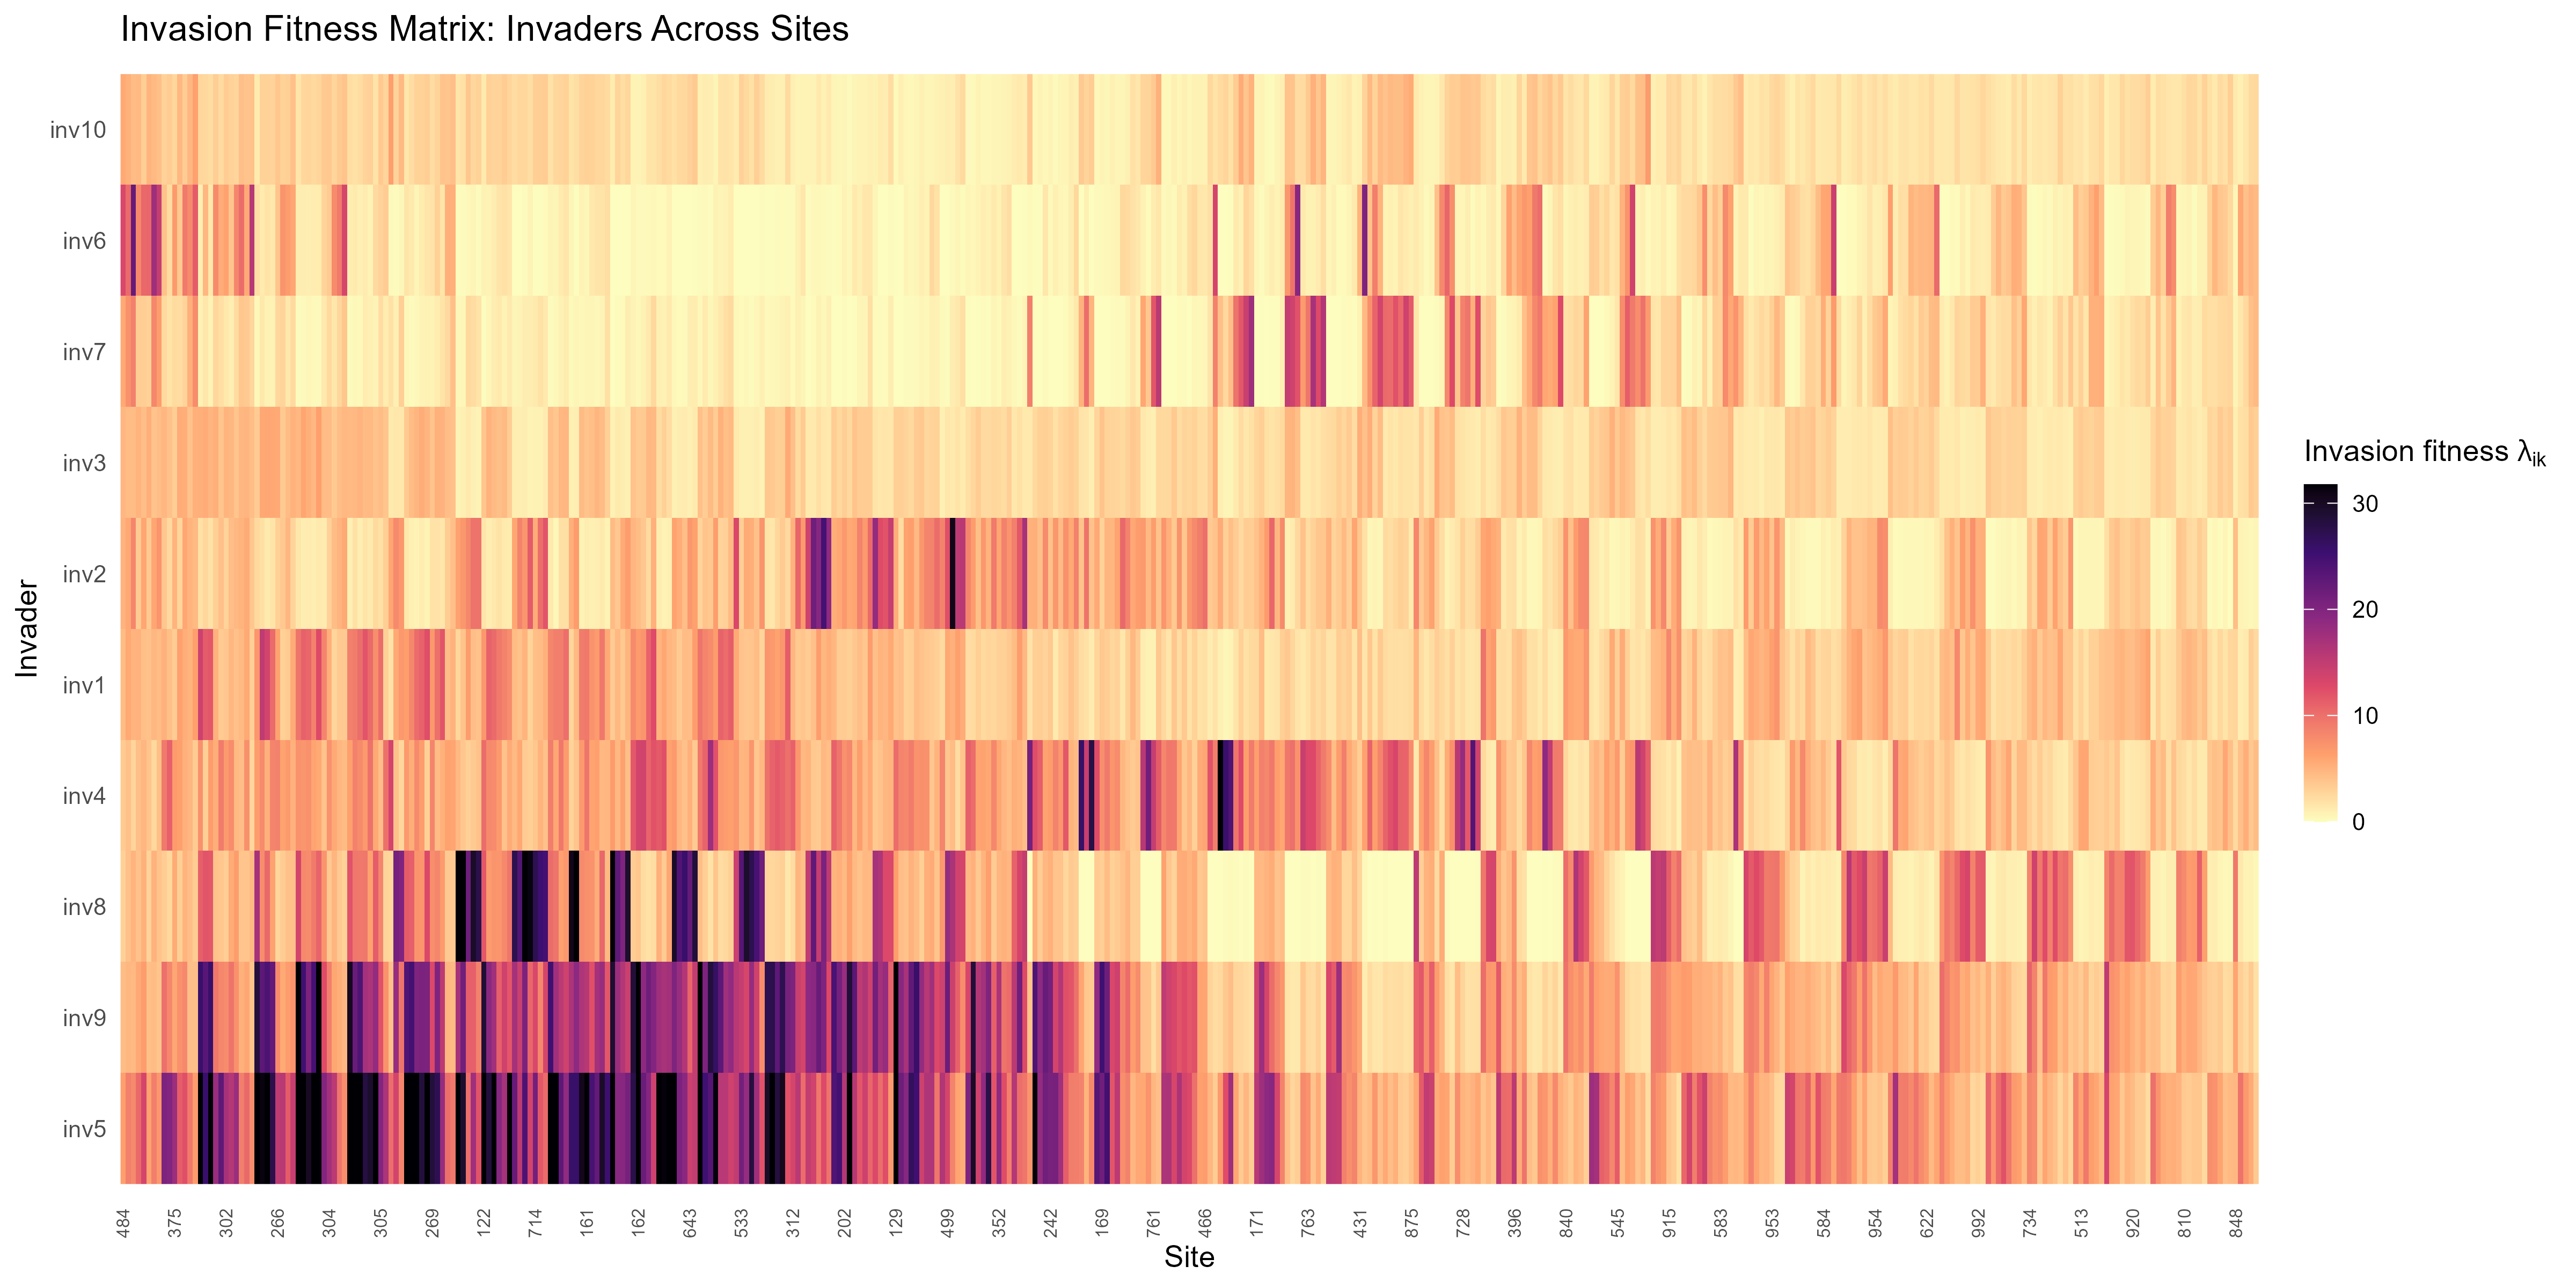
\includegraphics[width=1\linewidth]{man/figures/README-plot-fitness-1}

This figure serves as a diagnostic map of invasibility and invader
performance, feeding into later steps like risk ranking, vulnerability
hotspot mapping, or scenario testing.

\hypertarget{species-level-invasivess-i.e.-invader-ranking}{%
\subsubsection{9.2. Species-level invasivess i.e.~invader
ranking}\label{species-level-invasivess-i.e.-invader-ranking}}

We use the invasion fitness matrix to derive a \textbf{species-level
invasiveness score}, calculated as the total invasion fitness (Σ
λ\_\{i,k\}) for each invader across all sites.\\
This metric integrates biotic resistance and environmental filtering
over the full landscape, providing a single quantitative measure of
establishment potential.

Ranking invaders by this score reveals:

\begin{itemize}
\tightlist
\item
  \textbf{High-risk ``super-invaders''} --- species with high and
  geographically broad fitness, posing widespread establishment
  potential.\\
\item
  \textbf{Low-risk invaders} --- species predicted to be strongly
  excluded in most or all sites.
\end{itemize}

Such rankings are valuable for \textbf{risk prioritisation} in
management and surveillance, focusing attention on species most likely
to succeed under current community and environmental conditions.

Bar height represents cumulative invasion fitness (summed over sites).
Ordering from left to right shows highest to lowest invasiveness risk.

\begin{Shaded}
\begin{Highlighting}[]
\CommentTok{\# Sum invasion fitness across sites for each invader and order from highest to lowest}
\NormalTok{rank\_df }\OtherTok{=}\NormalTok{ lambda\_df }\SpecialCharTok{\%\textgreater{}\%}
  \FunctionTok{group\_by}\NormalTok{(invader) }\SpecialCharTok{\%\textgreater{}\%}
  \FunctionTok{summarise}\NormalTok{(}\AttributeTok{total\_lambda =} \FunctionTok{sum}\NormalTok{(lambda, }\AttributeTok{na.rm =} \ConstantTok{TRUE}\NormalTok{)) }\SpecialCharTok{\%\textgreater{}\%}
  \FunctionTok{arrange}\NormalTok{(}\FunctionTok{desc}\NormalTok{(total\_lambda)) }\SpecialCharTok{\%\textgreater{}\%}
  \FunctionTok{mutate}\NormalTok{(}\AttributeTok{invader =} \FunctionTok{factor}\NormalTok{(invader, }\AttributeTok{levels =}\NormalTok{ invader))}

\CommentTok{\# Bar plot of total invasion fitness by invader}
\FunctionTok{ggplot}\NormalTok{(rank\_df, }
       \FunctionTok{aes}\NormalTok{(}\AttributeTok{x =}\NormalTok{ invader, }\AttributeTok{y =} \FunctionTok{sqrt}\NormalTok{(total\_lambda), }\AttributeTok{fill =} \FunctionTok{sqrt}\NormalTok{(total\_lambda))) }\SpecialCharTok{+}
  \FunctionTok{geom\_col}\NormalTok{(}\AttributeTok{width =} \FloatTok{0.7}\NormalTok{, }\AttributeTok{color =} \StringTok{"grey50"}\NormalTok{) }\SpecialCharTok{+}
  \FunctionTok{scale\_fill\_viridis\_c}\NormalTok{(}\AttributeTok{option =} \StringTok{"inferno"}\NormalTok{, }
                       \AttributeTok{name =} \FunctionTok{expression}\NormalTok{(}\StringTok{"Total fitness"}\SpecialCharTok{\textasciitilde{}}\FunctionTok{sum}\NormalTok{(lambda[i]))) }\SpecialCharTok{+}
  \FunctionTok{labs}\NormalTok{(}\AttributeTok{title =} \StringTok{"Invader Ranking by Total Growth Potential"}\NormalTok{,}
       \AttributeTok{x =} \StringTok{"Invader"}\NormalTok{,}
       \AttributeTok{y =} \FunctionTok{expression}\NormalTok{(}\StringTok{"Total invasion fitness "} \SpecialCharTok{*} \FunctionTok{sum}\NormalTok{(lambda[i}\SpecialCharTok{*}\NormalTok{k]))) }\SpecialCharTok{+}
  \FunctionTok{theme\_minimal}\NormalTok{(}\AttributeTok{base\_size =} \DecValTok{12}\NormalTok{) }\SpecialCharTok{+}
  \FunctionTok{theme}\NormalTok{(}\AttributeTok{axis.text.x =} \FunctionTok{element\_text}\NormalTok{(}\AttributeTok{angle =} \DecValTok{45}\NormalTok{, }\AttributeTok{hjust =} \DecValTok{1}\NormalTok{, }\AttributeTok{vjust =} \DecValTok{1}\NormalTok{),}
        \AttributeTok{panel.grid.major.x =} \FunctionTok{element\_blank}\NormalTok{(),}
        \AttributeTok{legend.position =} \StringTok{"top"}
\NormalTok{  )}
\end{Highlighting}
\end{Shaded}

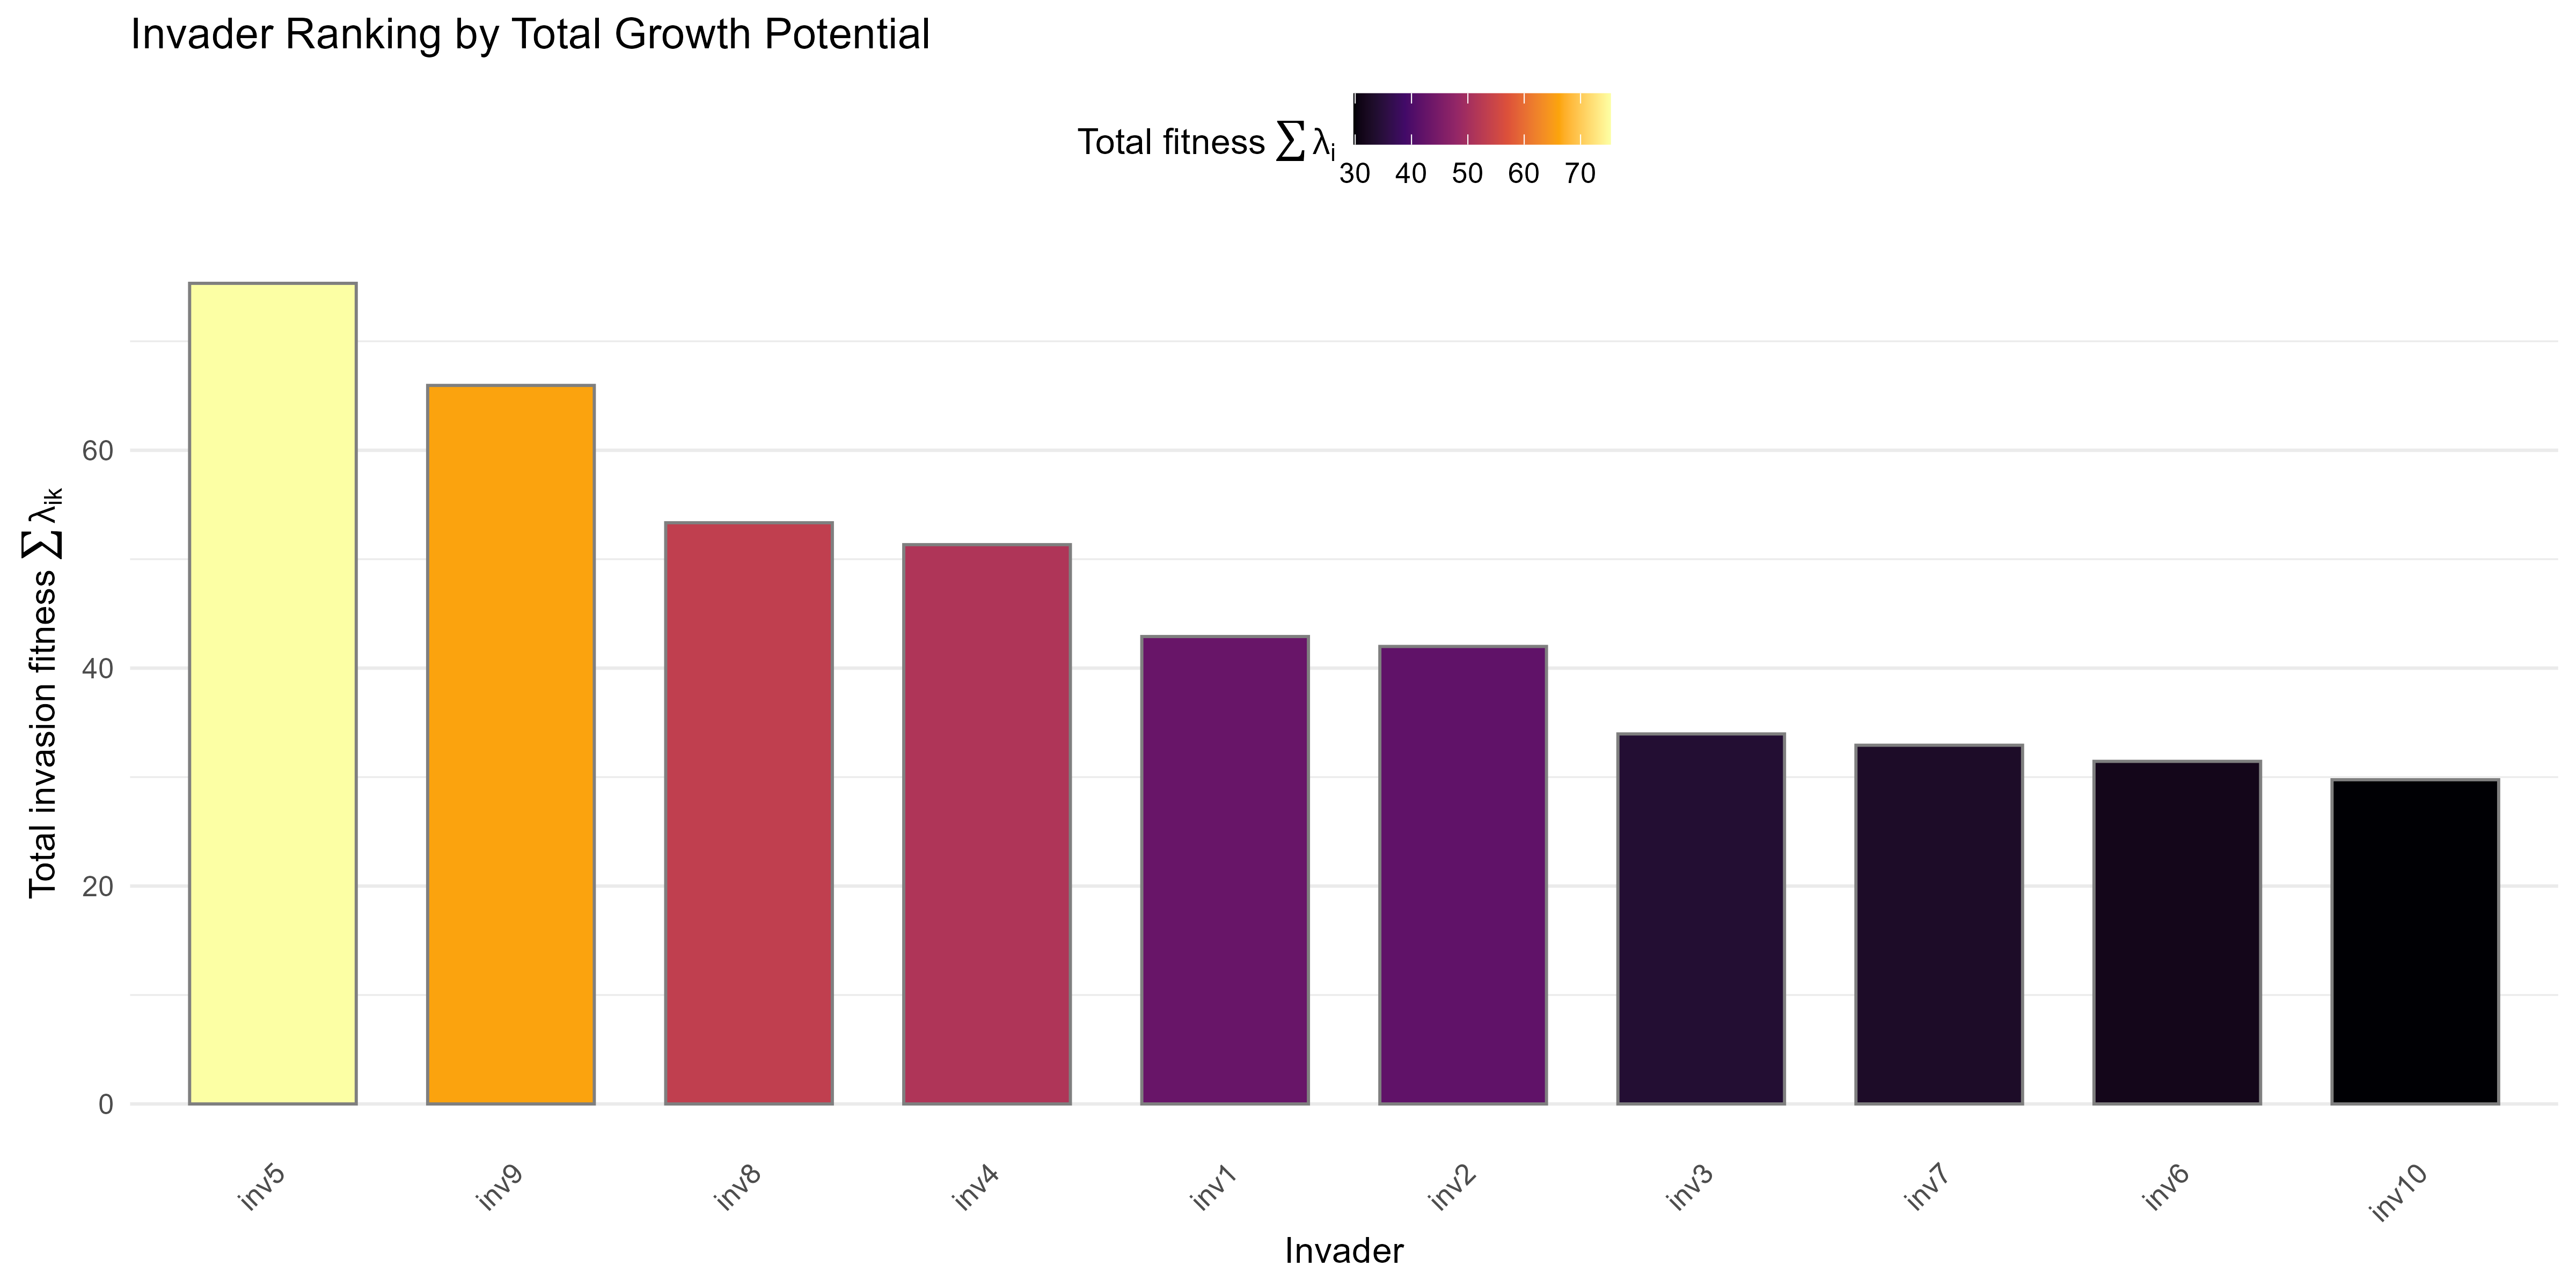
\includegraphics[width=1\linewidth]{man/figures/README-invader-rank-1}

\hypertarget{site-level-invasibility}{%
\subsubsection{9.3. Site-level
Invasibility}\label{site-level-invasibility}}

We summarise the invasion fitness matrix across invaders to quantify
\textbf{site-level invasibility} --- the openness of each community to
potential establishment.\\
For each site, we calculate:

\begin{itemize}
\tightlist
\item
  \textbf{Proportion of invaders with positive fitness}
  (\texttt{prop\_pos}) --- the fraction of simulated invaders predicted
  to establish successfully.\\
\item
  \textbf{Count of successful invaders} (\texttt{cnt\_pos}) --- number
  of invaders with λ\_\{i,k\} \textgreater{} 0.\\
\item
  \textbf{Mean invasion fitness} (\texttt{mean\_l}) --- average
  λ\_\{i,k\} across invaders, indicating general establishment
  potential.
\end{itemize}

Mapping these metrics spatially reveals:

\begin{itemize}
\tightlist
\item
  \textbf{Hotspots} --- sites with high \texttt{prop\_pos}, indicating
  low biotic resistance and/or favourable abiotic conditions.\\
\item
  \textbf{Potential refugia} --- sites with low \texttt{prop\_pos},
  where community structure or environmental conditions limit
  establishment.
\end{itemize}

Labels inside tiles show \texttt{cnt\_pos}, aiding interpretation of
proportional risk in terms of absolute invader counts.

\begin{Shaded}
\begin{Highlighting}[]
\CommentTok{\# Summarize invasion fitness at each site:}
\NormalTok{site\_sum }\OtherTok{=}\NormalTok{ lambda\_df }\SpecialCharTok{\%\textgreater{}\%}
  \FunctionTok{group\_by}\NormalTok{(site\_id, x, y) }\SpecialCharTok{\%\textgreater{}\%}
  \FunctionTok{summarize}\NormalTok{(}
    \AttributeTok{mean\_l   =} \FunctionTok{mean}\NormalTok{(lambda),             }\CommentTok{\# Mean invasion fitness across invaders}
    \AttributeTok{prop\_pos =} \FunctionTok{mean}\NormalTok{(lambda }\SpecialCharTok{\textgreater{}} \DecValTok{0}\NormalTok{),         }\CommentTok{\# Proportion of invaders with positive fitness}
    \AttributeTok{cnt\_pos  =} \FunctionTok{sum}\NormalTok{(lambda }\SpecialCharTok{\textgreater{}} \DecValTok{0}\NormalTok{),          }\CommentTok{\# Number of successful invaders}
    \AttributeTok{cnt\_neg  =} \FunctionTok{sum}\NormalTok{(lambda }\SpecialCharTok{\textless{}} \DecValTok{0}\NormalTok{)           }\CommentTok{\# Number of unsuccessful invaders}
\NormalTok{  ) }\SpecialCharTok{\%\textgreater{}\%}
  \FunctionTok{ungroup}\NormalTok{()}

\CommentTok{\# Map proportion of successful invaders at each site}
\FunctionTok{ggplot}\NormalTok{(site\_sum, }\FunctionTok{aes}\NormalTok{(}\AttributeTok{x =}\NormalTok{ x, }\AttributeTok{y =}\NormalTok{ y, }\AttributeTok{fill =}\NormalTok{ prop\_pos)) }\SpecialCharTok{+}
  \FunctionTok{geom\_tile}\NormalTok{(}\AttributeTok{color =} \ConstantTok{NA}\NormalTok{) }\SpecialCharTok{+}
  \FunctionTok{geom\_sf}\NormalTok{(}\AttributeTok{data =}\NormalTok{ rsa, }\AttributeTok{inherit.aes =} \ConstantTok{FALSE}\NormalTok{, }\AttributeTok{fill =} \ConstantTok{NA}\NormalTok{, }\AttributeTok{color =} \StringTok{"black"}\NormalTok{, }\AttributeTok{size =} \FloatTok{0.5}\NormalTok{) }\SpecialCharTok{+}
  \FunctionTok{scale\_fill\_viridis\_c}\NormalTok{(}\AttributeTok{option =} \StringTok{"rocket"}\NormalTok{, }
                       \AttributeTok{labels =}\NormalTok{ scales}\SpecialCharTok{::}\FunctionTok{percent\_format}\NormalTok{(}\AttributeTok{accuracy =} \DecValTok{1}\NormalTok{),}
                       \AttributeTok{name =} \StringTok{"\% Invaders with}\SpecialCharTok{\textbackslash{}n}\StringTok{Positive Fitness"}\NormalTok{) }\SpecialCharTok{+}
  \FunctionTok{geom\_text}\NormalTok{(}\FunctionTok{aes}\NormalTok{(}\AttributeTok{label =}\NormalTok{ cnt\_pos), }\AttributeTok{color =} \StringTok{"white"}\NormalTok{, }\AttributeTok{size =} \FloatTok{2.5}\NormalTok{) }\SpecialCharTok{+} 
  \FunctionTok{coord\_sf}\NormalTok{() }\SpecialCharTok{+}
  \FunctionTok{labs}\NormalTok{(}\AttributeTok{title =} \StringTok{"Site{-}level Invasibility (Proportion of Successful Invaders)"}\NormalTok{, }
       \AttributeTok{x =} \StringTok{"Longitude"}\NormalTok{, }\AttributeTok{y =} \StringTok{"Latitude"}\NormalTok{) }\SpecialCharTok{+}
  \FunctionTok{theme\_minimal}\NormalTok{(}\AttributeTok{base\_size =} \DecValTok{12}\NormalTok{) }\SpecialCharTok{+}
  \FunctionTok{theme}\NormalTok{(}\AttributeTok{panel.grid =} \FunctionTok{element\_blank}\NormalTok{())}
\end{Highlighting}
\end{Shaded}

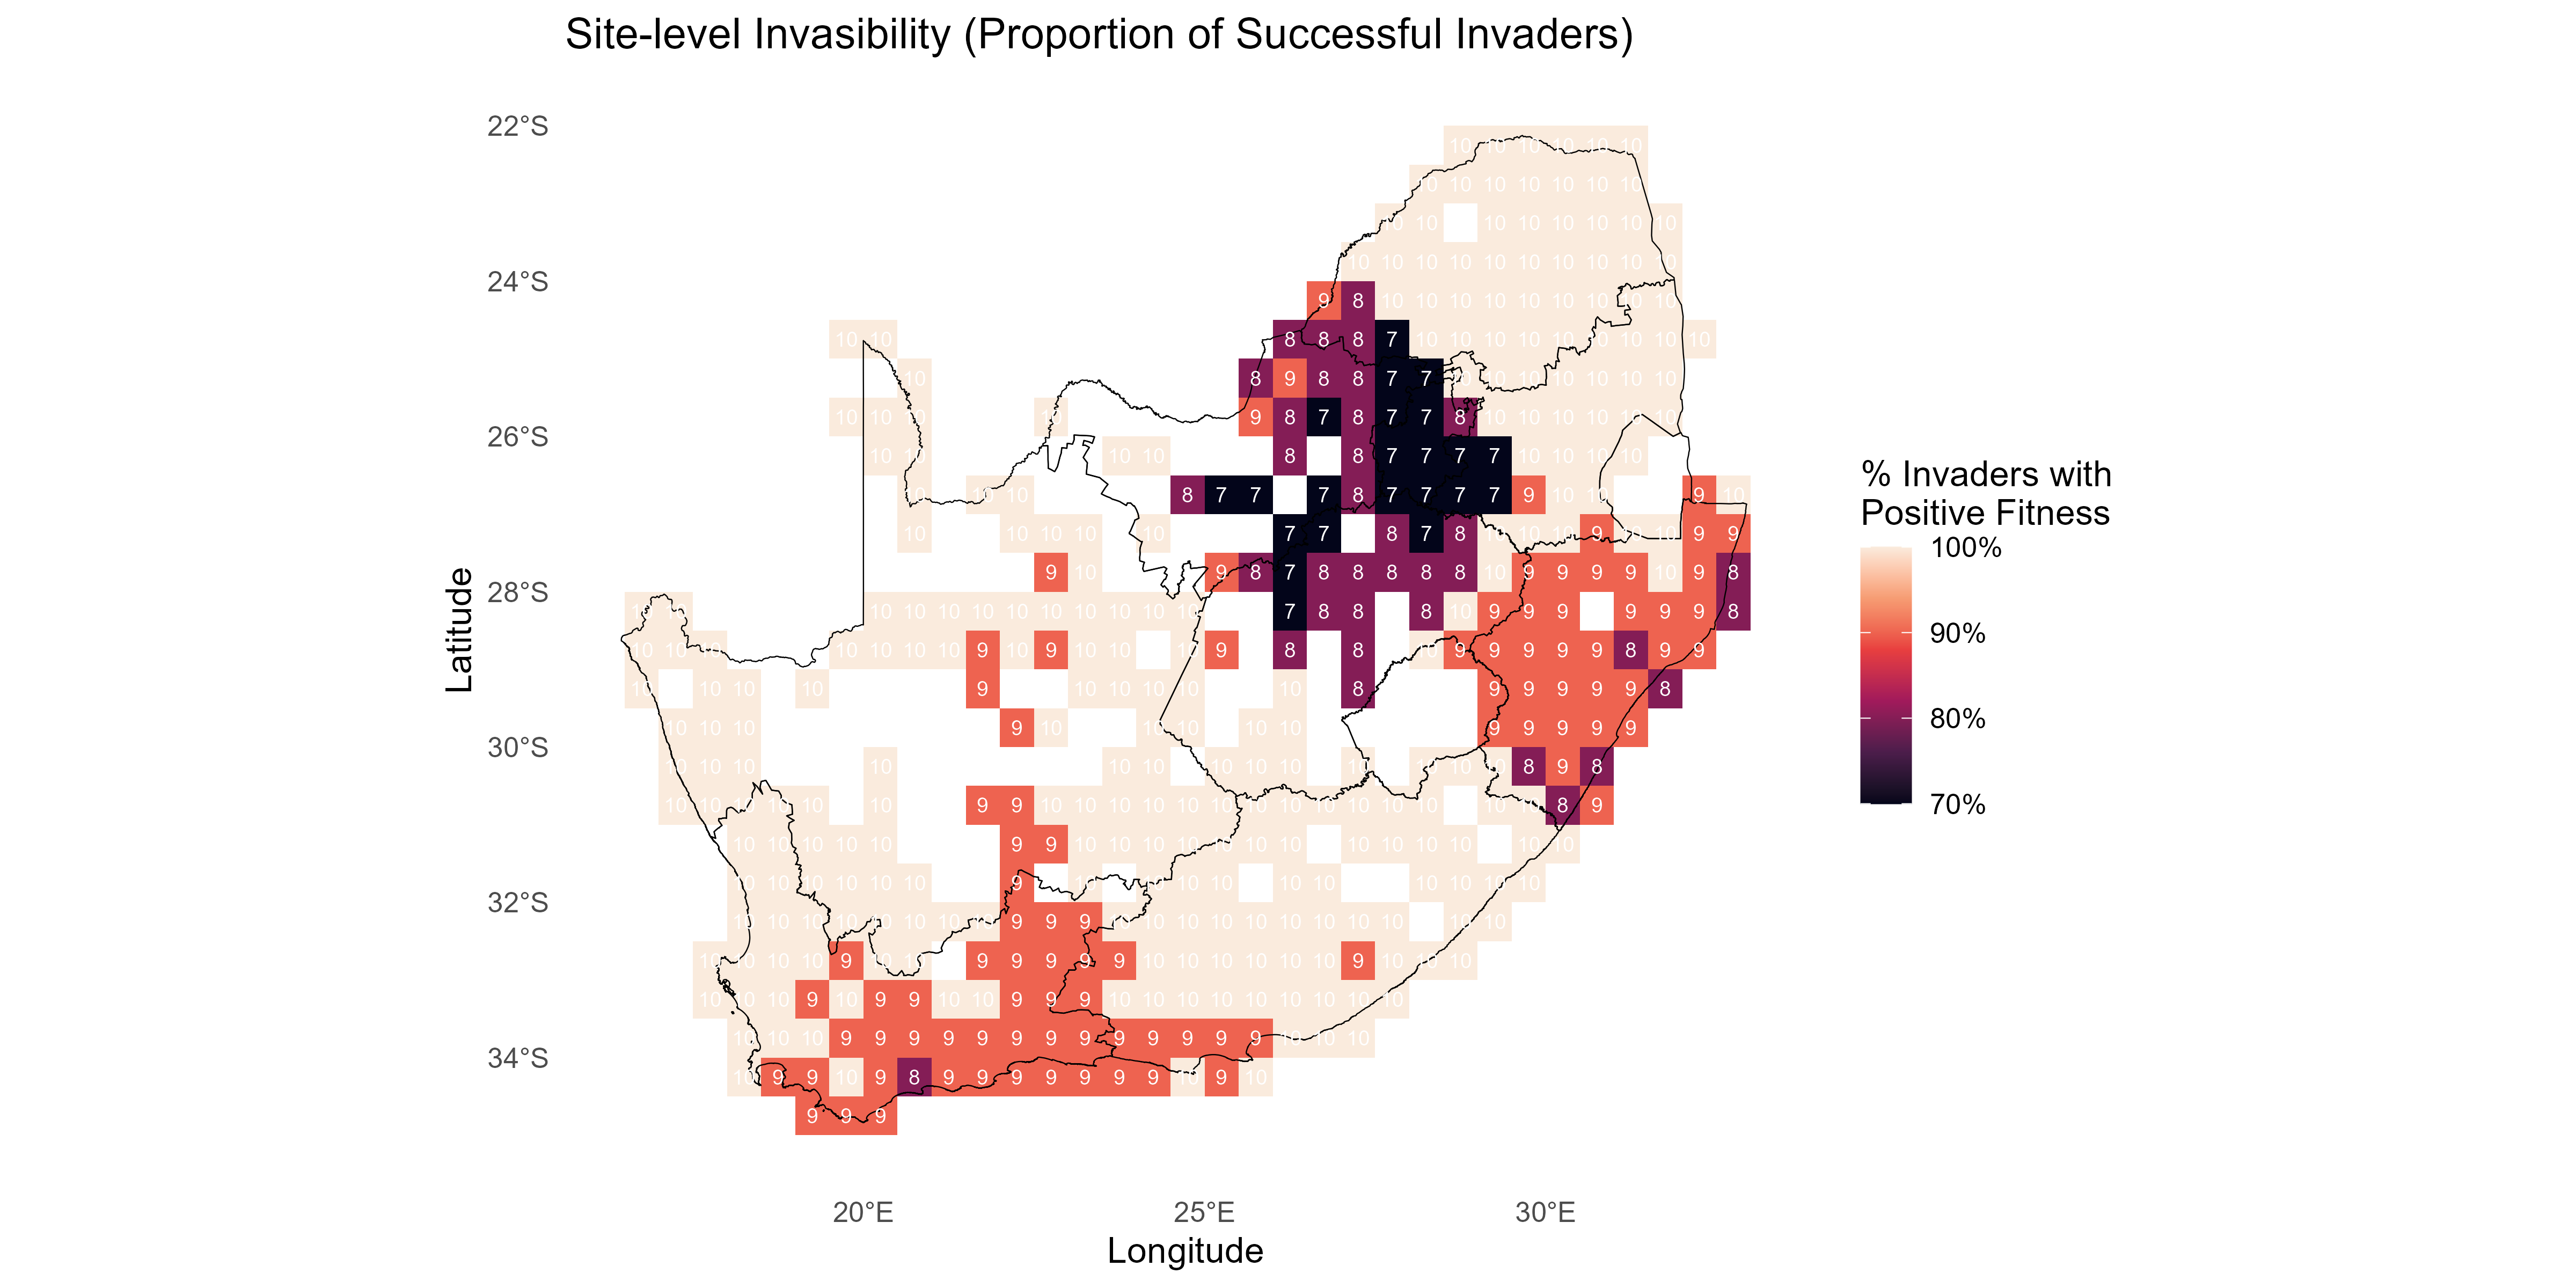
\includegraphics[width=1\linewidth]{man/figures/README-site-invasibility-1}

\hypertarget{mean-species-invasivess-by-site}{%
\subsubsection{9.4. Mean species invasivess by
Site}\label{mean-species-invasivess-by-site}}

We map the \textbf{mean invasion fitness} of all simulated invaders at
each site to produce a continuous measure of \textbf{community
openness}.\\
This index reflects the \emph{average} predicted establishment potential
across invaders:

\begin{itemize}
\tightlist
\item
  \textbf{High mean values} --- communities that, on average, offer
  favourable conditions and/or low competitive resistance to a broad
  range of potential invaders.\\
\item
  \textbf{Low mean values} --- communities that are generally resistant
  to establishment, either due to environmental mismatch, strong
  resident competition, or both.
\end{itemize}

This metric complements the proportion-based invasibility map (Section
9.3) by highlighting \emph{magnitude} of fitness rather than just binary
success. Sites with moderately high mean values but low proportions may
be susceptible to a few highly adapted invaders --- a pattern worth
monitoring.

\begin{Shaded}
\begin{Highlighting}[]
\CommentTok{\# Map the mean invasion fitness of all invaders at each site}
\FunctionTok{ggplot}\NormalTok{(site\_sum, }\FunctionTok{aes}\NormalTok{(}\AttributeTok{x =}\NormalTok{ x, }\AttributeTok{y =}\NormalTok{ y, }\AttributeTok{fill =}\NormalTok{ mean\_l)) }\SpecialCharTok{+}
  \FunctionTok{geom\_tile}\NormalTok{(}\AttributeTok{color =} \ConstantTok{NA}\NormalTok{) }\SpecialCharTok{+}
  \FunctionTok{geom\_sf}\NormalTok{(}\AttributeTok{data =}\NormalTok{ rsa, }\AttributeTok{inherit.aes =} \ConstantTok{FALSE}\NormalTok{, }\AttributeTok{fill =} \ConstantTok{NA}\NormalTok{, }\AttributeTok{color =} \StringTok{"black"}\NormalTok{, }\AttributeTok{size =} \FloatTok{0.5}\NormalTok{) }\SpecialCharTok{+}
  \FunctionTok{scale\_fill\_viridis\_c}\NormalTok{(}\AttributeTok{option =} \StringTok{"turbo"}\NormalTok{, }\AttributeTok{name =} \StringTok{"Mean invasion}\SpecialCharTok{\textbackslash{}n}\StringTok{fitness"}\NormalTok{) }\SpecialCharTok{+}
  \CommentTok{\# Optional: annotate with number of successful invaders}
  \CommentTok{\# geom\_text(aes(label = cnt\_pos), color = "white", size = 1.5) +}
  \FunctionTok{coord\_sf}\NormalTok{() }\SpecialCharTok{+}
  \FunctionTok{labs}\NormalTok{(}\AttributeTok{title =} \StringTok{"Mean Species Invasivess by Site (All Invaders)"}\NormalTok{, }
       \AttributeTok{x =} \StringTok{"Longitude"}\NormalTok{,}
       \AttributeTok{y =} \StringTok{"Latitude"}\NormalTok{) }\SpecialCharTok{+}
  \FunctionTok{theme\_minimal}\NormalTok{(}\AttributeTok{base\_size =} \DecValTok{12}\NormalTok{) }\SpecialCharTok{+}
  \FunctionTok{theme}\NormalTok{(}\AttributeTok{panel.grid =} \FunctionTok{element\_blank}\NormalTok{())}
\end{Highlighting}
\end{Shaded}

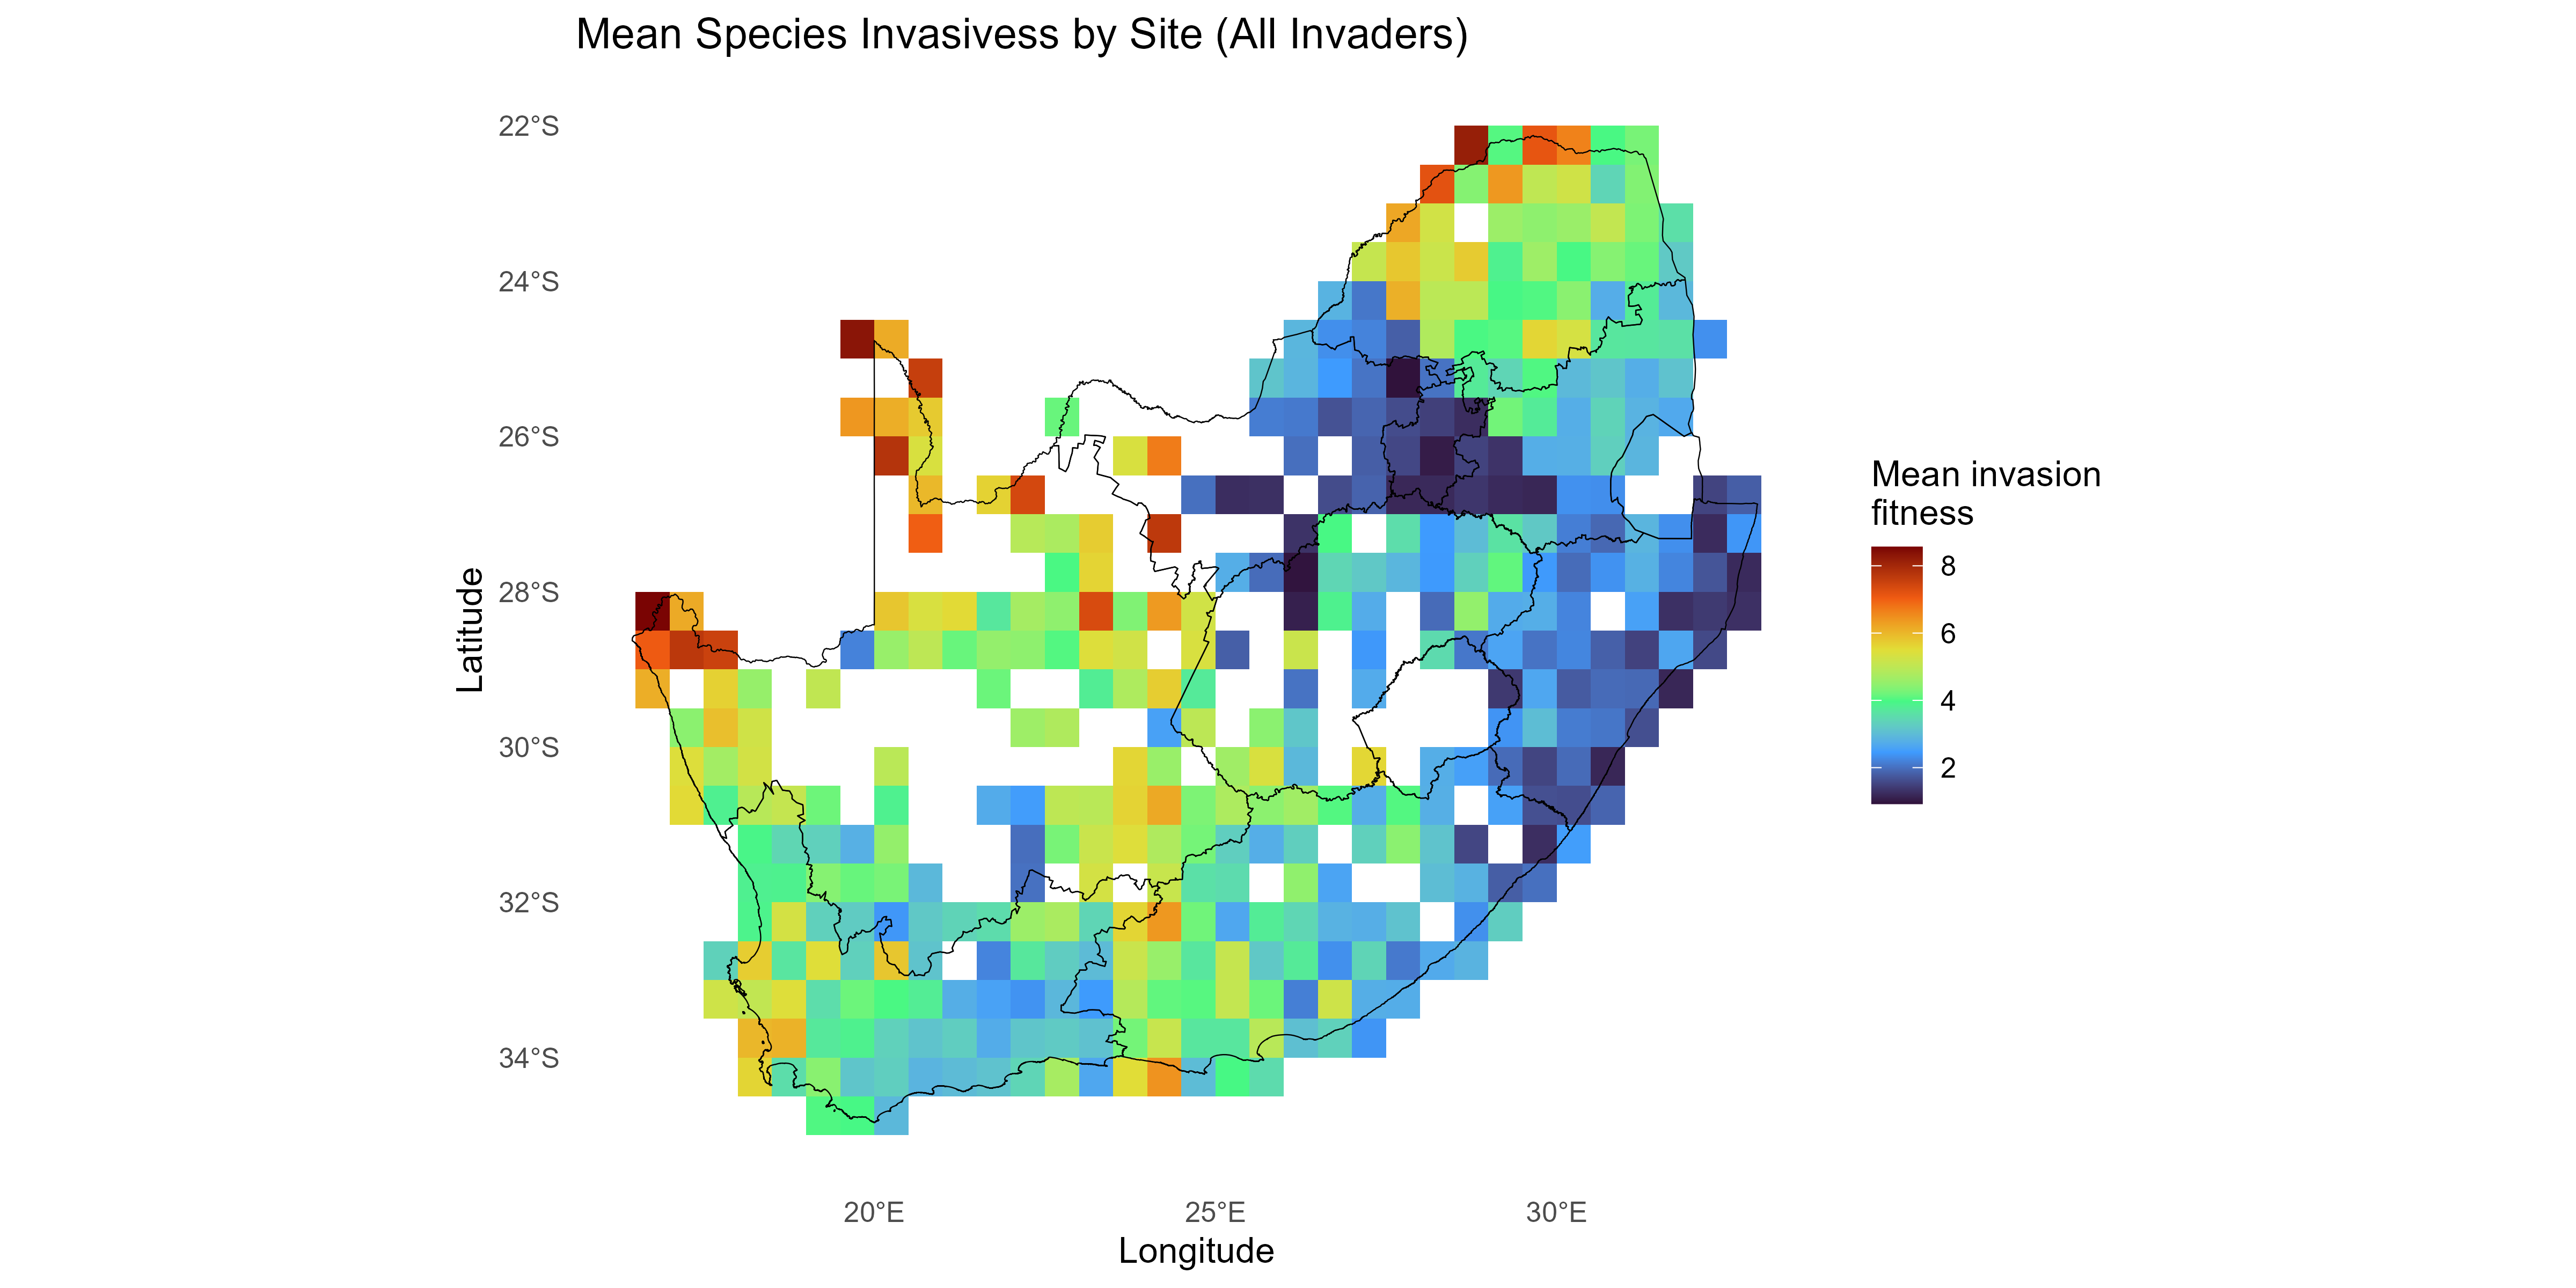
\includegraphics[width=1\linewidth]{man/figures/README-spp-invasiness-1}

\begin{center}\rule{0.5\linewidth}{0.5pt}\end{center}

\hypertarget{clusters-of-invasibility-and-invasiness}{%
\subsection{10. Clusters of Invasibility and
Invasiness}\label{clusters-of-invasibility-and-invasiness}}

This section identifies \textbf{groups (``clusters'') of sites and
invaders} that share similar patterns of invasion risk and opportunity,
based on hierarchical clustering of the invasion fitness matrix. These
analyses enable detection of ecological syndromes i.e., types of sites
most at risk, or types of invaders most threatening, facilitating
targeted monitoring and management.

\hypertarget{hierarchical-clustering-of-invasion-fitness}{%
\subsubsection{10.1. Hierarchical clustering of invasion
fitness}\label{hierarchical-clustering-of-invasion-fitness}}

We use hierarchical clustering to group both sites and invaders
according to their invasion fitness profiles, i.e., the patterns of
predicted establishment success across the landscape. The heatmap
visually summarizes these relationships:

\begin{itemize}
\tightlist
\item
  \textbf{Rows} = invaders, \textbf{columns} = sites\\
\item
  \textbf{Cells} = invasion fitness (\(\lambda_{i,k}\))\\
\item
  \textbf{Dendrograms} = hierarchical clusters (similarity in invasion
  profile)
\end{itemize}

This highlights both ``types'' of invaders (e.g., those that succeed
broadly, or only in a few sites) and ``types'' of sites (e.g., open to
many invaders vs.~resistant). Clustering also underpins categorical risk
labeling in subsequent sections.

\begin{Shaded}
\begin{Highlighting}[]
\FunctionTok{library}\NormalTok{(pheatmap)}

\CommentTok{\# Remove invaders (rows) and sites (columns) with all NA values (if present)}
\CommentTok{\# This ensures only meaningful data are visualized and clustered}
\NormalTok{lambda\_mat\_noNA }\OtherTok{=}\NormalTok{ lambda\_mat[}\FunctionTok{rowSums}\NormalTok{(}\FunctionTok{is.na}\NormalTok{(lambda\_mat)) }\SpecialCharTok{\textless{}} \FunctionTok{ncol}\NormalTok{(lambda\_mat),}
                             \FunctionTok{colSums}\NormalTok{(}\FunctionTok{is.na}\NormalTok{(lambda\_mat)) }\SpecialCharTok{\textless{}} \FunctionTok{nrow}\NormalTok{(lambda\_mat)]}

\CommentTok{\# Clustered heatmap of invasion fitness matrix (invader × site)}
\CommentTok{\# {-} Each cell shows the invasion fitness (lambda) for a given invader{-}site pair}
\CommentTok{\# {-} Hierarchical clustering groups similar invaders and similar sites}
\FunctionTok{pheatmap}\NormalTok{(lambda\_mat\_noNA,}
         \AttributeTok{color =} \FunctionTok{rev}\NormalTok{(viridis}\SpecialCharTok{::}\FunctionTok{viridis}\NormalTok{(}\DecValTok{100}\NormalTok{, }\AttributeTok{option =} \StringTok{"viridis"}\NormalTok{)),}
         \AttributeTok{clustering\_distance\_rows =} \StringTok{"euclidean"}\NormalTok{,}
         \AttributeTok{clustering\_distance\_cols =} \StringTok{"euclidean"}\NormalTok{,}
         \AttributeTok{clustering\_method =} \StringTok{"complete"}\NormalTok{,}
         \AttributeTok{fontsize\_row =} \DecValTok{8}\NormalTok{, }\AttributeTok{fontsize\_col =} \DecValTok{8}\NormalTok{,}
         \AttributeTok{main =} \StringTok{"Clustered Invasion Fitness Matrix (Invader × Site)"}\NormalTok{,}
         \AttributeTok{angle\_col =} \DecValTok{45}\NormalTok{)}
\end{Highlighting}
\end{Shaded}

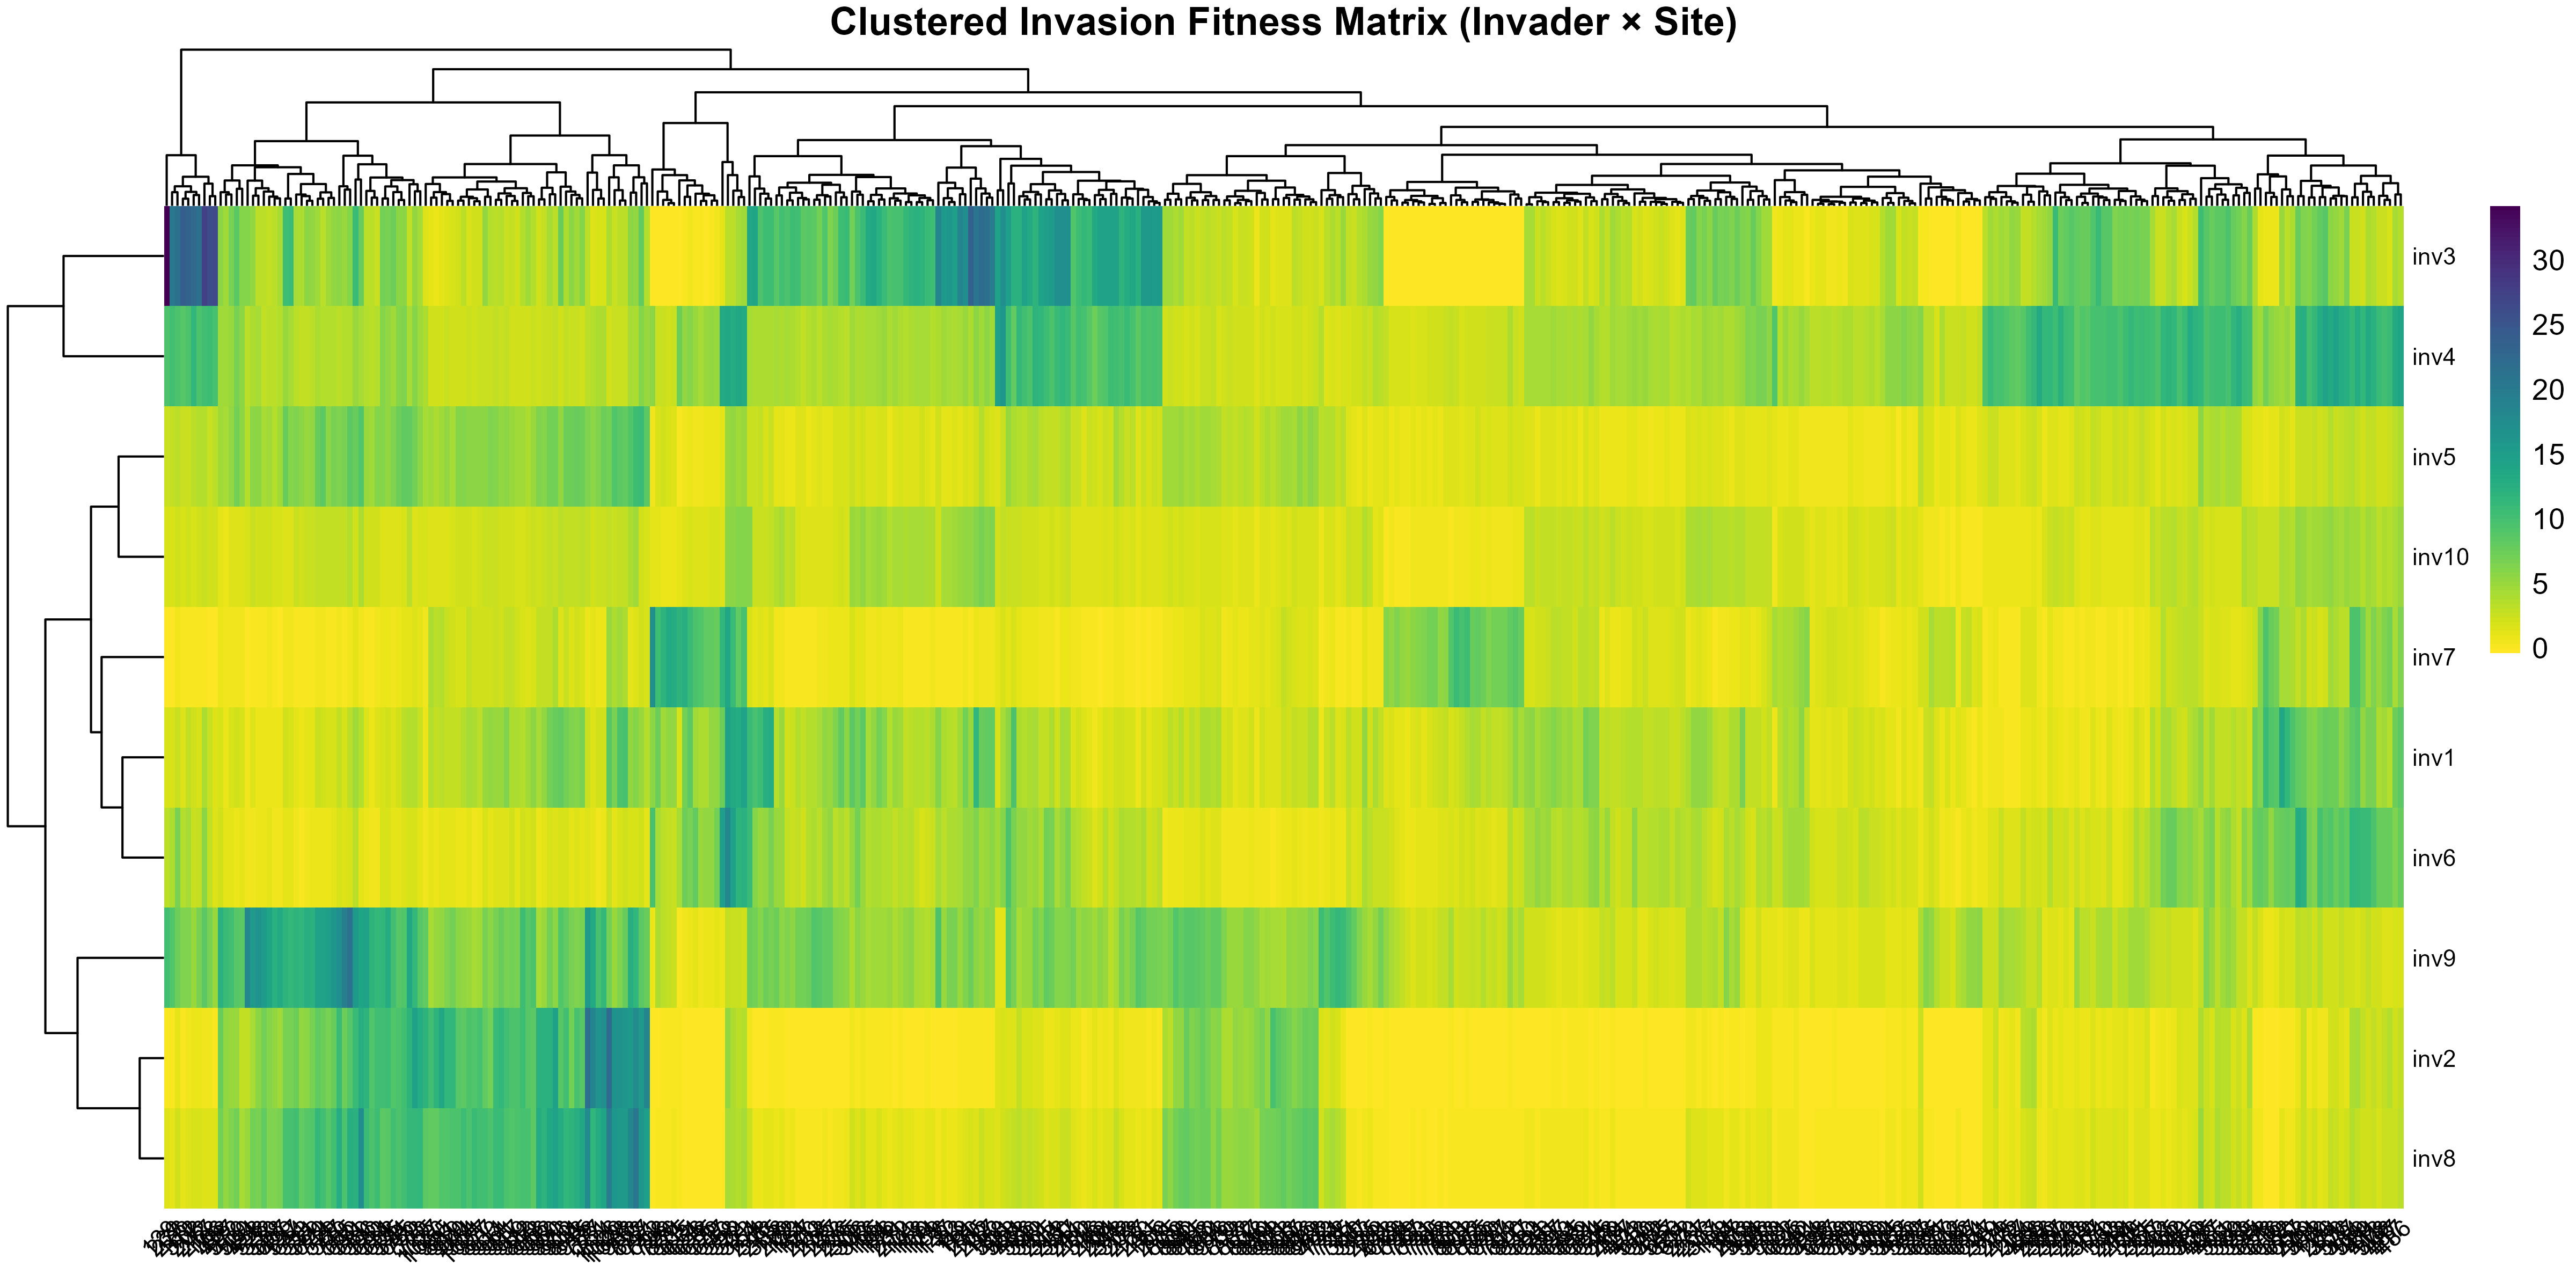
\includegraphics[width=1\linewidth]{man/figures/README-fitness-cluster-1}

\begin{Shaded}
\begin{Highlighting}[]

\CommentTok{\# Assign invaders and sites to discrete clusters (syndromes) for downstream visualization}
\CommentTok{\# Sites: cluster by invasion fitness profile (columns)}
\NormalTok{site\_dist }\OtherTok{=} \FunctionTok{dist}\NormalTok{(}\FunctionTok{t}\NormalTok{(lambda\_mat\_noNA))                    }\CommentTok{\# Compute pairwise distances between sites}
\NormalTok{site\_clust }\OtherTok{=} \FunctionTok{hclust}\NormalTok{(site\_dist, }\AttributeTok{method =} \StringTok{"ward.D2"}\NormalTok{)      }\CommentTok{\# Hierarchical clustering}
\NormalTok{site\_groups }\OtherTok{=} \FunctionTok{cutree}\NormalTok{(site\_clust, }\AttributeTok{k =} \DecValTok{5}\NormalTok{)                 }\CommentTok{\# Assign each site to one of 5 clusters}

\CommentTok{\# Invaders: cluster by fitness profile across sites (rows)}
\NormalTok{invader\_dist }\OtherTok{=} \FunctionTok{dist}\NormalTok{(lambda\_mat\_noNA)                    }\CommentTok{\# Compute pairwise distances between invaders}
\NormalTok{invader\_clust }\OtherTok{=} \FunctionTok{hclust}\NormalTok{(invader\_dist, }\AttributeTok{method =} \StringTok{"ward.D2"}\NormalTok{)}
\NormalTok{invader\_groups }\OtherTok{=} \FunctionTok{cutree}\NormalTok{(invader\_clust, }\AttributeTok{k =} \DecValTok{5}\NormalTok{)           }\CommentTok{\# Assign each invader to one of 5 clusters}

\CommentTok{\# Attach cluster labels to site and invader summary dataframes}
\CommentTok{\# Add site cluster group to site summary dataframe (site\_sum)}
\CommentTok{\# site\_id must match the column names of lambda\_mat\_noNA}
\NormalTok{site\_sum}\SpecialCharTok{$}\NormalTok{site\_cluster }\OtherTok{=} \FunctionTok{factor}\NormalTok{(site\_groups[site\_sum}\SpecialCharTok{$}\NormalTok{site\_id])}

\CommentTok{\# Add invader cluster group to long{-}form fitness dataframe (lambda\_df)}
\CommentTok{\# invader must match the row names of lambda\_mat\_noNA}
\NormalTok{lambda\_df}\SpecialCharTok{$}\NormalTok{invader\_cluster }\OtherTok{=} \FunctionTok{factor}\NormalTok{(invader\_groups[lambda\_df}\SpecialCharTok{$}\NormalTok{invader])}

\CommentTok{\# These cluster assignments can be used for:}
\CommentTok{\# {-} Color{-}coding sites and invaders in subsequent plots}
\CommentTok{\# {-} Group{-}based analyses or statistical comparisons}
\CommentTok{\# {-} Mapping spatial patterns of invasion risk by ecological “syndrome”}
\end{Highlighting}
\end{Shaded}

\hypertarget{map-site-invasion-risk}{%
\subsubsection{10.2. Map Site Invasion
Risk}\label{map-site-invasion-risk}}

We next summarize and map site-level risk based on cluster assignments,
providing a spatial overview of invasibility ``syndromes'':

\begin{itemize}
\tightlist
\item
  \textbf{High-risk categories} indicate site clusters that are
  generally open to invasion by a broad range of invaders.
\item
  \textbf{Low-risk categories} correspond to more robust,
  invasion-resistant communities.
\end{itemize}

Descriptive category labels (``very-high'' to ``very-low'') provide an
interpretable mapping of site clusters to ecological risk.

\begin{Shaded}
\begin{Highlighting}[]
\CommentTok{\# Summarize mean invasion fitness for each invader, grouped by their cluster assignment}
\NormalTok{invader\_summary }\OtherTok{=}\NormalTok{ lambda\_df }\SpecialCharTok{\%\textgreater{}\%}
  \FunctionTok{group\_by}\NormalTok{(invader, invader\_cluster) }\SpecialCharTok{\%\textgreater{}\%}
  \FunctionTok{summarise}\NormalTok{(}\AttributeTok{mean\_lambda =} \FunctionTok{mean}\NormalTok{(lambda, }\AttributeTok{na.rm =} \ConstantTok{TRUE}\NormalTok{), }\AttributeTok{.groups =} \StringTok{"drop"}\NormalTok{)}

\CommentTok{\# Compute overall mean invasion fitness for each invader cluster (highest to lowest)}
\NormalTok{cluster\_means }\OtherTok{=}\NormalTok{ invader\_summary }\SpecialCharTok{\%\textgreater{}\%}
  \FunctionTok{group\_by}\NormalTok{(invader\_cluster) }\SpecialCharTok{\%\textgreater{}\%}
  \FunctionTok{summarise}\NormalTok{(}\AttributeTok{cluster\_mean =} \FunctionTok{mean}\NormalTok{(mean\_lambda, }\AttributeTok{na.rm =} \ConstantTok{TRUE}\NormalTok{)) }\SpecialCharTok{\%\textgreater{}\%}
  \FunctionTok{arrange}\NormalTok{(}\FunctionTok{desc}\NormalTok{(cluster\_mean))  }\CommentTok{\# Order clusters from highest to lowest mean fitness}

\CommentTok{\# Define category labels in descending order of risk/friendly invasion fitness}
\NormalTok{category\_labels }\OtherTok{=} \FunctionTok{c}\NormalTok{(}\StringTok{"very{-}high"}\NormalTok{, }\StringTok{"high"}\NormalTok{, }\StringTok{"medium"}\NormalTok{, }\StringTok{"low"}\NormalTok{, }\StringTok{"very{-}low"}\NormalTok{)[}\DecValTok{1}\SpecialCharTok{:}\FunctionTok{nrow}\NormalTok{(cluster\_means)]}

\CommentTok{\# Create a named vector to recode numeric cluster assignments to descriptive categories}
\NormalTok{cluster\_map }\OtherTok{=} \FunctionTok{setNames}\NormalTok{(category\_labels, cluster\_means}\SpecialCharTok{$}\NormalTok{invader\_cluster)}

\CommentTok{\# Map invader clusters to descriptive categories, preserving order for plotting}
\NormalTok{invader\_summary }\OtherTok{=}\NormalTok{ invader\_summary }\SpecialCharTok{\%\textgreater{}\%}
  \FunctionTok{mutate}\NormalTok{(}\AttributeTok{invader\_category =} \FunctionTok{factor}\NormalTok{(cluster\_map[}\FunctionTok{as.character}\NormalTok{(invader\_cluster)],}
                                   \AttributeTok{levels =}\NormalTok{ category\_labels))}

\CommentTok{\# Assign each invader to a descriptive invasion risk category based on its cluster,}
\CommentTok{\# ensuring categories are ordered for consistent plotting and analysis}
\NormalTok{lambda\_df }\OtherTok{=}\NormalTok{ lambda\_df }\SpecialCharTok{\%\textgreater{}\%}
  \FunctionTok{mutate}\NormalTok{(}\AttributeTok{invader\_category =} \FunctionTok{factor}\NormalTok{(cluster\_map[}\FunctionTok{as.character}\NormalTok{(invader\_cluster)],}
                                   \AttributeTok{levels =}\NormalTok{ category\_labels))}

\CommentTok{\# (Optional) Plot: Distribution of mean invasion fitness by descriptive invader category}
\CommentTok{\# ggplot(invader\_summary, aes(x = invader\_category, y = mean\_lambda, fill = invader\_category)) +}
\CommentTok{\#   geom\_boxplot() +}
\CommentTok{\#   scale\_fill\_brewer(palette = "RdYlBu", direction = 1, guide = "none") +}
\CommentTok{\#   labs(}
\CommentTok{\#     title = "Mean Invasion Fitness by Invader Category",}
\CommentTok{\#     x = "Invader Category",}
\CommentTok{\#     y = "Mean Invasion Fitness"}
\CommentTok{\#   ) +}
\CommentTok{\#   theme\_minimal(base\_size = 12)}


\CommentTok{\# Repeat for site clusters: mean invasion fitness for each site cluster}
\CommentTok{\# Calculate mean invasion fitness for each site cluster and order}
\NormalTok{site\_category\_df }\OtherTok{=}\NormalTok{ site\_sum }\SpecialCharTok{\%\textgreater{}\%}
  \FunctionTok{group\_by}\NormalTok{(site\_cluster) }\SpecialCharTok{\%\textgreater{}\%}
  \FunctionTok{summarise}\NormalTok{(}\AttributeTok{mean\_fitness =} \FunctionTok{mean}\NormalTok{(mean\_l, }\AttributeTok{na.rm =} \ConstantTok{TRUE}\NormalTok{)) }\SpecialCharTok{\%\textgreater{}\%}
  \FunctionTok{arrange}\NormalTok{(}\FunctionTok{desc}\NormalTok{(mean\_fitness))}

\CommentTok{\# Assign descriptive category labels to site clusters}
\NormalTok{site\_labels }\OtherTok{=} \FunctionTok{c}\NormalTok{(}\StringTok{"very{-}high"}\NormalTok{, }\StringTok{"high"}\NormalTok{, }\StringTok{"medium"}\NormalTok{, }\StringTok{"low"}\NormalTok{, }\StringTok{"very{-}low"}\NormalTok{)[}\DecValTok{1}\SpecialCharTok{:}\FunctionTok{nrow}\NormalTok{(site\_category\_df)]}
\NormalTok{site\_map }\OtherTok{=} \FunctionTok{setNames}\NormalTok{(site\_labels, site\_category\_df}\SpecialCharTok{$}\NormalTok{site\_cluster)}

\NormalTok{site\_sum }\OtherTok{=}\NormalTok{ site\_sum }\SpecialCharTok{\%\textgreater{}\%}
  \FunctionTok{mutate}\NormalTok{(}\AttributeTok{site\_category =} \FunctionTok{factor}\NormalTok{(site\_map[}\FunctionTok{as.character}\NormalTok{(site\_cluster)], }\AttributeTok{levels =}\NormalTok{ site\_labels))}

\CommentTok{\# Map: spatial pattern of site risk categories}
\FunctionTok{ggplot}\NormalTok{(site\_sum, }\FunctionTok{aes}\NormalTok{(}\AttributeTok{x =}\NormalTok{ x, }\AttributeTok{y =}\NormalTok{ y, }\AttributeTok{fill =}\NormalTok{ site\_category)) }\SpecialCharTok{+}
  \FunctionTok{geom\_tile}\NormalTok{(}\AttributeTok{color =} \ConstantTok{NA}\NormalTok{) }\SpecialCharTok{+}
  \FunctionTok{geom\_sf}\NormalTok{(}\AttributeTok{data =}\NormalTok{ rsa, }\AttributeTok{inherit.aes =} \ConstantTok{FALSE}\NormalTok{, }\AttributeTok{fill =} \ConstantTok{NA}\NormalTok{, }\AttributeTok{color =} \StringTok{"black"}\NormalTok{, }\AttributeTok{size =} \FloatTok{0.5}\NormalTok{) }\SpecialCharTok{+}
  \FunctionTok{scale\_fill\_brewer}\NormalTok{(}
    \AttributeTok{palette =} \StringTok{"RdYlBu"}\NormalTok{,}
    \AttributeTok{direction =} \DecValTok{1}\NormalTok{,}
    \AttributeTok{name =} \StringTok{"Site Invasibility"}
\NormalTok{  ) }\SpecialCharTok{+}
  \FunctionTok{coord\_sf}\NormalTok{() }\SpecialCharTok{+}
  \FunctionTok{labs}\NormalTok{(}
    \AttributeTok{title =} \StringTok{"Spatial Invasion Risk (Very{-}high to Very{-}low)"}\NormalTok{,}
    \AttributeTok{x =} \StringTok{"Longitude"}\NormalTok{,}
    \AttributeTok{y =} \StringTok{"Latitude"}
\NormalTok{  ) }\SpecialCharTok{+}
  \FunctionTok{theme\_minimal}\NormalTok{(}\AttributeTok{base\_size =} \DecValTok{12}\NormalTok{) }\SpecialCharTok{+}
  \FunctionTok{theme}\NormalTok{(}\AttributeTok{panel.grid =} \FunctionTok{element\_blank}\NormalTok{())}
\end{Highlighting}
\end{Shaded}

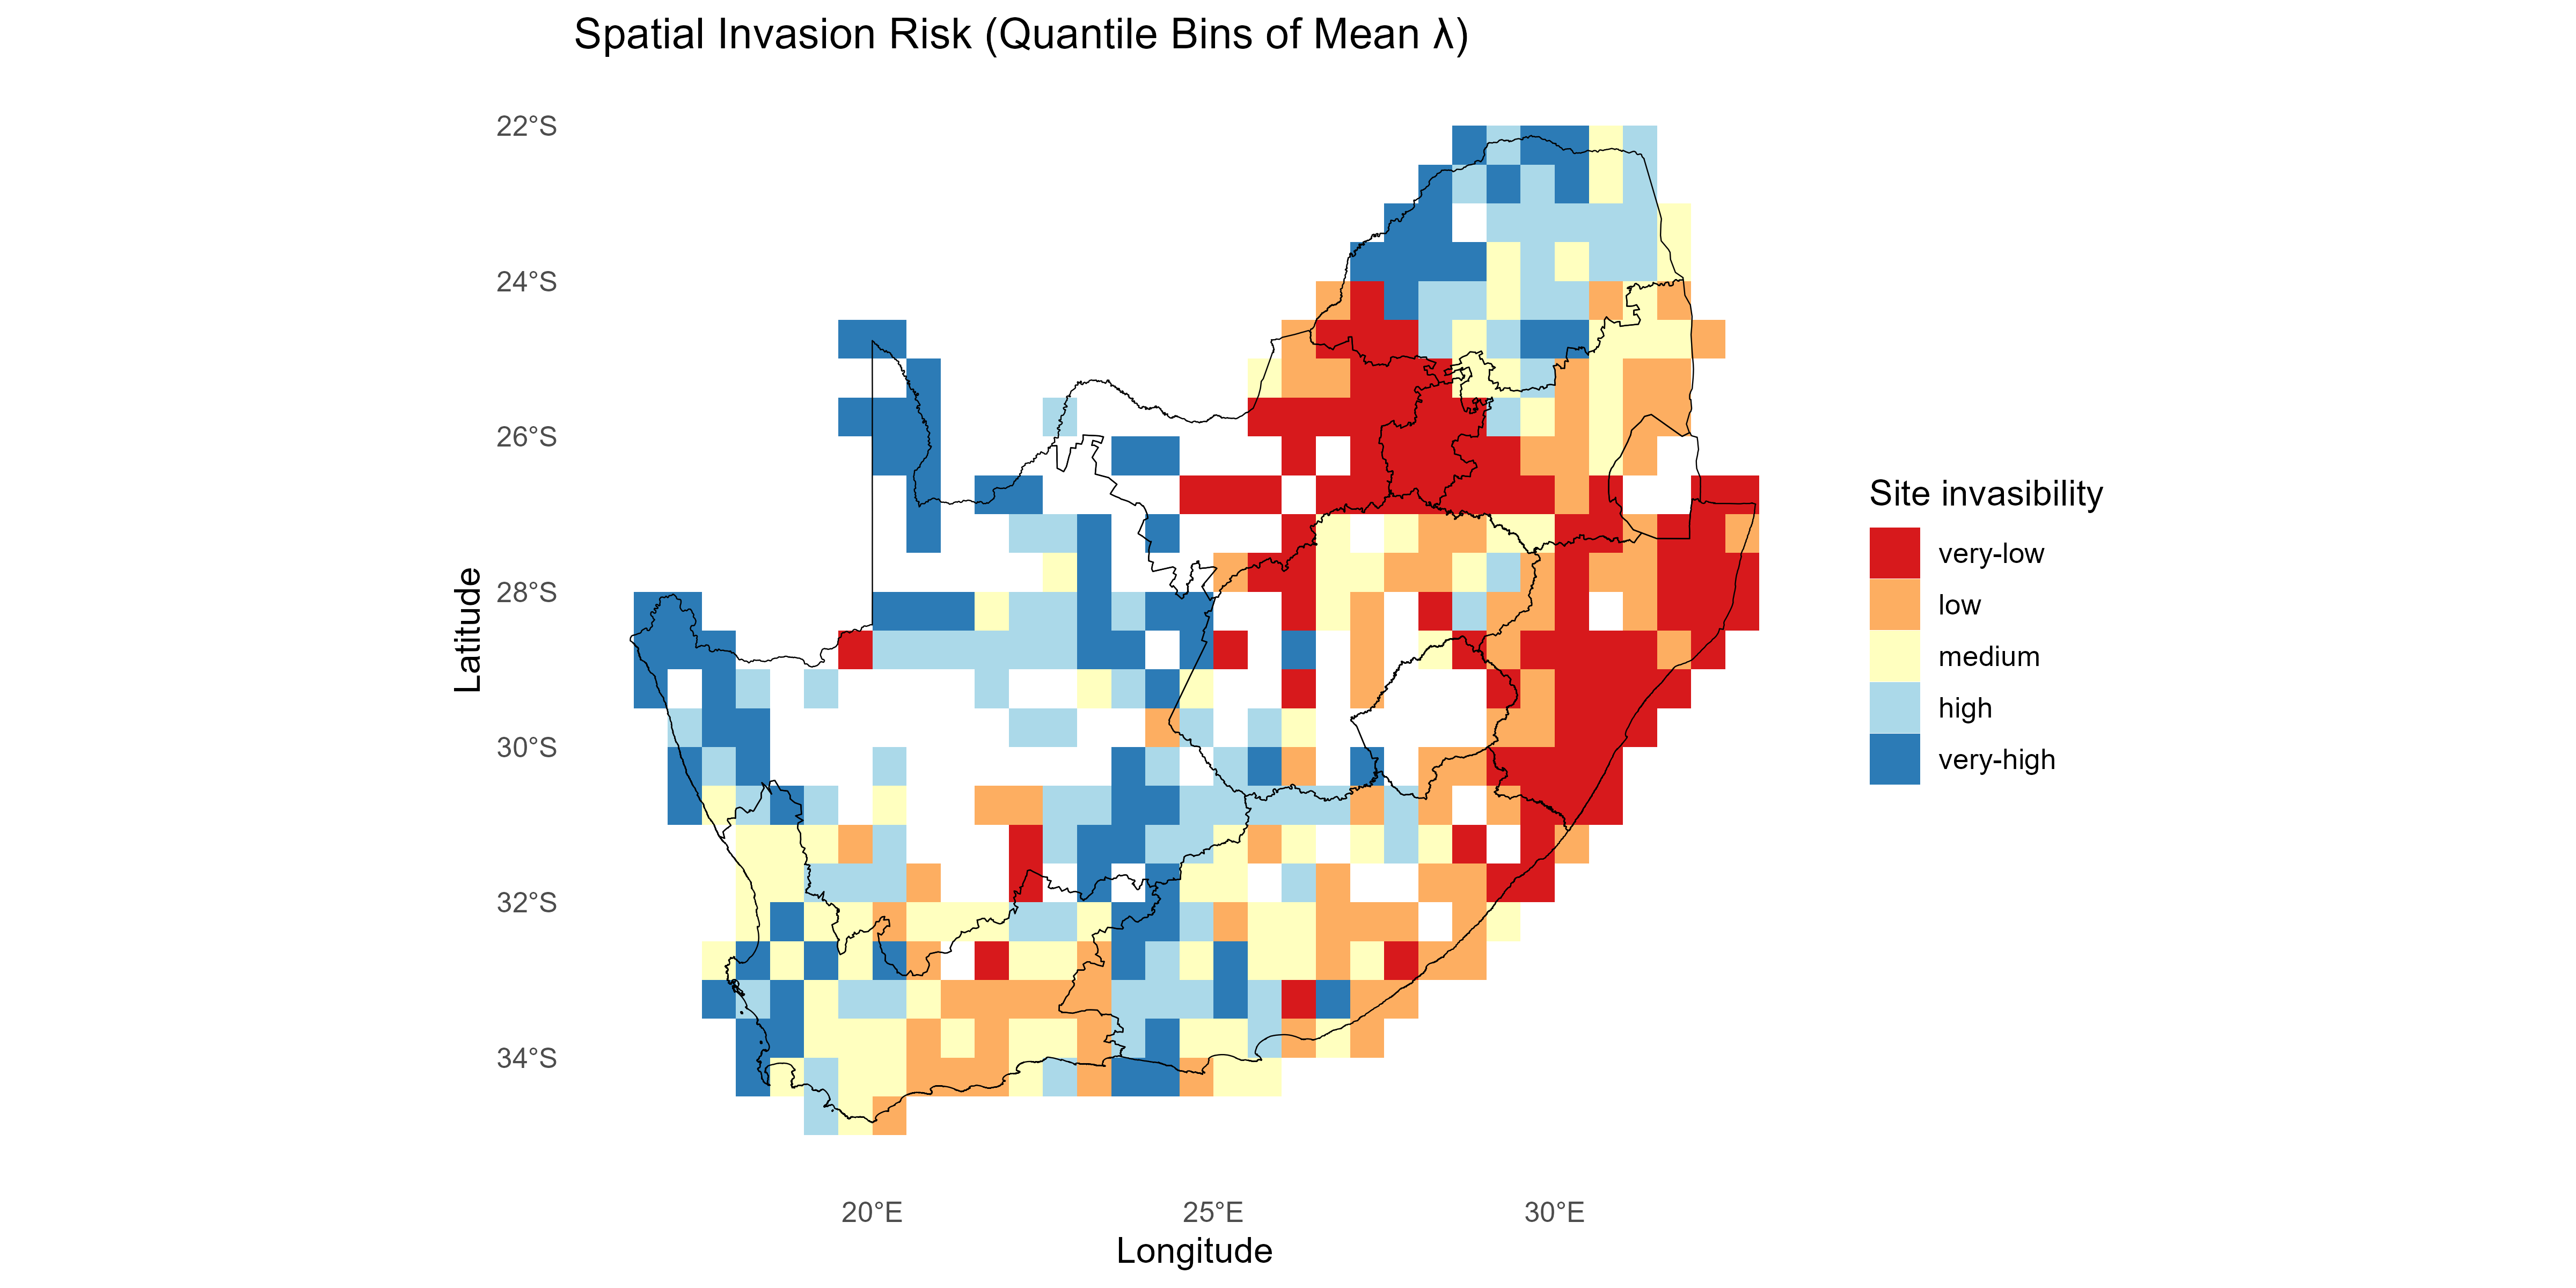
\includegraphics[width=1\linewidth]{man/figures/README-map-risk-1}

\hypertarget{analytical-summaries}{%
\subsection{11. Analytical Summaries}\label{analytical-summaries}}

These concise summaries complement spatial and cluster analyses,
providing direct insight into the most and least vulnerable sites, and
the most and least successful invaders, according to the modeled
invasion fitness landscape.

\hypertarget{distribution-of-invasion-fitness-values}{%
\subsubsection{11.1. Distribution of invasion fitness
values}\label{distribution-of-invasion-fitness-values}}

This histogram shows the overall distribution of invasion fitness
(\(\lambda_{i,k}\)) values for all invader-site pairs, indicating the
general ``openness'' of the community matrix and identifying the
prevalence of high-risk outcomes.

\begin{Shaded}
\begin{Highlighting}[]
\CommentTok{\# Plot the distribution of invasion fitness values (lambda) across all invader{-}site combinations,}
\CommentTok{\# using a histogram colored by lambda value for visual emphasis on fitness extremes}
\FunctionTok{ggplot}\NormalTok{(lambda\_df, }\FunctionTok{aes}\NormalTok{(}\AttributeTok{x =}\NormalTok{ lambda, }\AttributeTok{fill =}\NormalTok{ ..x..)) }\SpecialCharTok{+}
  \FunctionTok{geom\_histogram}\NormalTok{(}\AttributeTok{bins =} \DecValTok{40}\NormalTok{, }\AttributeTok{color =} \StringTok{"grey30"}\NormalTok{) }\SpecialCharTok{+}
  \FunctionTok{scale\_fill\_viridis\_c}\NormalTok{(}\AttributeTok{option =} \StringTok{"magma"}\NormalTok{, }\AttributeTok{guide =} \StringTok{"none"}\NormalTok{) }\SpecialCharTok{+}
  \FunctionTok{labs}\NormalTok{(}
    \AttributeTok{title =} \StringTok{"Distribution of Invasion Fitness Values (All Invader × Site)"}\NormalTok{,}
    \AttributeTok{x =} \FunctionTok{expression}\NormalTok{(}\StringTok{"Invasion Fitness"}\SpecialCharTok{\textasciitilde{}}\NormalTok{lambda[i}\SpecialCharTok{*}\NormalTok{k]),}
    \AttributeTok{y =} \StringTok{"Frequency"}
\NormalTok{  ) }\SpecialCharTok{+}
  \FunctionTok{theme\_minimal}\NormalTok{(}\AttributeTok{base\_size =} \DecValTok{12}\NormalTok{)}
\end{Highlighting}
\end{Shaded}

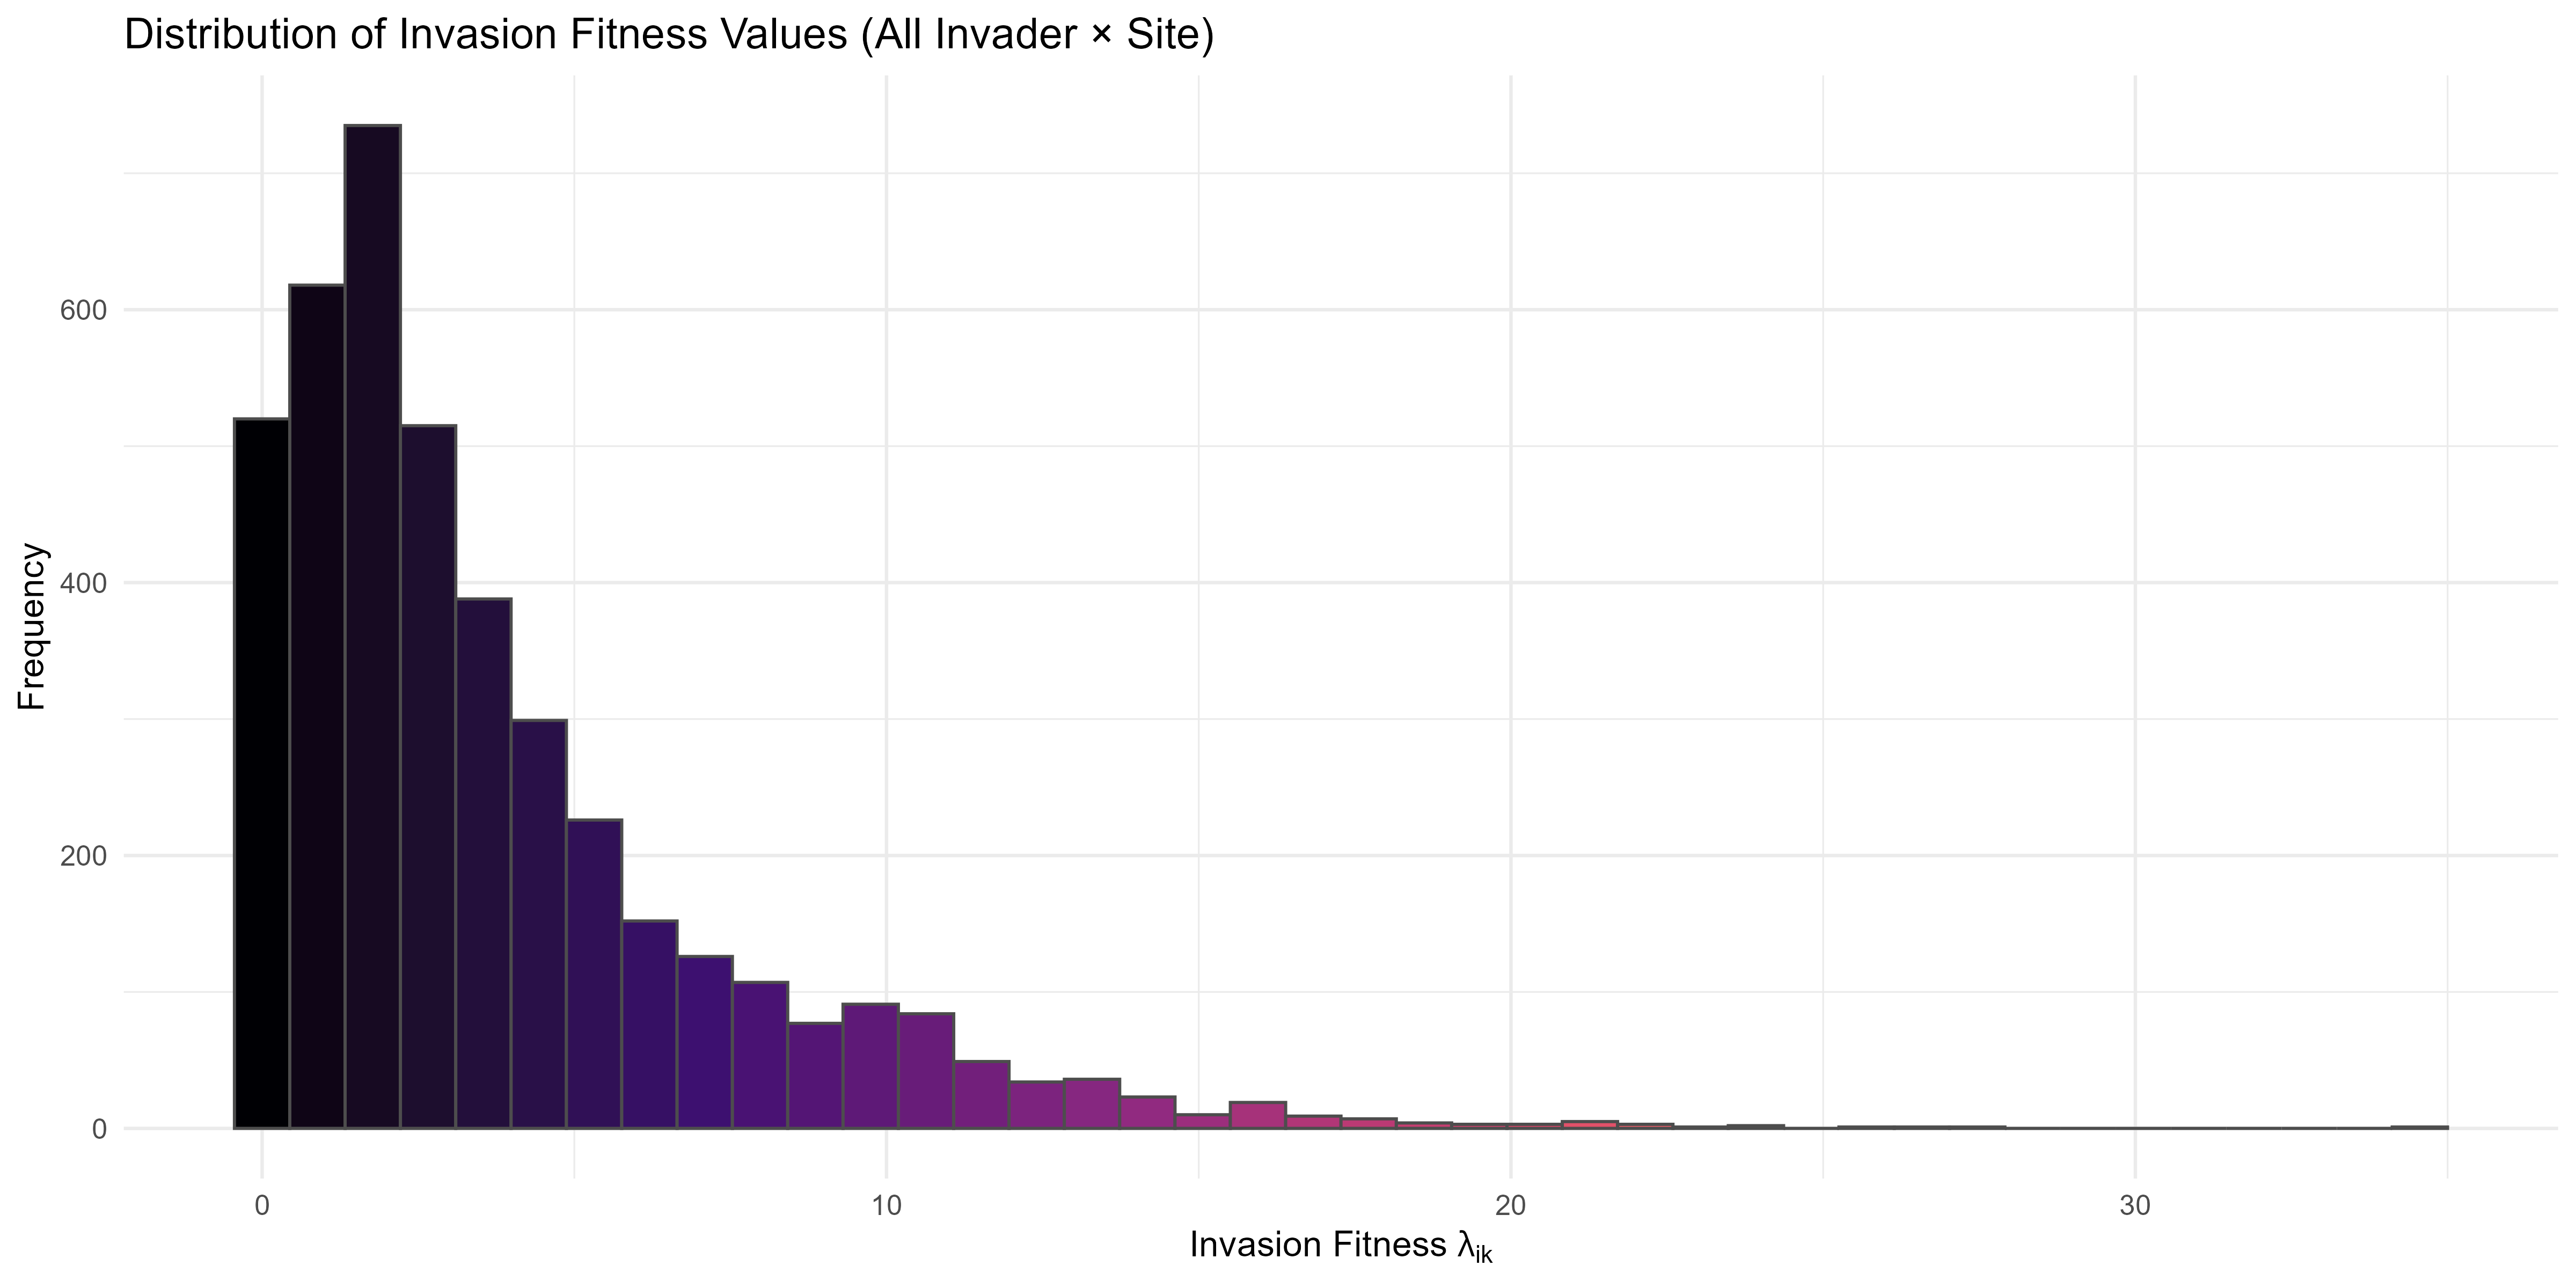
\includegraphics[width=1\linewidth]{man/figures/README-fitness-dist-1}

\hypertarget{topbottom-sites-and-invaders-by-mean-invasion-fitness}{%
\subsubsection{11.2. Top/bottom sites and invaders by mean invasion
fitness}\label{topbottom-sites-and-invaders-by-mean-invasion-fitness}}

This section reports the \textbf{top 3} and \textbf{bottom 3} invaders
and sites by mean invasion fitness, as plain-text console output. This
is useful for tabular reporting and rapid identification of outlier
risks.

\begin{verbatim}
#> ==== Top 3 Invaders by Mean Invasion Fitness ====
#> 1. inv5: 13.67
#> 2. inv9: 10.481
#> 3. inv8: 6.857
#> ==== Bottom 3 Invaders by Mean Invasion Fitness ====
#> 1. inv7: 2.612
#> 2. inv6: 2.383
#> 3. inv10: 2.134
#> ==== Top 3 Sites by Mean Invasion Fitness ====
#> 1. 494: 13.513
#> 2. 118: 13.44
#> 3. 122: 12.831
#> ==== Bottom 3 Sites by Mean Invasion Fitness ====
#> 1. 700: 2.607
#> 2. 663: 2.566
#> 3. 588: 2.507
\end{verbatim}

\hypertarget{trait-rankings-by-mean-invasion-fitness}{%
\subsubsection{11.3. Trait Rankings by Mean Invasion
Fitness}\label{trait-rankings-by-mean-invasion-fitness}}

To identify trait syndromes associated with invasion success or failure,
we aggregated invasion fitness scores (λ) by trait and calculated the
mean for each. The three traits with the highest mean λ values are
interpreted as those most strongly linked to successful invasion (i.e.,
``invasive'' traits), while the three with the lowest means are linked
to reduced invasion performance. This ranking provides an ecologically
interpretable, trait-based metric for prioritizing further functional or
mechanistic investigation.

\begin{verbatim}
#> ==== Top 3 Continuous Traits by Correlation with Mean Invasion Fitness ====
#> 1. trait_cont4: 0.377
#> 2. trait_cont10: 0.364
#> 3. trait_cont8: 0.353
#> 
#> ==== Bottom 3 Continuous Traits by Correlation with Mean Invasion Fitness ====
#> 1. trait_cont5: -0.442
#> 2. trait_cont2: -0.463
#> 3. trait_cont1: -0.627
#> ==== Categorical Traits: Top Value per Trait by Mean Invasion Fitness ====
#> trait_cat11: grassland (10.17)
#> trait_cat12: diurnal (7.10)
#> trait_cat13: bivoltine (8.45)
#> trait_cat14: nectarivore (8.98)
#> trait_cat15: resident (6.32)
\end{verbatim}

\hypertarget{faceted-site-maps-for-key-invaders}{%
\subsubsection{11.4. Faceted site maps for key
invaders}\label{faceted-site-maps-for-key-invaders}}

Finally, this faceted map visualizes \textbf{spatial patterns of
invasion fitness} for the top 3 and bottom 3 invaders, enabling
side-by-side comparison of their establishment potential across the
study region. This helps identify both ``super-invader'' strategies and
site-specific vulnerabilities or strengths.

\begin{Shaded}
\begin{Highlighting}[]
\CommentTok{\# Identify the top 3 and bottom 3 invaders by mean fitness}
\NormalTok{key\_invaders }\OtherTok{=} \FunctionTok{c}\NormalTok{(top3\_inv}\SpecialCharTok{$}\NormalTok{invader, bottom3\_inv}\SpecialCharTok{$}\NormalTok{invader) }\CommentTok{\# select 3 best/worst}

\CommentTok{\# Filter df amd ensure facet order matches ranking (top first, then bottom)}
\NormalTok{lambda\_key }\OtherTok{=}\NormalTok{ lambda\_df }\SpecialCharTok{\%\textgreater{}\%}
  \FunctionTok{filter}\NormalTok{(invader }\SpecialCharTok{\%in\%}\NormalTok{ key\_invaders) }\SpecialCharTok{\%\textgreater{}\%}
  \FunctionTok{mutate}\NormalTok{(}\AttributeTok{invader =} \FunctionTok{factor}\NormalTok{(invader, }\AttributeTok{levels =}\NormalTok{ key\_invaders)) }\CommentTok{\# enforce desired order}

\CommentTok{\# Faceted map}
\CommentTok{\# Spatial invasion fitness for each of the top/bottom invaders, enabling direct visual comparison}
\FunctionTok{ggplot}\NormalTok{(lambda\_key, }\FunctionTok{aes}\NormalTok{(}\AttributeTok{x =}\NormalTok{ x, }\AttributeTok{y =}\NormalTok{ y, }\AttributeTok{fill =}\NormalTok{ lambda)) }\SpecialCharTok{+}
  \FunctionTok{geom\_tile}\NormalTok{() }\SpecialCharTok{+}
  \FunctionTok{geom\_sf}\NormalTok{(}\AttributeTok{data =}\NormalTok{ rsa, }\AttributeTok{inherit.aes =} \ConstantTok{FALSE}\NormalTok{, }\AttributeTok{fill =} \ConstantTok{NA}\NormalTok{, }\AttributeTok{color =} \StringTok{"black"}\NormalTok{, }\AttributeTok{size =} \FloatTok{0.5}\NormalTok{) }\SpecialCharTok{+}
  \FunctionTok{facet\_wrap}\NormalTok{(}\SpecialCharTok{\textasciitilde{}}\NormalTok{invader, }\AttributeTok{ncol =} \DecValTok{3}\NormalTok{) }\SpecialCharTok{+}
  \FunctionTok{scale\_fill\_viridis\_c}\NormalTok{(}\AttributeTok{option =} \StringTok{"viridis"}\NormalTok{, }\AttributeTok{direction =} \SpecialCharTok{{-}}\DecValTok{1}\NormalTok{) }\SpecialCharTok{+}
  \FunctionTok{labs}\NormalTok{(}
    \AttributeTok{title =} \StringTok{"Spatial Summaries of Invasion Fitness}\SpecialCharTok{\textbackslash{}n}\StringTok{for Top{-}3 and Bottom{-}3 Invaders"}\NormalTok{,}
    \AttributeTok{x =} \StringTok{"Longitude"}\NormalTok{, }\AttributeTok{y =} \StringTok{"Latitude"}
\NormalTok{  ) }\SpecialCharTok{+}
  \FunctionTok{theme\_minimal}\NormalTok{(}\AttributeTok{base\_size =} \DecValTok{12}\NormalTok{) }\SpecialCharTok{+}
  \FunctionTok{theme}\NormalTok{(}\AttributeTok{panel.grid =} \FunctionTok{element\_blank}\NormalTok{())}
\end{Highlighting}
\end{Shaded}

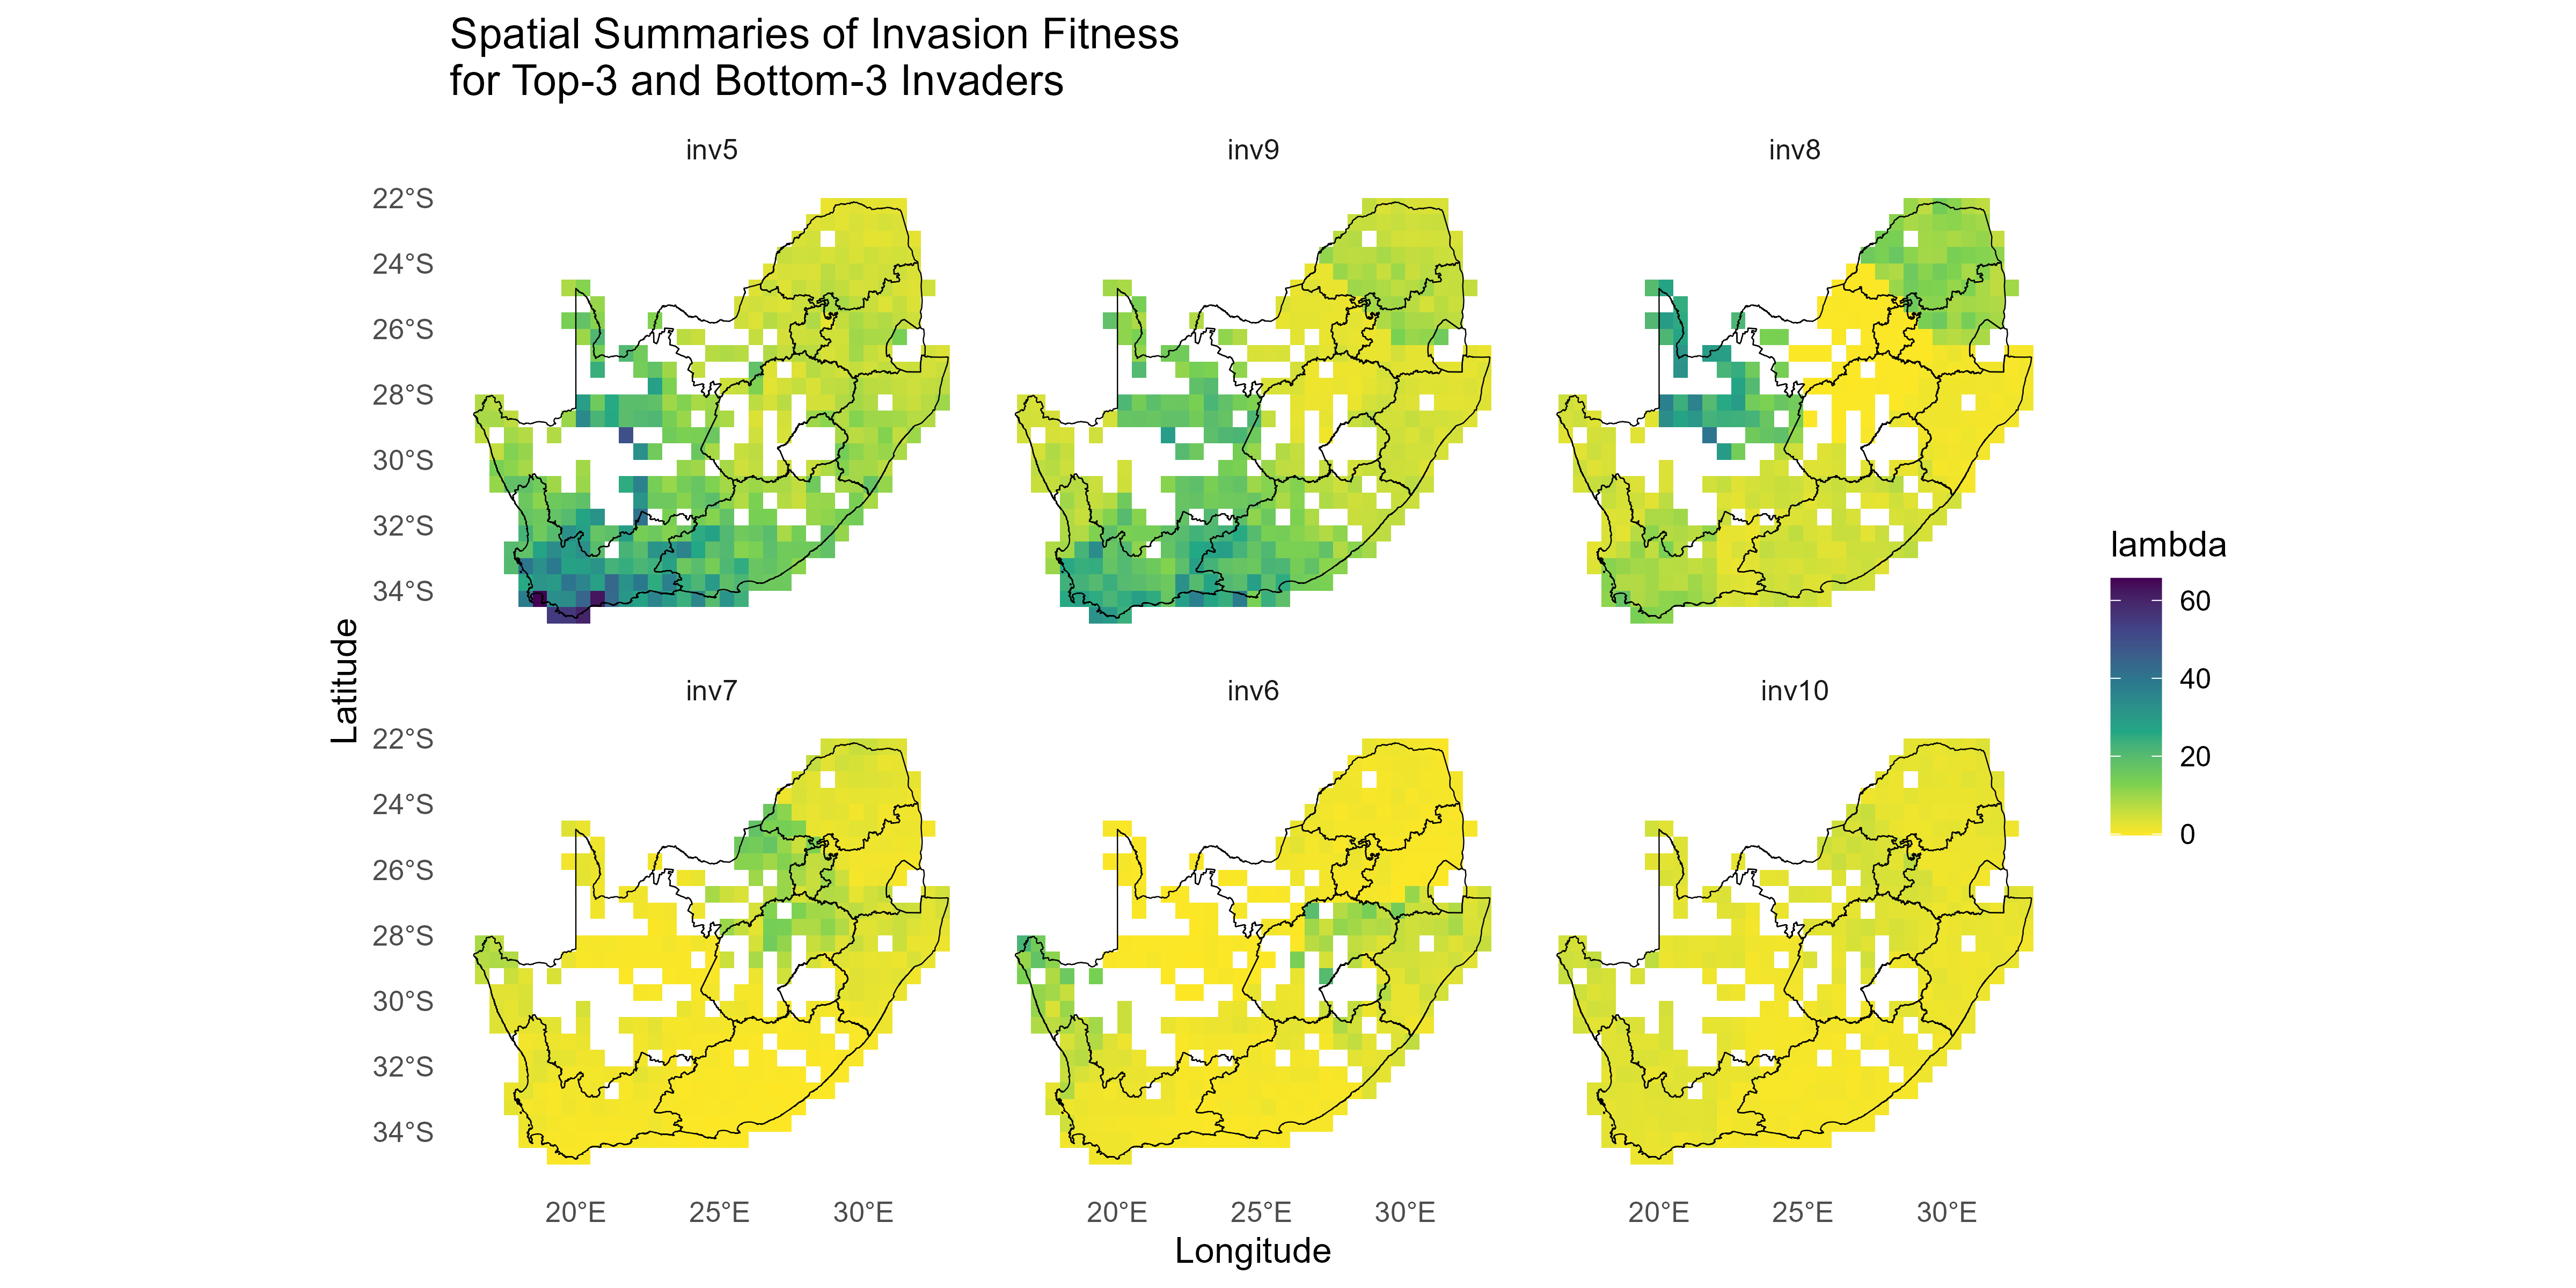
\includegraphics[width=1\linewidth]{man/figures/README-key-invaders-1}

\begin{quote}
\textbf{Summary:}

\begin{itemize}
\tightlist
\item
  \textbf{Clustered heatmaps} and \textbf{facet maps} reveal structure
  in invader/site response and vulnerability.
\item
  \textbf{Analytical summaries} allow targeting of monitoring or
  management to high-risk invaders/sites.
\item
  \textbf{Clustering} identifies ecological ``syndromes'' (groups of
  invaders/sites with similar invasion dynamics).
\end{itemize}
\end{quote}

\begin{center}\rule{0.5\linewidth}{0.5pt}\end{center}

\hypertarget{references}{%
\section{References}\label{references}}

\begin{itemize}
\tightlist
\item
  Hui C, Richardson DM (2017). Invasion Dynamics. Oxford University
  Press.
\item
  Hui C, Richardson DM, Landi P. et al.~(2016). Defining invasiveness
  and invasibility in ecological networks. Biological Invasions.
\item
  Hui C et al.~(2021). Trait-mediated ecological networks: mechanisms
  and consequences of invasion. Trends in Ecology \& Evolution.
\item
  \emph{Hui C et al.~(2023). {[}Title of relevant work, update as
  needed.{]}}
\end{itemize}

This RMarkdown document implements a reproducible, extensible workflow
for trait-based invasion ecology, integrating best practices for data
wrangling, statistical modeling, and scientific visualization. Please
cite the original data and framework sources as appropriate.

\end{document}
